% Copyright (C) 2014-2020 by Thomas Auzinger <thomas@auzinger.name>

\documentclass[draft,final]{vutinfth} % Remove option 'final' to obtain debug information.

% Load packages to allow in- and output of non-ASCII characters.
\usepackage{lmodern}        % Use an extension of the original Computer Modern font to minimize the use of bitmapped letters.
\usepackage[T1]{fontenc}    % Determines font encoding of the output. Font packages have to be included before this line.
\usepackage[utf8]{inputenc} % Determines encoding of the input. All input files have to use UTF8 encoding.
\newcommand{\nn}[1]{{\color{red}[#1]}}
% Extended LaTeX functionality is enables by including packages with \usepackage{...}.
\usepackage{amsmath}    % Extended typesetting of mathematical expression.
\usepackage{amssymb}    % Provides a multitude of mathematical symbols.
\usepackage{mathtools}  % Further extensions of mathematical typesetting.
\usepackage{microtype}  % Small-scale typographic enhancements.
\usepackage[inline]{enumitem} % User control over the layout of lists (itemize, enumerate, description).
\usepackage{multirow}   % Allows table elements to span several rows.
\usepackage{booktabs}   % Improves the typesettings of tables.
\usepackage{subcaption} % Allows the use of subfigures and enables their referencing.
\usepackage[ruled,linesnumbered,algochapter]{algorithm2e} % Enables the writing of pseudo code.
\usepackage[usenames,dvipsnames,table]{xcolor} % Allows the definition and use of colors. This package has to be included before tikz.
\usepackage{nag}       % Issues warnings when best practices in writing LaTeX documents are violated.
\usepackage{todonotes} % Provides tooltip-like todo notes.
\usepackage{hyperref}  % Enables cross linking in the electronic document version. This package has to be included second to last.
\usepackage[acronym,toc]{glossaries} % Enables the generation of glossaries and lists fo acronyms. This package has to be included last.

% Define convenience functions to use the author name and the thesis title in the PDF document properties.
\newcommand{\authorname}{M\'arcia R. Ferreira Gonçalves} % The author name without titles.
\newcommand{\thesistitle}{Pathways to Knowledge} % The title of the thesis. The English version should be used, if it exists.
%\setsubtitle{Essays on Academic Mobility and Institutional Prestige through Large-Scale Bibliographic and Digital Traces}

% Set PDF document properties
\hypersetup{
    pdfpagelayout   = TwoPageRight,           % How the document is shown in PDF viewers (optional).
    linkbordercolor = {Melon},                % The color of the borders of boxes around crosslinks (optional).
    pdfauthor       = {\authorname},          % The author's name in the document properties (optional).
    pdftitle        = {\thesistitle},         % The document's title in the document properties (optional).
    pdfsubject      = {Subject},              % The document's subject in the document properties (optional).
    pdfkeywords     = {a, list, of, keywords} % The document's keywords in the document properties (optional).
    }

\setpnumwidth{2.5em}        % Avoid overfull hboxes in the table of contents (see memoir manual).
\setsecnumdepth{subsection} % Enumerate subsections.

\nonzeroparskip             % Create space between paragraphs (optional).
\setlength{\parindent}{0pt} % Remove paragraph identation (optional).

\makeindex      % Use an optional index.
\makeglossaries % Use an optional glossary.
%\glstocfalse   % Remove the glossaries from the table of contents.

% Set persons with 4 arguments:
%  {title before name}{name}{title after name}{gender}
%  where both titles are optional (i.e. can be given as empty brackets {}).
\setauthor{}{\authorname}{BSc. MSc.}{female}
\setadvisor{Prof.}{Allan Hanbury}{}{male}

% For bachelor and master theses:
\setfirstassistant{Pretitle}{Forename Surname}{Posttitle}{male}
\setsecondassistant{Pretitle}{Forename Surname}{Posttitle}{male}
\setthirdassistant{Pretitle}{Forename Surname}{Posttitle}{male}

% For dissertations:
\setfirstreviewer{Pretitle}{Forename Surname}{Posttitle}{male}
\setsecondreviewer{Pretitle}{Forename Surname}{Posttitle}{male}

% For dissertations at the PhD School and optionally for dissertations:
\setsecondadvisor{Prof.}{Stefan Thurner}{}{male}{} % Comment to remove.

% Required data.
\setregnumber{11929255}
\setdate{31}{05}{2023} % Set date with 3 arguments: {day}{month}{year}.
\settitle{\thesistitle}{{Pathways to Knowledge}} % Sets English and German version of the title (both can be English or German). If your title contains commas, enclose it with additional curvy brackets (i.e., {{your title}}) or define it as a macro as done with \thesistitle.
\setsubtitle{Essays on academic mobility through large scale bibliographic and digital traces} % Sets English and German version of the subtitle (both can be English or German).
% Select the thesis type: bachelor / master / doctor / phd-school.
% Bachelor:
%\setthesis{bachelor}
%
% Master:
%\setthesis{master}
%\setmasterdegree{dipl.} % dipl. / rer.nat. / rer.soc.oec. / master
%
% Doctor:

\setthesis{doctor}
\setdoctordegree{rer.soc.oec.}% rer.nat. / techn. / rer.soc.oec.
%
% Doctor at the PhD School
\setthesis{phd-school} % Deactivate non-English title pages (see below)

% For bachelor and master:
%\setcurriculum{Media Informatics and Visual Computing}{Medieninformatik und Visual Computing} % Sets the English and German name of the curriculum.

% For dissertations at the PhD School:
\setfirstreviewerdata{Prof. Roberta Sinatra, University of Copenhagen, Denmark}
\setsecondreviewerdata{Prof. Mirta Galesic, Santa Fe Institute, United States}


\begin{document}

\frontmatter % Switches to roman numbering.
% The structure of the thesis has to conform to the guidelines at
%  https://informatics.tuwien.ac.at/study-services

%\addtitlepage{naustrian} % German title page (not for dissertations at the PhD School).
\addtitlepage{english} % English title page.
\addstatementpage

%\begin{danksagung*}
%\todo{Ihr Text hier.}
%\end{danksagung*}

\begin{acknowledgements*}
I want to give warm thanks to my supervisors, Stefan Thurner (Principal) and Vito Servedio. Their  academic supervision and the breadth of their knowledge have always been an example to me. Stefan's relentless pursuit of excellence has pushed me to expand my thinking and analysis, shaping a more resilient scientist in me. Vito, with his unique perspective, and clear and insightful suggestions, has enriched my understanding of the field of network science and broadened my research horizons. Both supervisors taught me a new way of thinking and approaching research. I am indebted to my co-supervisor Allan Hanbury, who not only guided me through the milestones of my PhD journey but also introduced me to the fascinating world of Informatics at TU Wien. All three supervisors gave me the opportunity to deepen my research skills in different teams and projects and were caring, wise and friendly.

A heartfelt thank you goes to my mentor and friend Rodrigo Costas. Rodrigo's invaluable guidance at every stage of this PhD has been instrumental in shaping both my interests and the trajectory of my work. I have cherished our past projects together and look forward to many more in the future. I also thank Ludo Waltman for numerous discussions from the start of my journey in Science of Science and help with kickstarting the development of the Talent Flows Webtool developed in this project. Ludo was a kind mentor who was always willing to share valuable connections with me. 

My gratitude extends to Ed Noyons, whose unshakeable kindness and uncompromising honesty have marked him as an exceptional supervisor and director. Ed treated me as a valued colleague long after I left the excellence halls of the Centre for Science and Technology Studies (CWTS) at Leiden University. I am also thankful to Mark Neijssel, Clara Medina Calero, Carole Pottier, Henri de Winter, Bijan Ranjbar-Saharei, and Nees van Eck, and many others at CWTS who have collectively shaped my way of thinking about research assessment and bibliometrics. They demonstrated that the vision of a more equitable research system is not an intangible dream nestled in the clouds of utopia, but rather, a tangible goal that can be shaped with collective hands. It is a testament to the CWTS tenacity, wisdom, and guidance that I am able to envisage this reality and be braver.

A special mention goes to Michele Pasin, Juergen Wastl, Johannes Sorger, Wolfgang Kneck, Liuhuaying Yang, and Tobias Batik, who generously invested their time in helping me create the Talent Flows Webtool and offered me key technical help and feedback. I also thank Frank Neffke, William Schueller, and Maria del Rio-Chanona, who not only gave me their time generously, but also followed up with further advice.

I fondly remember and appreciate the camaraderie of my colleagues and friends Niklas, Vito and Simone in the Innovation Dynamics Group. I look forward to many more stimulating discussions, foosball, italian meals and barbecues. Another thank you goes to all my CSH colleagues and friends, I have enjoyed our times together by the coffee machine and beyond.

A final word of thanks goes to my beloved partner and family. Their contributions to this work, are less direct, yet indispensable.
\end{acknowledgements*}


\begin{kurzfassung}
\todo{Ihr Text hier.}
\end{kurzfassung}

\begin{abstract}

It is difficult to put a value on scientific research. Since the 1980s, scientific assessments in universities and other research organizations based on quantitative metrics have become more central. The most common metric at the journal level is the controversial impact factor (IF). But there are also metrics for individuals. The h-index is an equally controversial measure: a scientist with an index of 5 has published 5 papers which have each been cited at least five times. These metrics presumably capture impact and productivity and have major implications for staffing and funding, research priorities, innovation programmes, and recognition. \textit{The problem?} Researchers and universities are often rewarded based on input and output metrics that may not represent ‘quality’ and may not clearly guide strategic decision-making. Significant disparities in the number of researchers, funding for research, economic development, infrastructure, endogenous capabilities and skills, make it more crucial to understand the observed differences in scientific performance and quality. New indicators are thus needed to address the opportunities and gaps in knowledge production and dissemination in different research contexts. The interconnectedness of scientific skills, the interaction and collaboration of scholars, technology, and the geography of institutions form an intricate web of knowledge advancement. Therefore, using metrics without understanding the long-term process of knowledge creation and interactive learning has led, and, still is, likely to lead to sub-optimal outcomes. 

In this doctoral thesis, we delve into the complex terrain of scientific progress and its dynamics, examining the various pathways to scientific knowledge creation and how this know-how is expressed in publication data. We focus on the interconnected aspects of innovation and knowledge flows in science such as \textit{exaptation}, \textit{academic inbreeding}, \textit{skill alignment}, \textit{academic mobility} at institutions and regions as well as the accumulation of regional knowledge capabilities, the dynamics of \textit{citation networks}, and finally the role of social media (i.e., \textit{altmetrics}) in scientists' workflow. 

In Chapter 1, we quantify, for the first time, the signatures of exaptation, where old ideas find new life in breakthrough applications in the context of science. We propose two indicators: a normalized entropy and inverse participation ratio indicator to reveal patterns of exaptation and its role in scientific innovation. By clustering the citation network of a set of publications in physics, we show that our measures allow us to filter out patterns related to exaptation phenomena in scientific evolution. In Chapter 2, we address the challenges of the rapidly changing citation network. We find that as scientific progress accelerates, the lifespan of scientific publications also decreases. We use a microscopic generative model to study the growth of publications and the power law phenomenon of forgetting, which raises questions about the sustainability of the current scientific system.

Chapter 3 takes us inside academic institutions, where we examine the growing global phenomenon of institutional mobility. Using data from the Dimensions database and the Global Research Identifier Database, we discover different trends in researcher mobility between institutions in Europe and North America. In this chapter, we also uncover patterns of skill alignment among researchers within institutions and offer a new understanding of how institutional prestige, internal collaboration, and geographic location affect the flow of knowledge and skills. In Chapter 4, we broaden the perspective of our research to examine the accumulation process of regional scientific capabilities and their impact on global technological leadership. Our main finding is that early investment in emerging research areas is an important driver of scientific dominance. This ``rich-get-richer'' phenomenon underlies the development of scientific strength in a region. In Chapters 3 and 4, we use data on scientific activities, topics, institutions, and geographic locations, as well as on researcher mobility, to identify strategies that regions and institutions can use to attract scientists and achieve scientific dominance in a given research area.

Finally, in Chapter 5, we venture into the realm of alternative metrics, or altmetrics, and examine the symbolic capital derived from researchers' Twitter activities and its relationship to traditional scholarly capital captured through citations. This analysis is facilitated by a novel method for identifying scientists with Twitter accounts.


\end{abstract}

% Select the language of the thesis, e.g., english or naustrian.
\selectlanguage{english}

% Add a table of contents (toc).
\tableofcontents % Starred version, i.e., \tableofcontents*, removes the self-entry.

% Switch to arabic numbering and start the enumeration of chapters in the table of content.
\mainmatter

% ======================== INTRODUCTION ===================================

\chapter{Introduction}

\section{Problem statement}

\section{Databases}

\section{Publications and contributions}

\section{Research questions}

\section{Structure of the thesis}

% ========================= CHAPTERS ======================================	
\chapter{Measuring science}

To understand the differences in research performance and impact, it is not enough to count the number of citations a scholar, university, region or country has received in the past. We therefore propose that research metrics are examined in relation to other dimensions such as capacity to learn, existing skills, capabilities, and networks that may provide alternative evaluative solutions and facilitate interactive learning and innovation. 
% ========================= CHAPTERS ======================================	
\chapter{Exaptation: Re-purposing scientific knowledge}

The rediscovery of a new function for a given object or concept can be just as important as its discovery. This phenomenon is known as \emph{exaptation}, and the related verb is \emph{to co-opt}. It characterises the process of acquiring new functions for which a trait, which originally evolved to solve one problem, is co-opted to solve a new problem \cite{gould1982exaptation}. The definition is similar to the concept of \emph{preadaptation}~\cite{bock1959preadaptation}. However, since this term may suggest teleology, Vrba and Gould urged scholars to replace that term by exaptation. The idea of exaptation was also proposed to distinguish the concept from \emph{adaptation}~\cite{darwin2004origin}. While exaptations are traits that have applications that deviate from their original purpose~\cite{gould1982exaptation,kauffman2000investigations}, adaptations have been shaped by natural selection for their current use~\cite{bock1959preadaptation,darwin2004origin}. One canonical example of exaptation in biology is the evolution of feathers.  It is often argued that feathers were not originally developed for flight, but emerged in the reptilian ancestors of today's birds for thermal regulation~\cite{gould1982exaptation}.  Other examples include the ability of a metabolic reaction network to survive on different food sources which can allow adoption of alternative substrates \cite{barve2013latent}.
Exaptation events seem to be important to give birth to adaptive innovations, diversity and, more generally, to complex traits~\cite{barve2013latent}.

Gould and Vrba propose exaptations have adaptive and non-adaptive origins: \emph{preaptation} and \emph{nonaptation}. Preaptation refers to characteristics or traits that are adapted and `selected' for one evolutionary purpose (adaptations). These are later co-opted to serve another purpose leading to an increase in the fitness of the co-opted trait. Thus, preaptations are adaptations that have undergone a significant change in function~\cite{gould1982exaptation,lloyd2017exaptation}. Another source of exaptation is nonaptation. Nonaptation refers to traits that emerge through a process of trial and error that generates lots of `leftover' features (e.g., DNA, molecules, cells)~\cite{gould1982exaptation}. These concern the effective use of co-opted leftover traits to serve a particular function, but whose origin cannot be ascribed to the process of `natural selection' \cite{gould1982exaptation}. Nonaptations are byproducts of the evolution of some other trait ~\cite{darwin2004origin} that do not add to the fitness of the co-opted trait \cite{lloyd2017exaptation,gould1982exaptation}. In summary, adaptations, preaptations, and nonaptations are essential processes that drive the evolution of living matter, cells, humans, organisms, and biological ecosystems.  They allow us to understand the adaptive and non-adaptive origins of biological novelty.

\section{Exaptation in science and technology}
Recently, the notion of exaptation has been applied to the study of technological change \cite{bonifati2010more,dew2004economic}. One set of studies have focused on the development of technological speciation narratives~\cite{dew2004economic,levinthal1998slow,andriani2013exaptation} and niche construction theory~\cite{dew2016exaptation}. Other studies focused on the adoption of technology~\cite{rogers2010diffusion}, its commercial application~\cite{schumpeter1939business}, and its economic impact~\cite{dew2016exaptation}, but not on the origin of those inventions \cite{fleming2004science}. Small-scale studies of technological exaptation abound in the management and innovation literature (e.g., \cite{tan2015alexander, dew2016exaptation, cattani2005preadaptation,rosenman1988serendipity}). These studies point to the role of chance such as serendipitous discovery of a new function \cite{andriani2013exaptation}. Serendipity (accidental circumstances leading to fortunate findings)  and exaptation (a shift in the function of something) are intricately related by the fact that accidental discoveries that contribute to the redeployment of a component in a different context lead to a shift in the function of that component.

A related stream of research has attempted to model the dynamics of invention mathematically by analysing specific knowledge spaces~\cite{tria2014dynamics,loreto2016dynamics,thurner2010schumpeterian,klimek2010evolutionary,klimek2012empirical,hidalgo2009building,tacchella2012new,servedio2018new,kauffman1993origins, gabora2013quantum}. The aim of these studies is not to explain why some entities produce more innovations than others (productivity), or what influences the ability of these entities to produce them, but how knowledge evolves in a mechanistic view. 
These studies have provided evidence for the existence of innovation bursts in national economies~\cite{thurner2010schumpeterian,klimek2012empirical}, the rediscovery of publications leading to the emergence of new scientific fields~\cite{thurner2019role,van2004sleeping}, and the novel combination of components as a source of everyday novelties~\cite{tria2014dynamics}. 
Few attempts focused on explicitly quantifying exaptation, one notable exception being~\cite{andriani2017measuring}, where it is estimated that about 40\% of pharmaceutical drugs have started as something else. 

Similarly, many scientific discoveries find applications that are not foreseen from the outset. The scientific context is particularly relevant for the study of exaptation since it encompasses a variety of human activities where knowledge is frequently rediscovered and re-used.
In scientific evolution processes, different disciplines may come together, ``to tell one coherent interlocking story``~\cite{watson2017convergence}, or a field may subdivide into new disciplines. Both may form the basis on which concepts can further recombine. The recent use of statistical physics to examine people's behaviour in crowds, traffic, or stock markets is an example of co-opting theories and techniques to the social sciences. Research on laser technologies~\cite{bonifati2010more}, pharmaceuticals~\cite{andriani2017measuring}, and fibre optics~\cite{cattani2005preadaptation} keep expanding their scope of application in very diverse fields. This kind of re-purposing may enhance (though not necessarily) the fitness of entities~\cite{gould1982exaptation}. Exaptation in the context of science thus refers to a diversification logic, where publications build on an existing knowledge base and succeed in entering other fields by creating new scientific niches or sub-fields. We thus interpret exaptation in science as how research insights from publications in one field are co-opted (i.e., cited) by publications from different scientific domains.

A growing number of scholars in the area of innovation theory propose exaptation as the ultimate source of novelty. They argue that exaptation can explain the emergence of markets, technologies, and technical functions~\cite{dew2016exaptation,cattani2005preadaptation,andriani2017measuring,mokyr1991evolutionary}. In their view, exaptation leads to \emph{technological speciation} or the creation of \emph{technological niches}~\cite{andriani2016exaptation}. In technological speciation processes, new technology develops from the effective transfer of existing knowledge to a new situation, where the transferred knowledge is interpreted and exploited in new ways~\cite{cohen1990absorptive}. Famous cases that illustrate this pattern include Corning Inc., a company that used its long-standing experience on glass engineering to deliver ground-breaking fibre-optic work that has transformed the telecommunications landscape~\cite{watson2017convergence}, or the microwave, which was discovered by chance through the repurposing of parts of a radar system~\cite{rosenman1988serendipity}. Often, a distinction is made between radical and incremental innovations. While radical innovations transform the technological landscape, incremental innovations are minor improvements in existing technologies~\cite{dewar1986adoption}. Exaptation has been associated with radical innovations leading to the creation of new technological niches~\cite{andriani2013exaptation}. Most empirical studies of exaptation in those contexts have been limited to small-scale or narratives of specific technologies.

In the context of science, contributions to the study of invention have used scientific publications, and metadata, such as author affiliation, organisation, location, and citation linkages to assess novel research outputs. Citation network analysis has been used extensively. Uzzi et al.~\cite{uzzi2013atypical} used co-citation linkages from publications in various fields to differentiate between typical and atypical co-citations. Atypical co-citations are papers that are rarely cited together. They found that high-impact publications were usually not those that had the most atypical or novel combination of ideas, nor those that used typical combinations of ideas, but papers that cite a mix of new and conventional ideas. This result implies that, while originality is a crucial feature of high-impact science, the building blocks for new ideas are often embodied in existing knowledge~\cite{uzzi2013atypical}. Further, papers with high novelty as measured by atypical combinations tend to be less cited at the start, but are more likely to be cited after several years after publication~\cite{stephan2017reviewers}. Other studies, which highlight the role of recombining ideas in driving innovation, suggest that older, seminal works are more likely to inspire ground-breaking science~\cite{kuhn1962structure}. 

The combination of different theories, fields, and tools is also central to interdisciplinary research~\cite{wagner2011approaches}. Interdisciplinarity is likely to lead to more `innovative' research~\cite{thurner2019role}, which is associated with higher levels of citation impact~\cite{lariviere2015long}. Furthermore, the citation influence of papers is enhanced by the thematic distance (i.e., cognitively different fields) from the articles they cite \cite{klavans2013towards}. Yet, such outputs often face more resistance than mainstream publications (i.e., publications drawing mainly on the knowledge of a single field), thus requiring more time to get recognised by the wider scientific community \cite{thurner2019role}. This idea relates to the ``first-mover`` advantage where mediocre papers will often receive more citations early on, than a later excellent one \cite{newman2009first}. There is, however, conflicting evidence that interdisciplinary research obtains higher citation rates at the level of journals in natural and medical sciences \cite{levitt2008multidisciplinary}, research departments \cite{rinia2002impact}, and in the field of biomedicine \cite{lariviere2010relationship}. 
This evidence shows that the relationship between novel research - as defined by interdisciplinary combinations - and impact depends on the characteristics of the fields and type of analysis involved \cite{lariviere2010relationship}.

\section{Quantifying exaptation in science}
To track scientific progress, we use the APS dataset~\cite{apsdataset}, which includes publications in the leading physics journals since 1893. Following~\cite{blondel2008fast}, we apply the Louvain algorithm to design an alternative classification scheme that clusters the set of all publications (articles and reviews) in the APS between 1893 and 2017 into research areas. The method is based on first determining pairs of publications that cite one another, and second, on clustering publications into a research area. The procedure uses a directed citation network where nodes consist of publications and links consist of citations between publications. Each publication belongs to a unique research area. We disregard the direction of the links in the network and exclude publications without citations.

%
\begin{figure}[b]
    \centering
    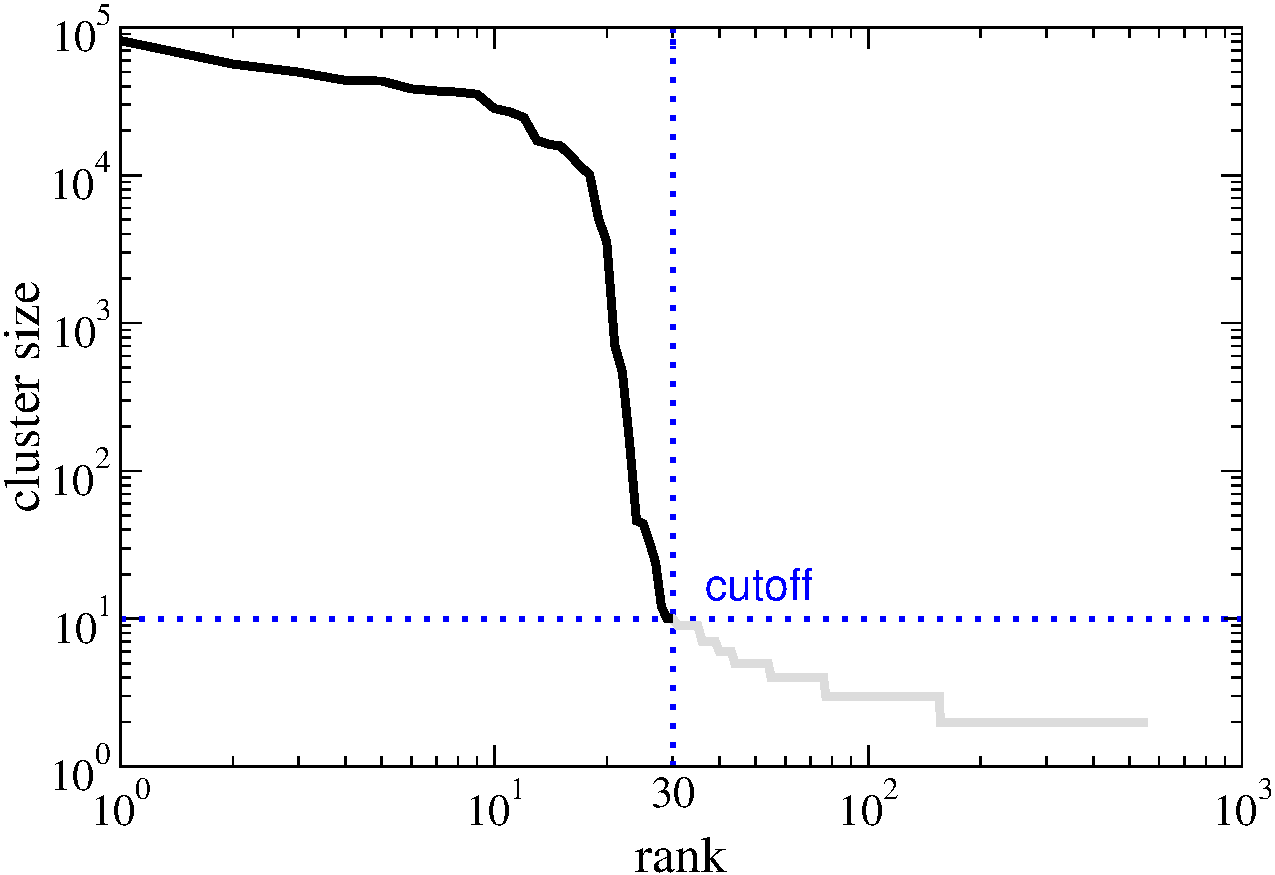
\includegraphics[width=0.55\textwidth]{figures_exaptation/clustersize.pdf}
    \caption{Cluster size vs rank.
    The number of APS articles in a cluster as a function of  the rank of the clusters.
    Clusters were detected by the Louvain algorithm applied to the citation network. 
    We cluster all articles appeared in APS from 1893 to 2017. 
    In our analysis, we remove the articles belonging to clusters with less than 10 articles. 
    These removed clusters constitute a few percent of all articles.}
    \label{fig:cluster_sizes}
\end{figure}
%
Fig.~\ref{fig:cluster_sizes} shows the distribution of cluster sizes. For several clusters the number of publications is very small. For practical reasons we excluded clusters that have less than 10 publications. This method allows us to examine the influence of publications that belong to a specific field on other papers pertaining to different fields. This information is essential to determine whether a paper has been co-opted by papers in another field. This also allows us to trace the bibliographic properties of the citing publications.
%
\begin{figure}[t]
  \centering
  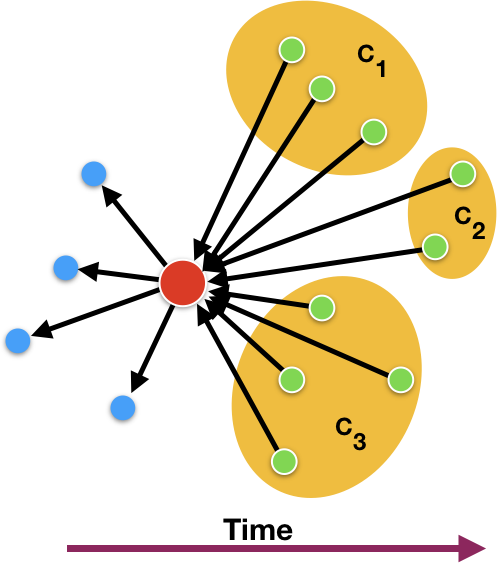
\includegraphics[width=0.45\textwidth]{figures_exaptation/fwd-entropy.png}
  \caption{Definition of normalised forward entropy cartoon.
    Circles represent published articles and arrows stand for citations. 
    Only those articles and links are displayed, which are relevant for the entropy definition. The article $a_i$ denoted with the large red circle cites four papers (blue circles at its left side) and has been cited by nine papers (green circles on its right side). These nine articles belong to three different clusters $C_n$ depicted as orange ovals. Denoting with $p_n$ the fraction of articles of cluster $n$ in the whole citation pool of the red article, we have $p_1=1/3$, $p_2=2/9$ and $p_3=4/9$. According to Eq.~(\ref{eq:fwd_entropy}), the normalised forward entropy is then $S_i=(-1/3 \log 1/3 - 2/9 \log 2/9 - 4/9 \log 4/9)/\log 3 \approx 0.966$. The IPR for $a_i$ is $I_i \simeq 2.79$.}
  \label{fig:fwd_entropy}
\end{figure}
%
To quantify the idea of functionality, we define a quantity that we call {\em forward normalised entropy} (FNE), $S_i$, of a generic article  $a_i$. In Fig.~\ref{fig:fwd_entropy}, we consider the articles citing  $a_i$ (red circle), each belonging to a cluster, $C_n$, here we use all papers published in APS until 2017. Denoting by $A_i$ the set of articles citing $a_i$ and by $C_n$ the clusters in the system, we define $p_{i,n} = |C_n\cap A_i| / |A_i|$. In other words, $p_{i,n}$ is the fraction of articles citing the reference article $a_i$, that belong to cluster $C_n$. We define the normalised forward entropy, $S_i$,  as:
%
\begin{equation}
  S_i = -\frac{1}{\log N_i}\sum_{n=1}^{N_i} p_{i,n} \log p_{i,n}\ ,
  \label{eq:fwd_entropy}
\end{equation}
%
\noindent where $N_i$ is the number of clusters for which $p_{i,n}>0$.
We call $S_i$ a forward entropy because it is computed based on articles published after $a_i$ and citing $a_i$.

It gives information on how heterogeneous the composition of the citing articles is in terms of cluster composition. If an article is cited by articles belonging to only one cluster, i.e., it belongs to a well-defined scientific field, $S_i=0$. If a paper has $S_i=1$, then its citations are uniformly distributed among different areas. Therefore, the forward entropy can be thought of as a score for interdisciplinary impact.

To estimate the effective number of clusters from which the paper $a_i$ received citations, we consider the Inverse Participation Ratio (IPR) $I_i$ of article $a_i$: 
\begin{equation}
    I_i = \left(\sum_{n, p_{i,n}>0} (p_{i,n})^{-2}\right)^{-1}.
    \label{eq:ipr}
\end{equation}
Its value approximates the number of effective clusters citing $a_i$. We calculate the forward entropy and IPR for every year, by considering only those articles published in a given year, and citing $a_i$. In this way, we can follow the trajectory of an article over time, keeping track of the scientific areas it belonged to.

\section{Results}
\subsection{The signatures of exaptation}

We considered all publications in the APS database until 2017 and selected the top 200 most cited ones. 
The reasons for using highly cited publications are both conceptual and pragmatic. 
First, we assume that exaptation results from the significant adoption or acknowledgement of a paper. 
This implies that a co-opted publication should have a high citation impact. 
Second, a large number of citations enhances the statistical significance of the results. 
To identify distinctive patterns of exaptation, we looked at the yearly number of citations vs.\ the forward normalised entropy (FNE), $S_i$, and the IPR, $I_i$, for all articles. We present a few examples with a well-defined signature of exaptation. 

Before that, let us clarify how this pattern should ideally look like. 
A good candidate article for exaptation, say $a_\mathrm{ex}$, ideally belongs to a well-established field and is disciplinary in nature. 
If the paper initially received citations only by papers in the same scientific sub-field, then its FNE score, $S_i$, would be zero. 
We hypothesise that at some point in time, the number of citations to $a_\mathrm{ex}$ starts increasing and possibly remains in the same scientific sub-field. 
At a later stage, the article may start receiving citations by papers from other scientific sub-fields, causing $S_i$ to increase. 
The very fact that papers are co-opted in another scientific sub-domain also brings more citations to $a_\mathrm{ex}$. 
%
If the new citing domain is highly productive, i.e., with many published papers, then $S_i$ may eventually decline, as most of the citations will now come from the new citing field, overshadowing the original one. 
Eventually, while the citation rate of the paper will start to decrease as a natural consequence of ageing, its FNE, on the contrary, may increase slightly as other fields may become interested in the article and grow in relative importance.

%
\begin{figure}[t]
    \centering
    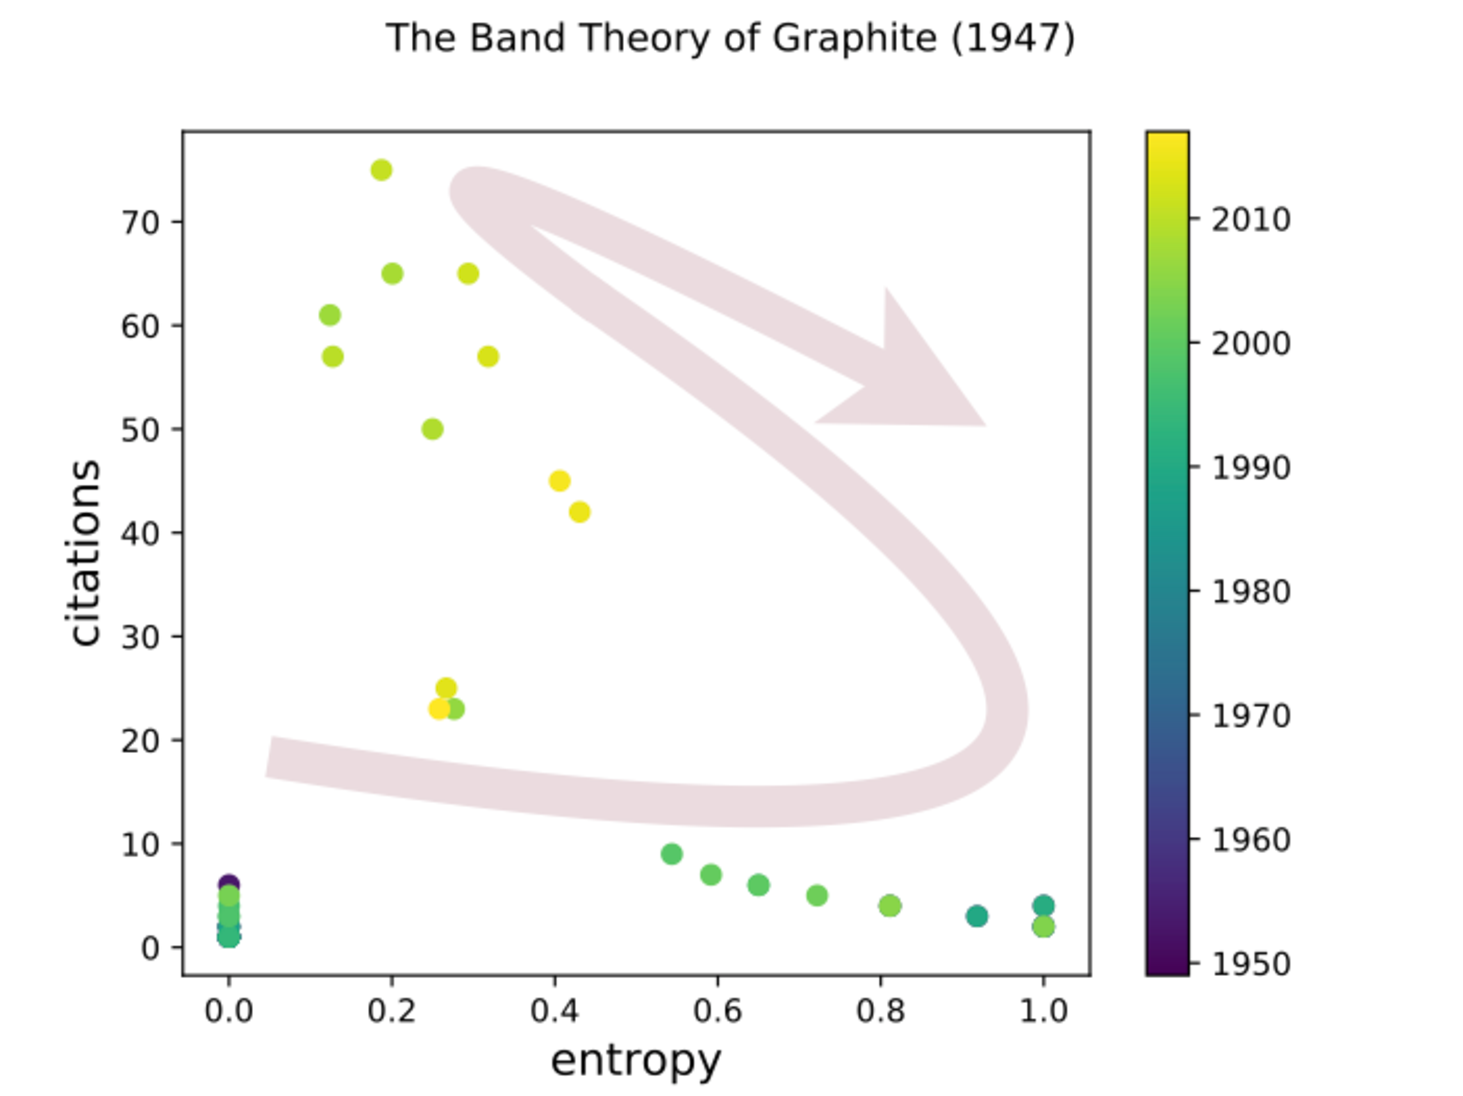
\includegraphics[width=0.45\textwidth]{figures_exaptation/graphene-entropy.pdf}%
    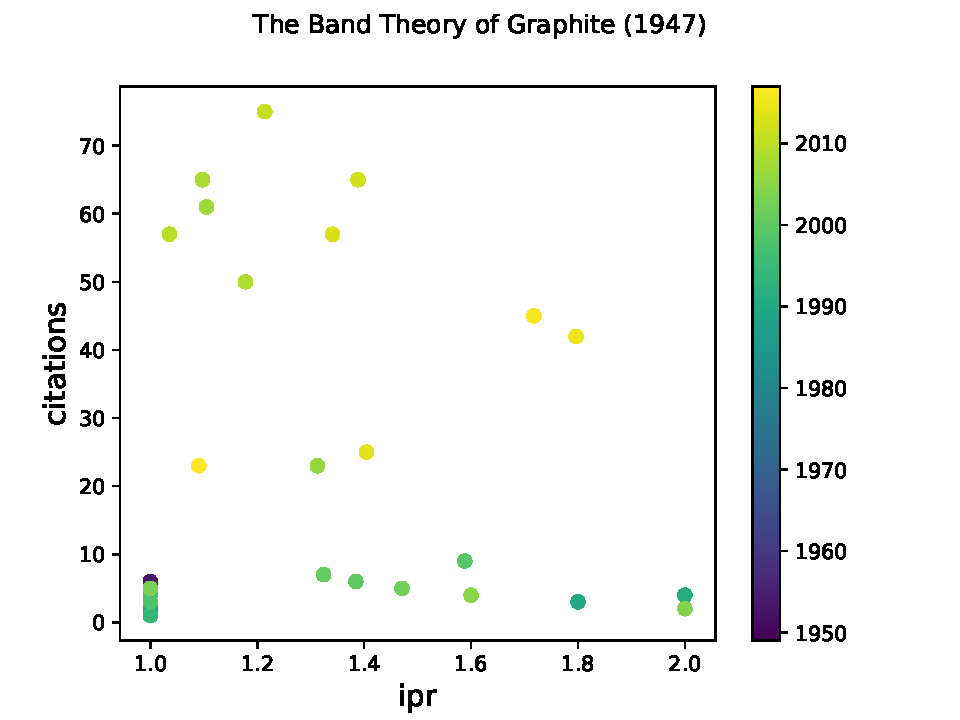
\includegraphics[width=0.45\textwidth]{figures_exaptation/graphene-ipr.pdf}
    \caption{A typical pattern for exaptation of an important paper.
    {Left:} yearly number of citations vs.\ the forward normalised entropy of the paper of Ref.\cite{graphite1947}. Each circle represents a different year, and the time-evolution is marked with a colour code, from dark tones (older) to light ones (newer). The ideal dynamics of citations and entropy over time for an exapted paper is also depicted by a thick arrow.
    The paper starts in one field ($S_i=0$), then is exapted in another field leading to an increase of $S_i$; then, citations grow since the paper gets more popular while $S_i$ decreases, since the new field prevails; eventually, the number of citations decreases as an ageing effect while $S_i$ increases again, since the paper is rediscovered in the older field.
    {Right:} yearly number of citations vs.\ IPR of~\cite{graphite1947}.}
    \label{fig:graphene}
\end{figure}
%
The paper \emph{The band theory of graphite}, published in 1947~\cite{graphite1947} seems to follow the hypothesised pattern of exaptation. 
Before taking a closer look, let us first dig into the graphene background.
%
Graphite is a material made up of carbon atoms arranged in parallel hexagonal layers. 
Like the diamond, it is an allotropic form of carbon. 
While graphite is a conductor at room temperature, the diamond is an insulator. 
To understand why the carbon atoms with different crystal geometries are conducting or insulating it is necessary to understand how electrons behave once an electrical potential is applied.
One of the great success of quantum mechanics was the possibility to understand these phenomena.
The electronic structure of simple materials became computable right after the formalism of quantum mechanics was established. 
The geometry of graphite suggests that its electronic properties can be incrementally determined by first analysing a single layer of carbon - what is today known as \textit{graphene} - and then by considering the mutual interaction between layers. As Wallace wrote in his manuscript~\cite{graphite1947}:
\begin{quote}
 Since the spacing of the lattice planes of graphite is large (3.37\AA) compared with the hexagonal spacing in the layer (1.42\AA), a first approximation in the treatment of graphite may be obtained by neglecting the interactions between planes, and supposing that conduction takes place only in layers.
\end{quote}
%
\noindent 
Wallace did not consider the possibility  that a hexagonal layer of carbon atoms could exist by itself and used it as a mere tool to solve the ``more complicated'' problem for the three-dimensional graphite. 
As recently pointed out in a review essay on graphene~\cite{graphene_review2009}:
\begin{quote}
 It was P.~R.~Wallace, who in 1946 wrote the first papers on the band structure of graphene and showed the unusual semi-metallic behaviour in this material (Wallace, 1947). At that point in time, the thought of a purely 2D structure was a mere fantasy and Wallace's studies of graphene served him as a starting point to study graphite, a very important material for nuclear reactors in the post-World War II era.
\end{quote}
%

%
\begin{figure}[t]
    \centering
    \begin{tabular}{cc}
    Word cloud for the graphene cluster&
    Word cloud for the ESP cluster\\
    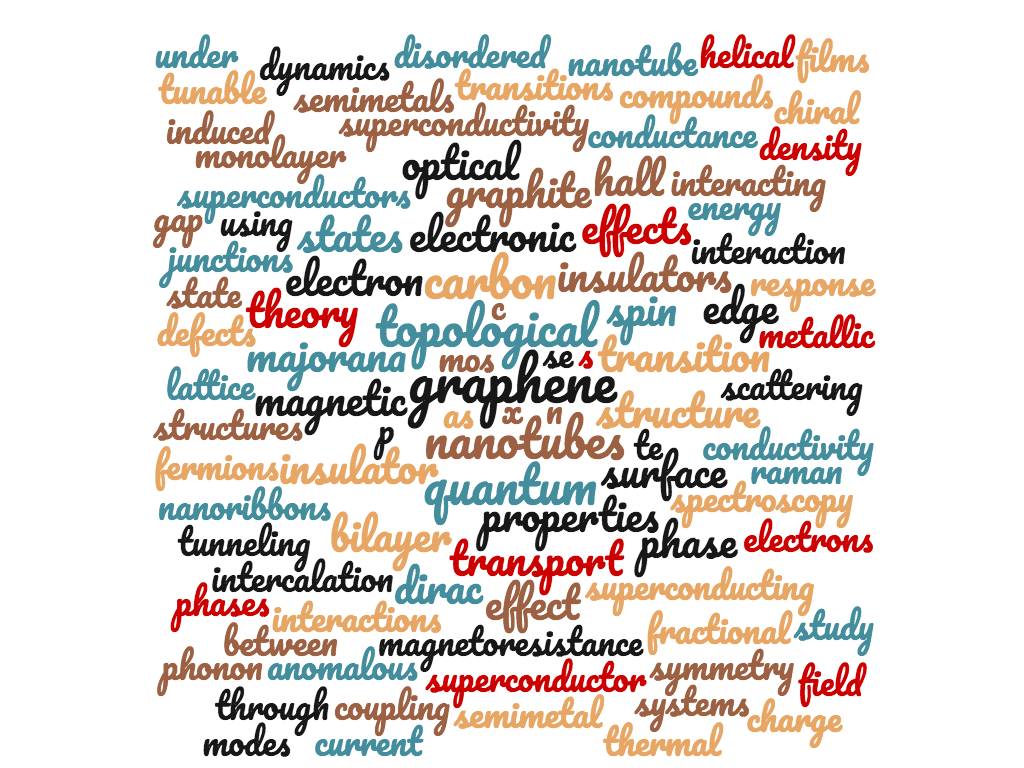
\includegraphics[width=0.40\textwidth]{figures_exaptation/wordcloud-graphene1.png}&
    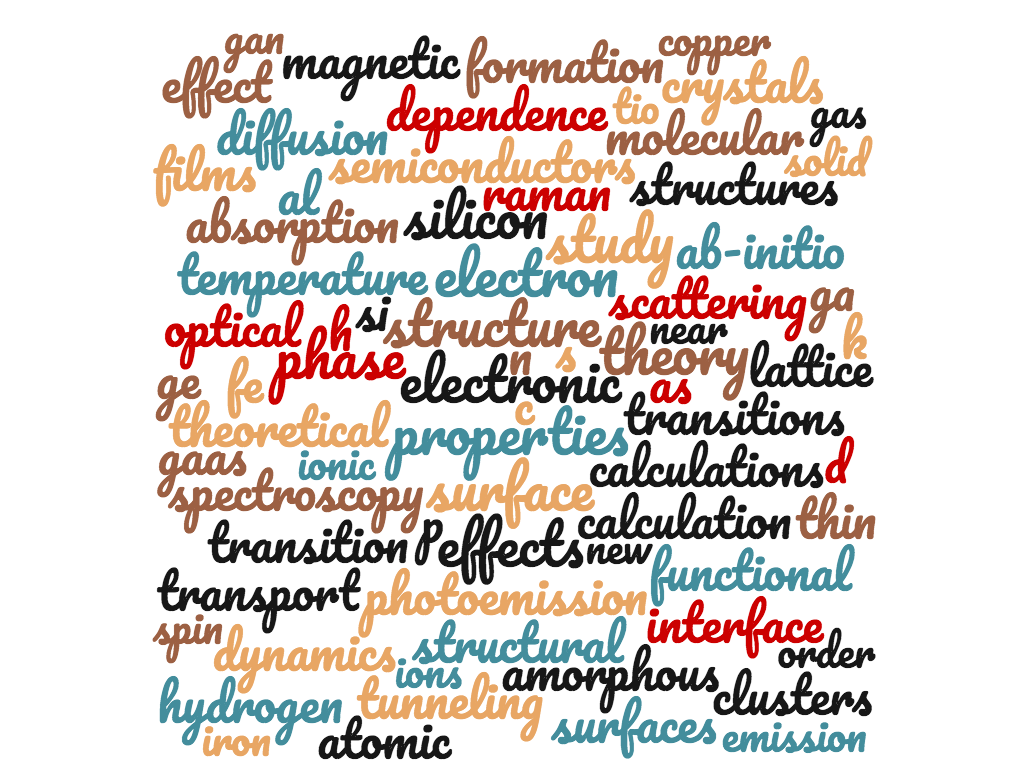
\includegraphics[width=0.40\textwidth]{figures_exaptation/wordcloud-graphene2.png}
    \end{tabular}
    \caption{Word clouds of the two communities citing Wallace's paper.
    Word clouds~\cite{wordcloud} were generated by merging all the titles belonging to the main two clusters citing the graphite/graphene article. Stop words, numbers and punctuation marks were removed. Font size is proportional to the logarithm of the number of occurrences of words. The composition of the main cluster (graphene) with 613 articles citing Wallace's graphite article \protect\cite{graphite1947} is shown on the left; the second important cluster (electronic structure properties) with 33 articles is on the right.
    }
    \label{fig:wordclouds}
\end{figure}
%
Let us see now why the seminal paper of Wallace on graphene can be considered an example of exaptation according to the pattern highlighted above. Figure~\ref{fig:graphene}, shows two panels of the yearly number of citations vs.\ the forward normalised entropy (FNE) $S_i$ (left), and the IPR, $I_i$ (right). 
The paper starts with a small number of citations and a very small FNE (bottom-left corner of the plot in the left panel). 
After that, the pattern follows a very peculiar ``S-shaped'' trajectory, mirroring the following three situations: (i) the adoption by another field leading to an increase of $S_i$, (ii) the growth in the number of citations while $S_i$ decreases, (iii) the decrease of the number of citations while $S_i$ increases again.

This suggests that Wallace's article that was meant to belong to the field of electronic structure properties (ESP), was later co-opted in the graphene research field. 
According to the cluster analysis, the ESP field contains approximately 12,000 articles and the much more recent graphene area contains about 5,000 articles. 
Despite the larger number of articles in ESP, Wallace's paper has been cited mostly by the graphene community (613 times), and much less from the  ESP (33 times). 
The forward normalised entropy of this paper follows the exaptation pattern we assumed. 
Its IPR pattern (Fig.~\ref{fig:graphene} (right panel)) demonstrates how it switched from the ESP to the graphene community. 
To visualise the differences between the two ESP and graphene communities, in Fig.~\ref{fig:wordclouds} we show two word-clouds from the articles citing Wallace's paper: from the graphene community  (left) and the ESP one (right). 

We found 10 additional articles whose FNE and IPR patterns are similar to those of the graphite/graphene paper. Among those, we mention two notable examples, i.e., \emph{Motion of Electrons and Holes in Perturbed Periodic Fields}~\cite{electrons_and_holes} and \emph{Quantized Hall Conductance in a Two-Dimensional Periodic Potential}~\cite{quantized_hall}. 
A third article, that was not in the list of the most 200 cited papers but was highly cited from outside the APS, was chosen on the basis of our personal experience, \emph{Spin Echoes}~\cite{spin_echoes}. 
The first ~\cite{electrons_and_holes}, is mainly cited by articles belonging to two clusters,  the ``Quantum dots / Quantum wells'' cluster (QDQW) and the ESP cluster. These clusters are denoted by id=8 and id=1 respectively, and their mutual importance is sketched in the plots on the right panels of Fig.~\ref{fig:examples}.  
Note how after 1980, the QDQW cluster starts to become more important than ESP, so that~\cite{electrons_and_holes} acquires more importance in that field. 
A similar situation occurs with reference ~\cite{quantized_hall} (second row of the panel), where now the graphene cluster (id=16) competes with the QDQW cluster. Interestingly, from year 2010 on, also the ``Bose-Einstein condensate'' cluster (id=12) starts to get some importance.

\begin{figure}[t]
    \centering
    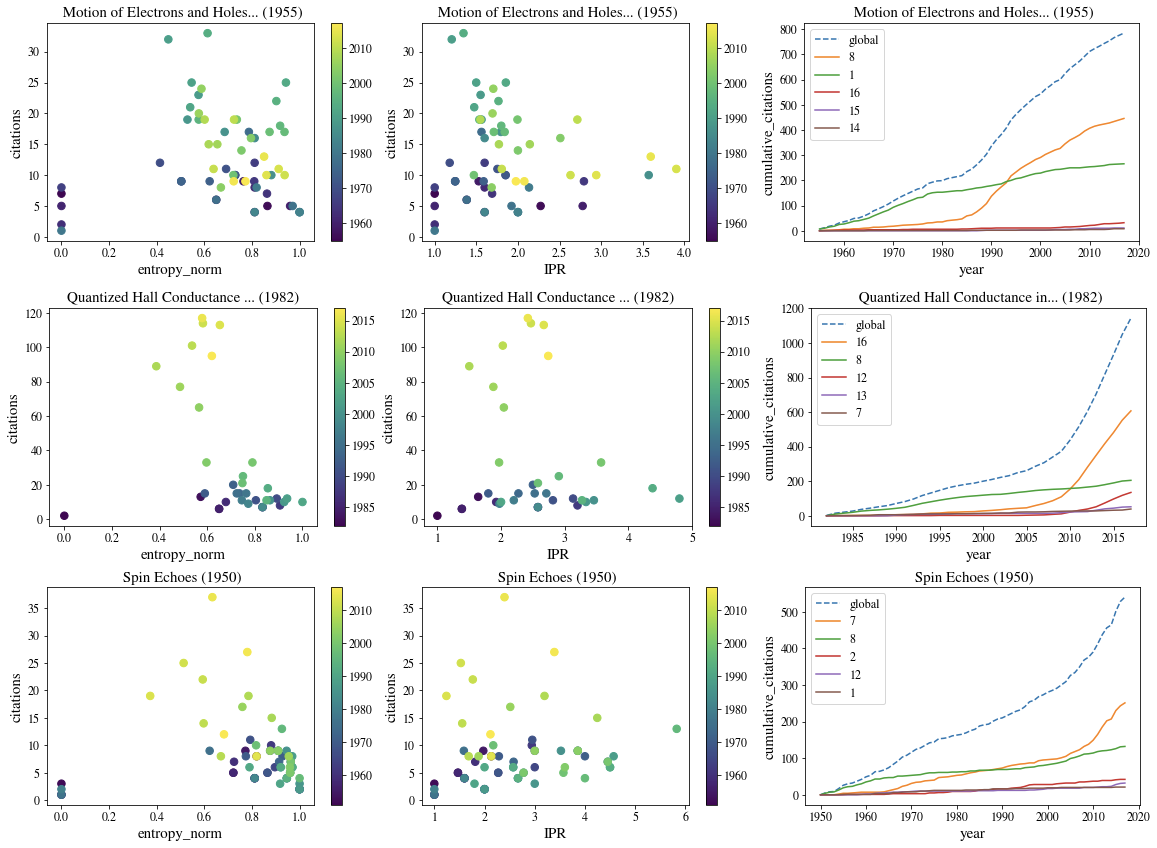
\includegraphics[width=0.95\textwidth]{figures_exaptation/exaptation_examples.png}
    \caption{More examples of exaptation patterns. Three articles are shown: Refs.~\protect\cite{electrons_and_holes,quantized_hall,spin_echoes}, one in each row. In the left and centre panels, we display their citation versus FNE and IPR, respectively. Patterns are similar to what was found in Fig.~\ref{fig:graphene}. In panels to the right, we show the time evolution of their cumulative citations in the respective clusters, whose id number is given in the legend. Their vertical order reflects their ranking in 2017, i.e., their relative importance in citing the selected paper.}
    \label{fig:examples}
\end{figure}

The third paper on spin echoes was chosen since we expected its importance on Nuclear Magnetic Resonance (NMR) would become prominent in time (third row of the panel). 
We do not observe a clear NMR cluster in APS, rather we find an exaptation pattern, where the ``Entanglement'' cluster (id=7) emerges on the detriment of the QDQW cluster (id=8), as shown in the bottom right panel. 
We think that the NMR community cites this paper from outside the APS community, i.e., by papers not published by the APS journals.
%

Although not directly related to the problem of detecting exaptation in APS articles, it is worthwhile looking at the time evolution of the FNE and the IPR for review articles. We observe the same kind of pattern consistently in all highly cited APS review papers. As an example, we show the Chandrasekhar's review \emph{Stochastic problems in physics and astronomy}~\cite{review1943}; the corresponding plots for FNE and IPR are reported in Fig.~\ref{fig:review}.
Both FNE and IPR increase over time, witnessing the number of different scientific fields interested in the review. The manuscript itself~\cite{review1943} features four chapters, the problem of random flights, the theory of the Brownian motion, probability after effects, and probability methods in stellar dynamics. The IPR  value reaches the value four soon and oscillates around it in time. On the other hand, the FNE, after reaching its maximum value, starts to decrease, mainly because one citing field increases its importance over the others. The IPR and FNE behaviour of highly cited reviews is essentially different from the patterns found for co-opted articles presented in Figs.~\ref{fig:examples} and \ref{fig:graphene}. This finding further reassures us of the robustness of the proposed indicators, as well as of the overall methodology. 
%
\begin{figure}[t]
  \centering
  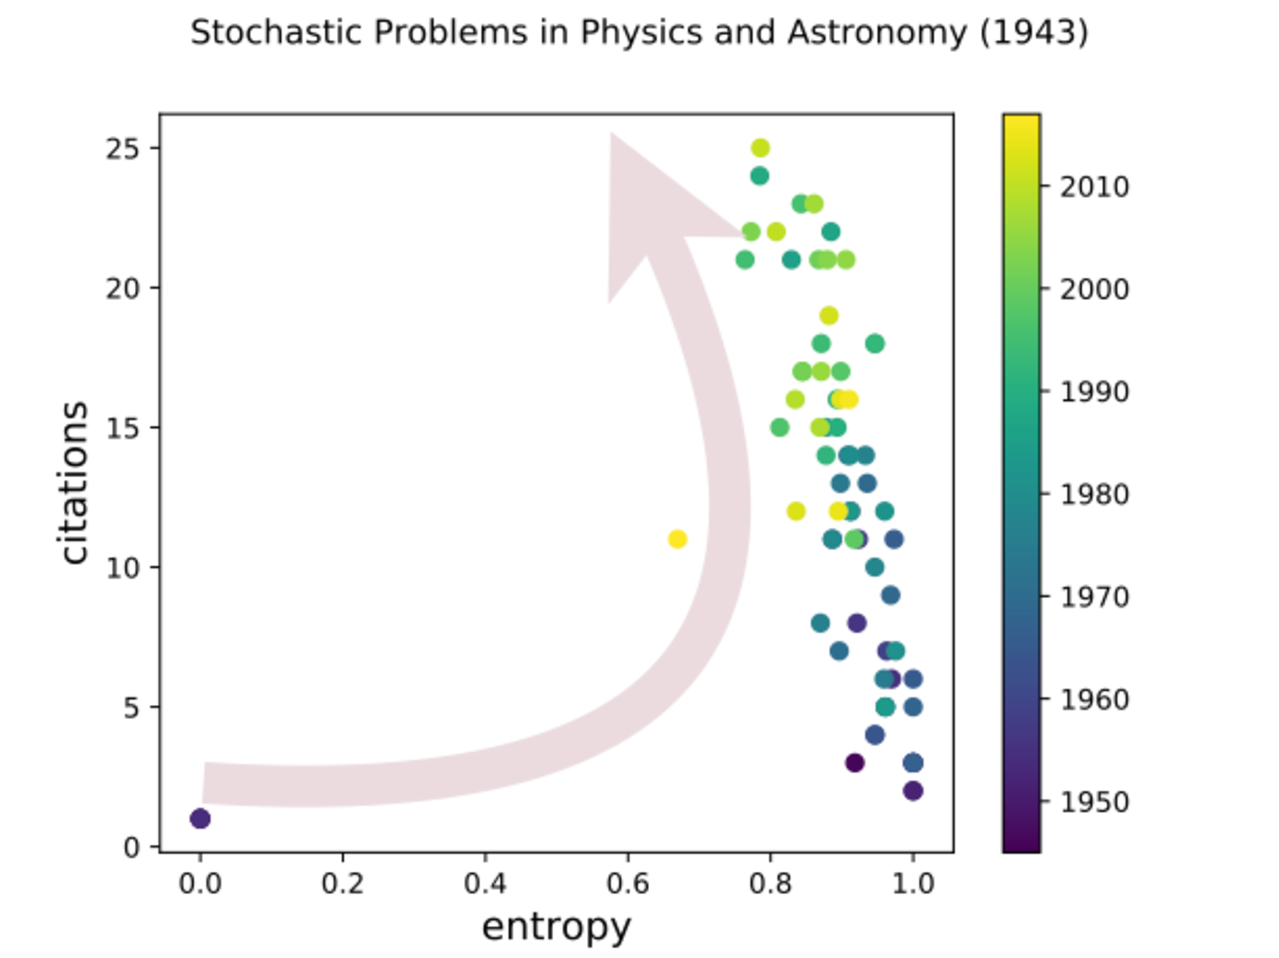
\includegraphics[width=0.42\textwidth]{figures_exaptation/review-entropy.pdf}%
  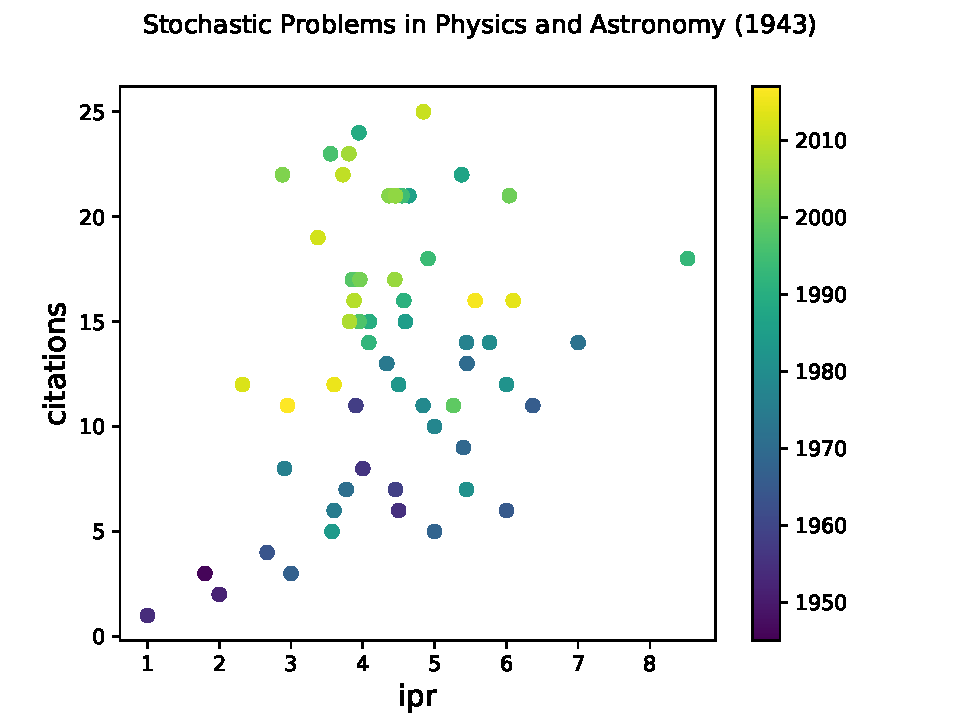
\includegraphics[width=0.42\textwidth]{figures_exaptation/review-ipr.pdf}
\caption{FNE and IPR pattern for a typical review article in APS. Review articles exhibit a distinctive dynamical behaviour slightly different than the exaptation patterns discussed in Figs. 3. and 5. Left: the forward normalised entropy increases quickly and remains at high values over time, while the number of citations per year grows. Right:  the number of clusters citing a review article grows over time showing an increased interest in several sub-disciplines.}
  \label{fig:review}
\end{figure}

\section{Discussion}
The concept of exaptation has not been appropriately quantified. 
Only very few systematic quantitative analyses are available in the literature. 
Here we focused on the exaptation phenomena in the framework of scientific progress as it can be observed in the APS article collection database. 
Our approach consists of looking for signatures of exaptation in the adoption (as reflected in citation patterns) of specific results by other scientific communities than the original scientific area of belonging. 
To make the analysis quantitative, we propose a method based on two main components: clustering of publications based on citation relations, and two observables, the Forward Normalised Entropy (FNE) and the Inverse Participation Ratio (IPR). 
These measures allow to single out patterns that are related to the exaptation phenomena in scientific evolution. 

The evolution of feathers is a classical example of exaptation. 
Feathers were initially adapted to protect against thermal excursions and were later co-opted for flying. 
As soon as birds learn to fly, their fitness improves since they have higher chances of surviving predators. 
We extend this reasoning with a thought experiment ({\em Gedankenexperiment}) to the exaptation of scientific knowledge, where citations represent the fitness and the inverse participation ratio represents the number of  functions a publication acquires over time.

The  example of graphene constitutes a popular instance of exaptation in physics, particularly in contributing to the development of two related sub-fields, electronic structure properties, and graphene. 
It shows that the `survival' of a field depends on how pre-existing concepts are re-used or applied by communities in new domains resulting in new functionalities. 

These results should be seen as preliminary steps towards a quantitative theory of exaptation; they show that is in principle possible to quantify exaptation, once it becomes possible to get a quantitative handle on the evolving context of a field. A better theory of exaptation is necessary to explain how something emerges and evolves by exploring its \emph{creative potential}~\cite{andriani2016exaptation}. 
The creative potential has been described as the functional shift of a particular component that could open up an evolutionary path different from its original and perhaps intentional trajectory~\cite{andriani2016exaptation,kauffman1993origins}. We think that this chapter could stimulate a new wave of studies in this promising area of scientific research. 


% ========================= CHAPTERS ======================================	
\chapter{Forgetting: The lifespan of scientific knowledge}
As explained in the previous chapter, scientific work usually builds on pre-existing knowledge, which is typically acknowledged through citations in publications. Only a small fraction of this knowledge is actively accessed and cited \cite{Meho_2007}. Most works become outdated quickly, are never looked at, are forgotten and  never mentioned again. This is especially true for the increasing number of non-reproducible papers that do not contribute knowledge sustainably~\cite{Loken2017, Ioannidis2005}. On the other hand, there are scientific milestone papers -- typically exceptional works -- that continue to attract citations, even after decades~\cite{Redner2005}. What emerges from the process of knowledge creation, selection, and forgetting is a ``living'' or active body of knowledge  that is actively used -- ideally -- for pushing the scientific frontier forward. The active knowledge is a tiny subset of all the existing knowledge stored in papers. Here, we estimated the  ``active'' body of knowledge in terms of its ``usability'' using citation data. 

Large-scale publication and citation data has become increasingly available in recent years. It opens up the possibility to reconstruct the history of science (production and reception) on the granular basis of individual publications. In particular, it becomes possible to trace citations in so-called citation networks.

There are different types of citation networks. In its simplest form, a citation network, $M_{ij}$, captures which paper $j$ cites paper $i$. If paper $j$ cites paper $i$ then $M_{ij} = 1$, otherwise $M_{ij} = 0$. These networks should not be confused with other popular citation based networks such as the co-citation network or the bibliographic coupling network. The co-citation network, $C_{ij} = MM^T$, contains the information of how often papers $i$ and $j$ appear {\em together} in the reference list of another paper \cite{Small1973}. $C_{ij}=2$ means that there exist two papers that cite both, $i$ and $j$. The bibliographic coupling network, $B_{ij} = M^TM$, on the other hand, states how many references papers $i$ and $j$ have in common \cite{MARTYN1964}. Every paper, $i$, is uniquely associated with a publication date, $t_i$, which makes it possible to bring in the time component of citations. 

There are immediate lessons that have been learned from citation networks that are important in our context. Early contributions date back to the 1960s \cite{deSollaPrice1965} where citation networks were pioneered by investigating links between scientific publications. Along with other insights, most strikingly it was noted, that the percentage of papers receiving $n$ citations in any year approximately scales as a power law in citations $n$. It follows that most papers receive a small number of citations, while a few papers in the ''fat tail'' of the distribution receive many. This observation has been confirmed~\cite{seglen1992, Redner1998}. In follow-up work, an explanation was offered in terms of ''cumulative advantage''~\cite{Price1976}, stating that the probability for a paper to get cited is proportional to the number of citations it accumulated up to that point in time. This process is also called \textit{preferential attachment (PA)}~\cite{Barabsi1999x}. It has been studied in depth and confirmed by a growing number of authors, both in a theoretical context and in the context of citation networks~\cite{Krapivsky2001, Dorogovtsev2002, Albert2002, Newman2003-x, Newman2001, Capocci2006, Jeong_2003}.

While preferential attachment is a plausible mechanism for understanding the structure of citation networks, recent studies suggest that preferential attachment alone does not result in accurate predictions of several features of citation networks~\cite{Borner2004, Lehmann2005}. Other factors need to be taken into account. Timing of publication has been found to be a contributing factor and a first-mover advantage was proposed along with preferential attachment~\cite{Newman2009x}. If a work is among the first in an emerging field, then there is not much competition, and it may receive more citations. It was noted that papers that receive citations unusually quickly tend to continue to receive more citations than usual, even though they might not be the most cited papers at the time~\cite{Newman_2014x}. 

Time not only plays a role in the success of a paper, but also in its ``decline''. In this context, the notion of ``half-life of literature'' has been introduced some time ago~\cite{Burton1960}. It is defined as the time during which the second half of all papers that are still being cited were published. This time is rather short, because most papers cite the recent past~\cite{Burton1960}. This fact was also observed in~\cite{deSollaPrice1965, Redner2005}. In contrast to the  half-life of nuclei, the ``half-life of literature'' is not a constant, but depends on the overall growth of the citation network. For that reason, citation networks must always be considered against the exponential growth of the number of publications. In physics, this growth is characterized by a doubling time of about 11.8 years~\cite{Martin2013}. In ~\cite{Martin2013, Fanelli2016} it is noted that the number of publications per author (productivity) has practically not increased during the last century while the average number of authors per paper has increased~\cite{Martin2013}. The observed growth in the number of publications can therefore be largely attributed to the growth in the overall number of scientists and research funding. From the existence of a half-life of literature and the growth of the network follows, immediately, that the distribution of the age of citations (time between the publication of the citing and the cited paper) is highly skewed towards more recent papers. 
This general trend also persists if one accounts for the exponential growth of the number of articles published each year~\cite{Redner2005}. For this reason it is apparent, that there is a strong preference of papers to cite more recent works, an effect that is often referred to as \textit{aging}~\cite{Wang2013x, Yin2017}.

Preferential attachment in combination with aging are the two mechanisms that form the basis for a number of mathematical models that reasonably explain citation networks and their dynamics. In~\cite{Dorogovtsev2000}, an evolving network model with preferential attachment and a power law aging of nodes is considered. It demonstrates a strong first mover advantage. Another model with preferential attachment and power-law aging~\cite{Safdari2016} shows that if aging is included in the model, the associated degree distribution of the resulting network deviates from a strict power law. They confirm their findings on a Hollywood actor network. In~\cite{Borner2004} an author-paper network is simulated, where authors can read, write, and cite papers, and search for references in a recursive manner. Aging is included by fitting a Weibull distribution to the time-dependent attachment probability of papers. This model explains the deviations from strict power laws in the degree distribution and is supported by empirical data from PNAS articles. A stochastic model of citation dynamics that builds on~\cite{Borner2004} combines preferential attachment and aging with a recursive search and copy mechanism~\cite{Golosovsky2017}. The main result is a non-linearity in the network growth that allows for individual papers to achieve diverging citation trajectories.  The rate at which both, patents and scientific articles, acquire citations is studied in~\cite{Higham2017, Higham2017_2}. There, this rate is modeled with power law preferential attachment and exponential aging. Strikingly, in this model, the aging component is completely independent of the preferential attachment.  Yet another model for patent citation networks assumes the probability to cite a patent to follow linear preferential attachment, as well as power law forgetting with an exponential cutoff~\cite{Valverde2007}. It presents a method to determine this probability from empirical data and shows that the scaling behavior can be explained by the combination of preferential attachment and aging. In all the mentioned models, preferential attachment and aging have an impact on the fate of a paper. Some models allow for short-term performance predictions (citations)~\cite{Newman_2014x, Golosovsky2017, Higham2017_2}; some also do  predictions on longer horizons~\cite{Wang2013x} of individual papers. 

What has been studied in much less detail is the dynamics of scientific work being forgotten. For how long is scientific work relevant?  How long will it take before today’s work is forgotten? Which works have the potential to become milestones, and under what conditions does this happen? Can these conditions be identified by seeing papers not in isolation, but as a part of the citation network? 
What has been missing in this context so far is a model that focuses on the forgetting aspect in the context of a growing citation network. We want to add that missing piece to understand the dynamics of forgetting in order to better estimate the future state of the system as a whole. From that, we can then understand how certain papers stay relevant for  decades, while most papers are forgotten.

\section{A quantitative framework for the forgetting mechanism}

To understand the forgetting process more quantitatively, we introduce a variable to represent the total number of citations originating from papers published in year $i$ that cite papers published in year $j$,
\begin{equation}
c_{t_i t_j} \equiv \sum_{k,l} 
\begin{cases}
M_{kl}, & \text{ if publication year of $k$} = t_j \\
& \text{ and publication year of $l$} = t_i,\\
0 & \text{ else}
\end{cases};
\end{equation}
This is shown in Fig.~\ref{fig:aor}, where each dot represents a paper published in a particular year and each arrow represents a citation from one paper to another.


In Fig.~\ref{fig:aor2} (a) the values of $c_{t_i=2015,t_j}$ (citations per year from papers published in 2015) are shown (blue) for all American Physical Society journals that include about 600,000 papers published between 1893 and 2015 and around 5,000,000 citations. Next, we look at a hypothetical situation, where all papers have the same probability of being cited, independent of their age.
We call the corresponding variable $\overline{c}_{t_it_j}$ (red dashed line).

It is given by $\overline{c}_{t_it_j} = \frac{N_{t_j}}{N}\sum_{t_j} {c}_{t_it_j} $, where $N_{t_j}$ is the number of papers published in year $t_j$, N is the total number of papers published in all years $N=\sum_{t_j}N_{t_j} $ and the sum represents the total number of references of papers published in year $t_i$.

We can see that $\overline{c}_{t_it_j}$ is directly proportional to the number of papers published in every year and can be used as a normalization factor, to account for the growing number of publications. By dividing $c_{t_i=2015,t_j} / \overline{c}_{t_i=2015,t_j}$, we get a measure that is independent of the number of papers published each year.  We call this resulting curve the ``forgetting curve'' of the APS, shown in Fig.~\ref{fig:aor2} (b). Note a general trend of a strong preference towards citing papers that are not older than ten years. In a randomized scenario, where new publications would cite other publications with equal probability, the forgetting curve would fluctuate around a constant value of 1. For simulation results on $\overline{c}_{t_it_j}$, see ~\hyperref[SI1]{SI 1}.
Note that spikes in the forgetting curve coincide with the publishing years of milestone papers. These heavily cited papers stand out from the bulk of papers and cause the corresponding year to be over-represented. We find that in years, where a milestone paper was published, these papers, while making up only $0.03\%$ of the papers published, attract on average $14\%$ of all citations to papers published in that year. For more details, see~\hyperref[SIM2]{SI 2}.

\begin{figure}[h!]
	\centering
	  
\includegraphics[width=0.6\columnwidth]{figures_aps/1a.png}\\
		\caption{ 
		Number of citations, $c_{t_i,t_j}$, originating from papers published in year $t_i$ and citing papers published in year $t_j$.}
	\label{fig:aor}
\end{figure}

\begin{figure}[h!]
	\centering
	  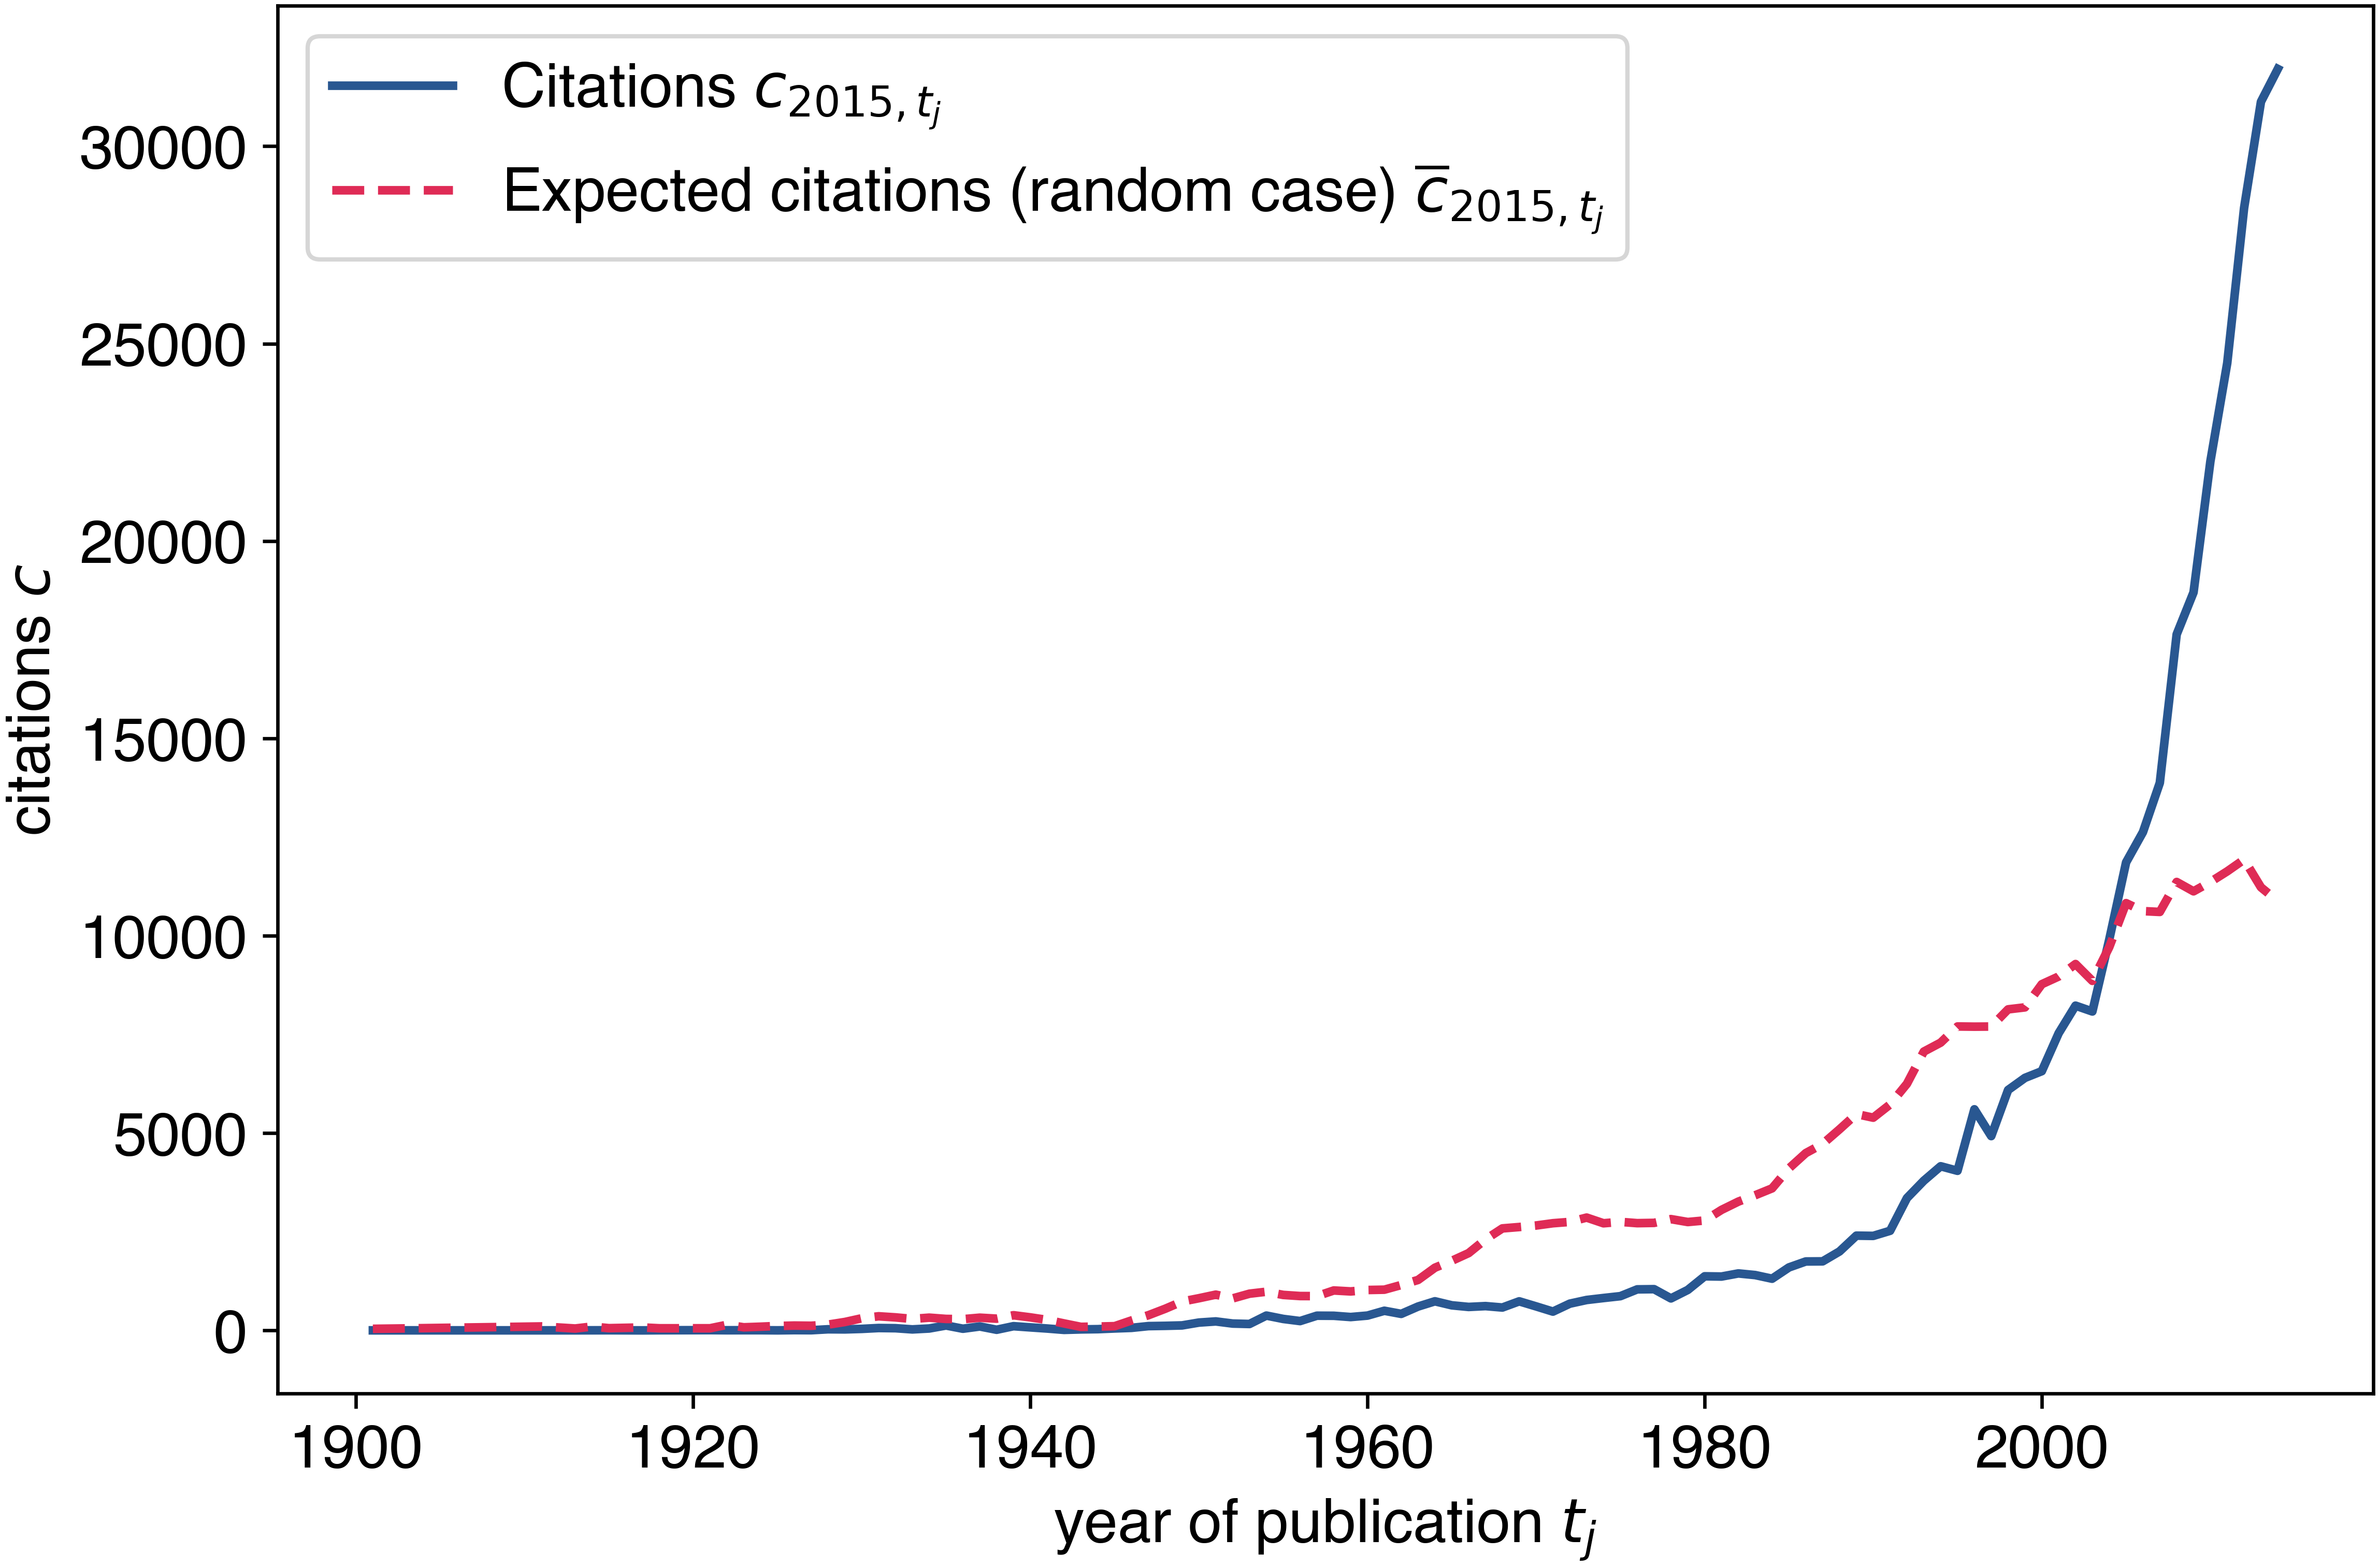
\includegraphics[width=0.6\columnwidth]{figures_aps/1b.png}
	  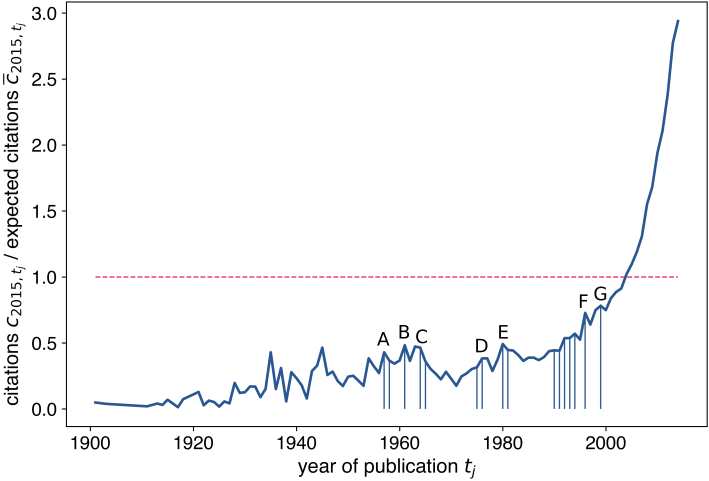
\includegraphics[width=0.6\columnwidth]{figures_aps/1c.png}
		\caption{ 
		(a) Number of citations per year from papers published in 2015 (blue solid line) and expected values of the random case, where citations are assigned to publications randomly with equal probability (red dashed line). The red line is proportional to the number of papers published each year.
		(b) ``Forgetting curve'' or citation preference of papers published in 2015. Values $>1$ indicate a relative preference with respect to equal probability citations, values $<1$ indicate an under-representation.
		Vertical lines mark the publishing years of milestone scientific papers such as:
		A: "Theory of Superconductivity" (Bardeen, Cooper,Schrieffer); B: "Effects of Configuration Interaction on Intensities and Phase Shifts" (Fano); C: "Inhomogeneous Electron Gas" (Hohenberg, Kohn); D: "Special points for Brillouin-zone integrations" (Monkhorst, Pack); E: "Ground State of the Electron Gas by a Stochastic Method"
(Ceperley, Alder); F: "Generalized Gradient Approximation Made Simple" (Perdew, Burke, Ernzerhof) \& "Efficient iterative schemes for ab initio total-energy calculations using a plane-wave basis set" (Kresse, Furthmüller); G: "From ultrasoft pseudopotentials to the projector augmented-wave method" (Kresse, Joubert)}
	\label{fig:aor2}
\end{figure}

The forgetting curve can be used to infer the age structure of the literature new knowledge is built on. We explain the curve with the help of a simple model of citation dynamics that takes into account in different ways the bulk of  publications and the exceptional works. 

To model the dynamical process of citing literature, we devise a simple generative model. We consider the case where a new paper $i$ is published at the time $t_i$ and ask how likely will the paper $i$ cite the paper $j$? To answer it, we measure the function that modulates the  probability of attracting citations for individual publications. This function is based on the age of the referenced paper $j$, $t = t_i - t_j$, and the number of citations the paper $j$ received in the past, up to time $t_i$. We call this function the {\em attachment kernel},  $f(k,t)$. Assuming that the underlying mechanisms of how we choose our references do not change over time, the dependence of $t_i$ and $t_j$ of the attachment kernel can be condensed into one variable $t$. To measure the attachment kernel, we adapt a method used in \cite{Newman2001} and apply it to the 120 years of empirical citation data of the APS; see~\hyperref[SI3]{SI 3}. The resulting kernel can be approximated well by a linear function in $k$ and a power law decay in time,
%
\begin{equation}
   f(k, t)= (k+1)(t+1)^{-\alpha} \quad.
\end{equation}
%
The exponent $\alpha$ cannot be completely decoupled from the number of citations $k$, as it shows a slight dependency $\alpha = \alpha(k) $. However, we show that for the bulk of papers, $\alpha$ can be well approximated as a constant from the empirical data by its mean value over all observations. For the mean, we find a value of $\overline{\alpha} = 1.42$.  We confirm the linear preferential attachment in $k$ found in other works \cite{Jeong_2003}. Here, the offset by 1 represents the finite chance of a publication currently without citations to get cited for the first time. The temporal term represents forgetting.

To this point, the model covers the bulk of average papers. However, as noted before, there are milestone works that are clearly exceptional. These works are causing visible spikes in the forgetting curve Fig.~\ref{fig:aor2} (b) and thus follow a different attachment kernel. If we assume, that the underlying preferential attachment mechanism is the same also for milestones, we can determine their attachment kernel by measuring the value of the exponent $\alpha_m$ of any individual milestone paper $m$. For our analysis, we define milestones as the top thirty most cited papers in the APS, excluding review papers. For each of these papers, we measure the exponent $\alpha_m$ based on the waiting times between events, where these papers receive citations. For details, see~\hyperref[SIM4]{SI 4}. The attachment kernel for milestones has the form:
%
\begin{equation}
   f(k, t, \alpha_m)= (k+1)(t+1)^{-\alpha_m} \quad,
\end{equation}
where $\alpha_m$ can be different for every individual milestone, $m$.

With these ingredients, we can now define the generative model as follows. An exponentially increasing number of papers is published over time. Each of these papers, $i$, cites multiple other papers $j$ that were published before. The probability of $j$ to be cited by $i$ is proportional to the attachment kernel $f(k, t)$, where $k$ is the number of citations that paper $j$ has at that point in time and $t$ is the time difference in years between the publishing times of paper $i$ and paper $j$. To normalize the probability, $f(k,t)$ is calculated for all average papers and  $f(k,t,\alpha)$ for all milestone papers at each point in time. Here, we define milestones as the top thirty most cited papers in the APS, excluding review papers. Following this model, one can generate a simulated citation network.

\section{Results}
\subsection{Null model validation} To test the model, we generate a {\em randomized} citation network that serves as a null model. To generate it, we take the publishing dates and out-degrees of papers from the APS, but omit the information about which paper cites which. The process of citing is replaced by a random process, where probabilities for individual papers to receive a citation are proportional to their respective attachment kernel, $f(k, t)$. We include the publishing dates and individual attachment kernels $f(k, t, \alpha_m)$ for milestones in this model. We then assign the references paper by paper, ordered in time, until we have reconstructed the full citation network. For details, see~\hyperref[SI5]{SI 5}. On the reconstructed network, we measure the forgetting curve. In Fig.~\ref{fig:nullcomparison} the resulting forgetting curve for the null model (red dashed line) is compared to the empirical forgetting curve  (blue solid line) that was introduced in Fig.~\ref{fig:aor2} (b). 

The general features of the null-model are in good agreement with the empirical values, especially for the more recent decades. To assess how far the null model deviates from the empirical data, we calculate the mean absolute percentage error (MAPE) on the forgetting curves. This value is calculated by taking the absolute value of the relative deviation between null model and empirical data for each data point. The resulting values are then averaged to arrive at the MAPE. When comparing the null model to empirical data, the MAPE is below $6\%$ for the last 30 years. It increases for the earlier years, up to values of $35\%$ if the whole 120 years of the APS, including early years with low numbers of publications and high volatility, are taken into account. The low MAPE for recent years implies that the null model accurately reproduces the forgetting curve of the real APS. Note that also some spikes caused by milestone papers are present in the null model. The magnitude of these spikes is captured well for years after the 1990s. For earlier years, low publication numbers are resulting in higher volatility. Nevertheless, the impact of the largest milestones is reflected moderately well, with exception of the year 1935. In this year, a major milestone of physics was published by Einstein, Podolsky and Rosen, which remained almost unnoticed for decades, serving as a prime example of a "sleeping beauty" \cite{Ke2015}. This unusual citation pattern leads to an underestimation of citations in the null model. For more details, see ~\hyperref[SI6]{SI 6}. Overall, the similarity of the null model and the empirical data implies that the attachment kernel was measured accurately and  captures the essential underlying citation dynamics.

\begin{figure}[h!]
	\centering
	  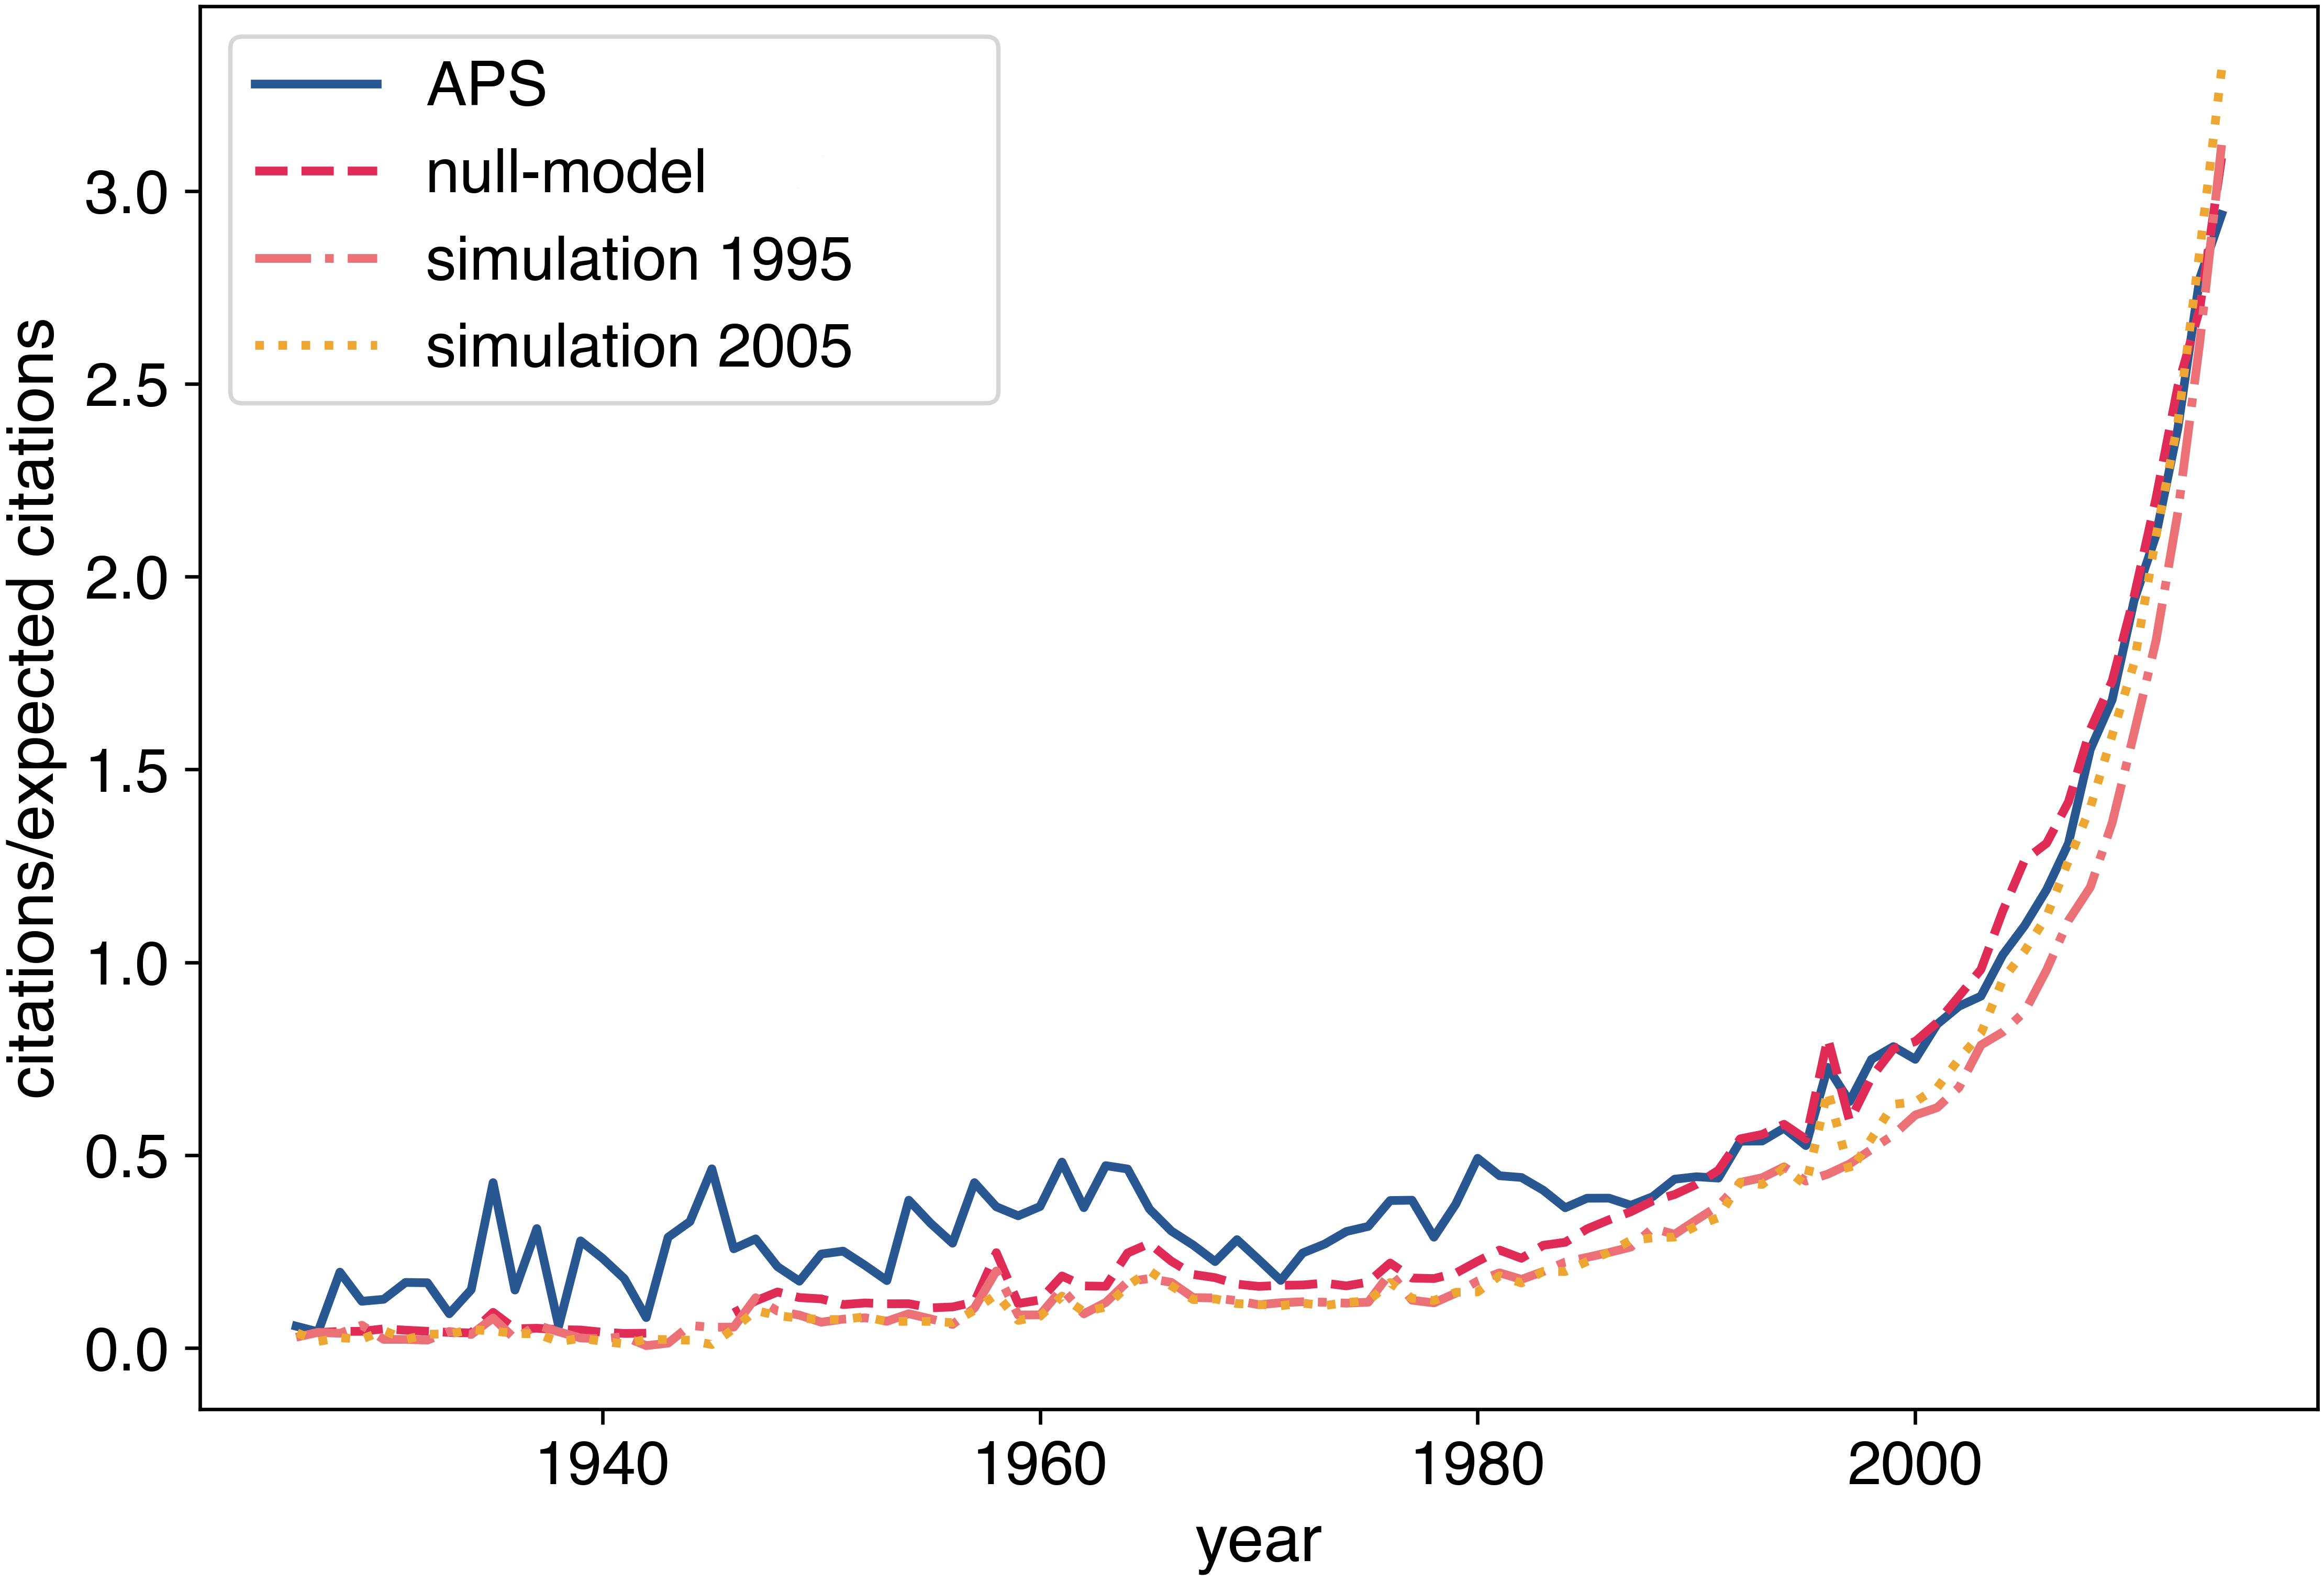
\includegraphics[width=0.7\columnwidth]{figures_aps/2.png}
		\caption{Forgetting curve for the APS citation network for the empirical data (blue), the null model based on attachment kernel $f(k, t)$ (red) and the out-of-sample predictions for the years 1995-2015 (orange) and 2005-2015 (yellow), based on empirical data from 1893 to 1995 and 1893 to 2005 respectively.}
	\label{fig:nullcomparison}
\end{figure}

\subsection{Out-of-sample prediction} Next, we estimate the predictive power of the model by asking if the model can be used to simulate plausible future citation networks. To test the predictive power, we split our empirical data in two parts, separated by age, and try to predict the second part using data only from the first part. The quality of the prediction can then be assessed by comparing the prediction results with the empirical data. The first part consists of all papers published until 1995, the second part that we predict are all papers published between 1995 and 2015. We assume (realistically) that the number of references per paper stays more or less constant and that the number of publications published per year grows exponentially with a rate $\gamma = 0.0587$ corresponding to a doubling time of $11.8$ years as determined in \cite{Martin2013}. For our prediction, we use the attachment kernel that we measured on the full APS citation network using data until 1995 only. We simulate the occurrence of new milestone papers with a Poisson process with exponentially distributed waiting times with an estimated rate $\lambda$ from the empirical data. The simulation works as for the null model, but instead of taking the publishing dates and out-degrees from empirical data, we assume an exponentially increasing stream of publications with a constant number of references. We bootstrap the empirical citation network until 1995 and simulate the next 20 years for the forgetting curve of 2015. We then repeat the process on a shorter time period of ten years, between 2005 and 2015.

For the predicted citation network, we compute the forgetting curve and compare it to the empirical one from the APS, see Fig. \ref{fig:nullcomparison}. The orange line shows the forgetting curve of the simulation. It yields a reasonable  approximation to the empirical forgetting curve (blue line). The MAPE for the last 30 years is around $21\%$. This means, that the last three decades of the forgetting curve we predicted for 2015 based on data up to the year 1995 on average deviates  less than $21\%$ from the empirical forgetting curve. The second prediction, for the years between 2005 and 2015, is shown in yellow. Here, the MAPE for the last 30 years is around $17\%$. If all earlier years, back to the 19th century, are included, the error increases up to values of $50\%$. Note that the absence of a spike in the year 1996 in the orange curve is due to the simulation only using publication data until 1995. 

\subsection{Predicting milestones} We next test the predictive power of the model for milestone papers by asking how predictive the exponent $\alpha_m$ is for a paper becoming a milestone in the future. We first define a set of \emph{potential milestones} as all those papers that had at least 200 citations by the end of  2005, a condition that is matched for 814 papers in the data set. Next, {\em true milestones} are defined as those papers that receive at least 50 citations in the year, 10 years after they received their first 200 citations. At this citation rate  they would be ranked among the top cited papers within a few decades. For each potential milestone, $m$, we measure the exponent, $\alpha_m$, based on the first 200 citations.
If this exponent is small, the forgetting can be over-compensated by the preferential attachment mechanism. Thus, if the measured exponent is below a threshold, $\alpha_m \leq \alpha_c$, we predict that the paper will receive more than 50 citations in one year after ten years.

The predictive power of this binary classifier is seen in the ROC curve in Fig. \ref{fig:roc} (a), where we find an AUC of up to 0.89. The high value for the AUC suggests that $\alpha_m$ is a good predictor of the future success of a paper, with high specificity and sensitivity. While our definition of {\em true milestones} was somewhat arbitrary, we confirm that a wide range of thresholds results in reasonably high AUC values and the choice of threshold thus does not significantly impact our results. Our definition of \emph{potential milestones} is based on the requirement for a high number of data points in order to get a low-variance measurement of the exponent $\alpha_m$. For details, see~\hyperref[SIM4]{SI 4}.
Note that on the left side of the ROC curve in Fig. \ref{fig:roc} (a) there is a convex section that indicates, that there are some papers that initially have a very small  $\alpha_m$ exponent but fail to stay popular in the long run and thus are erroneously classified as milestones in our model. We hypothesize that the convex section is caused by papers with a sudden but brief success -- ''flash in the pan'' papers.   

\begin{figure}[h!]
	\centering
	  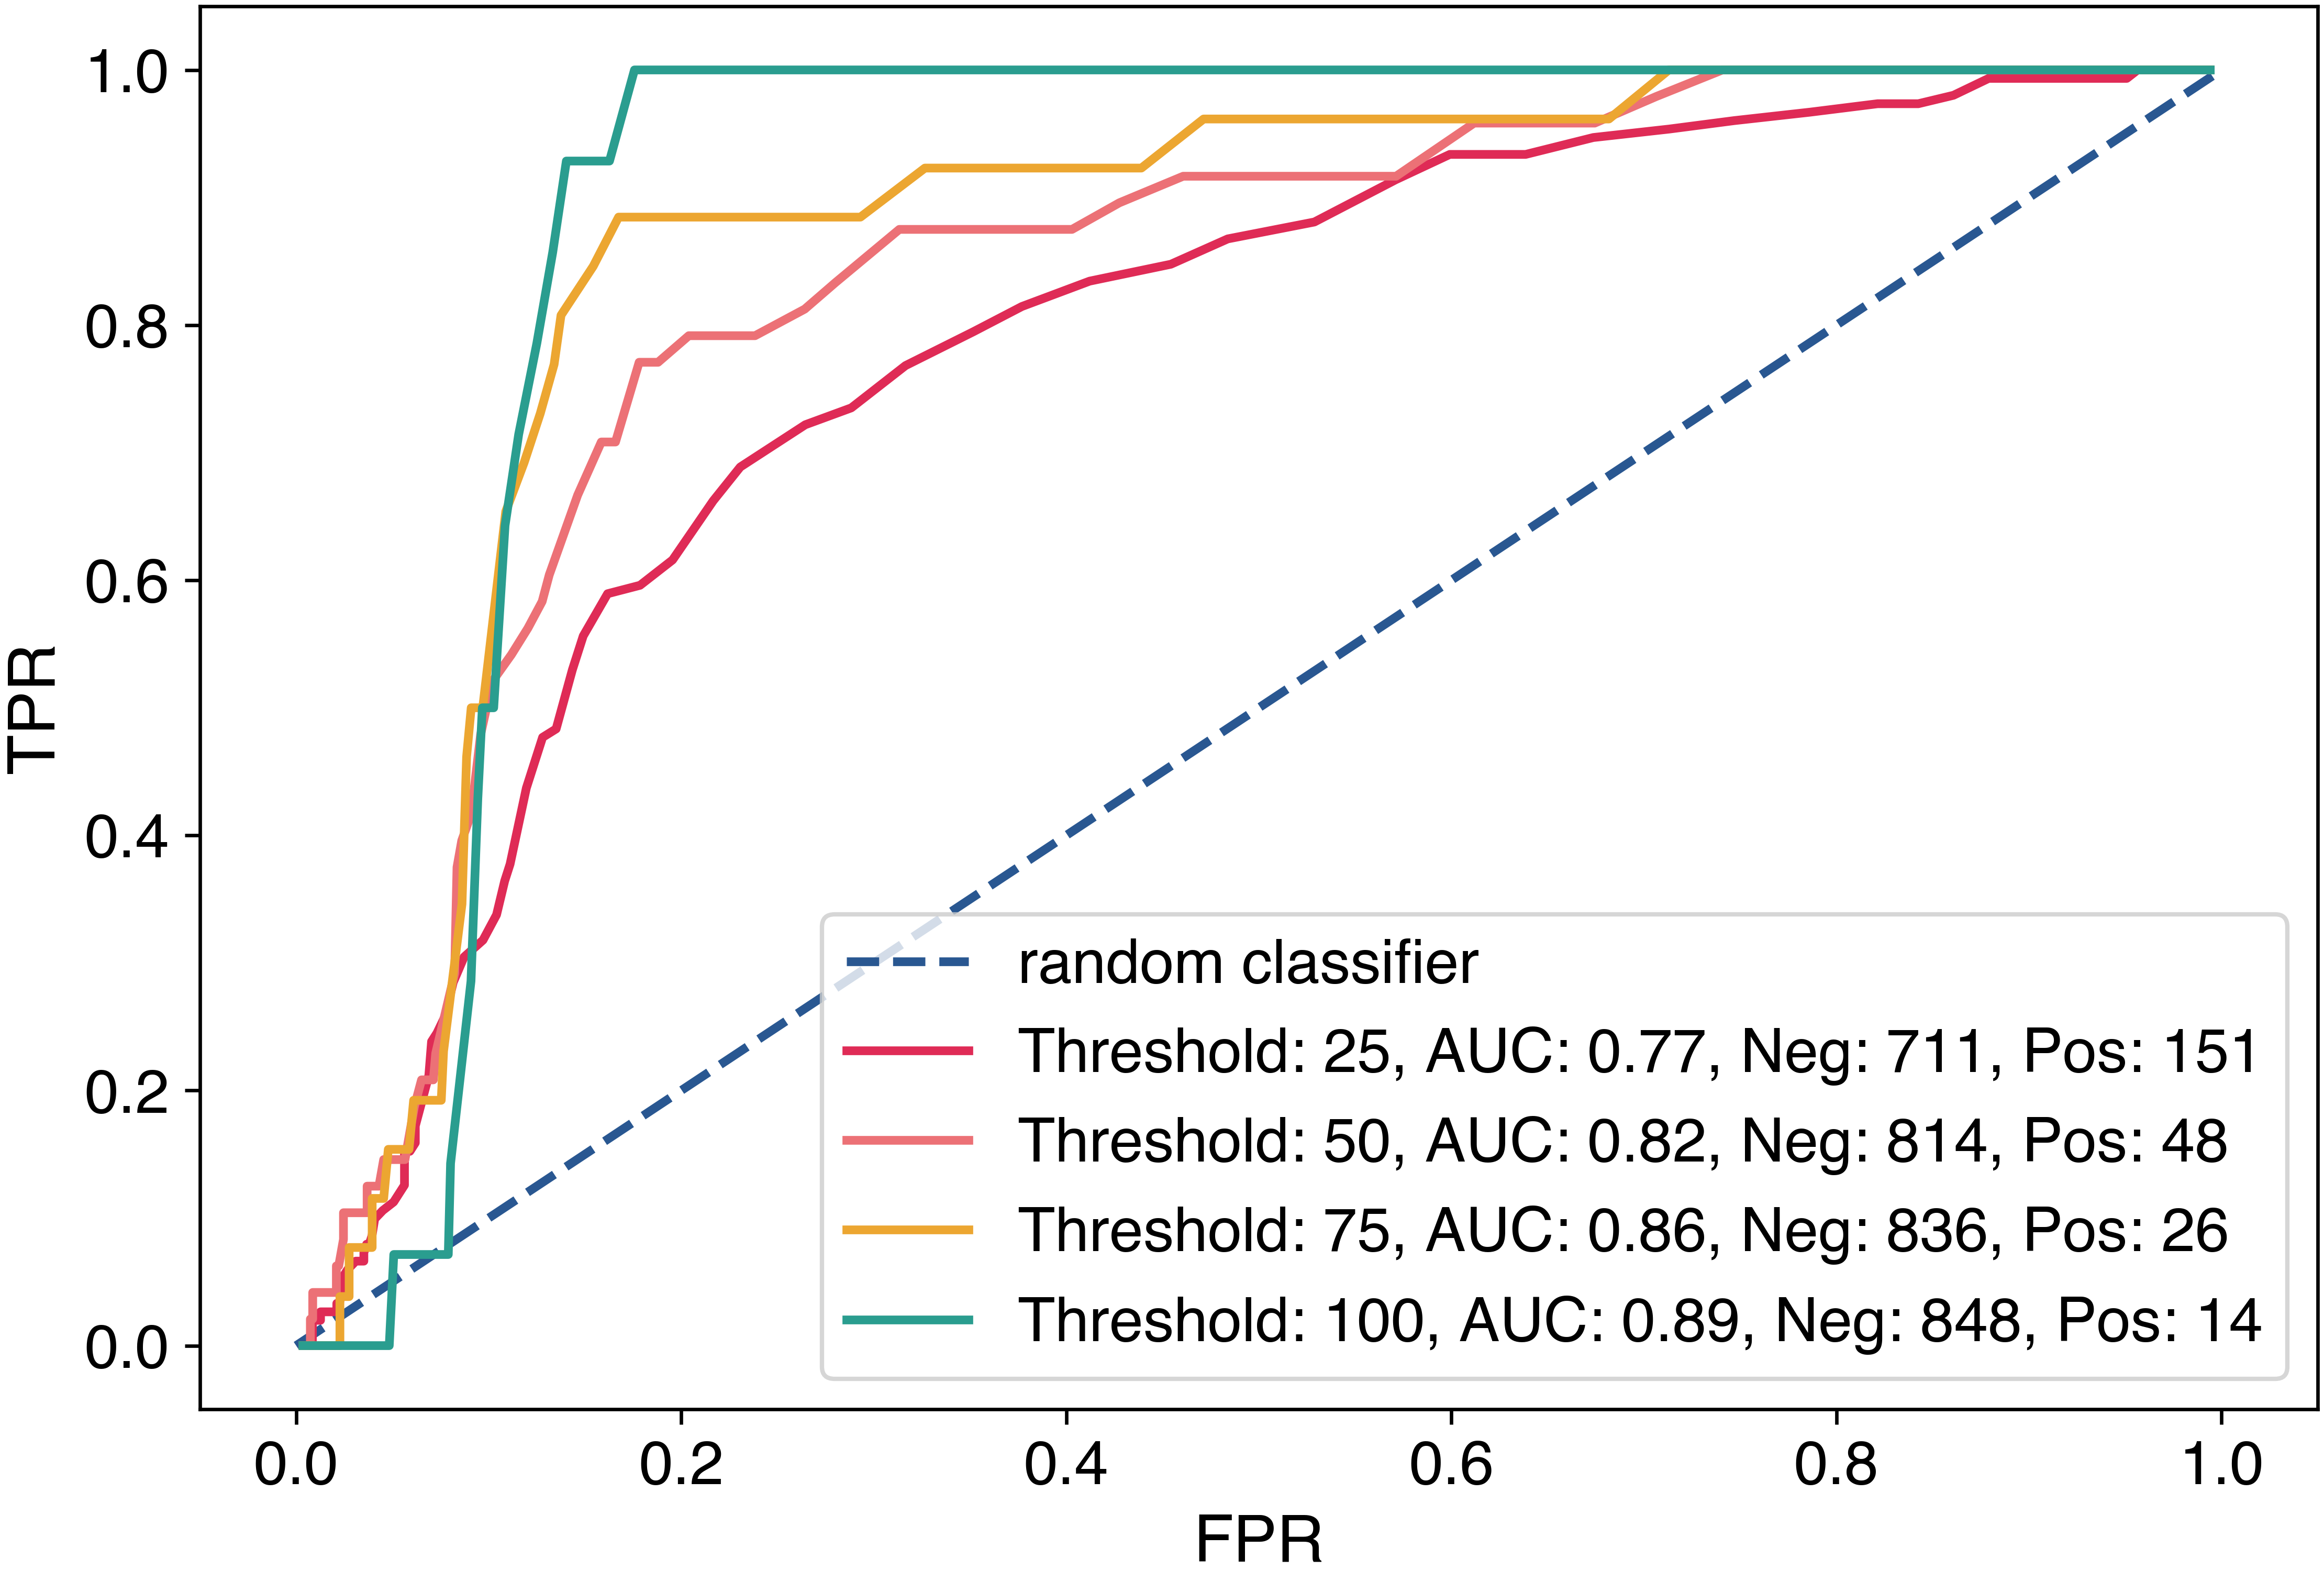
\includegraphics[width=0.7\columnwidth]{figures_aps/6.png}
	  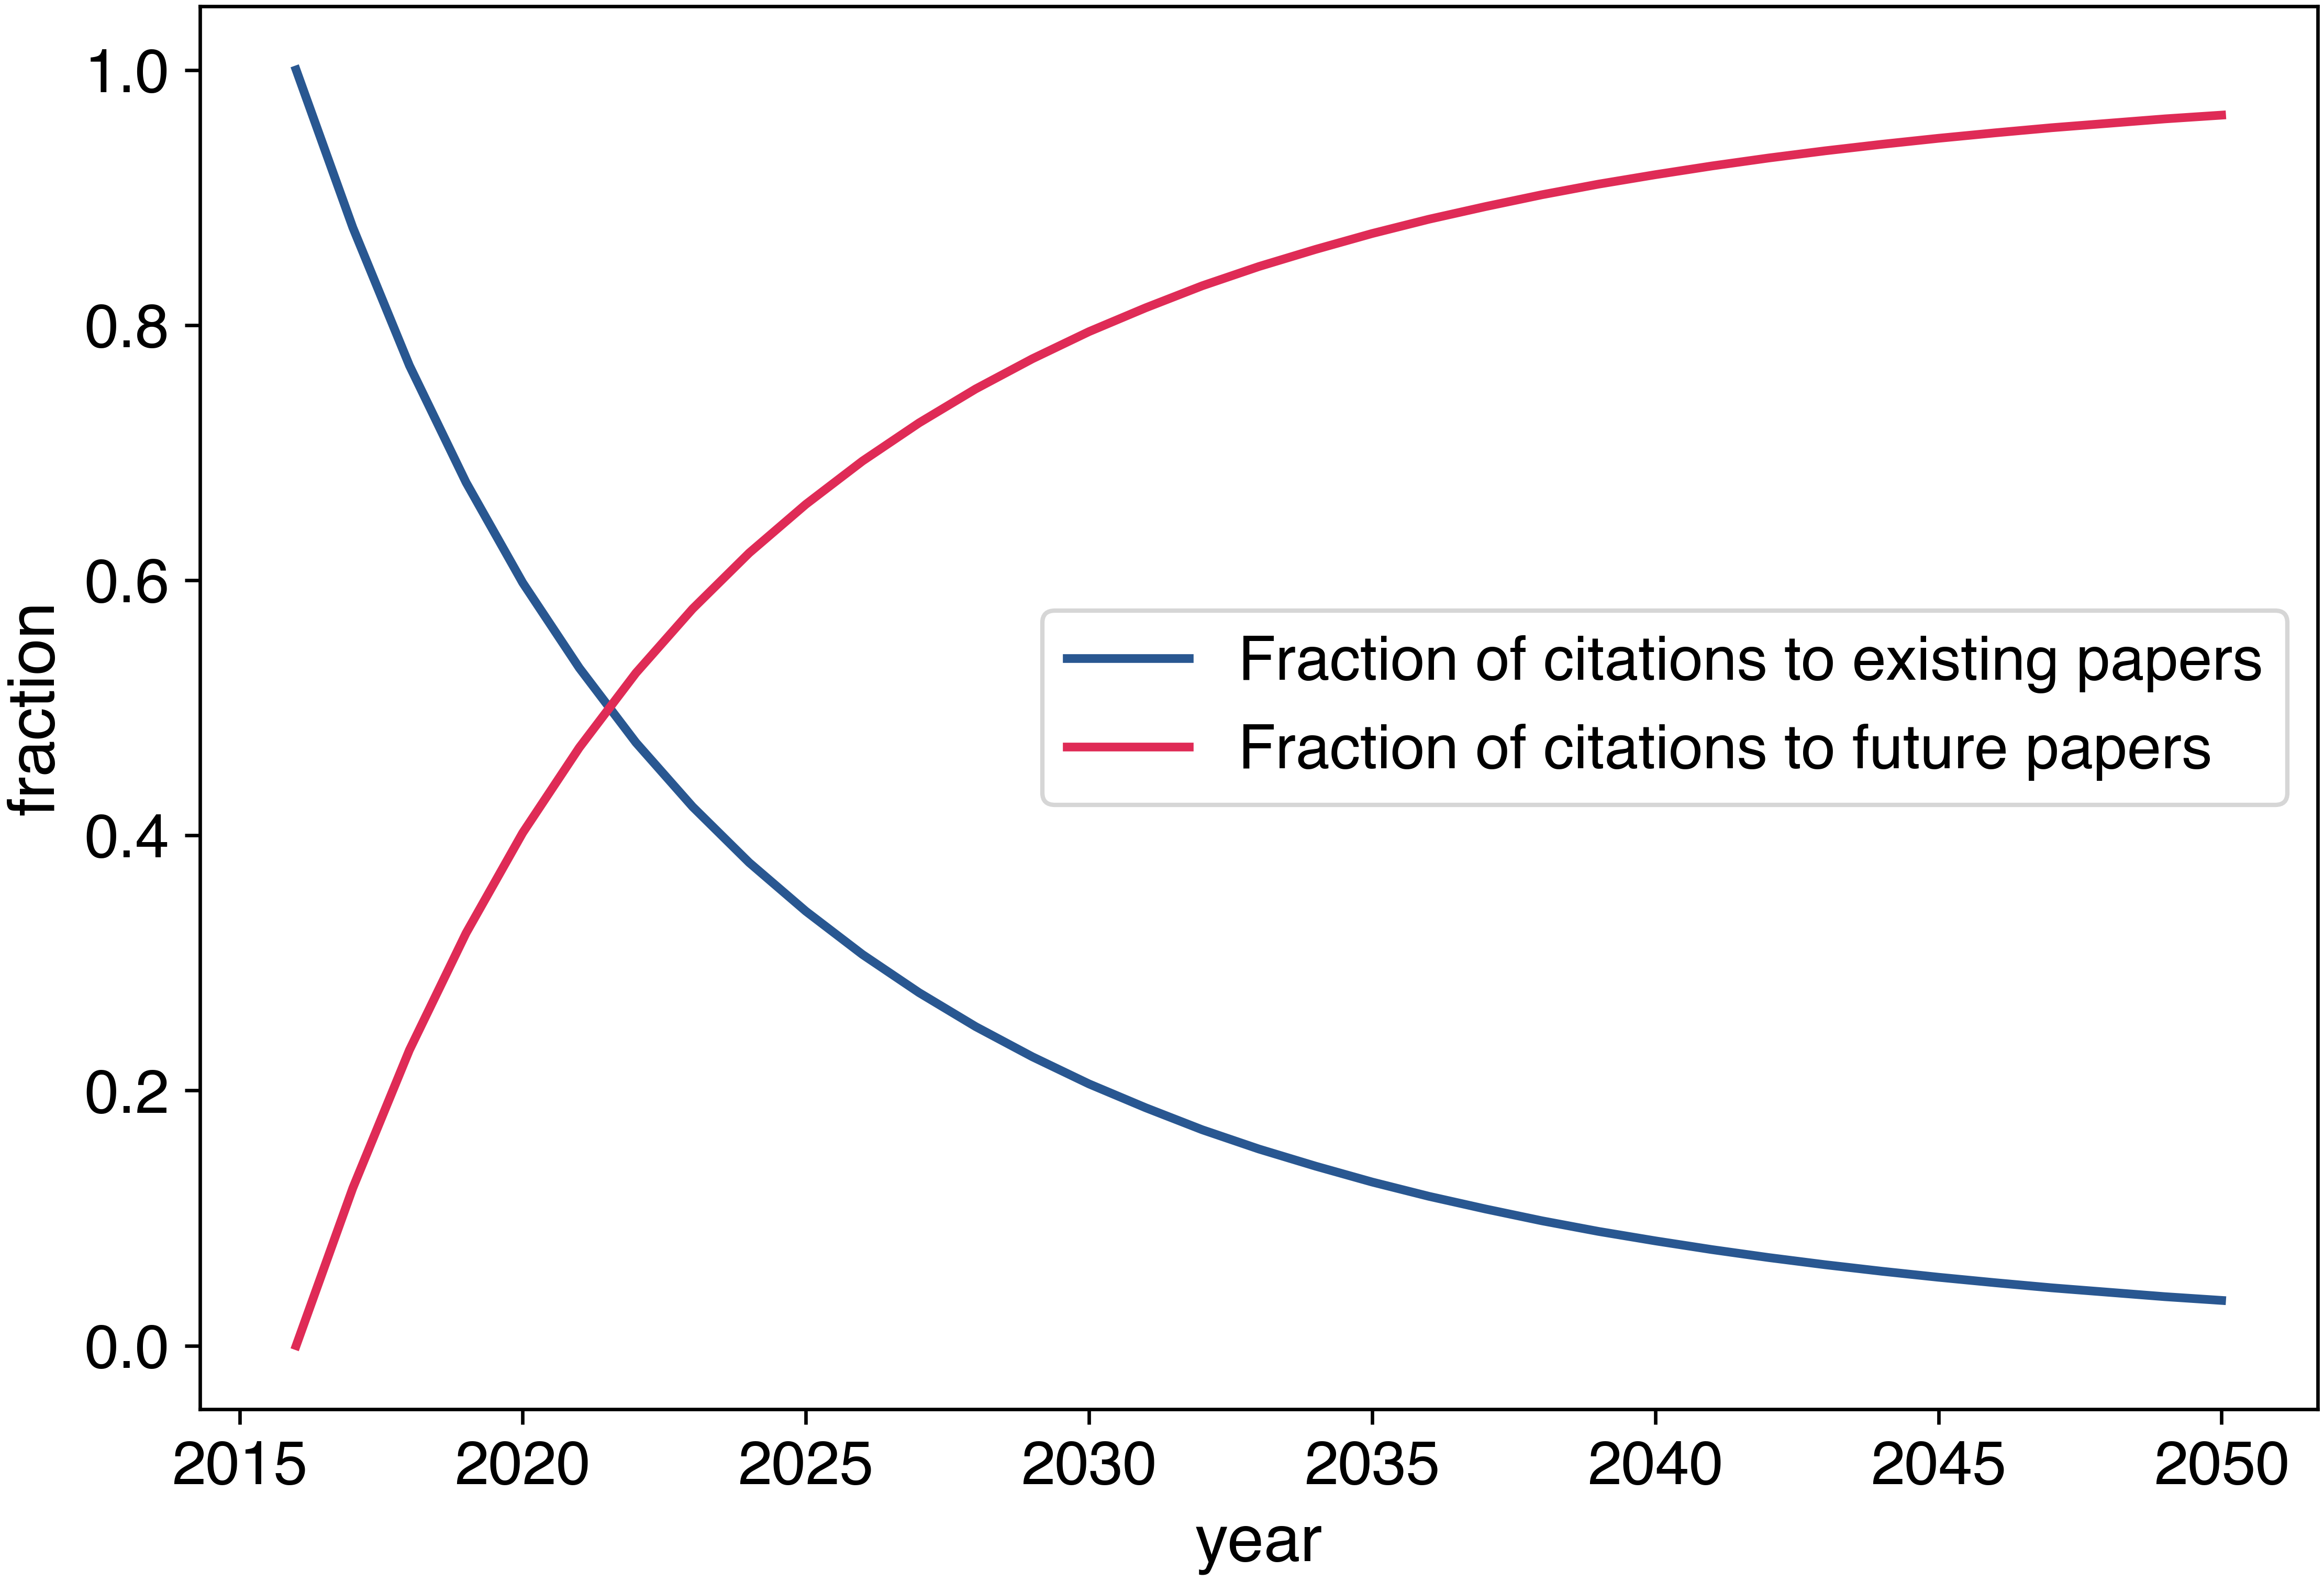
\includegraphics[width=0.7\columnwidth]{figures_aps/3.png}
		\caption{(a) ROC curve (true positive rate vs. false positive rate) for predicting the success of potential milestone papers, $m$, after 10 years, based on their exponent, early in their existence, $\alpha_m$. We show the ROC curves for different thresholds. These thresholds are defined as the minimum number of citations, that a paper must receive in one year, ten years after we measured its exponent $\alpha_m$. The legend shows the values for the area under the curve (AUC) as well as for the number of positives (POS) and negatives (NEG) in our data set for each treshold.
		(b) What we will cite in the future? For every year on the x-axis we consider the references of papers published in that year. The blue curve represents the fraction of references to papers published up to --and including-- 2015. The red curve is the fraction of references to papers, published after 2015. Roughly 20\% of citations from papers published in 2030 are going to papers published until 2015. $96\%$ of the papers cited 30 years from now are not yet written. 
		}
	\label{fig:roc}
\end{figure}

For the prediction, we estimate an individual constant $\alpha_m$ based on the first 200 citations of each potential milestone. If instead of taking the first 200 citations, these exponents $\alpha_m$ are derived from several hundreds of citations, a closer look reveals that many of the exponents come with a positive slope as a function of the number of citations $k$. This indicates that for milestone papers, the attachment kernel cannot be factorized as $f(k,t, \alpha_m)=g(k) h(t, \alpha_m)$. For that reason, if one is interested in predicting citation trajectories of individual papers with more than a few hundred citations, $\alpha_m$ should not be taken as a constant but rather as a function of $k$. We find, that this function is best approximated by a linear function $\alpha_m(k) = \alpha_{m_{0}} + \beta k$, which can be estimated from the data in an analogous way. For details, see~\hyperref[SIM4]{SI 4}.

\subsection{Predicting future citation landscapes}
After confirming that the model accurately predicts the general shape of the forgetting curve, as well as the success of individual papers, we use it to predict what citations today's research will get. We simulate the future citation network as in the situation of the out-of-sample prediction. We bootstrap it on all empirical data until the end of 2015 and then simulate the next 35 years into the future, based on a continued exponential increase of papers and on the attachment kernel measured until 2015. We simulate the network by introducing paper by paper, until we arrive at the possible citation network for the year 2050. Each simulation is performed 10 times and the results are averaged.

From this simulated citation network for the years 2016 to 2050, we estimate how quickly today's work will be forgotten. For each of these years, we define the fraction of citations that go to publications published before --and including-- 2015, which we call \textit{existing papers}. The fraction of citations that go to publications published after 2015 we call \textit{future papers}. Figure \ref{fig:roc} (b) shows that the fraction of citations to \textit{existing papers} decreases to about $30\%$ within ten years into the future and reaches a value of $3.6\%$ in 2050. If we shift the curve by six years to estimate what will happen to papers published in 2021, we conclude that more than $95\%$ of the papers cited in 2050 are not yet written. 

\subsection{Empirical citation trends}
The empirical data of the APS reveals additional trends that are important in our context. First, the average number of citations that papers published in a certain year receive, has been decreasing since the 1960s. And second, larger and larger fractions of our references consist of comparably old and highly cited milestone papers, while the fraction of milestones among the newly published papers has been steadily declining. For details, see~\hyperref[SI7]{SI 7}.

\section{Discussion}
In this chapter, we focused on understanding how scientific work is being utilized or forgotten. In empirical citation networks, we observe two main mechanisms: a linear preferential attachment and a power-law temporal forgetting. We capture these empirical findings in a generative model in which newly published papers cite older papers with a probability proportional to an attachment kernel $f(k, t)$. The kernel reflects two main factors: the cited paper's academic age and the number of citations it already received. This result implies that an article's probability of receiving a citation grows linearly with the citations already received and decays with its publication age as a power-law, characterised by an exponent $\alpha$.

While there is a strong preference towards citing recent papers, some milestone works --potentially of exceptional impact-- continue to attract citations even after decades. These singular milestones, $m$, are characterized by an exponent $\alpha_m < 0.85$. In comparison, the exponent for the bulk of non-exceptionally successful papers is about  $\alpha \sim 1.4 $. Based on $\alpha_m$, one can predict whether a paper will continue to be successful beyond the age of ten years. The corresponding ROC analysis yields an AUC of $0.83$, confirming that the exponent is a good predictor indeed. 

The model reproduces the highly skewed distributions of the number of citations and the age of references observed in other works. In particular, the forgetting curve that results from the model shows a strong tendency to cite recent papers~\cite{deSollaPrice1965, Burton1960}, while older papers fade progressively in oblivion~\cite{deSollaPrice1965, Redner2005, Burton1960}. The spikes observed in the forgetting curve highlight the impact of milestone papers that are remembered for a long time~\cite{Redner2005, Golosovsky2017}.

The linear preferential attachment mechanism in our model confirms the linear dependence on the number of citations, originally found in ~\cite{Jeong_2003}. The second mechanism we find is power-law-like forgetting. While forgetting, or aging, is a mechanism found in most models of citation dynamics, its detailed functional description remained controversial~\cite{Yin2017, Borner2004, Dorogovtsev2000, Valverde2007, Higham2017_2, Safdari2016, Golosovsky2017}. In~\cite{Borner2004} an author-paper network yields an attachment kernel with an aging component that follows a Weibull distribution. \cite{Golosovsky2017, Higham2017_2} both investigate the citation rate of individual papers and find exponential aging, while~\cite{Valverde2007} studies a patent citation network and finds power-law aging with an exponential cutoff in {\em intrinsic time}, where each new patent represents one timestep~\cite{Safdari2016, Dorogovtsev2000},  both find power-law aging in intrinsic time. \cite{Dorogovtsev2000} applies it to the context of citation networks while~\cite{Safdari2016} applies it to a Hollywood-actor network. In~\cite{Lefortier}, the attachment kernel of online media content is described by a model based on preferential attachment, modulated by an exponential forgetting, for which exponents are experimentally determined from data.
Our model finds a power-law-like forgetting mechanism with an exponent larger than one for the bulk of average papers. For milestone scientific papers, we find values below one. Power-law-like forgetting implies that papers are forgotten relatively quickly and only have a limited time to attract attention. However, power laws also indicate that old papers keep a chance to get cited. This result enables a few notable publications that attracted much attention early on to continue attracting citations for a long time. 

There are several limitations to our model. In particular, it relies on the assumption that the way scientific literature evolves will not change fundamentally. This includes the assumption that the scientific output continues to grow exponentially, an assumption that might not hold forever~\cite{Brown2011}. This observation limits the prediction of the number of citations a paper will receive in the future, simply because the total number of citations is directly proportional to the number of articles published. However, our results only partially depend on this assumption, as the general shape of the forgetting curve is also recovered well for sub-exponential growth and even for linear growth. On the other hand, our model also assumes no fundamental changes in how citations are chosen. This assumption might not hold if, for instance, disruptive new technologies are introduced and adopted globally, as had been the case with the internet.

To forecast citation trajectories of individual highly cited papers, our model provides a simple indicator based only on the citation network. For higher accuracy, additional parameters, such as the popularity of the authors, the size of the field, or the novelty of the publication, should be taken into account~\cite{ST2020, Klimek2016, Newman2009x, Martin2013, Newman_2014x, Acuna2012, Shen2014, Sinatra2016, Wang2013}. However, even taking these factors into account, there remains uncertainty due to unpredictable events such as a highly relevant discovery that went unnoticed for a while, termed ``sleeping beauty'' ~\cite{vanRaan2004} or the rediscovery of a paper outside its original domain, called exaptation~\cite{ferreira2020}.

Restricting our model to only age and number of citations makes it easily transferable to other domains. The possiblity that the life-cycle of scientific literature might be different in physics than for other fields like biology, medicine, or philosophy, and even in non-scientific domains such as the music and entertainment industry, is an interesting research direction.

Finally, our model allows for projecting the current citation ecosystem into the future and investigating its sustainability. Through the empirical forgetting kernel, and under the assumption that the number of papers will keep growing exponentially, it is possible to simulate possible future citation networks. For instance, one learns that 95\% of today's (and yesterday's) work will be outdated before the end of the next three decades. It is this finding, and the fact that papers are receiving fewer and fewer citations on average and have decreasing chances of becoming a milestone, that has substantial implications both for individuals and for scientific policies. Partially, the observed dynamics might be attributed to an increasing fragmentation in the system, driven by the emergence of sub-fields. The fragmentation becomes evident, if one looks at the increase in the number of journals in the APS over the last decades. In this fragmented system, papers might become isolated inside of sub-fields and reach smaller scientific audiences on average. On the other hand, a much more worrisome interpretation of our findings hints towards an increasing quantity-over-quality dynamic, where increasingly short lived publications receive little attention and have diminishing chances of becoming works of great impact.

\newpage

\section{Supplementary information}
\setcounter{page}{1}

\subsection{Forgetting curve in the random case}
\label{SI1}

The forgetting curve can fluctuate around a value of 1 if each paper had the same probability of getting cited. The result of a simulation implementing this simple random model is shown in figure \ref{fig:si1}. The curve results from averaging the results of 20 independent simulation runs.


\begin{figure}[!ht]
	\centering
	 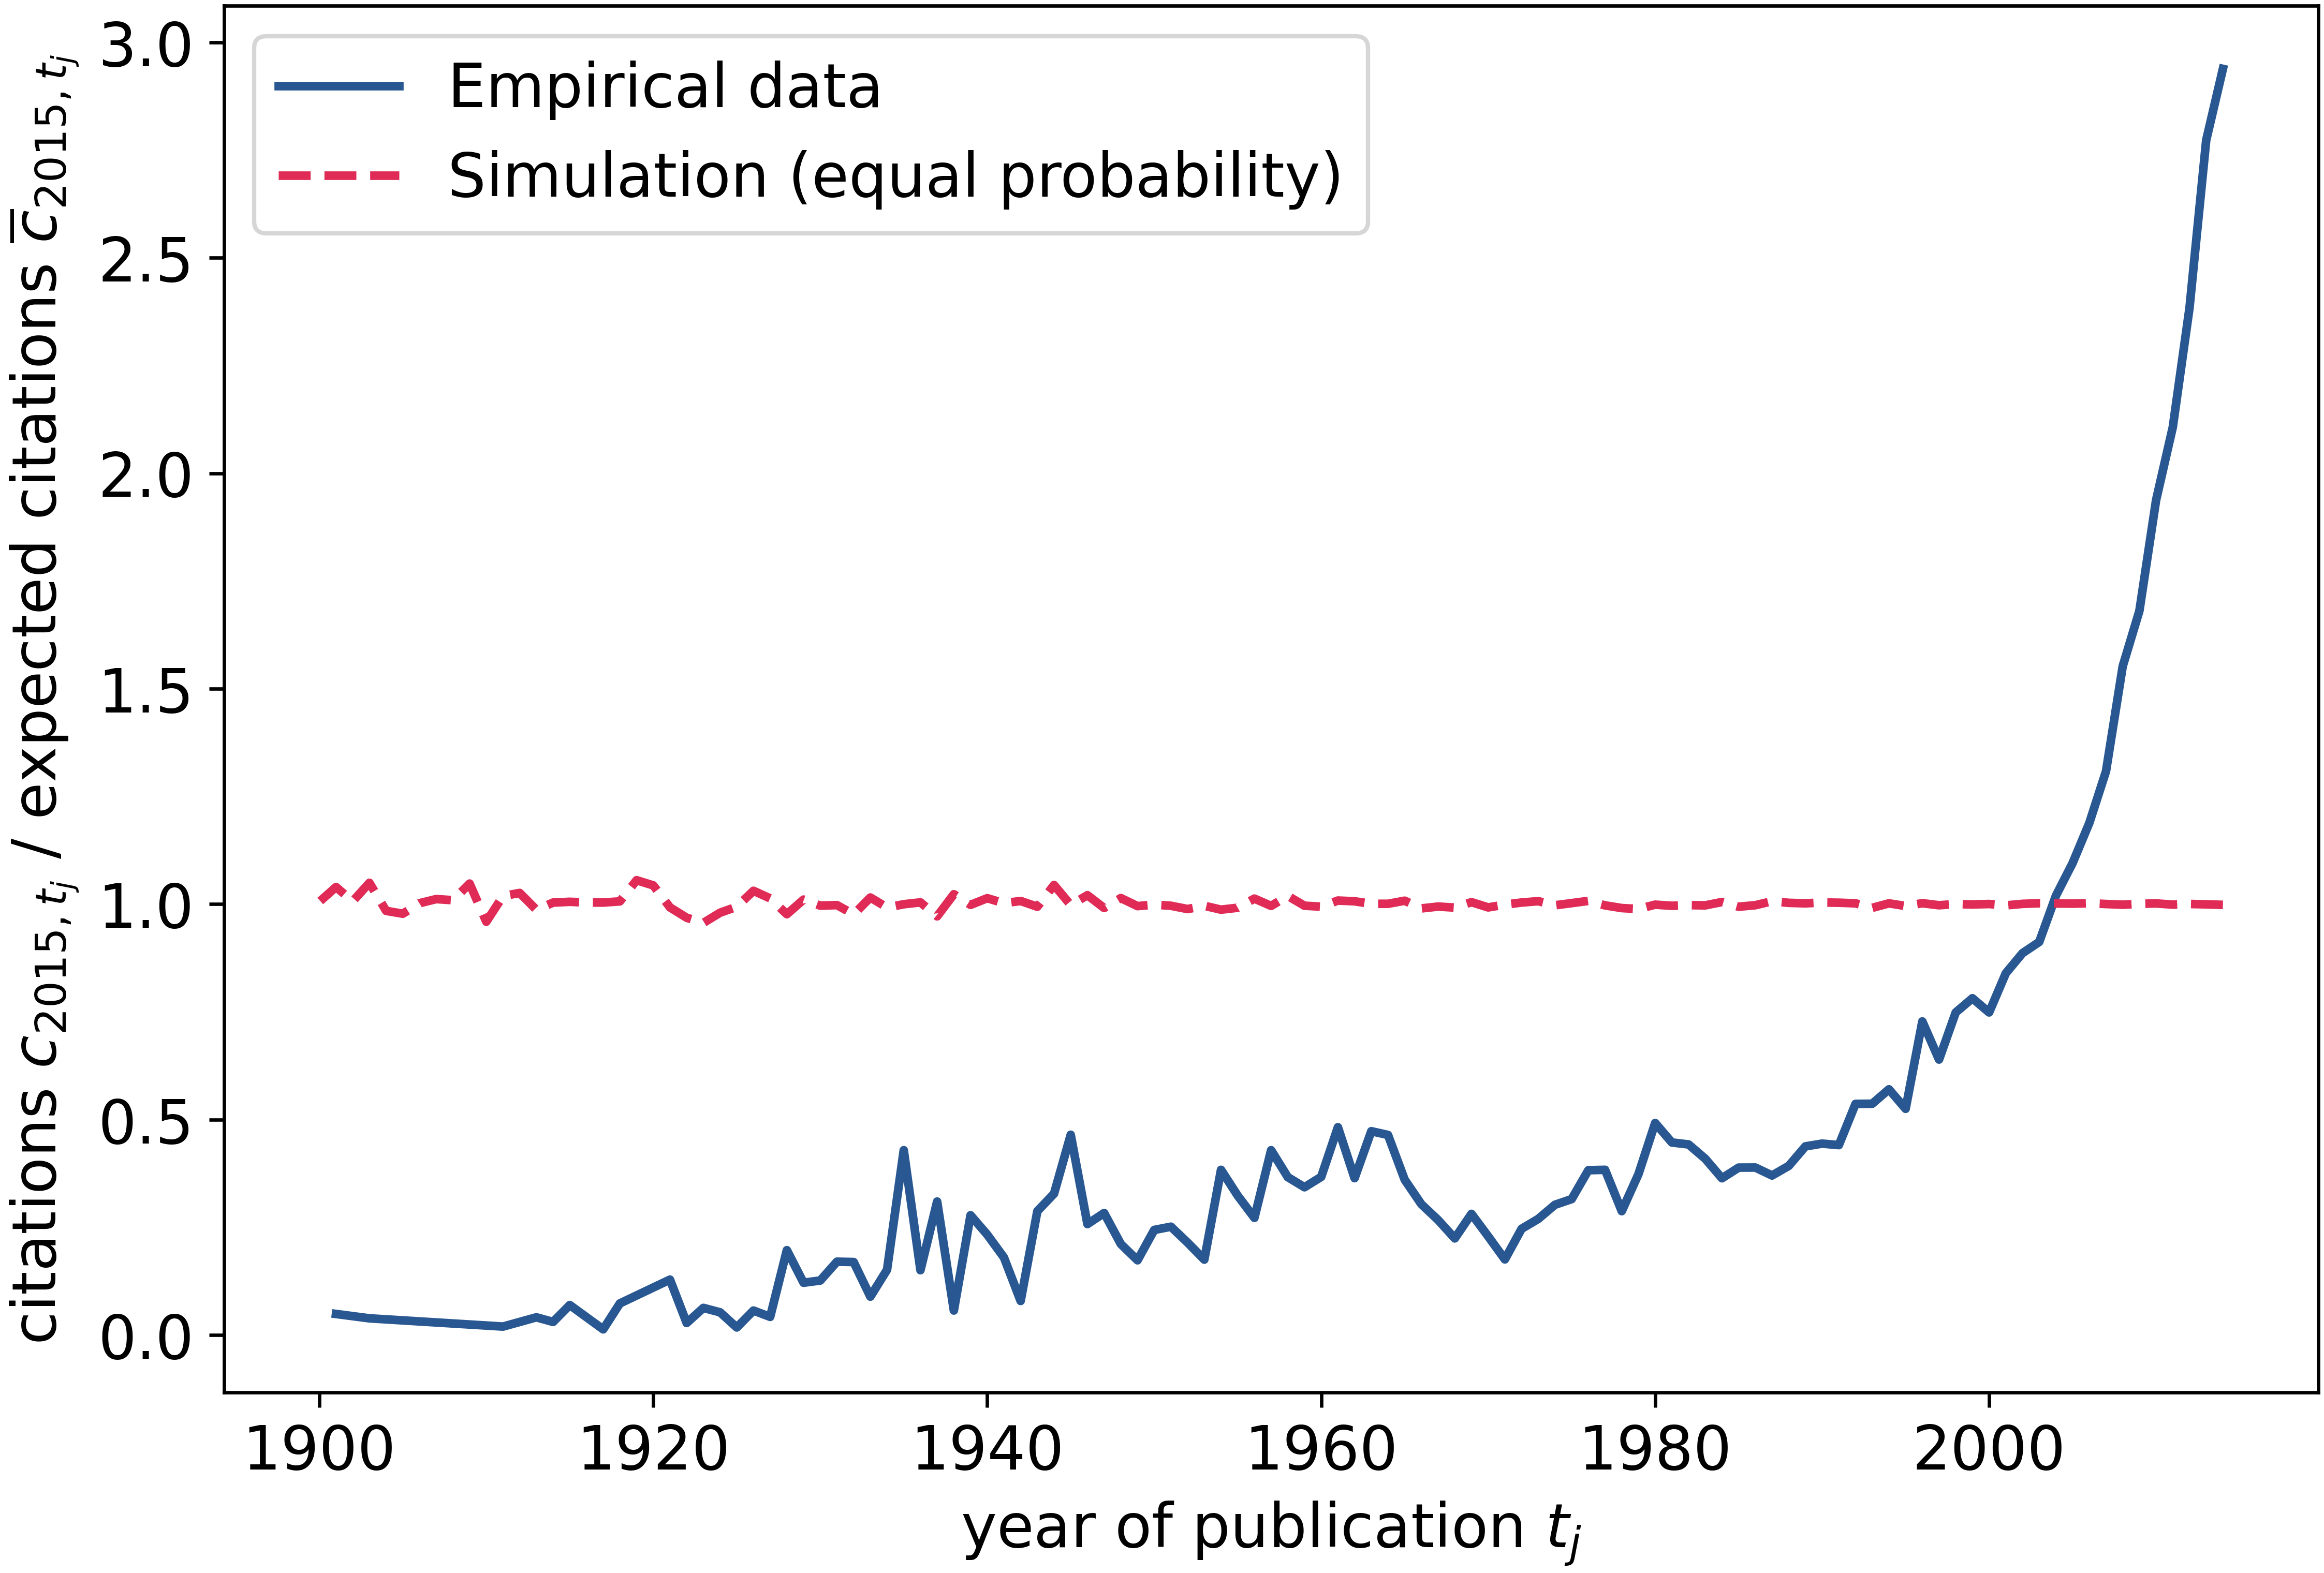
\includegraphics[width=0.7\columnwidth]{figures_aps/SI1.png}
	\caption{Forgetting curve for the APS citation network for the empirical data (blue), and the simple simulation where every paper is equally probable to get cited (red, dashed).
	}
	\label{fig:si1}
\end{figure}


\subsection{Milestone significance}
\label{SIM2}

In the forgetting curve in Fig.~\ref{fig:aor2} (b) we observed spikes coinciding with the publishing years of the top 30 papers. SI Fig.~\ref{fig:vitosplot} shows how these spikes develop over the years.

We want to show that these spikes can be caused by works of exceptional quality, here called milestones. To do so, we calculate the relative share $cit_{ms}$ of citations that go to milestone papers, compared to citations that go to all papers. The calculation is simple: For each year, we count the number of citations to milestone papers published in that year, divided by the total number of citations to all papers published in that year.

We then average this value over all the years when milestone papers were published. We find, that in the years when milestone papers were published, they attract around $6\%$ of all citations. If we repeat the analysis but consider only citations from papers published in 2015, the last year of our data set, we find that in the years when milestone papers were published, these milestones attract around $14\%$ of all citations of papers published in 2015. Since the forgetting curve is directly proportional to the number of citations, these values are indeed high enough to cause a visible spike in the forgetting curve. 


\begin{figure}[!ht]
	\centering
	 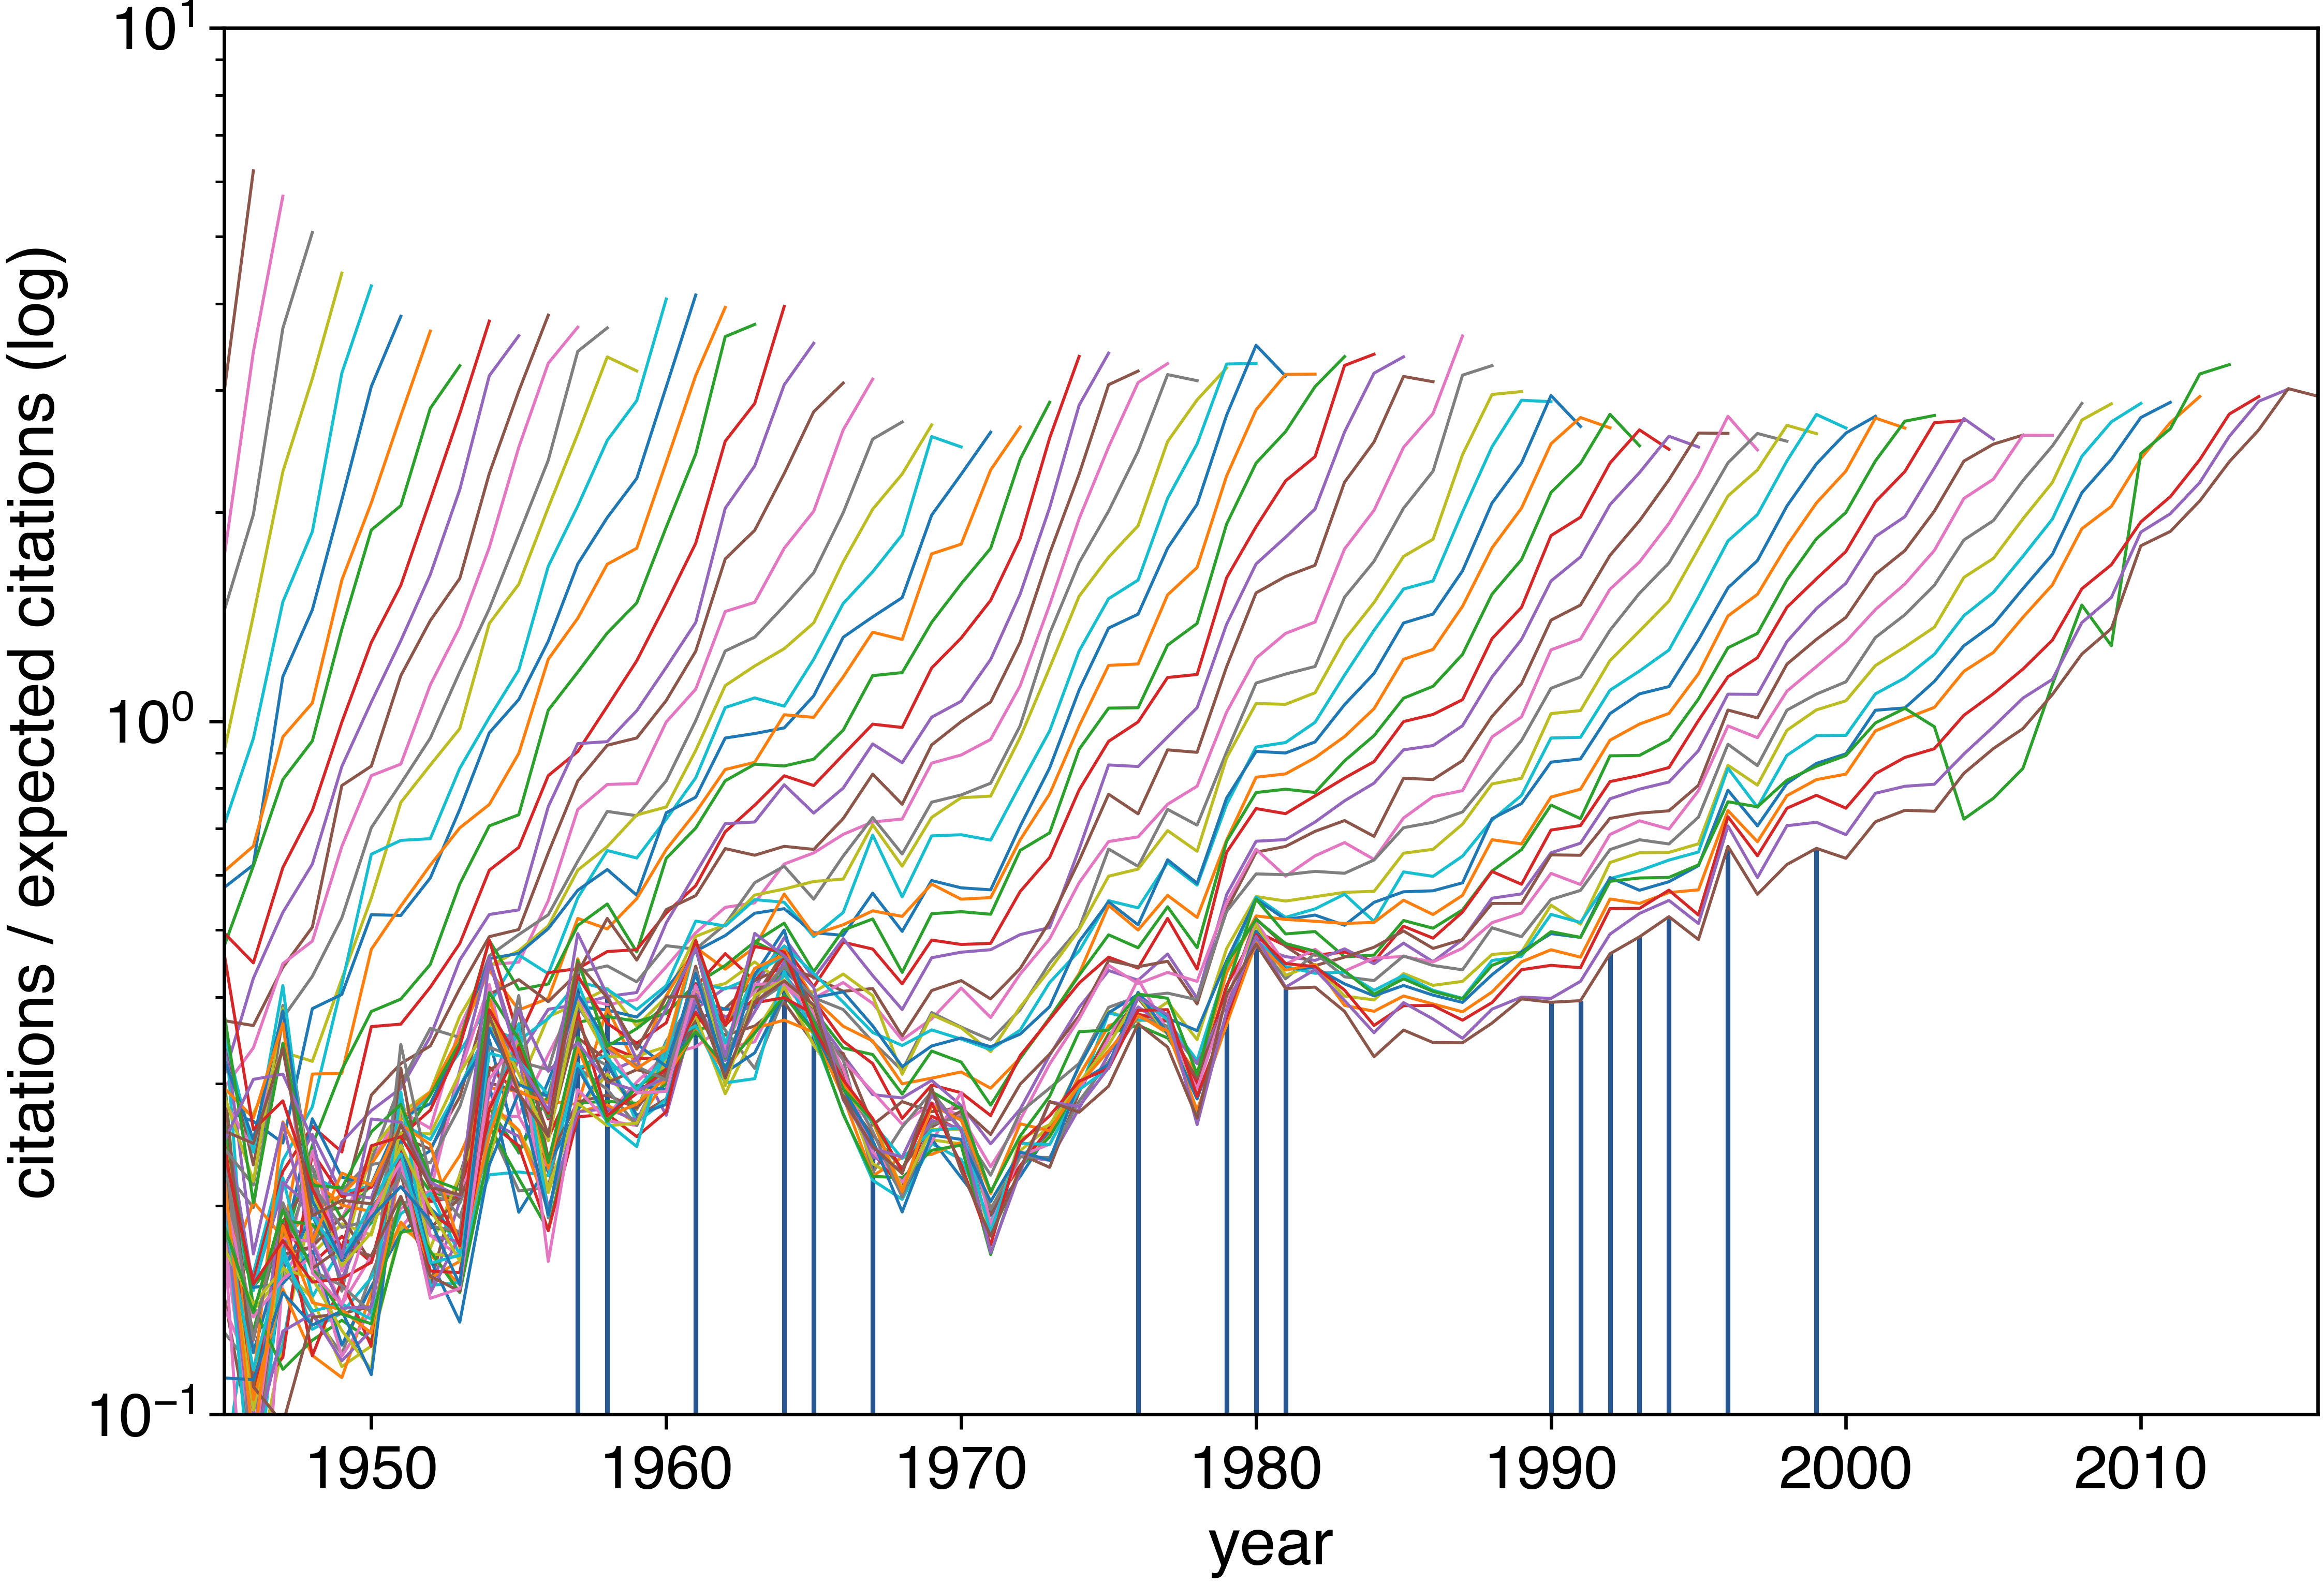
\includegraphics[width=0.7\columnwidth]{figures_aps/4.png}
	\caption{The forgetting-curves of the APS. Each line represents the forgetting-curve for papers published in the year after the right-most point of the curve (e.g. if the curve ends in 2014, it is the forgetting curve of papers published in 2015). Years where milestone papers were published are marked with vertical lines. In these years, one can observe the formation of spikes due to the adoption of the milestone paper by following the vertical line from the top (earlier years) to the bottom (recent years).
	}
	\label{fig:vitosplot}
\end{figure}



\subsection{Measuring the attachment kernel}
\label{SI3}

To measure the attachment kernel, $f(k,t)$, we modify the method originally used by Newman in co-authorship networks \cite{Newman2001} to two dimensions. We then apply it to the 120 years of empirical citation data of the American Physical Society.
In this method, we go through the papers of the APS, one by one, ordered in time, and build a histogram from which we can read off the attachment kernel. The steps included are as follows. First, we go through the APS citation network $M_{i,j}$ node by node and link by link,  starting from the first paper ever published and ending on the most recent paper. At each point in time, the probability of a paper $j$ citing a specific paper $i$ with age,  $t$, and $k$ citations, is given by:
%
\begin{equation}
    P(k,t) = f(k, t) \frac{n(t_j)}{N(t_j)} \, , 
\end{equation}
%
where $n(t_j)$ is the number of papers present at publishing time $t_j$ of paper $j$ that have the same exact values of $k$ and $t$ as paper $i$,  and $N(t_j)$ is the total number of papers present at that time. Then the attachment kernel $f(k,t)$ can be estimated from a histogram where each contribution is weighted with the inverse probability $\frac{N(t_j)}{n(t_j)}$. A sketch of this method is shown in Fig. \ref{fig_newman}.
From the resulting histogram, we can extract slices for fixed values of $k$ or $t$. These let us fit the functions in $k$ and $t$ respectively. If the slices only differ in a factor, then the kernel is of the form $f(k,t)=g(k)h(t)$. We find, that this is true in good approximation for the bulk of average publications. 

\begin{figure}[!ht]
	\centering
	 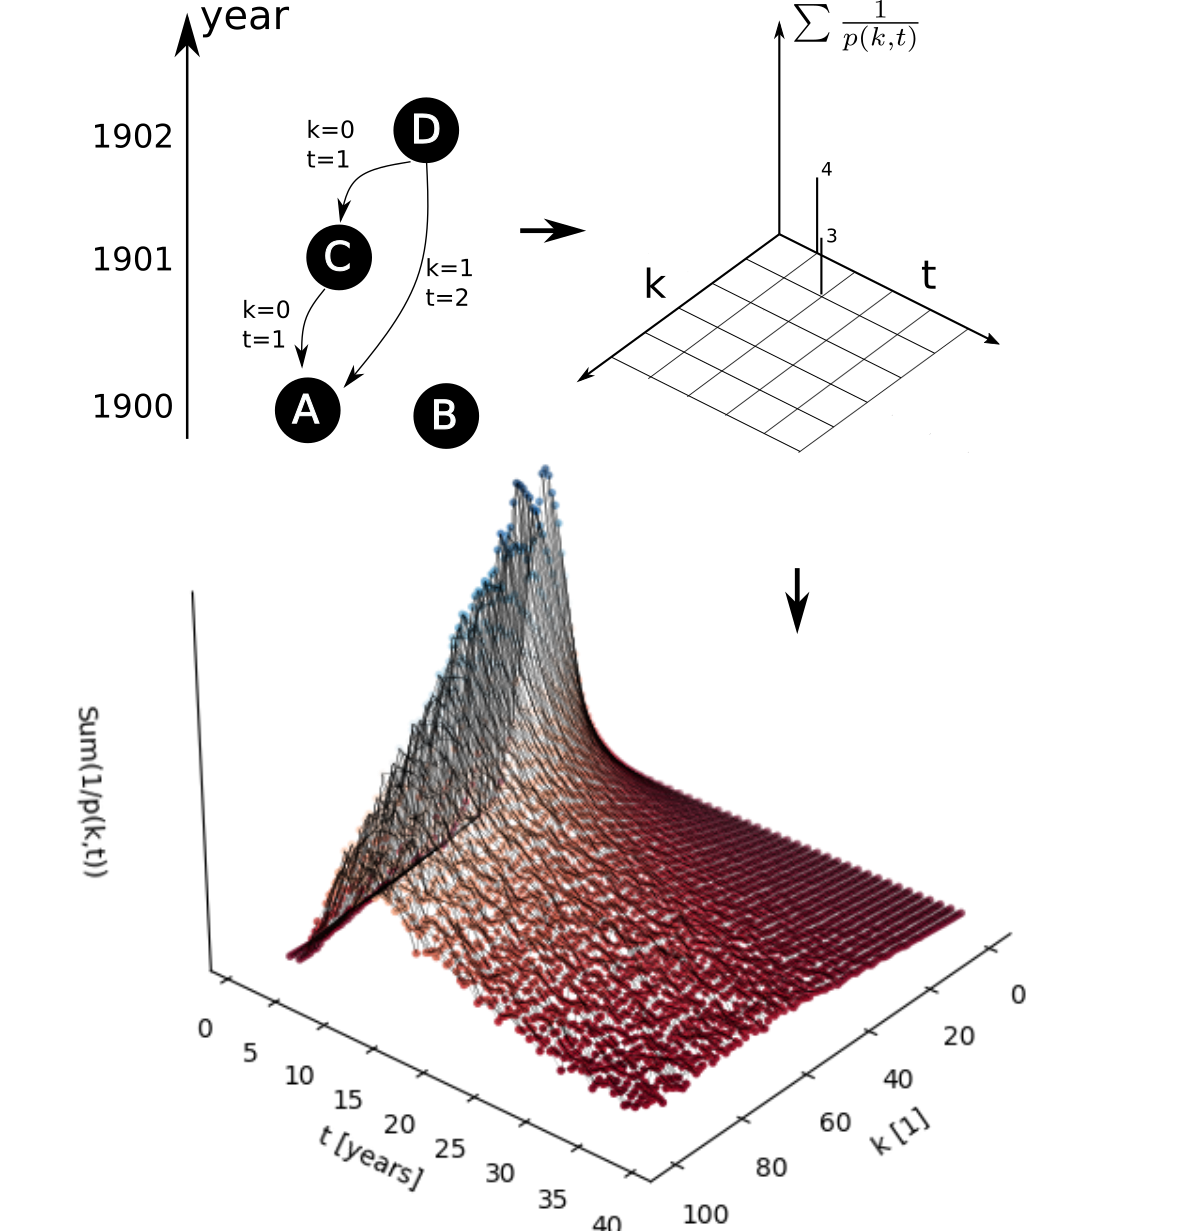
\includegraphics[width=0.8\columnwidth]{figures_aps/newman.png}
	\caption{Approximating the kernel $f(k, t)$ of the APS citation network.\\
	a) The citation network is rebuilt paper by paper. Each black dot is a paper, each link is a citation. The papers are published in alphabetical order. For reach citation, the values of k, t and the state of the network are used to build the histogram.\\
	b) The histogram is generated as the sum of the inverse probabilities when reconstructing the citation network. \\
	c) The histogram for the entire network. This landscape in k and t represents the shape of the probability kernel $f(k, t)$. The shape is only representative for areas where sufficient data is available.
	}
	\label{fig_newman}
\end{figure}

The result is a two-dimensional histogram that approximates the probability kernel, $f(k, t)$. Note, however, that many combinations of $(k, t)$ are underrepresented in the history of the APS and thus also in the histogram. For example, it is evident that there are very few papers that have a high number of citations already in the first few years. Thus, the histogram is only representative in areas where sufficient data is available. For this reason, it is not practicable to directly fit a function to the histogram.

By fixing $k$ or $t$ to specific values, slices in $t$ or $k$ can be extracted from the surface. We slice the landscape for all integer values of $k$ and $t$ and fit functions to the slices. If the probability kernel is factorizable, $f(k, t)=g(k)h(t)$, then the slices would only differ by a factor. We fit a linear function $g(k) = k$ and a power $h(t) = t^{-\alpha}$. From this, we calculate an average exponent as the weighted average over all exponents, where the weights correspond to the number of times a particular value of $k$ was observed in the history of the APS.

\subsection{Milestone attachment kernel}
\label{SIM4}

In the introduction, we discussed that some old publications receive exceptionally high numbers of citations. We call these the milestone papers. In the context of a citation network, we define them through their citations and take the top 30 most cited papers of all time that are not review papers. The choice is arbitrary, but the results hold for different values as long as the papers are receiving numerous citations. 

The milestone papers are exceptions, they stand out from the bulk. As such, their number is low, and the statistics are not sufficient to measure their attachment kernel with the method described in~\hyperref[SI3]{SI 3}. Instead, we propose a slightly different method, described below. 

To figure out an estimator for the probability of being cited, we draw a comparison to an urn model. Suppose we have an urn with different colors of balls. We are only interested in one special color. There are multiple copies of that color in the urn. In each run, we draw with replacement until we draw a ball of our color. If we do many runs, and on average it takes $n$ draws until a ball of our color is drawn, then the most plausible estimator for the probability of drawing our color would be $\frac{1}{n}$.

In addition to that, we introduce the concept of intrinsic time for a citation network. Each citation event, where any paper is cited, represents one discrete time step in intrinsic time. For a milestone paper m, the probability of being cited at any intrinsic time step $\tau$ is given by:
%
\begin{equation}
    p_m = \frac{f(k_{m, \tau}, t_m, \alpha_m)}{\sum_i f(k_{i, \tau}, t_i, \alpha_i)} \, ,
\end{equation}
%
where f is the probability kernel of the form:
%
\begin{equation}
    f_i = f(k_{i, \tau}, t_i, \alpha_i) = (k_{i, \tau}+1)(t_i + 1)^{-\alpha_i} \, , 
\end{equation}
%
and $k_{i, \tau}$ is the in-degree of paper $i$ at intrinsic time-step $\tau$, $t_i$ is the age of paper $i$ in years and $\alpha_i$ is the forgetting-exponent of paper $i$.\\
The most likely estimator for the number of citations $C$ it takes until paper m is cited is $\frac{1}{p_m}$. We can estimate:
%
\begin{equation}
    C \approx \frac{1}{p_m} = \frac{\sum_i f_{i, \tau}}{(k_{m, \tau}+1)(t_m + 1)^{-\alpha_m}}
\end{equation}
%
leading to 
%
\begin{equation}
\label{eq_alpha}
    \alpha_m \approx \log(\frac{C (k_{m, \tau}+1)}{\sum_i f_{i, \tau}}) \frac{1}{\log(t_{m, \tau}+1)} \, .
\end{equation}
%
We know $k_{m, \tau}$ and  $t_{m}$. $C$ is the number of citation events between two events where the milestone paper $m$ is cited. 
The $\alpha_i$ are unknown, but they only appear in the sum. Since we have a good approximation for them, supposedly, the sum should be approximated correctly. Thus, we can estimate $\alpha_m$ directly. For each time the milestone paper $m$ is cited, we get a different $C$ and $k_{m, \tau}$ is increased by 1, so we collect a set of values for $\alpha_m$
%
\begin{equation}
\label{eq:msalpha}
    \overline{\alpha}_m = \log(\frac{C(k_m+1)}{\sum_i f_{i, \tau}})\frac{1}{\log(t_{m, \tau}+1)} \, . 
\end{equation}
%
These values can be averaged (before applying the logarithm) in order to determine an average exponent. However, if we apply a linear fit to the set of values for $\alpha$, we notice a general slightly increasing trend. This suggests that in our approximation for the kernel, $f(k,t) = (k+1)(t + 1)^{-\alpha}$, the functions of $k$ and $t$ cannot be separated completely for milestone papers. Instead, there is a small dependency on $k$ in $\alpha$. A more fitting approximation for milestone papers is thus given by $f(k,t) = (k+1)(t + 1)^{-(a+bk)}$ i.e., the exponent $\alpha$ is a linear function of $k$ with a very small and positive slope.

To validate the method, we construct the null model explained in~\hyperref[SI5]{SI 5}. We simulate the full system and then repeat the measurement of the exponent in the simulated system. Since the exponent in the attachment kernel of the simulation are configuration parameters, we have perfect knowledge of them. Thus, we can compare the values we measure with the ones we used as an input. If the measurement method is valid, we would expect these values to be the same, apart from some noise. Indeed, we measure an average absolute deviation of $\Delta\alpha=0.1$. If binning is used to reduce the noise, the average absolute deviation can be reduced to $\Delta\alpha=0.01$. The result for one example paper is shown in fig. \ref{fig_mspexp}.

\begin{figure}[!ht]
	\centering
	 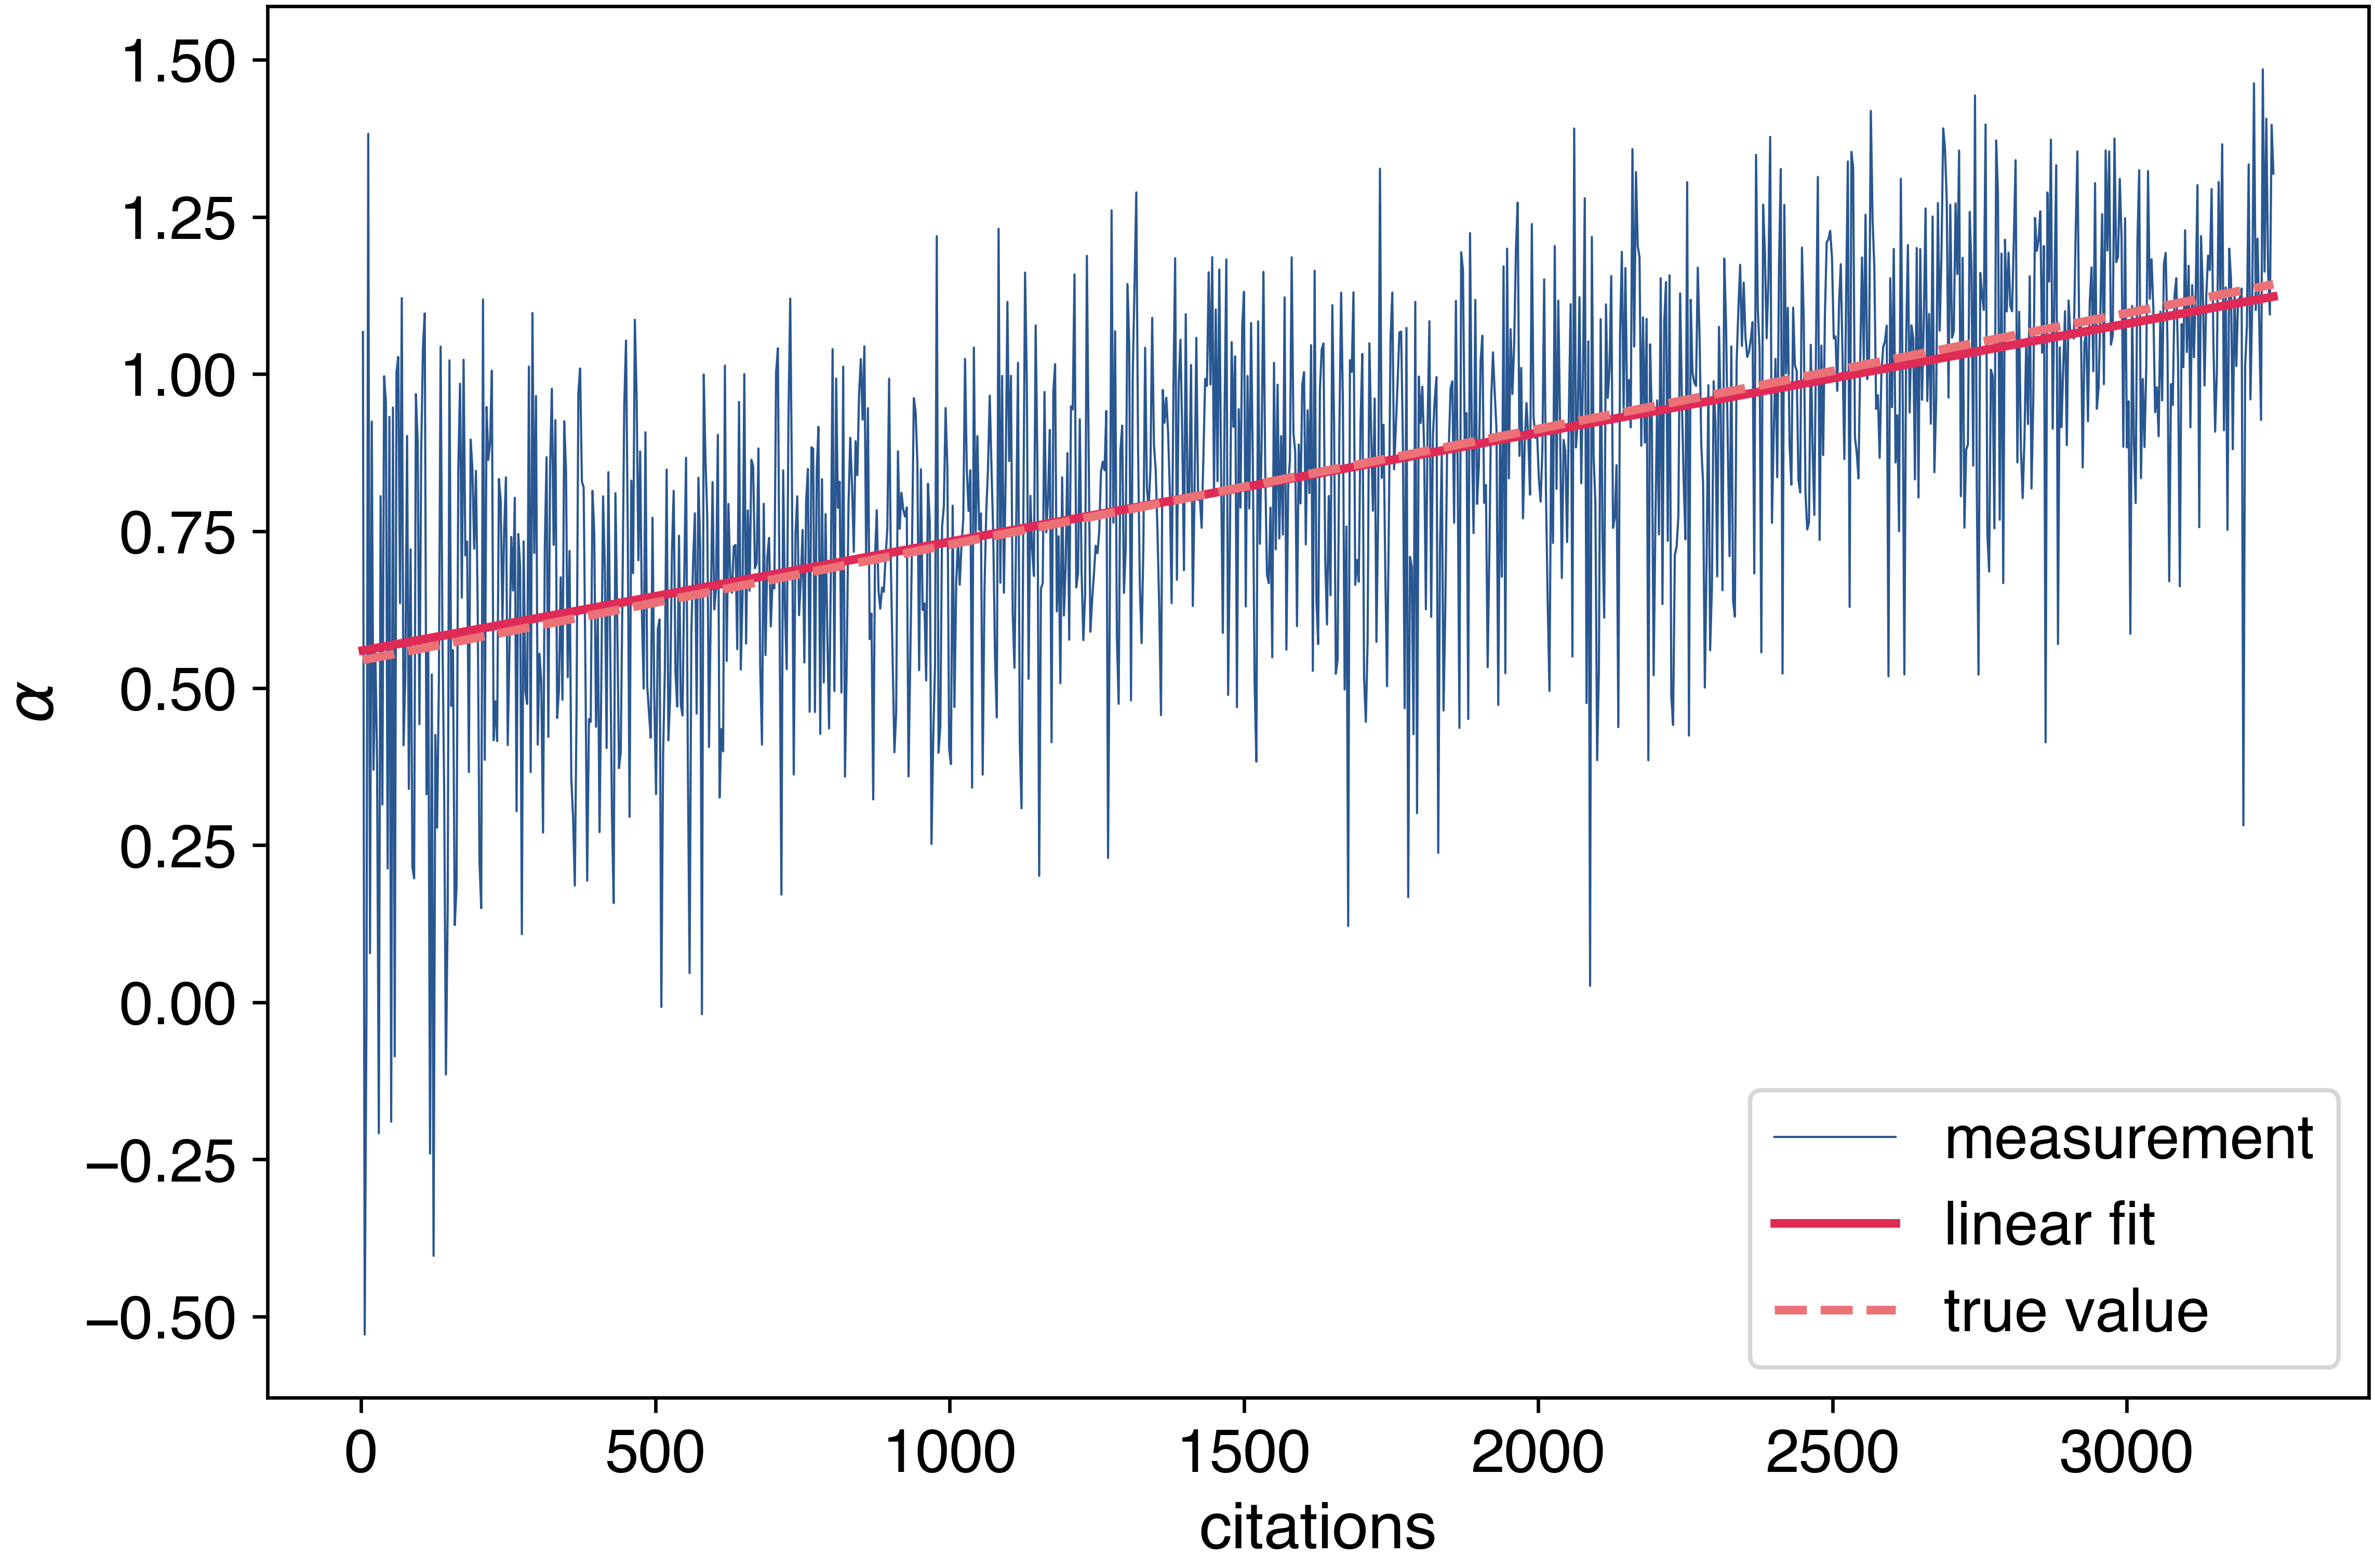
\includegraphics[width=0.7\columnwidth]{figures_aps/7.png}
	\caption{Exponent $\alpha$ of $(k+1)(t + 1)^{-\alpha}$ vs in-degree k for a representative milestone paper, measured on the simulated null model. Blue: individual measurements of $\alpha$, Red: linear fit on the individual measurements, Orange, dashed: true value (simulation input)
	}
	\label{fig_mspexp}
\end{figure}

Two additional effects might have an impact on the measured value and thus need to be ruled out. First, in equation \ref{eq:msalpha} the sum $\sum_i f_{i,\tau}$ changes after each citation event (each intrinsic time step $\tau$). For the calculation, we take the value at the end of the interval, i.e., the value of $\tau$ at the time when the milestone is cited. This is technically inaccurate, but the inaccuracy is very small. We measure this both at the beginning and the end of the interval, confirming that the sum changes only by an insignificant amount. Thus, this effect can be neglected.
Second, each paper cites n other papers, but each of the cited papers can only appear once in the reference list. Thus, the probabilities for getting cited by one paper change depending on what else was cited by the same paper. Also, this effect can be neglected since on average the number of references per paper is very small compared to the total number of citable papers. 

\subsection{Null model}
\label{SI5}

We construct a null-model of the APS citation dynamics. In this model, we keep all publishing dates and out-degrees (number of references) of real papers from the empirical data, but we attach each outgoing link to a random paper that was published before based on the probability kernel $f(k,t)$. For milestone papers we use the exponent that we determined from the real data, for the bulk of average papers we take the average exponent. A sketch of the null-model is shown in  SI Fig. \ref{fig:null}.

\begin{figure}[!ht]
	\centering
	 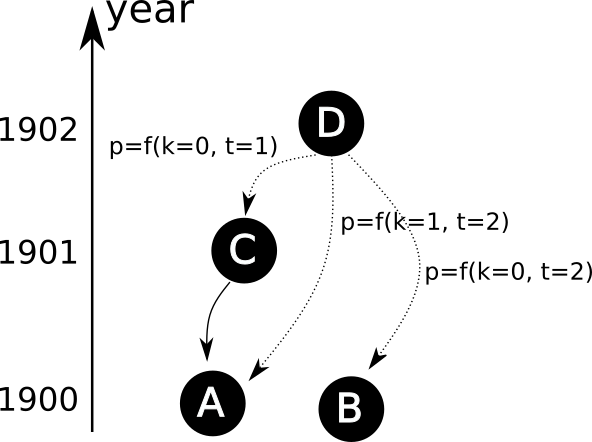
\includegraphics[width=0.6\columnwidth]{figures_aps/null.png}
	\caption{Null model of the APS citation dynamics. Papers are published in the same order, at the same time and with the same out-degree (number of references) as the papers of the APS citation network. Each paper randomly cites papers that were published before with a probability proportional to the probability kernel, $f(k,t)$.
	}
	\label{fig:null}
\end{figure}


\subsection{Milestone simulation performance}
\label{SI6}

Figure \ref{fig:SI6} shows a comparison of forgetting curves and allows the estimation of the simulation's performance in terms of milestones. Three forgetting curves are plotted there. The first (blue, solid) is the forgetting curve of the empirical APS. The second curve (red, dashed) is the forgetting curve of the empirical APS, with all reference to milestones removed. By comparing the first two curves, one can understand how milestones affect the entire forgetting curve. The third curve represents our null-model simulation. One can see, that in almost all cases where there is a difference between the curves with and without milestones, the simulated curve has a spike of comparable magnitude.

There is one apparent exception in the year 1935, that is not captured well in the simulation. It concerns the famous paper titled "Can Quantum-Mechanical Description of Physical Reality Be Considered Complete?" by Einstein, Podolsky and Rosen. Curiously, this paper received less than 10 citations from papers published in the APS in the first 15 years after being published, presumably in part due to the war. It wasn't until the 1990s that this paper gained traction and began to be widely quoted. As a result, it is known as a prime example of a "sleeping beauty." This late discovery and peculiar citation pattern are not adequately reflected by a time-independent forgetting exponent, and as a result, the citations of this publication are underestimated in the simulation.

\begin{figure}[!ht]
	\centering
	 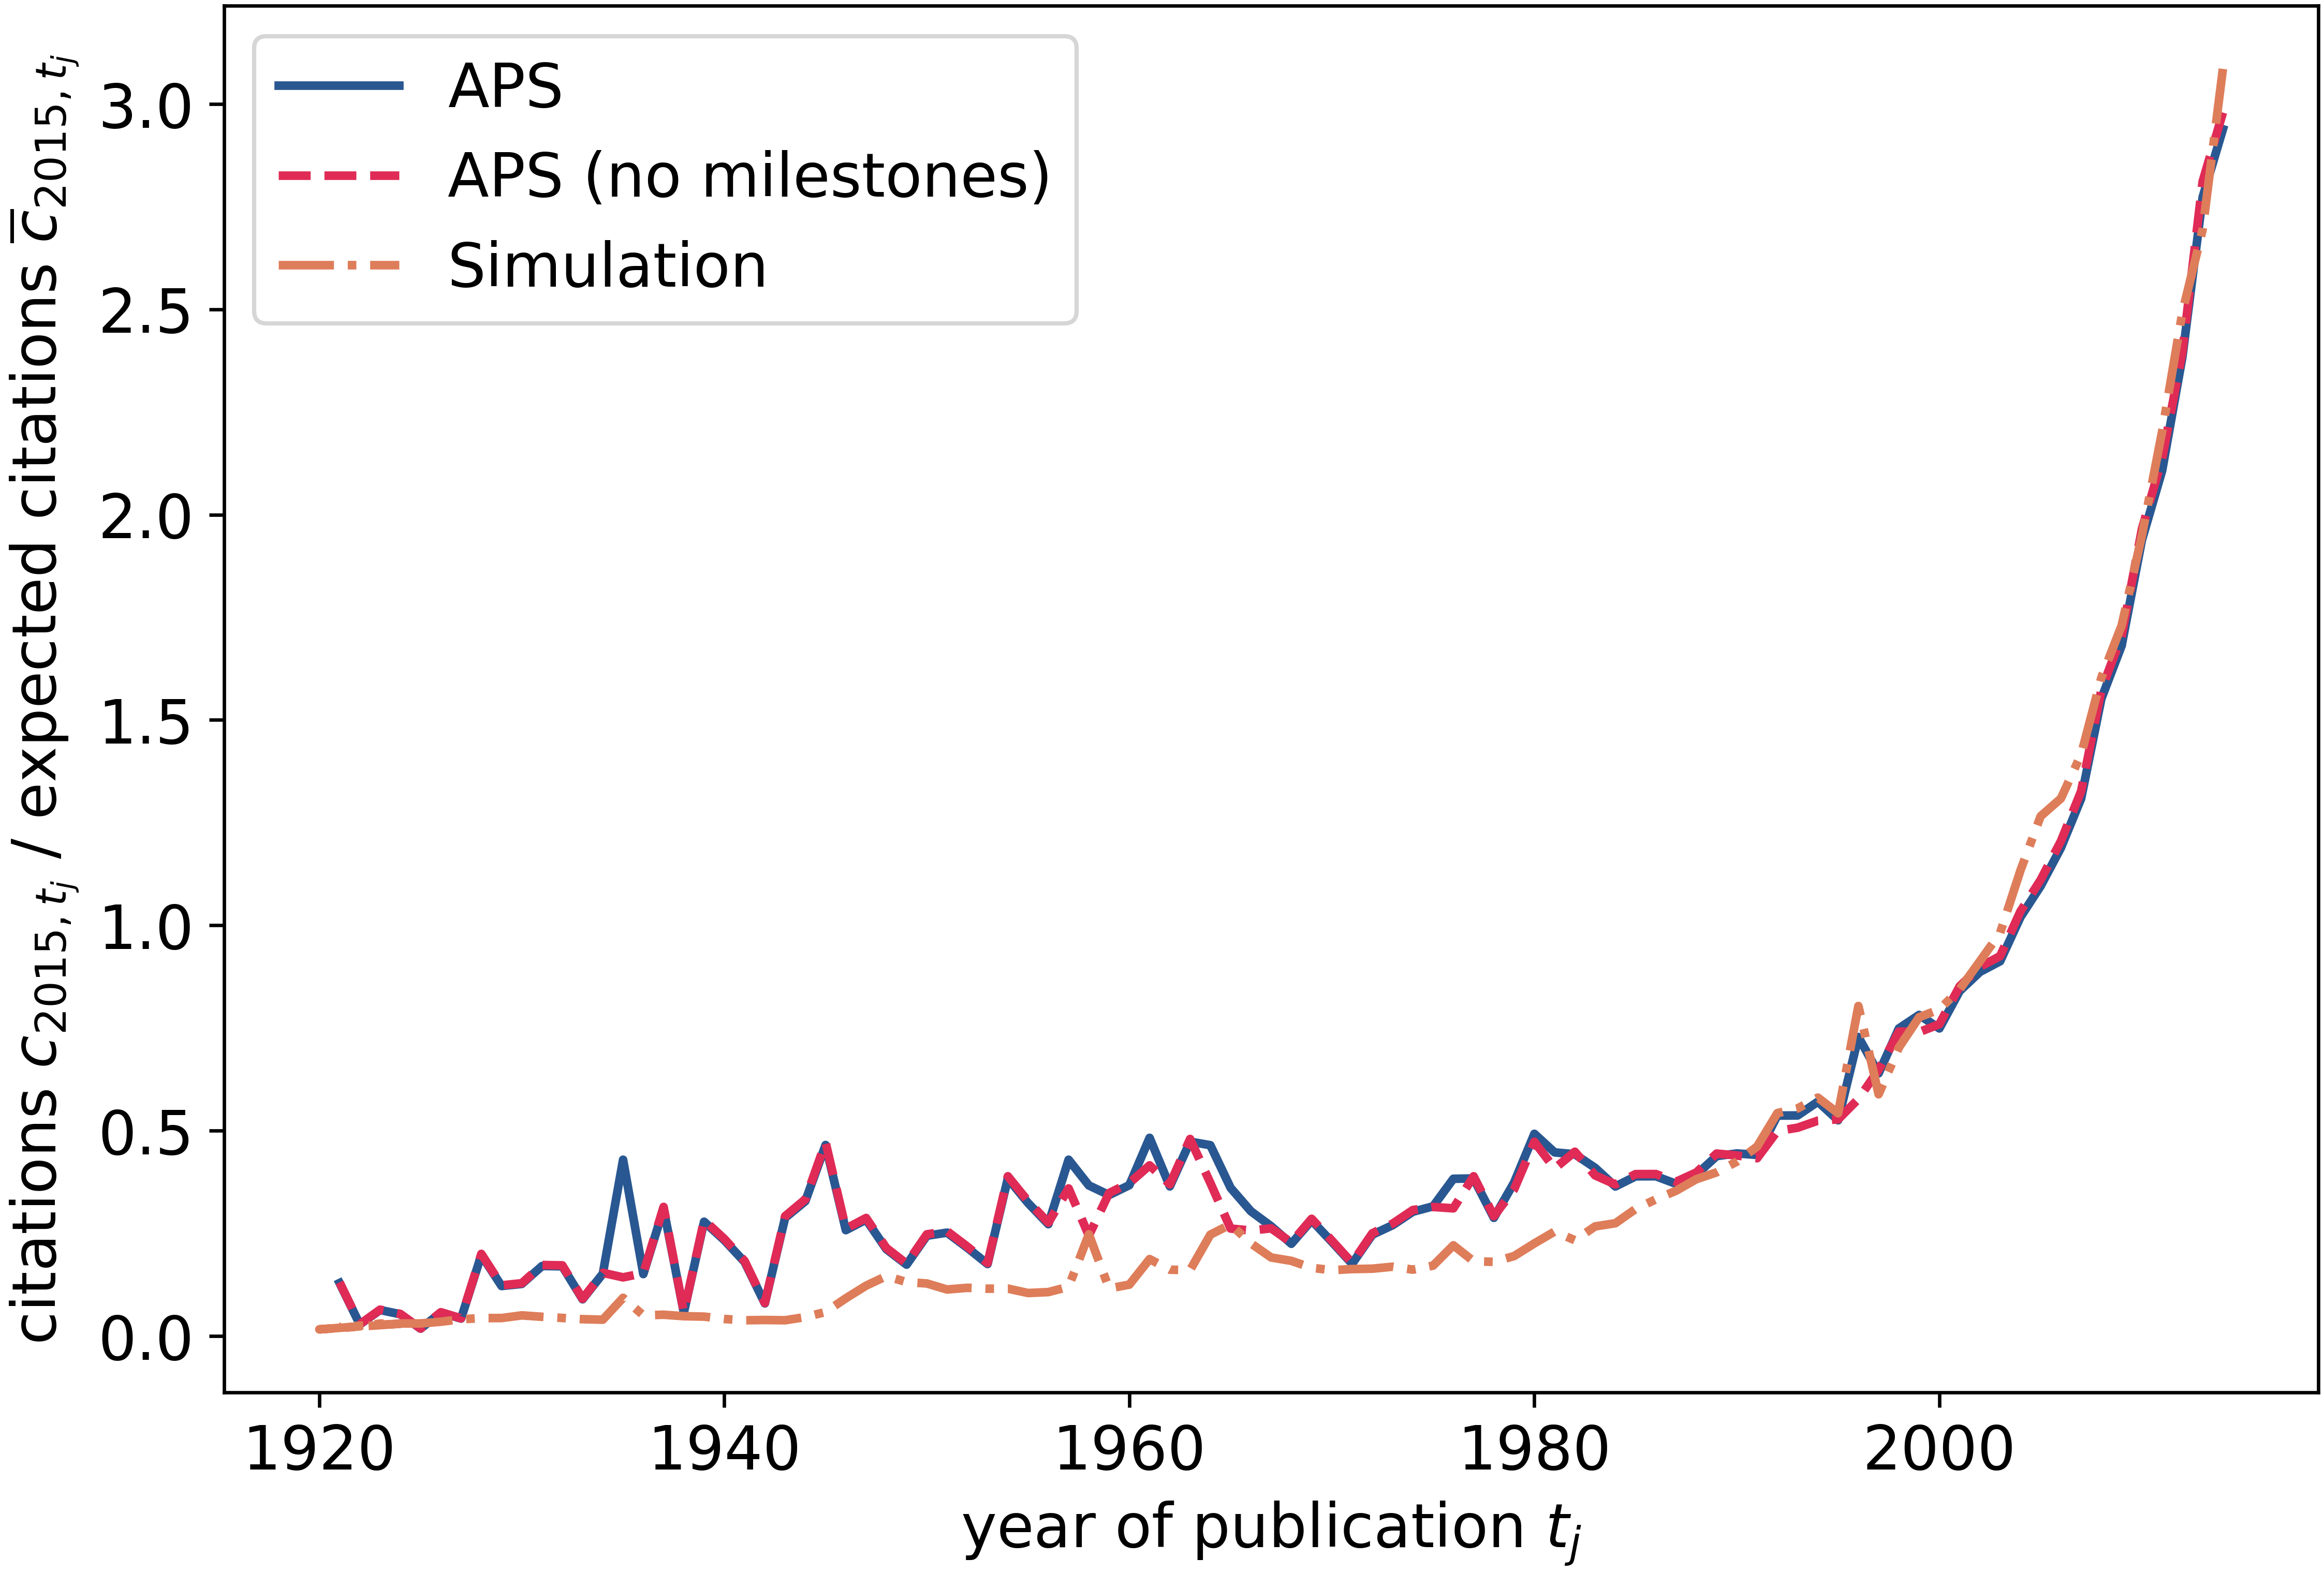
\includegraphics[width=0.7\columnwidth]{figures_aps/SI7.png}
	\caption{A comparison between forgetting curves. Forgetting curve of the empirical APS (blue, solid), forgetting curve of the empirical APS where citations to milestones were removed (red, dashed) and null-model simulation (orange, dashed and dotted). The apparent outlier in 1935 is the famous paper by Einstein, Podolsky, Rosen, and a prime example of a "sleeping beauty". 
	}
	\label{fig:SI6}
\end{figure}


\subsection{Citation trends}
\label{SI7}
To reveal general citation trends in the APS, we investigate the average number of citations that a paper published in a certain year receives, see fig. \ref{fig_SI_cit}. Note that the steep decline during the last decade is due to the papers not having had enough time to accumulate all their citations yet.

\begin{figure}[!ht]
	\centering
	 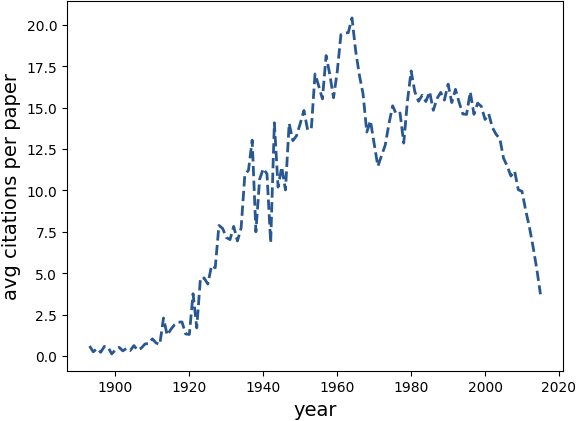
\includegraphics[width=0.7\columnwidth]{figures_aps/8.png}
	\caption{
	Average number of citations that papers published in each year between 1893 and 2015 received. Note that the steep decline during the last decade is due to the papers not having had enough time to accumulate all their citations yet.
	}
	\label{fig_SI_cit}
\end{figure}

To show that an increasing number of citations go to milestone papers, we plot the fraction of references of all papers published in a certain year, that reference highly cited papers (papers with $\geq 1000$ citations) over the total number of references. This is shown in fig. \ref{fig_SI_ms1}.  

\begin{figure}[!ht]
	\centering
	 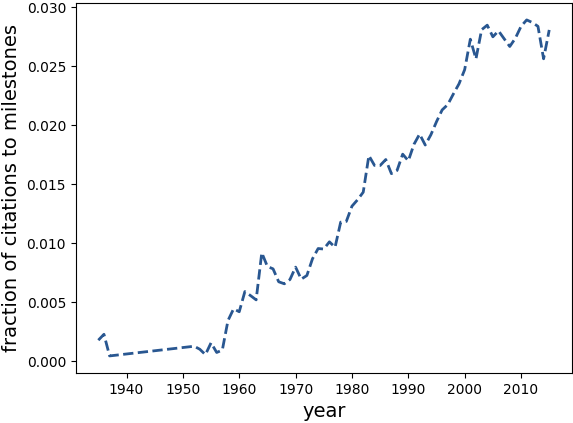
\includegraphics[width=0.7\columnwidth]{figures_aps/9.png}
	\caption{
	    Fraction of references to highly cited papers ($\geq 1000$ citations) over references to all papers for each year between 1893 and 2015.
	}
	\label{fig_SI_ms1}
\end{figure}

In fig. \ref{fig_SI_ms2} we show the number of highly cited papers (papers with $\geq 1000$ citations) published in a certain year over the total number of papers published in that year.

\begin{figure}[!ht]
	\centering
	 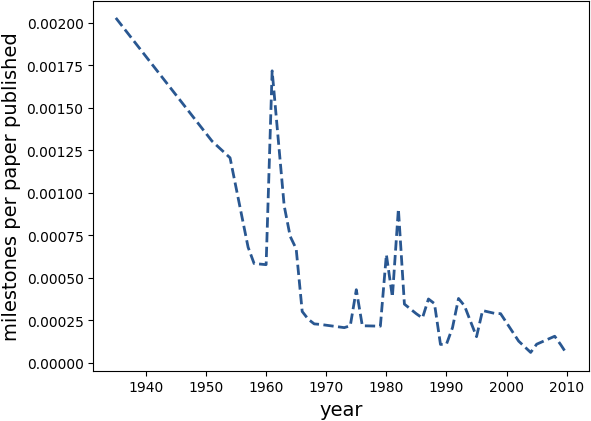
\includegraphics[width=0.7\columnwidth]{figures_aps/10.png}
	\caption{
	Fraction of highly cited papers published ($\geq 1000$ citations) over total number of papers published for each year between 1893 and 2015.
	}
	\label{fig_SI_ms2}
\end{figure}



% ========================= CHAPTERS ======================================	
\chapter{Inbreeding: Academic self-hires and internationalization}

There is an increasing need to account for how institutions internationalize \cite{hoekman2009geography, robinson2019many}. Evidence suggests that cross-national mobility flows are increasing \cite{sugimoto2017scientists} as is the strengthening of global collaborative research networks \cite{wagner2017open}. Research institutions foster internationalization as they compete to attract and retain foreign talent in a global market \cite{hazelkorn2015rankings}, with foreign-born researchers accounting for 43 per cent of life sciences postdoctoral research in Europe and 56 per cent of these coming from outside the European Union \cite{moguerou2008}. As a result, there is a policy interest in monitoring and understanding the process of academic mobility and internationalization of universities \cite{jacob2013scientific, sugimoto2017scientists}.

The lack of global and harmonized datasets has been a persistent challenge in developing global indicators of mobility \cite{welch2018}. This is especially problematic at the institutional level, which besides functioning author-disambiguation mechanism requires clear institutional identification \cite{donner2020comparing}. Recently, bibliometric databases have significantly improved the consistency of publication metadata, particularly author--affiliation linkages, allowing to track affiliations of individual researchers and opening up new opportunities for studying long-term mobility patterns at scale \cite{moed05, sugimoto2016}. Previous work has been concerned exclusively with the quantification of the movement of scholars across countries and disciplines \cite{robinson2019many}. However, evidence on institutional mobility has been lacking.

In this chapter, we aim to help in closing this gap by delivering novel insights on the composition of the academic workforce of universities and national research systems worldwide. We base our results on the Dimensions database and the Global Research Identifier Database (GRID). We propose three indicators by which institutional workforces can be characterized based on researchers' first and most recent institution of affiliation. By comparing the institution to which researchers were affiliated in their first publications with their most recent one, we distinguish between: 

\begin{itemize}
    \item Insiders, defined as researchers who are currently affiliated to the same institution to which they were affiliated in their first publications; 
    \item Domestic outsiders, that is, those who were originally affiliated to a different institution within the same country from their current one; and
    \item Foreign outsiders, researchers who were originally affiliated
to an institution located in a different country
from their current one.
\end{itemize}

\subsection{Academic mobility, internationalization, and institutional inbreeding: implications for scientific enterprise and research careers}



In recent years, bibliometric databases have substantially improved the consistency and quality of the metadata extracted from publications, particularly the author-affiliations linkages from scientific publications. Furthermore, author-name disambiguation algorithms have been implemented for most large bibliometric databases, such as Web of Science, Scopus, and Dimensions. Most of these algorithms benefit from open systems for the unique identification of scholars like ORCID. These developments have led to new scientometric approaches to track aggregated mobility patterns between countries and regions.

However, when it comes to the mobility of researchers between institutions, evidence is scarce due to the lack of harmonized affiliation data at the micro level. This situation is changing due to the implementation of advanced approaches for affiliation harmonization like the approach used for the Leiden Ranking, or, more recently, the Global Research Identifier Database (GRID), that currently covers more than 98,000 research institutions worldwide. The availability of these harmonized registries enables the identification of affiliation changes in the careers of scholars. In this blog post, we illustrate how author-affiliation information can be used to develop mobility indicators at the institutional level and explore the many possibilities this offers for the study of scientific mobility.

We propose institutional mobility indicators based on researchers’ mobility flows in 22 major fields of science across 1,130 Leiden Ranking institutions from 64 countries. We base our indicators on data from the Dimensions database and Global Research Identifier Database. We use researchers’ first and last affiliations to estimate the extent authors have moved across institutions as well as countries. For each institution, we quantify the shares of researchers with the same affiliation (insiders), those who came from another institution within the country (domestic outsiders), and those coming from a different country (foreign outsiders). Institutions in Central, Eastern, and Southern Europe have the highest share of insiders, whereas institutions in Northern America and Western and Northern Europe have a higher share of foreign outsiders. Foreign outsiders are most common in small and wealthy countries. No disciplinary differences are observed, as captured by the field classification scheme of Dimensions.


\section{Measuring the institutional mobility of scholars}

\section{Results}

\section{Discussion}


% ========================= CHAPTERS ======================================	
\chapter{Alignment: Scientific mobility, prestige and skill alignment in academic institutions}
Scientific discovery requires the capacity to seek, nurture, and combine internal and external sources of knowledge. Universities, in particular, serve as vital ``containers'' for the advancement and integration of this knowledge. However, because of the ``tacit'' nature of knowledge \cite{gertler2003tacit}, knowledge synergies do not emerge automatically. They rely on transfer mechanisms such as collaboration, networks, and labor mobility~\cite{cohen1990absorptive, zucker1994intellectual, gertler2003tacit, winter1982evolutionary}. Academic mobility is a particularly important mechanism for knowledge to flow effectively across people, organizations, locations, and time \cite{cohen1990absorptive, stephan2001exceptional, ganguli2015immigration}. 

Scientists are  moving between different institutions with increasing frequency \cite{sugimoto2017scientists}. According to some estimates, in 1990, about 2\% of scientists worked outside their country of origin \cite{stephan2001exceptional}. By 2000, this proportion increased to 14\% \cite{stephan2001exceptional}, and by 2015, it was estimated that about one-third of scientists were working outside their country of origin \cite{national2015revisiting}. A similar trend has been observed in Europe, where it has been reported that 7\% of hired researchers were from abroad~\cite{schiermeier2011career}. However, the presence of mobile researchers varies considerably by region and institution~\cite{machavcek2022researchers,schiermeier2011career, sugimoto2017scientists}. At Cambridge University, for example, it has been reported that more than 40\% of the faculty were foreign-born~\cite{schiermeier2011career}.  

The attraction of mobile individuals to institutions has been studied for many decades \cite{grant1996toward,stephan2001exceptional, ganguli2015immigration}, and several analyses have shown that external talent is essential for innovation \cite{cohen1990absorptive, stephan2001exceptional, stephan2012economics, sugimoto2017scientists, ganguli2015immigration}. Attracting individuals trained in various research contexts is critical for frontier research \cite{ganguli2015immigration,stephan2001exceptional, sugimoto2017scientists, lepori2015competition, franzoni2014mover, milojevic2018changing, jaffe1996flows}, as it enables institutions to explore new areas of knowledge. However, it is also a challenge faced by most research institutions worldwide \cite{lepori2015competition}. The exchange of talent  is increasingly concentrated in a handful of universities~\cite{stephan2012economics}. In the United States, for example, the most prestigious institutions attracted and trained most of the available faculty before sending them to other mid- and upper-level institutions \cite{clauset2015systematic,deville2014career}. Education systems also differ dramatically, with more prominent, well-funded universities offering more facilities, funding opportunities, and research diversity than smaller, specialized universities \cite{lepori2015competition,alvarez2021funding,costas2012approaching,lariviere2015team}. This unequal access to knowledge has significant implications for knowledge sharing across academic institutions and, more importantly, within the organization \cite{horn2007ranking,horta2009global}.

% FIGURE 1 %
\begin{figure} [!t] %[Illustrating the method]
\centering
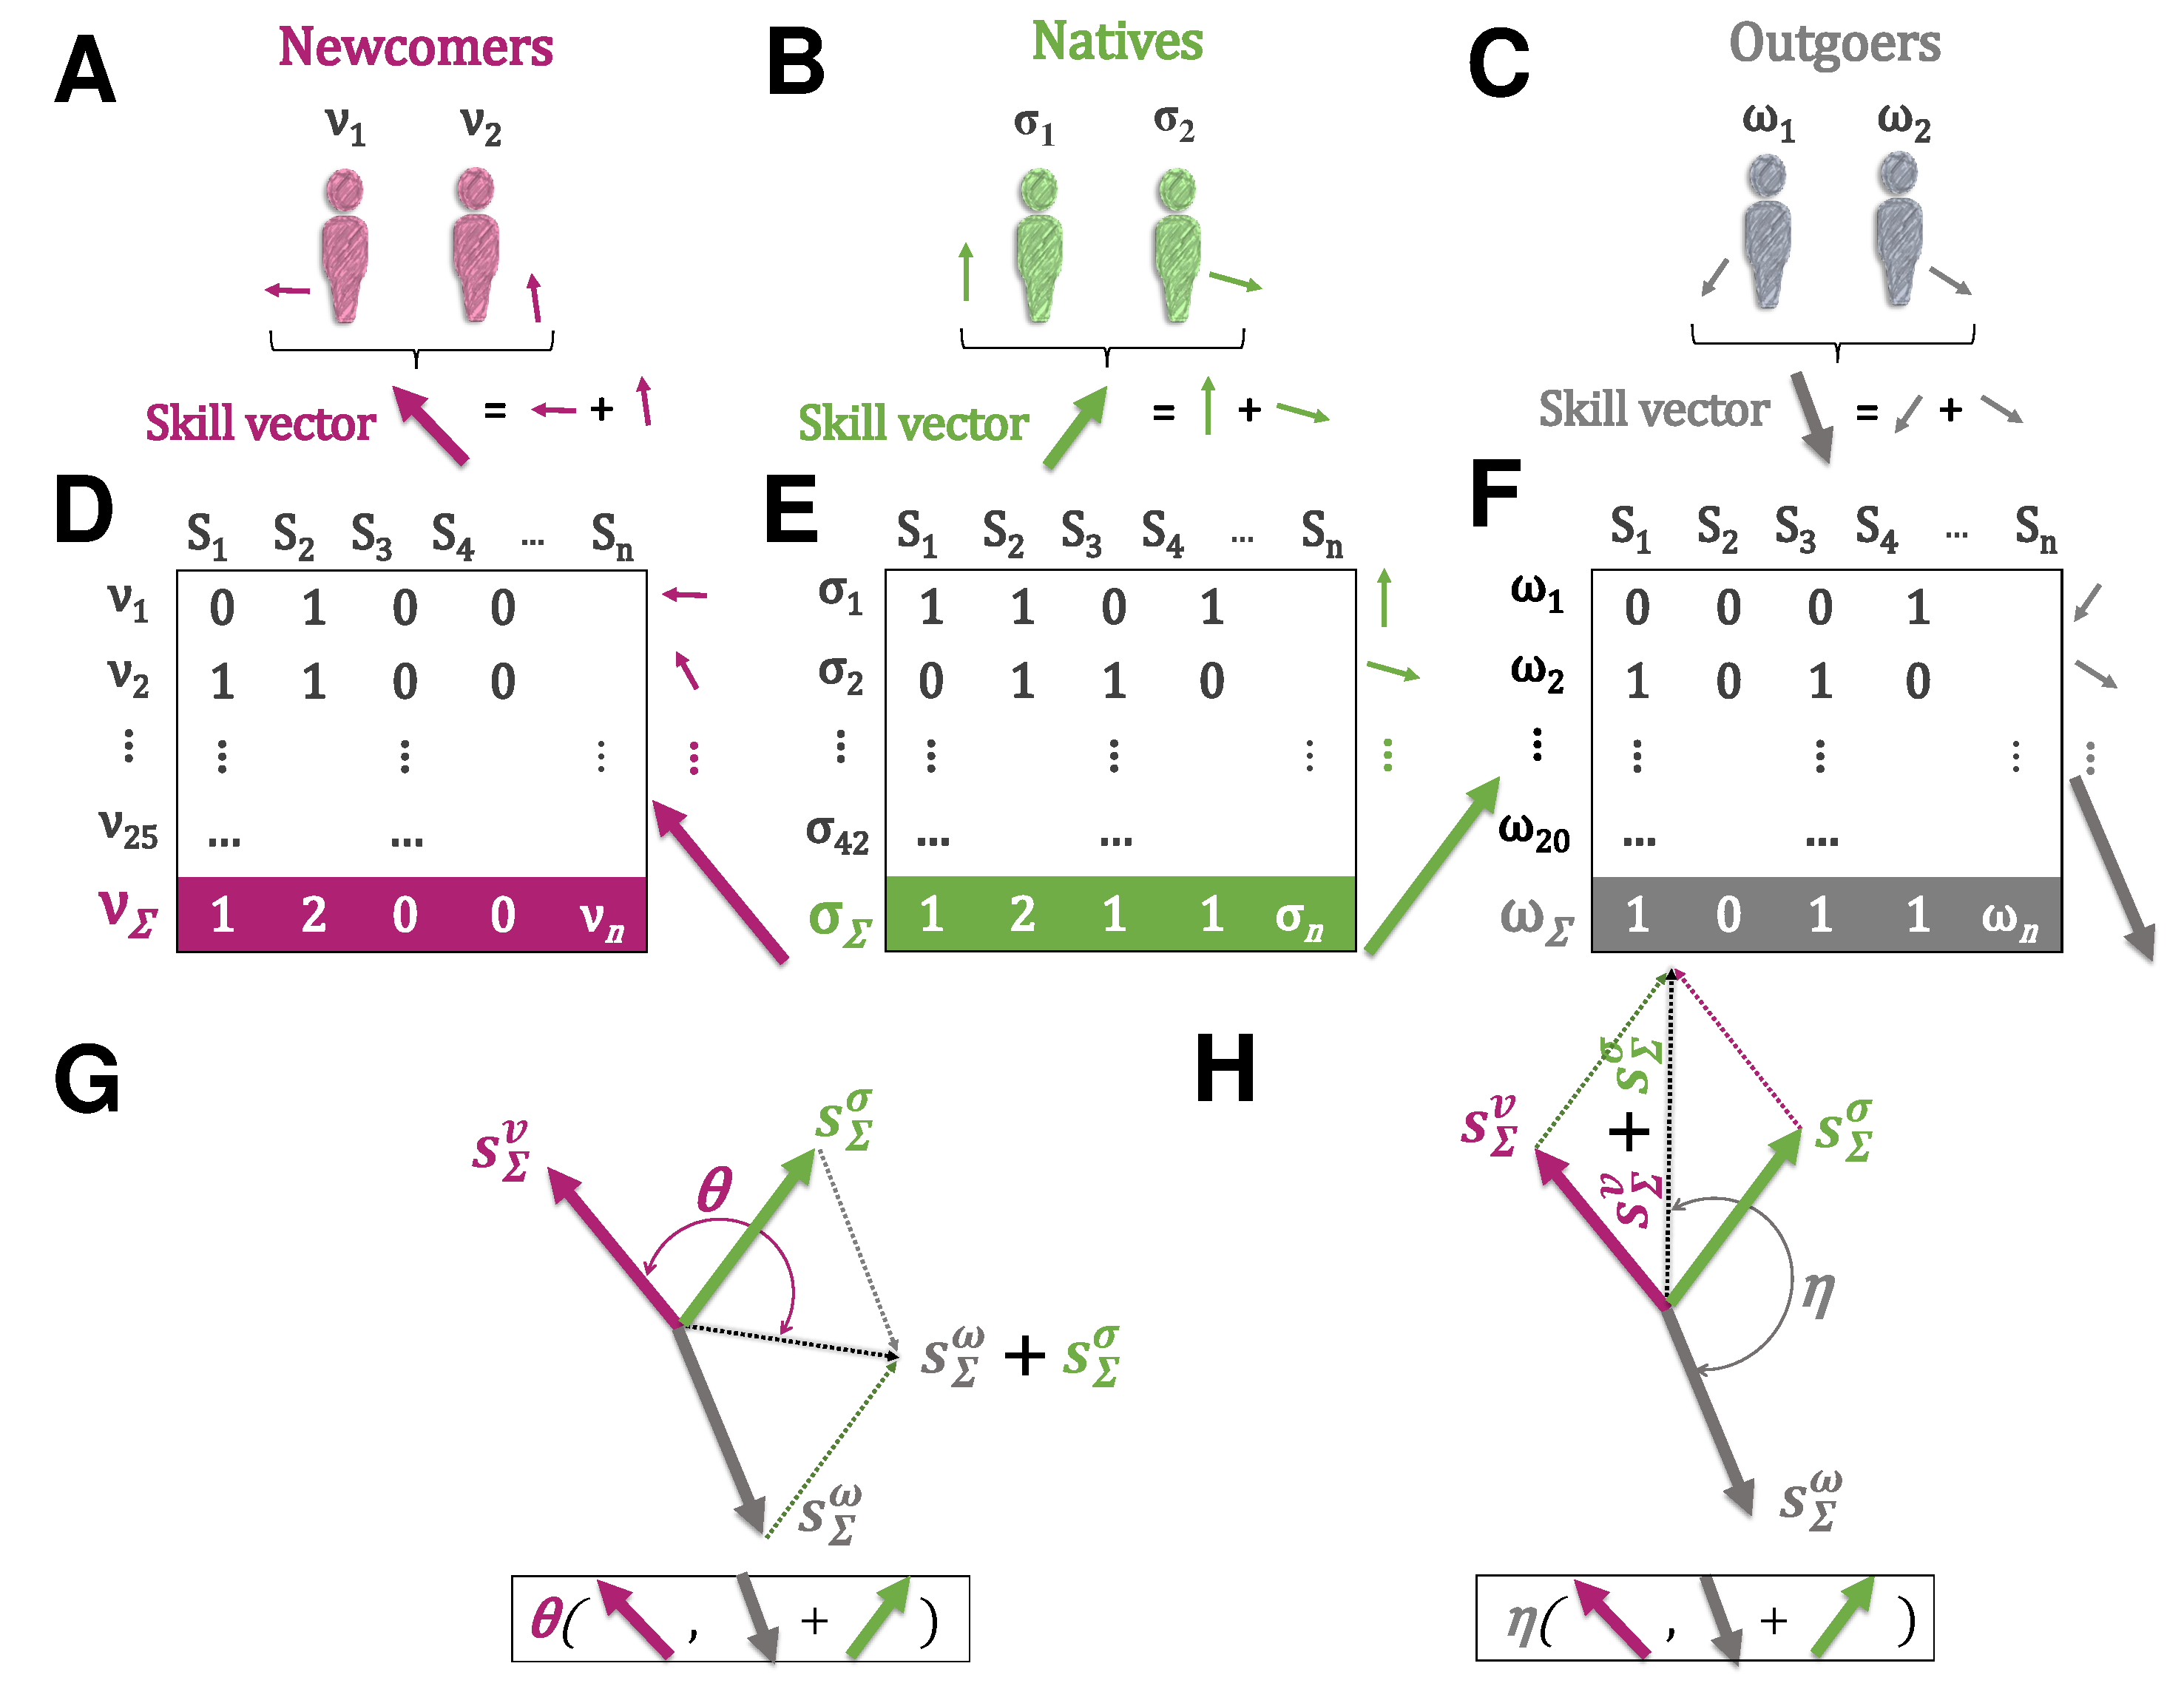
\includegraphics[width=0.95\linewidth]{figures_alignment/figure1abcdefgh_method.pdf}
\caption{A graphical representation of the skill and workforce structures of a scientific institution. We study three types of scientists (A, B, and C): \textit{institutional newcomers} $\nu$ (A), \textit{institutional natives} $\sigma$ (B), and \textit{institutional outgoers} $\omega$ (C). Every individual has a skill vector; every component in it, $S_k$, represents a particular skill $k$. We aggregate the individual skill vectors for each population (A), (B) and (C) of researchers and compute the cosine similarities between them, as shown in the grey boxes in panels G and H. We denote these similarities by $\theta$ (G) and $\eta$ (H). For illustration purposes, we took angles larger than $90\deg$.}
\label{Fig1:figure1abcdefgh_method.pdf}
\end{figure}

It has been argued that most academic institutions pursue the overarching goal of profile continuity \cite{heinze2008sponsor, march1991exploration} and that the long-term sustainability of institutions can only be achieved through various forms of alignment \cite{adams1996measuring}. Knowledge institutions typically invest and strengthen knowledge in their established research areas over time \cite{thurner2020role}, as leveraging on existing competencies can create alignments that improve performance, learning, and knowledge transfer~\cite{arthur1984competing, cohen1990absorptive}. When scientists within the institution have a common knowledge base, they can better learn from each other \cite{cohen1990absorptive}, leading to improved productivity and reduced barriers to collaboration. 

An important driver of attracting talent that matches the internal profiles of institutions is the current reward system of science \cite{merton1957priorities}. This system often and increasingly discourages the pursuit of novel research areas because the returns from new ideas and topics are seen as uncertain, distant, and often risky \cite{heinze2008sponsor}. In contrast, the benefits of refining and expanding existing expertise and technologies are positive, immediate, and predictable \cite{march1991exploration}. Other studies have suggested that too much similarity in knowledge can also limit innovation \cite{fleming2001recombinant}, which at the institutional level means that as academic organizations exceed optimal levels of alignment, they potentially `lock' into dominant thematic profiles.

The mobility of academic talent, collaboration, and the alignment of skill profiles between institutions and incoming and outgoing researchers can play a critical role in shaping research dynamics within and across institutions. However, on a quantitative basis, there is limited understanding of the processes behind the alignment of knowledge and skills within institutions and the alignment of the skills of institutions and new hires. To gain a better understanding of these alignment strategies, we study academic institutions from the perspective of the composition of their workforce and the internal skill profiles they generate as the composition of their workforce changes over time. 

We use the {\em Dimensions} database to compare the internal skill profiles of millions of mobile individuals with the skill structures of the institutions they move to or leave.
We quantify the academic skills of individuals by using their  publications mapped into a high-resolution classification scheme of scientific topics across all disciplines \cite{traag2019louvain}. This classification is the basis for defining the skill vector, $S^j$ for every individual, $j$. Every component of that binary vector represents a skill of the researcher, if the k-th component is $S^j_k=1$, researcher $j$ has competency $k$, if $S^j_k=0$, $j$ has no skill in $k$. If an author publishes in many different research areas, they has many `skills', if they publish on only one specific topic, the author has only a single non-zero component in the skill vector. The skills of an institution are defined as the superposition (sum of all vectors) of all the members of the existing workforce. These aggregated vectors are indicated as $S_\Sigma$, with a subscript $\Sigma$. The {\em Dimensions} database allows not only to quantify skills but also to observe the flows of researchers around the globe. 

However, measuring scientific skill profiles by bibliographic means is not an easy task. This partly depends on the level of resolution we use to determine researchers' skills. Data limitations have also been an obstacle to the study of scientists' knowledge pathways \cite{robinson2019many,sugimoto2017scientists, machavcek2022researchers}, leading to a prevalence of findings from self-reported information, small-scale studies, or studies limited to researchers from specific fields or countries \cite{jia2017quantifying,aleta2019explore, ganguli2015immigration, stephan2001exceptional, petersen2018multiscale, morgan2018prestige}. The situation is particularly problematic at the institutional level, as it relies on clear institutional identification and robust author-name disambiguation algorithms~\cite{donner2020comparing, machavcek2022researchers}. This situation has changed recently as more databases improve author and affiliation metadata \cite{robinson2019many,sugimoto2017scientists, machavcek2022researchers}. In what follows, we focus on harmonized research-intensive institutions data~\cite{hook2018dimensions,bode2018guide} for which extensive metadata on author-affiliation transitions exists~\cite{machavcek2022researchers}. 

In Fig.~\ref{Fig1:figure1abcdefgh_method.pdf}, we present a schematic view of how we approach the problem of skill assignment. We define three types of researchers: \textit{Newcomers} (A), \textit{Natives} (B), and \textit{Outgoers} (C). The natives represent the non-mobile workforce at a given institution, $i$. In the figure, we represent them as two scientists, $\sigma_1$ and $\sigma_2$, (green), both of which have different skills that are given by a skill vector, $S$, that has $n=4,163$ components that mark the different individual categories in the science classification scheme.  Native scientist $\sigma_1$ has three skills $S_1$, $S_2$, and $S_4$, hence $S^{\sigma_1}_1= S^{\sigma_1}_4= 1$, whereas $\sigma_2$ has only two, $S_2$ and $S_3$, $S^{\sigma_2}_2= S^{\sigma_2}_3= 1$, all other components being zero. Their combined skills are given by the sum of their skill vectors indicated by the small arrows. The skills present at the institution are seen in panel E. In this example, there are $r=42$ native researchers present; their skills are collected in the table. The sum of all their skills is called $S^{\sigma}_{\Sigma}$ and represents the current skill vector of the institution, $i$.  We now assume that in the next time period, a set of researchers will join the institution (newcomers, $\nu$) (A), and some will leave (the outgoers, $\omega$) (C). The collective skill vectors of these groups are called $S^{\nu}_{\Sigma}$ and $S^{\omega}_{\Sigma}$, respectively. In this example, we have 25 newcomers and 20 outgoers, with their skills captured in the tables in D and F. Data shows that the native population and newcomers make up the largest fraction in most institutions, while the outgoing population makes up the smallest fraction.

With this notion, we can now quantify the \emph{newcomer skill alignment} between the natives (plus outgoers) and the incoming workforce as the cosine of the angle, $\theta$, between the incoming skill vector, $S^{\nu}_{\Sigma}$ and the sum of natives and outgoers, $S^{\sigma}_{\Sigma}+S^{\omega}_{\Sigma}$; see panel (G). With this measure, we can analyze whether internally trained authors (natives and outgoers) and external authors (newcomers) generate aligned or divergent skill profiles at the institutional level. Similarly, we define the \emph{outgoer skill alignment} by calculating the cosine of the angle, $\eta$,  between the skill vector of outgoers, $S^{\omega}_{\Sigma}$ and the combined skill vectors of natives and newcomers, $S^{\sigma}_{\Sigma} + S^{\nu}_{\Sigma}$; see panel (H). 

% FIGURE 2 %
\begin{figure} [t] %[Overall trends and patterns]
  \centering
  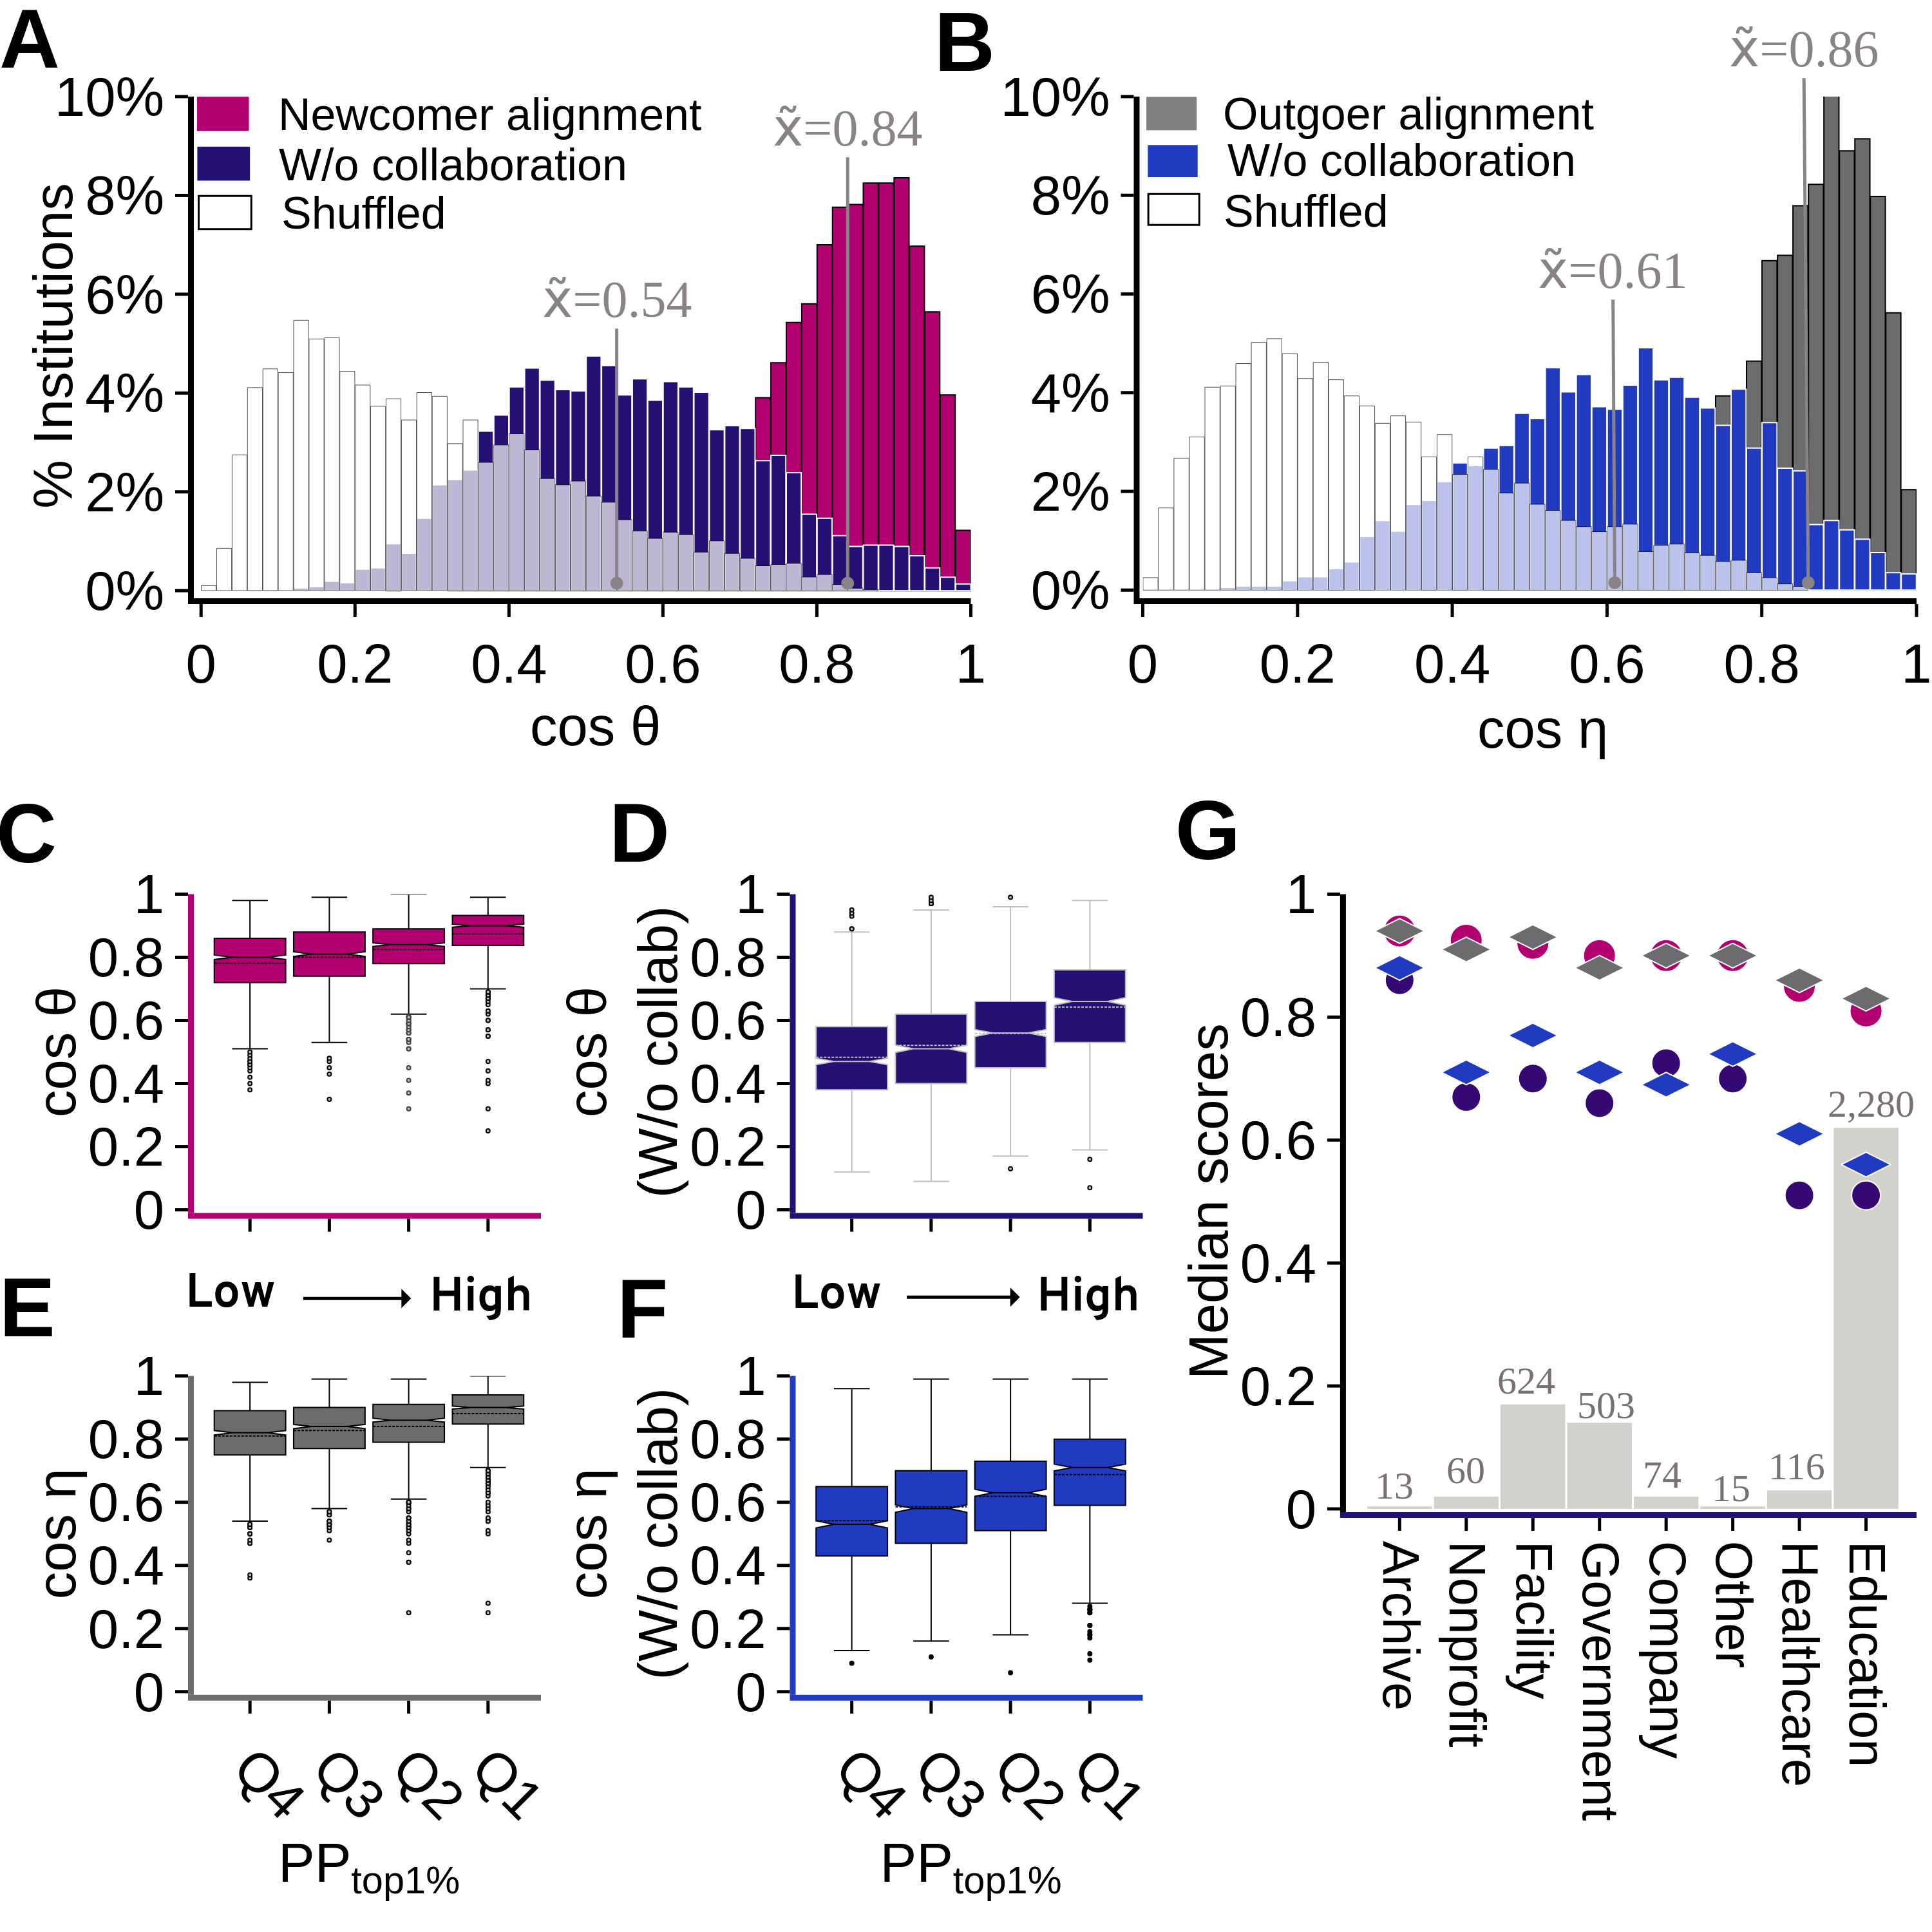
\includegraphics[width=0.7\linewidth]{figures_alignment/figure2abcdefg_new.png}
  \caption{Alignments of the skill profile of the native faculty and newcomers to- and outgoers from all academic institutions. Panels A and B show the distributions for newcomers, $\cos{\theta}$, and outgoers, $\cos{\eta}$, respectively. 
  The purple (panel A) and blue (panel B) distributions show the alignment of skills between those newcomers and outgoers that were not collaborating with their peers at the institution before they joined or during their stay, respectively. The transparent lines represent a reference distribution of skill alignments obtained by shuffling the target (source) affiliations of newcomers (outgoers) ($n=10,000$ random assignments). Clearly, skill similarity is absent in the shuffled data. Panels C, D, E, and F show the influence of the institution's reputation. The alignment is shown for the quartiles within the top 1\% most impactful institutions, {PP}$_{{top}1\%}$. The more impact, the more alignment, regardless of existing collaborations (compare C E and D E). Panel G captures the influence of institution type.
  It gives the median alignment scores by institution type. The shaded bars represent the percentage and number of institutions by organization type in our sample.~\label{fig2:figure2abcdefg_new.png}}
\end{figure}


\section{Quantifying the skills' profile of mobile scientists}
\label{Materials and Methods}
Investigating the alignment between the skills profile of mobile scientists (newcomers or outgoers) and that of resident faculty at the institutional level requires data that describes the skills of individuals and captures the temporal information of the affiliations of every scientist. Such information is typically unavailable in surveys on a country's labor force. 

Even if available, the categories of highly skilled workers are often too ambiguous to identify specific groups of scientists \cite{stephan2001exceptional}. Therefore, we use data from the {\em Dimensions}\footnote{{\em Dimensions} is produced by {\em Digital Science} and was launched in January 2018. For more references, see \href{https://www.dimensions.ai/}{Dimensions.ai website}} database, which we accessed through the Centre for Science and Technology Studies (CWTS) at Leiden University. {\em Dimensions} covers local journals more comprehensively than other large-scale bibliographic databases such as {\em Web of Science} or {\em Scopus}. Its broader scope allows our analysis to be more inclusive of organizations with a more local focus, and thus, we also reduce mainstream effects \cite{machavcek2022researchers, hook2018dimensions}. 

We examine the publication patterns of disambiguated authors from 108 countries between 2000 and 2020. Our analysis relies on three major improvements to the data: algorithmic disambiguation of author-names, improved consistency of organizations' metadata \cite{hook2018dimensions}, and a highly detailed field classification system \cite{traag2019louvain}, the latter also provided by the CWTS. We focus on disambiguated publications by authors with harmonized affiliation links. High-precision author disambiguation and institutional harmonization allow us to track the publication history of individual scientists across research institutions \cite{machavcek2022researchers}. This provides us with 9,299,250 million disambiguated author names.

Individual authors were disambiguated using the author-name disambiguation algorithm developed by {\em Dimensions} \cite{hook2018dimensions}, which uses the public ORCID\footnote{For more information, see \href{https://info.orcid.org/documentation/} {ORCID documentation}} as the basis for validating each author and their publication history. The disambiguation of organization names is based on the GRID \footnote{For more information, see \href{https://www.grid.ac/} { GRID website}} system \cite{bode2018guide}. For these authors, we retrieve their affiliations and publication history. We only consider publication-intensive institutions with at least 2,000 indexed publications, resulting in 3,965 institutions. Associated with these authors are 25,310,742 distinct documents indexed in the {\em Dimensions} database. The disambiguation of author names and the harmonization of research organization procedures allow us to produce a consistent overview of changes in researchers' affiliations with different institutions \cite{machavcek2022researchers} and topics in large-scale bibliometric analysis.

\subsection{Measures of skill alignment for scientific institutions}
\label{Definition of skills section}
The skill sets of an institution's workforce are defined using the publication-level classification system of science developed by Waltman and van Eck \cite{waltman2012new}. The classification is done using the Leiden algorithm 
\cite{traag2019louvain} that clusters publications based on direct citation relations. With this method, we obtain a  detailed classification system for scientific literature that covers all scientific fields. It provides several features. First, it identifies the relatedness between pairs of 38.4 million publications indexed in {\em Dimensions} that are directly linked to 513 million citation relations. This step processes publications such as articles, reviews, book chapters, and proceedings from 2006 to 2020. In the second step, the publications are clustered into research areas using a clustering procedure and the areas are organized in a hierarchical structure \cite{traag2019louvain}. Finally, the methodology results in a hierarchical clustering system: i) a top level with 22 broad disciplines, ii) the second level with 824 areas, and iii) the third level with 4,163 micro-clusters. For more details on this approach, we refer to \cite{waltman2012new, traag2019louvain}.

In this chapter, we consider the third classification level of 4,163 micro-clusters to define the skills profile vectors of institutions, as shown in Figure~\ref{Fig1:figure1abcdefgh_method.pdf}. In the figure, quantities with a subscript $\Sigma$ refer to the aggregate quantities of institutions. Formally, for an institution, $i$ (for which we have omitted the index $i$ in the figure for simplicity),
%
  \[ S^{\nu}_{\Sigma,i} = \sum_{r=1}^{N_i} S^{\nu_r}_{r,i} ~~,~~~ S^{\sigma}_{\Sigma,i} = \sum_{r=1}^{S_i} S^{\sigma_r}_{r,i} ~~,~~ S^{\omega}_{\Sigma,i} = \sum_{r=1}^{O_i} S^{\omega_r}_{r,i}
  \]
%  
where $S^{\nu}_{r,i},\ S^{\sigma}_{r,i},\ S^{\omega}_{r,i}$ represent the $n$-component skill cluster vector of the newcomer, native, and outgoer scientists, $r$, respectively. The institution where these scientists are hosted is labeled by the index, $i$.
The values $N_i,\ S_i,\ O_i$ represent the total number of newcomers, natives, and outgoers, respectively, in institution, $i$. 
Components in the skill vectors are always binary, $1$ if the skill is present, $0$ if it is not present in an individual or at the institutional level. 

The angles $\theta_i$ and $\eta_i$ are defined according to the cosine similarity expressions with the Euclidean dot product:
%
\begin{equation} \label{Eq.~1}
 \cos \theta_i = 
    \frac{S^{\nu}_{\Sigma,i}\cdot(S^{\omega}_{\Sigma,i}+S^{\sigma}_{\Sigma,i})}
        {|S^{\nu}_{\Sigma,i}|\, |S^{\omega}_{\Sigma,i}+S^{\sigma}_{\Sigma,i}|}. 
\end{equation}
%
\begin{equation} \label{Eq.~2}
   \cos\eta_i = 
        \frac{S^{\omega}_{\Sigma,i}\cdot(S^{\nu}_{\Sigma,i}+S^{\sigma}_{\Sigma,i})}
            {|S^{\omega}_{\Sigma,i}|\, |S^{\nu}_{\Sigma,i}+S^{\sigma}_{\Sigma,i}|}.
\end{equation}
%
These definitions quantify the skill profile alignment of newcomers, $\cos\theta_i$, and the skills profile alignment of outgoers, $\cos\eta_i$, relative to the remaining researchers at academic institutions. A value of $\cos\theta_i = 1$ (or $\cos\eta_i = 1$) indicates that two vectors of skill clusters are identical for a given institution, reflecting the fact that the institution attracts new scientists and retains native scientists or promotes outgoing scientists and retains native scientists with the same micro-clusters or `skills', but also that there are scientists producing publication outputs that express these skills with the same weight. Conversely, a value of $0$ means that these different types of scientists do not have the same skills profile. 

We introduce a reference or ``null'' model for these two measures that retains the size of the institutions in terms of their total number of competencies and the number of authors. This is done to remove correlations between newcomers (outgoers) and the profile of the natives. This way, we recalculate $\cos\theta$ and $\cos\eta$ by randomly assigning newcomers and outgoers to institutions. This procedure allows us to disentangle actual ''local'' matching between scientists from statistical effects due to collaborative activities and the institutional size; see Figure~\ref{fig2:figure2abcdefg_new.png}A and B.

Using the same workforce components shown in Figure~\ref{Fig1:figure1abcdefgh_method.pdf}, we additionally calculate a measure of inter-institutional skill alignment between institution $i$ and $j$, $\cos\phi_{ij}(t)$, to track whether institutions' profiles are aligning or diverging over time. 
Here, $\phi_{ij}(t)$ is the angle between total (native, incoming, and outgoing) skill vectors of institutions $i$ and $j$ at time period, $t$ (i.e., 2000-2004, 2005-2009, 2010-2014, and 2015-2019).
This indicator estimates and accounts for an institution's entire workforce (i.e., no distinction is made between newcomers, natives, and outgoers) and reflects overall profile alignment across all pairs of institutions over four non-overlapping time periods, $t$ . 

We define inter-institutional alignment, $\cos\phi_{ij}(t)$, as
%
\begin{equation} \label{Eq.~3}
 \cos \phi_{ij}(t) = \frac{T_i\cdot T_j}{|T_i|\,|T_j|} \, .
\end{equation}
%
where $T_i=S^{\nu}_{\Sigma,i}+S^{\omega}_{\Sigma,i}+S^{\sigma}_{\Sigma,i}$ is the combined total skill vector of all scientists at institution, $i$. Finally, we capture the change in pairwise institutional alignment, which we refer to as inter-institutional alignment, as
%
\begin{equation} \label{Eq.~4}
 \Delta \cos \phi_{ij}(t) = \cos\phi_{ij}(t+1) - \cos\phi_{ij}(t) \, .
\end{equation}

Clustering relatively homogeneous publication sets into high-resolution clusters allows us to compare the aggregate capabilities of scientists within and across institutions. As we explain in the following section, this allows us to compute the citation impact of organizations in a similar research context \cite{waltman2012new, ruiz2015field}.

\subsection{Citation impact indicators and normalization}
\label{impact indicators}
In recent years, in scientometrics, several changes took place that continue to influence the formal analyses of scientific dynamics. A growing awareness of the need to account for differences across and within disciplines when assessing the impact of research has increased research toward innovative indicators. In particular, field-normalized indicators based on bibliometric analyzes have become increasingly important for evaluating citation impact. For example, the average number of citations per publication varies significantly across scientific fields, institutions, and countries. The average number of citations per publication also varies by the age of the publication \cite{waltman2011towards}. Older publications are cited more frequently than more recent ones \cite{reisz2022loss}. Because of this uneven distribution of citations across different fields or years, citation counts or averages cannot be compared across research units \cite{waltman2011towards}. This is also important for the life and earth sciences, biomedical and health sciences, physical sciences and engineering, mathematics and computer science, and social sciences and humanities because these fields encompass different sub-disciplines and the sub-disciplines vary widely.

Taking these issues into account, we use the same high-resolution micro-clusters of topics used to define institutional competency vectors in \ref{Definition of skills section} - or the third level of classification and denoted by $S$ in \ref{Fig1:figure1abcdefgh_method.pdf} - to calculate the normalized citation indicators for each institution in our sample. These micro-clusters contain publications from multiple years (2000-2020), and each publication is assigned to a cluster based only on its citation relationships with other publications \cite{traag2019louvain}. We use a full-counting approach at the institutional level to calculate citation impact. That is, if two institutions contribute co-authors to a publication, the publication is counted as a full publication for both institutions. Using a full-counting approach, we give more weight to collaborative publications than non-collaborative ones~\cite{waltman2012new}. We use a publication window from 2006 to 2020 and a fixed citation window of four years to count citations to these papers through 2020. The authors' self-citations are not included in the calculation of impact indicators.

Before proceeding with the formal definition of citation-based indicators, we first consider a set of $n$ publications denoted by $1, \cdots, n$. Let $c_i$ denote the number of citations of a publication $i$, and $e_i$ denote the expected number of citations of publication $i$ given micro-cluster $S$ and year $t$ in which publication $i$ was published. In other words, $e_i$ is the average number of citations of all publications published in the same micro-cluster and year as publication $i$. We define two indicators of citation impact for each research institution: the {\em total normalized citation score}, TNCS, and the {\em proportion of publications in the top $n^{th}\%$}, PP$_\mathrm{top\,nth\%}$. The TNCS indicator captures an institution's total normalized citation rate of the produced publication volume. It is similar to what \cite{lundberg2007lifting} calls the total field normalized citation score indicator and is defined as
%
\begin{equation} \label{Eq.~5}
  \mathrm{TNCS} = \sum\nolimits_{i=1}^{n}\frac{c_i}{e_i} \, .
\end{equation}

%
The PP$_\mathrm{top\,nth\%}$ uses percentile rank classes instead of mean-based indicators to normalize the citation impact of publications \cite{bornmann2013use, waltman2012new, waltman2013calculation}. It measures the proportion of articles among the top $n^{th}$\% most cited papers in the same skill or micro-cluster, of the same age and document type. We first assign a percentile based on its position in the citation distribution of articles in the same micro-cluster. We use the approach described in \cite{waltman2013calculation} to calculate the percentile rank of each publication. In our analysis, we compute three variations of this metric. Specifically, we use the $99^\mathrm{th}$, the $95^{th}$ and the $90^\mathrm{th}$ percentile ranks, which assign papers with a percentile equal to or greater than the $99^\mathrm{{th}}$, $95^\mathrm{{th}}$, and $90^\mathrm{{th}}$ percentile to the top 1\%, 5\%, and 10\% of frequently cited papers, respectively. The percentile rank measures, PP$_\mathrm{top\,1\%}$, PP$_\mathrm{top\,5\%}$, and the PP$_\mathrm{top\,10\%}$ of each publication was calculated using
%
\begin{equation} \label{Eq.~6}
 \mathrm{ PP }_\mathrm{top\,x\%} = \frac{\sum_{i=0}^{\infty} n_i c_i} {\sum_{i=0}^{\infty}\ n_i} \, ,
\end{equation}
%
where $n_i$ denotes the number of publications from a scientific institution with $i$ citations. The score of a publication with $i$ citations is indicated by $c_i$. According to this definition, the PP$_\mathrm{top\,nth\%}$ is simply the average score of the publications of the unit of analysis. For simplicity, the definition assumes that all publications of a given unit belong to the same cluster. For more details, see \cite{waltman2013calculation, waltman2012leiden, waltman2011towards}. 

\section{Results}
\subsubsection{Skill Alignment in Research Institutions}
To what extent does the skills profile of externally trained incoming scientists match that of institutional natives? Do their skills align, or are they different? Figures~\ref{fig2:figure2abcdefg_new.png}A and B show the cosine similarity between the skills profile of the institutions and its newcomer and outgoing workforce. We find a substantial similarity with a median of $0.84$ and $0.86$ for the newcomers and outgoers, respectively. The fact that the skill alignment is slightly lower for the newcomers than for the outgoers suggests that the outgoers have become more similar in their skills while they stayed at the institutions. Panels A (purple) and B (light blue) also show the similarity between the existing workforce skills and the skills profile generated by those newcomers and outgoers who did not interact with the rest of the institution's workforce during their stay. For these cases, we find much less similarity (median $0.54$ and $0.61$). This indicates that internal collaboration is a potential driver of intra-institutional skill alignment. The regression analysis shown in ~\hyperref[SI4]{SI text 2} confirms that collaboration within institutions is an important predictor of intra-institutional skill alignment.

To illustrate that the observed alignments are a significant and genuine effect that does not simply emerge as a statistical consequence of the definition of the cosine-similarity measure, we devise a simple ``null model''. We preserve the skill profiles of the in- and outgoers but remove the correlations with the profiles of the institutions. We do this by randomly assigning newcomer and outgoer skill profiles to institutions. The distributions are shown as transparent lines in Figures~\ref{fig2:figure2abcdefg_new.png}A and B. The skill alignments practically vanish as a result. 

% FIGURE 3 %
\begin{figure} [!b] %[newcomer-outgoer corr]
  \centering
  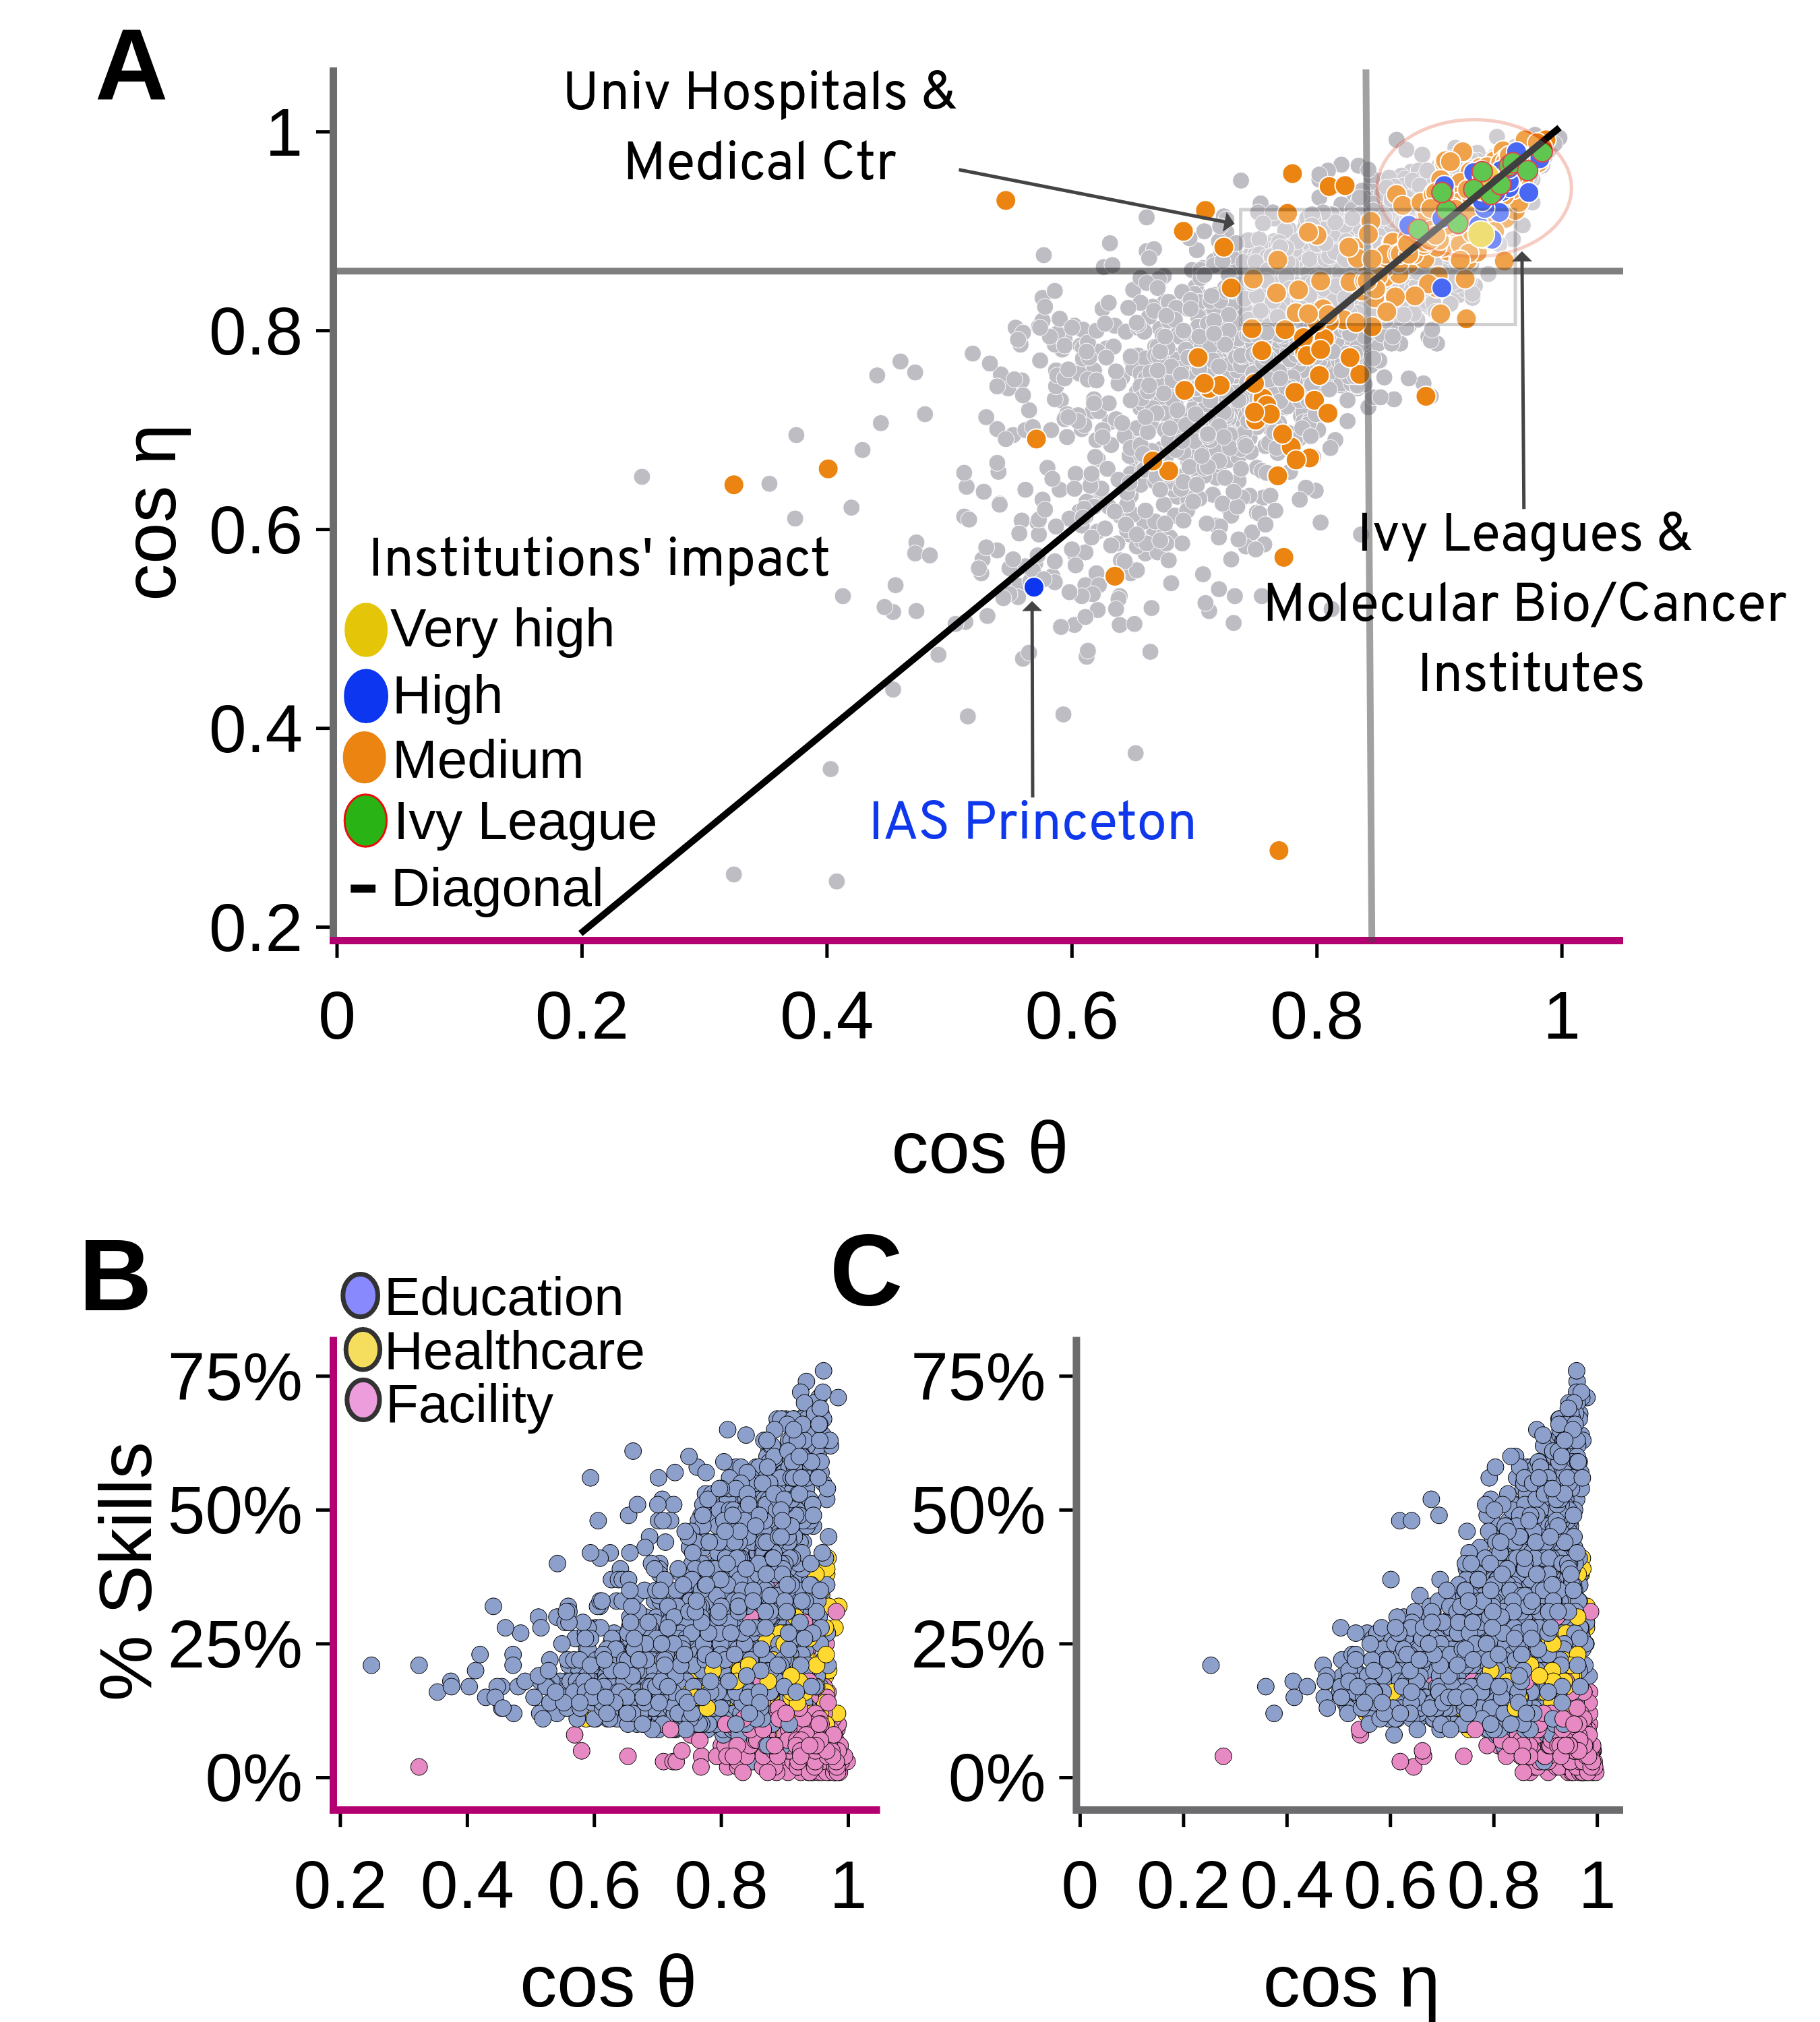
\includegraphics[width=0.7\linewidth]{figures_alignment/figure3abc.png}
  \caption{Scatter plot of the alignments of newcomers, $\cos{\theta}$, and outgoers, $\cos{\eta}$ (A). The line represents the diagonal (same in- and outgoer alignment). %the least squares fit (p$<0.001$, R${^2}=0.68$).
  The grey quadrant lines are positioned at the median values of $\cos{\theta}$ ($\tilde{x}=0.84$) and $\cos{\eta}$ ($\tilde{x}=0.86$). Every circle represents an institution. Color indicates the scientific impact of the institutions (${ PP }_\mathrm{top1\%}$ indicator). Grey institutions are below the global average (${ PP }_\mathrm{top1\%}\leq{0.01}$) of institutions with the same skills profile and years of production as explained in Materials and Methods section \ref{impact indicators}). Orange, blue, and yellow circles represent institutions with medium ($0.01\leq{ PP }_\mathrm{top1\%}\leq{0.05}$), high ($0.06\leq{ PP }_\mathrm{top1\%}\leq{0.09}$), and very high impact (${ PP }_\mathrm{top1\%}\geq{0.10}$), respectively. Top institutions tend to have generally high alignments and a slightly higher out-alignment. The scatter plots in panels B and C show the relation between the number of skills present at an institution (as a \% of all skills in the sample) and the skill alignments $\cos{\theta}$ (B) and $\cos{\eta}$ (C) for Education, Healthcare, and Facility research institutions, respectively. Healthcare and Facilities tend to have high in- and out-alignments; see also~\hyperref[SI]{SI}~Figure~\ref{SI:figure3abc_wo_collaboration.png}.}
  \label{fig3:figure3abc.png}
\end{figure}

There is a clear relation between institutional prestige, as captured by the {PP}$_\mathrm{top1\%}$ indicator (for definition, see  Materials and Methods \ref{impact indicators}), and skill alignment. Figures~\ref{fig2:figure2abcdefg_new.png}C and E show that institutions that have substantially more than one percent of their publications in the top 1\% most cited papers worldwide tend to have similar skill profiles across the different types of workforce. Newcomers who move to an institution with top-cited publications tend to have more similar skill profiles than newcomers who move to a less prestigious institution, see C. The situation is similar for departing scientists, see E. In other words, talent flowing to and from organizations with high institutional prestige is associated with greater skill alignment. A greater skill dispersion is also observed at universities with lower prestige. If we compare C with D and E with F, we see that the prestige effect is independent of whether there are collaboration ties (i.e., co-authorship) between newcomers and outgoers with local researchers.

Figure~\ref{fig2:figure2abcdefg_new.png}G shows the median alignment between newcomers and outgoers (colors correspond to those in panels A and B) and institutional natives by organization type. More generalist educational institutions (e.g., universities) tend to have lower median levels of similarity than more thematically focused institutions such as Facilities, Archives, Companies, Non-profits, or Governmental institutions. Interestingly, Healthcare research institutions also show comparatively low median scores of alignment, which may indicate that while they are considered specialized, their skill sets are broad enough to encompass a greater diversity of skill profiles between in and outgoing researchers and natives.

Figure~\ref{fig3:figure3abc.png}A shows the alignment of newcomers (x-axis) versus the alignment of outgoers (y-axis). The color indicates the degree of the citation's impact of institutions. The solid line marks the regression result. We segment the plot into four quadrants (gray lines at the median alignment values) associated with strategic patterns of talent attraction and training. Institutions (41\%) in the first quadrant (top right) attract and send the same skills at a rate above the median. Most notably, the U.S.\ Ivy Leagues, top European universities, and prominent molecular biology and cancer research institutes are in the first quadrant. There we also find several university hospitals and medical centers. This indicates that the institutions' strategy in the first quadrant is thematic continuity \cite{heinze2008sponsor, march1991exploration} and homogeneity in their recruitment and training practices. 

In the third quadrant (bottom left), we observe the opposite trend for about 45\% of institutions. Here, the profiles of newcomer hiring and outgoing researchers within an institution diverge and fall below the overall median scores. An example of this pattern is the Institute for Advanced Study (IAS) at Princeton (blue circle). This institute has a remarkably low alignment between outgoers and the rest of the institution, as well as between newcomers and the rest of the institution. Historically, the IAS has been a place where scientists retreat for sabbaticals and exchange ideas, encouraging unexpected discoveries and interdisciplinary thinking. This suggests that it is not always necessary to have a high-skill alignment of newcomers and outgoers to conduct high-impact research. Our method captures their (non) alignment strategy. However, IAS is an exception since this strategy seems prevalent at most institutions whose citation performance is below or close to the global average (grey).

The second quadrant (upper left) shows institutions (8\%) that attract researchers working in potentially complementary research areas. These institutions send researchers who produce skill-aligned profiles above the median of the other institutions to the institution's facilities and attract those who produce differentiated work below the median to the rest of the institution. In the fourth quadrant (bottom right), we find the opposite situation; about 6\% of institutions bring more of the same skills and send more researchers who exhibit different skills.
 
In Figures~\ref{fig3:figure3abc.png}B and C show the number of skills present at an institution (in \% of all possible 4,163 skills in our classification, see Materials and Methods section \ref{Definition of skills section}), versus the skill alignment at institutions, B newcomers, C outgoers. We find considerable heterogeneity. Colors highlight three types of organizations: Education, Healthcare, and Facility, which account for 93\% of the institutions in our sample. The education category includes general and specialized universities, while the healthcare category includes university hospitals and medical research centers. Facilities, typically  established by the government or academic stakeholders, often specialize in one particular field, such as agriculture, high-energy physics, specific technologies, and others. We see that research facilities tend to be more specialized (small percentage of skills) and have higher skill alignments of both their incoming (B) and outgoing (C) workforce. Educational institutions tend to have a larger number of skills and show a large spread in both number of skills and alignment. Healthcare institutions fall between the two regarding skill diversity and show relatively high alignment values. 

In~\hyperref[SI4]{SI text 2}, we conduct a multivariate regression analysis that examines the relationship between alignment and scientific impact measures and various controls while considering the different sizes of institutions. Our findings indicate that the level of internal collaboration within an institution and citation impact are important factors in determining skill alignment within academic institutions. 

% FIGURE 4 
\begin{figure}[!ht] %[field differences]
\centering
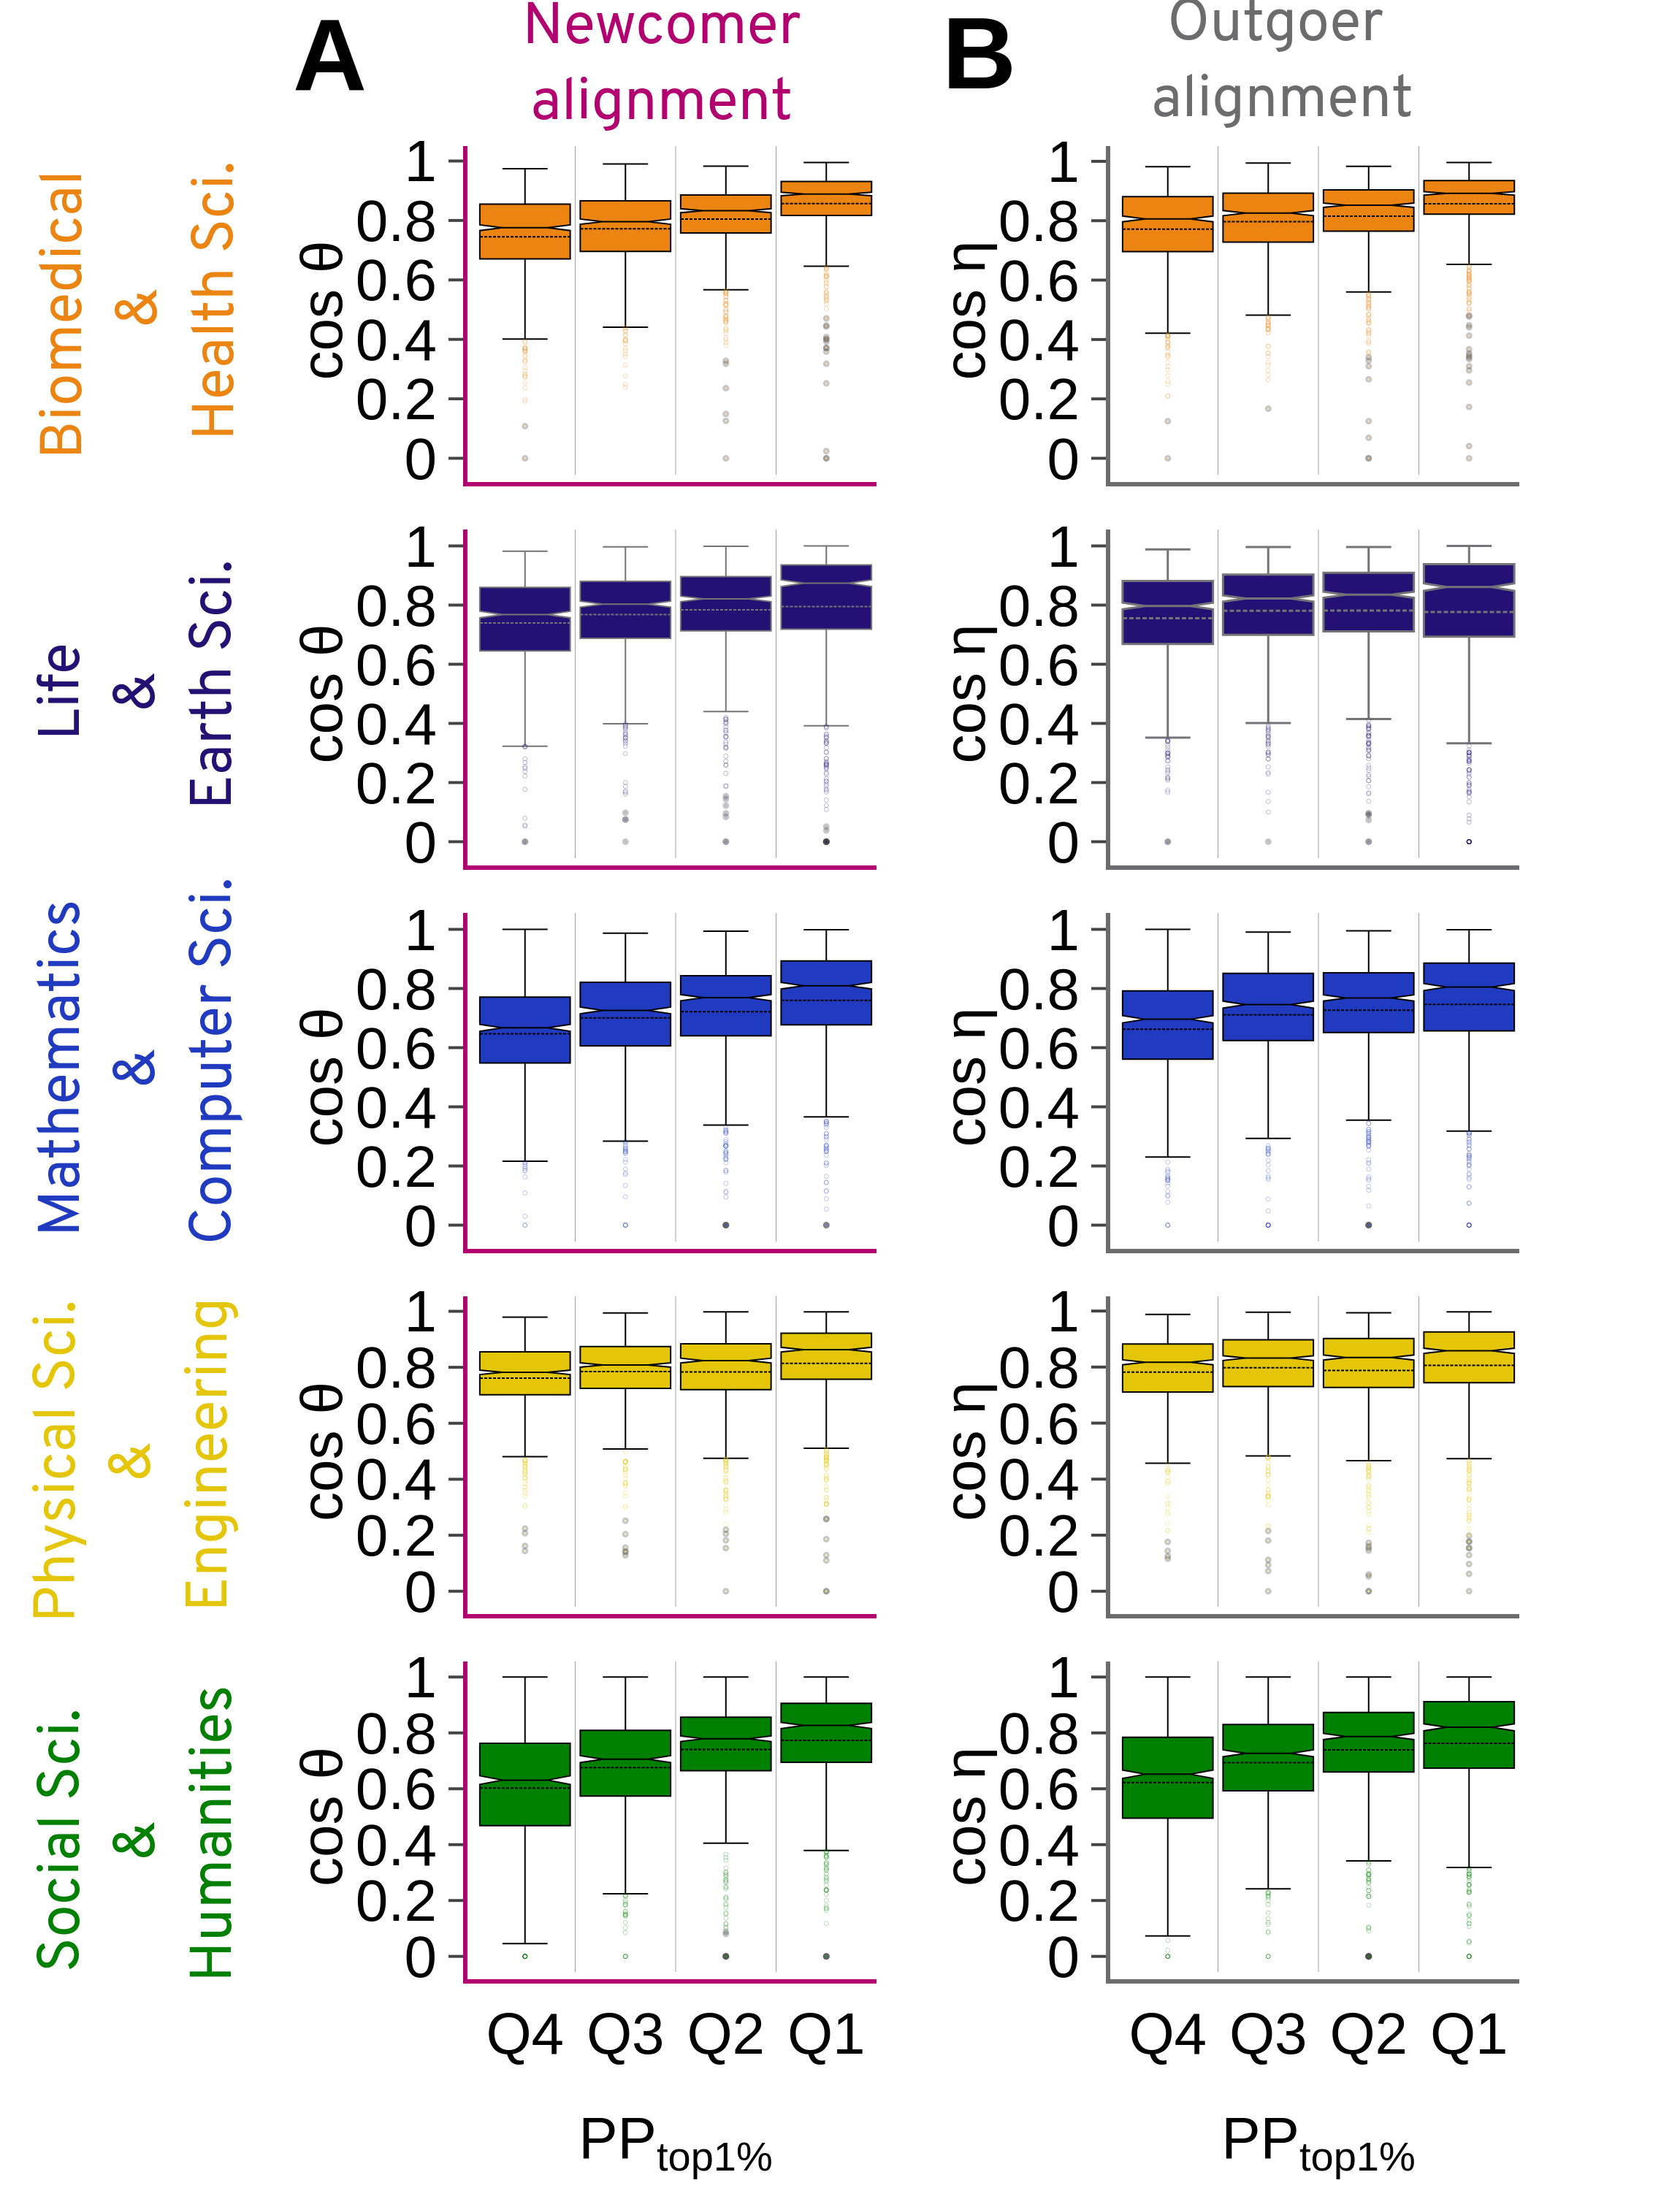
\includegraphics[width=0.7\linewidth]{figures_alignment/figure4ab.png}
\caption{Skill alignment of newcomers (A) and outgoers (B) 
in five main scientific fields as  a function of  institutional prestige as captured by impact quartiles of PP$_\mathrm{top1\%}$ (same figure setup as in Fig \ref{fig2:figure2abcdefg_new.png} C and E). Again, top-cited institutions have higher newcomer and outgoer alignment than average organizations (two-sample $t$ test, $P$ value <0.001). Disciplines are arranged alphabetically from top to bottom.
Social sciences, humanities, mathematics, and computer science show lower levels of alignment than biomedical and health sciences, life and earth sciences, physical sciences and engineering.
For the case controlled for collaborations, see  \hyperref[SI]{SI}~Figure~\ref{SI:figure8ab.png}.}
~\label{fig4:figure4ab.png}
\end{figure}

\subsubsection{Skill Alignment in Different Science Fields}
Various degrees of skill alignment are found in the five major areas of science. Figure~\ref{fig4:figure4ab.png} shows a breakdown of the distribution of alignment scores for newcomers (A) and outgoers (B). We find that the profiles for academics in the social sciences, humanities, mathematics, and computer science show lower levels of alignment. This is especially true for lower impact institutions, as captured by the quartiles of the proportion of papers in the top one percent (PP$_\mathrm{top1\%}$ indicator). Finally, in the fields of biomedical and health sciences, life and earth sciences, and physical sciences and engineering, there is a comparatively slightly higher degree of similarity between the skills of newcomers with their institution as well as between outgoers and the rest of their institution.

\subsubsection{Skill Alignment Between Academic Institutions Over Time}
Finally, we present the situation of the alignment of skills between all the institutions in the sample. We analyze the  inter-institutional skill alignment, i.e., the similarity of skill profiles of the entire workforce of institutions between all institutions in the sample. The inter-institutional skill alignment is defined as the skill profile similarity denoted by $\cos{\phi}$ (see Materials and Methods section~\ref{Definition of skills section} for the definition). We compute it for all pairs of institutions. Figure~\ref{fig5:figure5ab.PNG}A shows average inter-institutional skill alignment during four time periods from 2000 to 2019. The red error bars mark standard errors of the mean. We see that the average skill alignment is generally low, however, it doubled in the past twenty years, i.e., across the globe, skill profiles of institutions have become more similar. 

% FIGURE 5 
\begin{figure} [!ht] %[University-wise panel sim]
\centering
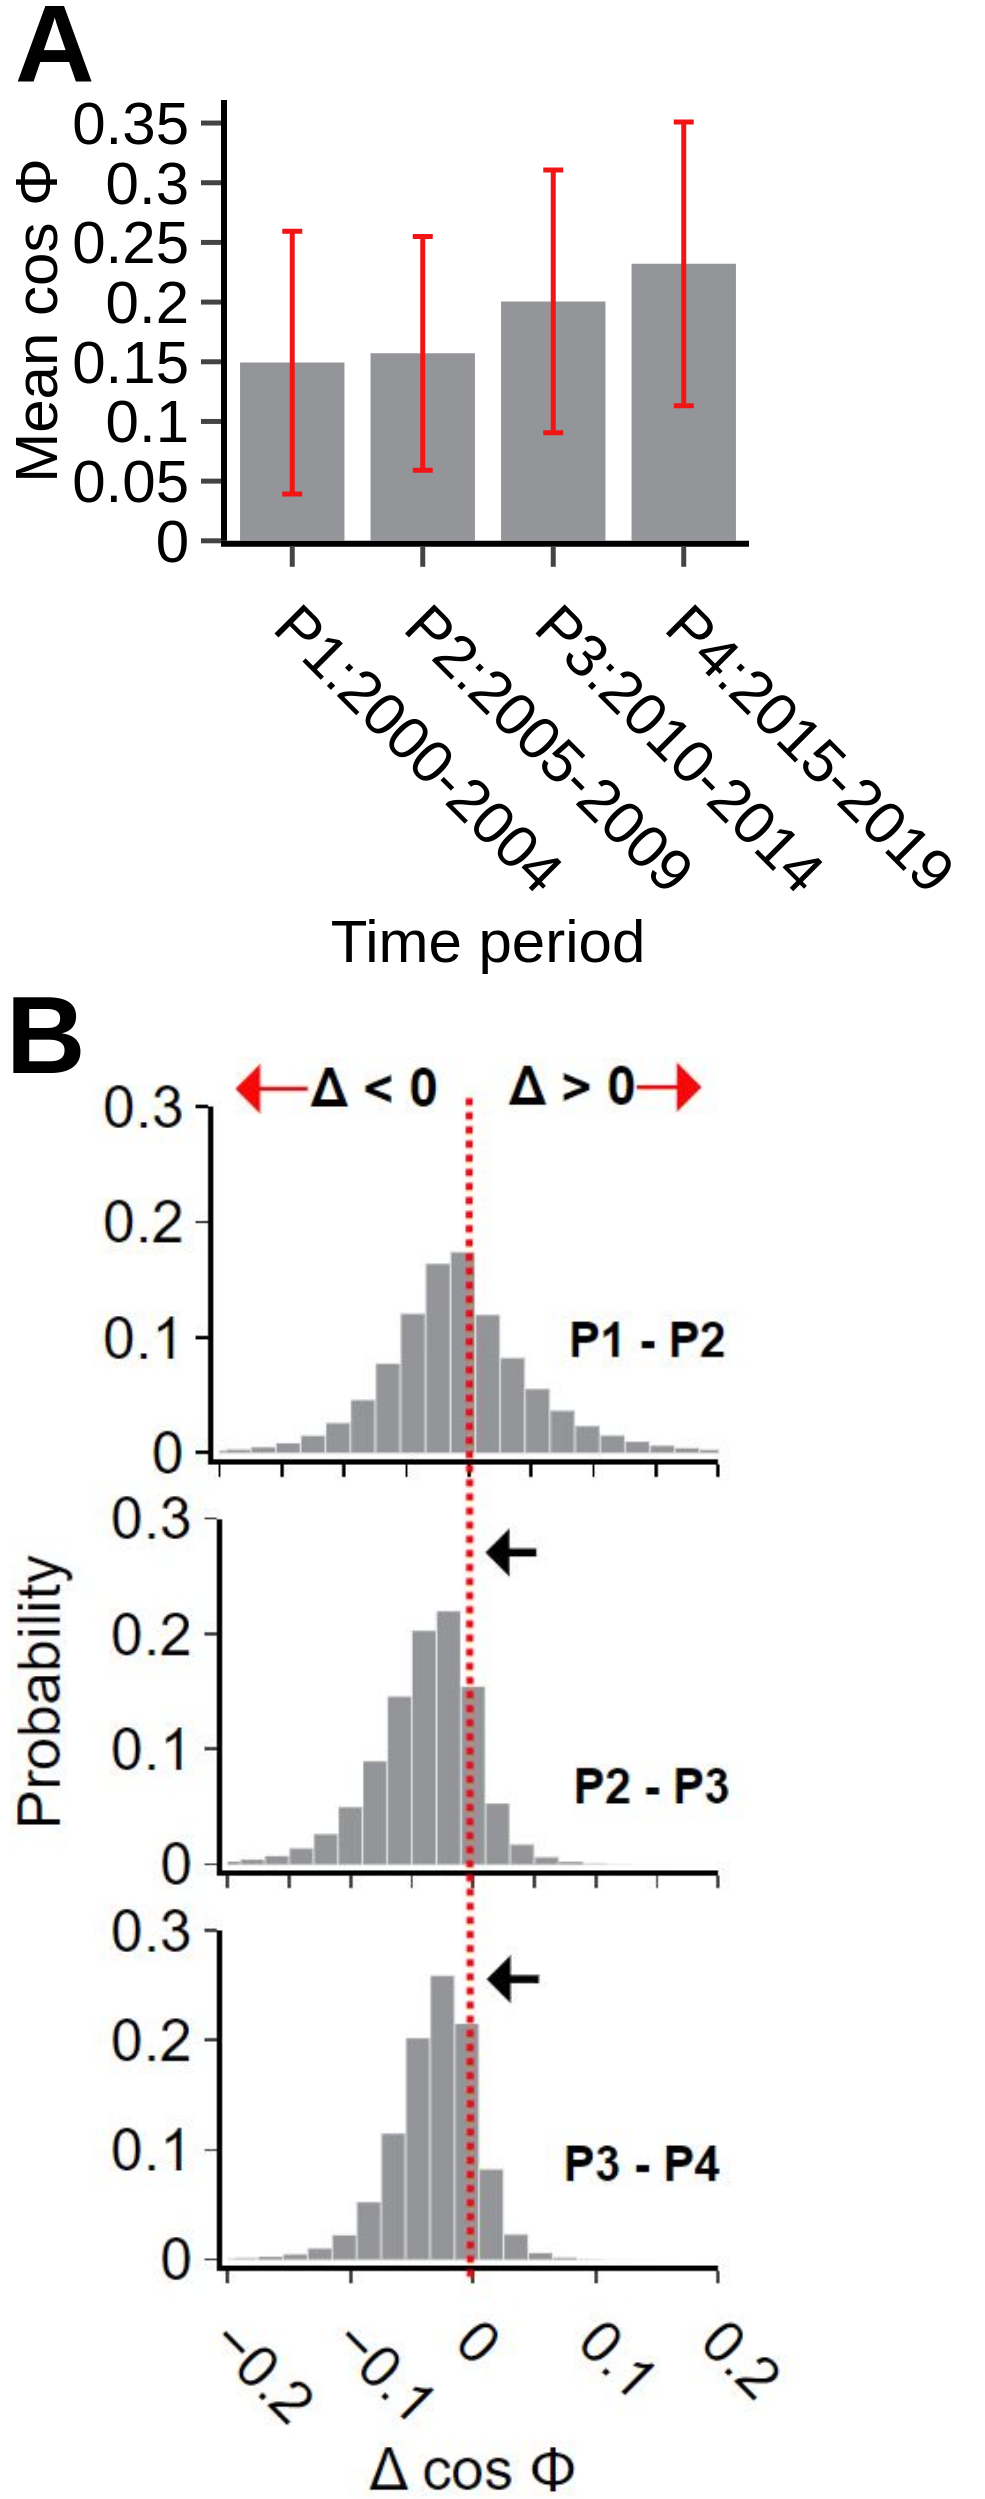
\includegraphics[width=0.4\linewidth]{figures_alignment/figure5ab.PNG}
\caption{Inter-institutional skill alignment over time. Panel A shows the average of pairwise cosine similarity for all pairs of institutions for four non-overlapping time periods: P1:2000-2004, P2:2005-2009, P3:2010-2014, and P4:2015-2019. The red error bars represent standard errors. Panel B shows the differences between the overall skill alignment of pairs of institutions, $\Delta\cos{\phi}$, over time. $\Delta<0$ means that institutions become increasingly similar in the composition of their overall skill profiles. The sub-panels capture the changes between the time periods. The tendency of becoming more similar is visible (over time, the peak is moving to the left).}
\label{fig5:figure5ab.PNG}
\end{figure}

Figure~\ref{fig5:figure5ab.PNG}B shows the distribution of the differences in skill alignment between the pairs of institutions over time. A value of $\Delta \cos{\phi}$  below zero means that institutions have become more similar; when $\Delta \cos{\phi} >0$, institutions become more dissimilar. The dashed red line indicates the zero line of the x-axis. The three sub-panels capture the changes between the time periods, P1-P2, P2-P3, and P3-P4. It is visible that the peak of the distribution is moving toward the leftover time, indicating an acceleration toward becoming more similar in more recent years.

\section{Discussion}
By quantifying the alignment of skills present at $3,965$ institutions, which includes the publication records of $9,299,250$ disambiguated authors affiliated with $108$ countries, with the $4,163$ skill types of the incoming and outgoing workforce, we can show strong quantitative signatures of academic skill alignment -- the degree to which mobile scholars (newcomers or outgoers) publish on topics that are in line with those of their colleagues already at the new institution. In particular, newcomers tend to publish on topics that align with those of their colleagues already at the new institution. Alignment, as measured by skills profile similarity, is more pronounced at the most prestigious (i.e., top-cited) institutions than at average institutions. Even within the top 1\% of highly cited institutions, there is a correlation between skill alignment and institutional citation performance. Research institutions with moderate levels of citation impact tend to have significantly less aligned skill profiles between natives and in- and outgoers. The greater alignment of skill profiles at top institutions is not surprising, as it indicates a strategic, specific, and targeted hiring policy that may not be present at more moderate institutions.

Highly aligned skill profiles potentially realize synergies between newcomers and existing faculty \cite{arthur1984competing, cohen1990absorptive} and can reinforce already strong research portfolios. However, this also may lead to selection pressures for those hired and the hiring institutions themselves and eventually lead to the under-representation of relevant research expertise, and important topics \cite{evans2014attention}. 

Two likely mechanisms could explain the origin of the observed similarities. One is that the newly hired scholars adapt their publication behavior (and scholarly interests) to the existing academic interests of the new institution. In this work, we see evidence that this may be the case, the outgoing researchers are more similar to the natives than the incoming researchers. This is reflected in a shift toward higher alignment and a narrower alignment distribution among outgoers. The other mechanism is the preference of institutions to hire scholars with similar skills to their current knowledge base or the preference of scholars to move to universities that are established in their fields. Also, a preferential dynamics of researchers going to places where lots of expertise exists, as, e.g. described in \cite{vitomarcia22}, might explain part of the observed effects. 

We also assessed the role of collaboration within the institution. We found a significant difference in the skill alignments of newcomers who have collaborative relationships (co-authorship on publications) with colleagues (natives or outgoers) at hiring institutions. Our results suggest that collaboration is the most natural approach for newcomers and natives to align, combine, and complement their skills at the institution. Both newcomers and outgoers who did not engage in collaborations are virtually unmatched by the local workforce, i.e., the cosine $\sim 0.5$. Note that skill differences between natives and newcomers are small when the degree of cooperation between them is high. The role of collaboration in skill alignment may also explain the disciplinary differences observed in our study, where Social Sciences, Humanities, Mathematics, and Computer Science show systematically lower levels of skill alignment. These disciplines traditionally have lower collaboration rates than the Natural Sciences or Engineering \cite{gazni2012mapping}.

A shortcoming of the present work is that individual preferences and motivations for mobility cannot be assessed. It would be interesting to supplement these results in future work with appropriately designed surveys and controlled experiments to uncover the relative importance of the individual-level mechanisms that lead to the observed profile alignments at the institutional level.

The presented results on the extent of skill alignments in scientific hiring can be considered steps toward a better understanding of talent flows in science. Future research would be important to determine how the alignment of institutions' skills profile interacts with different dimensions of workforce diversity, such as gender and seniority. This could provide policymakers with analytical tools to uncover the latent capabilities of different kinds of newcomers and assess their ability to influence (or not) the skill profile of their institutions.

Quantitative measures, such as those presented here, can inform and evaluate university (and unit) policy regarding their mobility, recruitment, and talent acquisition strategies, particularly about their existing competency profiles and those desired in the future. University leadership, funding agencies, and science policymakers in general-- may benefit from a quantitative assessment of the degree of alignment within their respective areas or organizations and can use it to develop interventions aimed at reaching desired alignment levels (e.g., by promoting internal collaboration networks). 

\newpage

\section{Supplementary information~\label{SI}}


\begin{figure} [!ht] %SI Figure Similar setting as Figure 3 in Main Text
\centering
  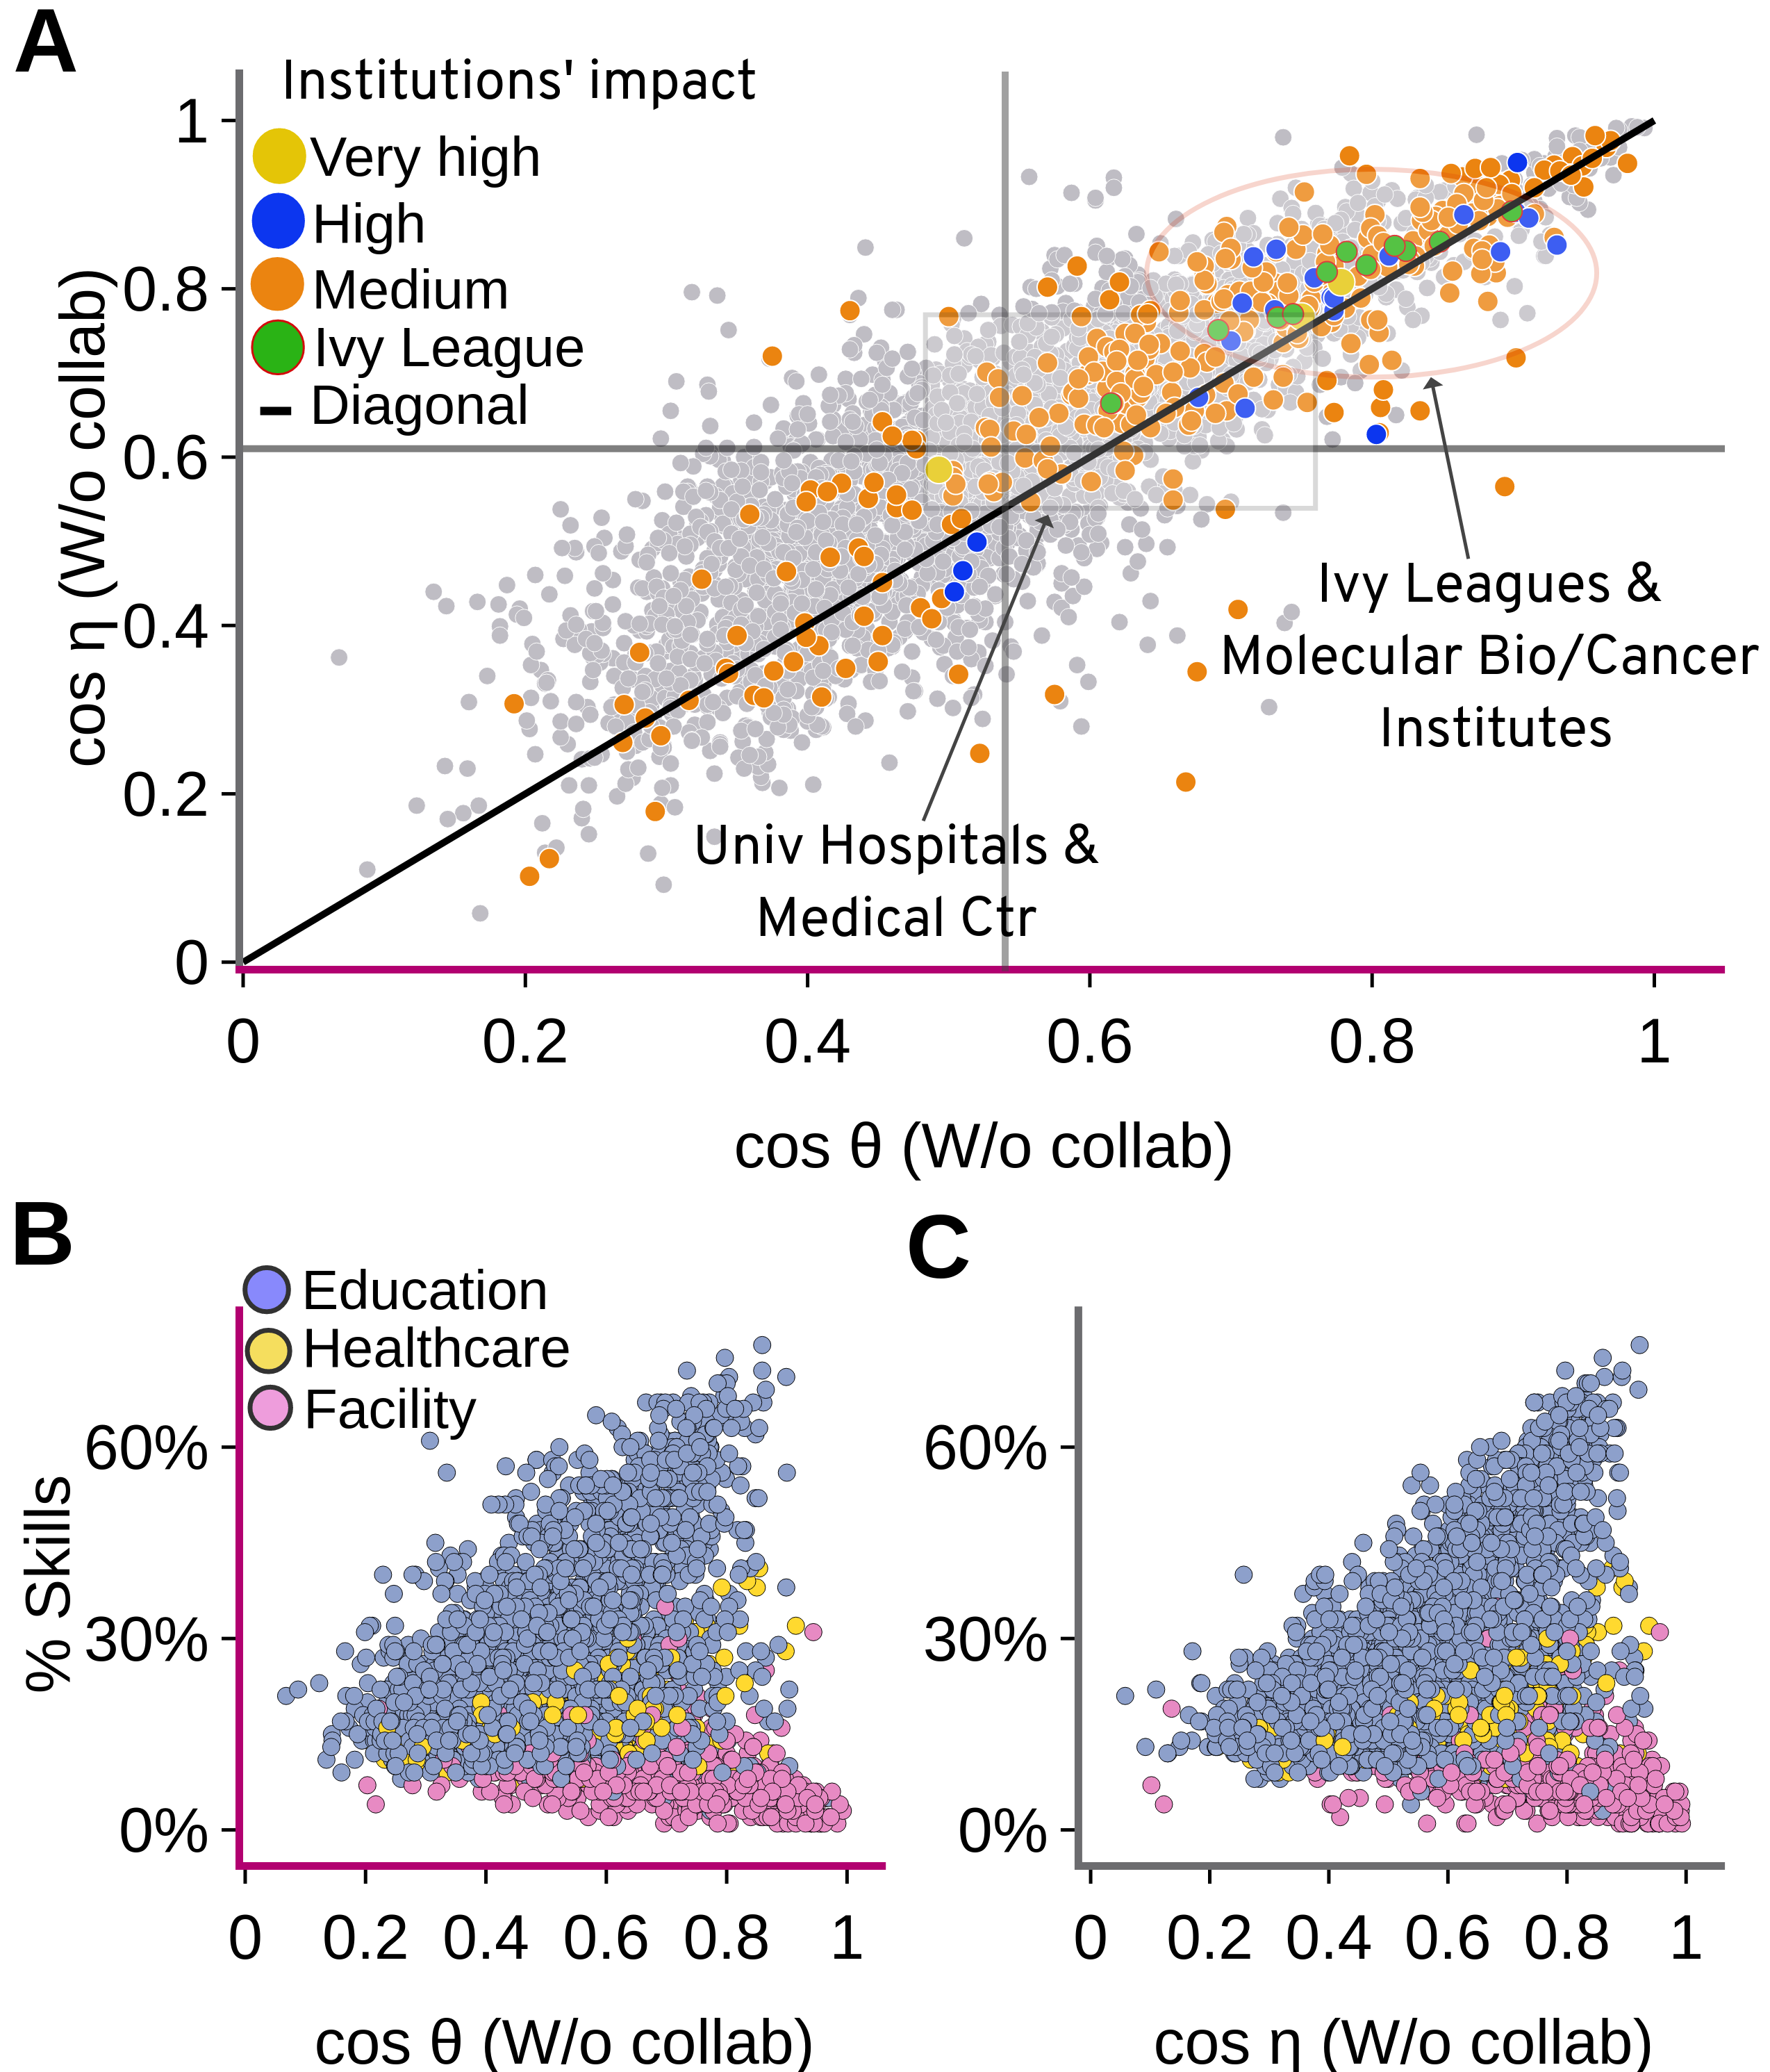
\includegraphics[width=0.5\linewidth]{figures_alignment/figure3abc_wo_collaboration.png}
\caption{Scatter plot of the correlation between newcomer $\cos{\theta}$ (W/o collab)- and outgoer $\cos{\eta}$ (W/o collab) alignment measures.Grey quadrant lines of median $\cos{\theta}$ (W/o collab) ($\tilde{x}=0.54$) and $\cos{\eta}$ (W/o collab) ($\tilde{x}=0.61$) are shown. Each circle in A represents an institution. The color of the circles represents the scientific impact of the institutions as captured by the PP$_\mathrm{top\,1\%}$ indicator. Grey-colored institutions have a PP$_\mathrm{top\,1\%}$ that is close to or below the global average (PP$_\mathrm{top\,1\%}\leq{0.01}$) of institutions with the same skill profile and years of production. The orange, blue, and yellow circles represent institutions with medium ($0.01\leq \mathrm{PP}_\mathrm{top\,1\%}\leq{0.05}$), high ($0.06\leq\mathrm{PP}_\mathrm{top\,1\%}\leq{0.09}$), and very high impact (PP$_\mathrm{top\,1\%}\geq{0.10}$). 35\% of institutions are in quadrant 1, 29\% in quadrant 2, 36\% in quadrant 3, and 1\% in quadrant 4. The scatter plots in panels B and C show the relationship between an institution's percentage of its total skills and $\cos{\theta}$ (W/o collab) and $\cos{\eta}$ (W/o collab), respectively, for education, health, and research facilities when articles in collaboration between the different types of the workforce are excluded. The panels have the same setting as the Figure~\ref{fig3:figure3abc.png}, but this time for the measures $\cos\theta$ (W/o collab) and $\cos\eta$ (W/o collab), i.e. for the case of non-collaborative hires and leavers. We find much greater variability than in the main measures of skill alignment in the main text. Similar to Figure~\ref{fig3:figure3abc.png}, the skill profile of newcomers and outgoers is concentrated in the first and third quadrants, followed by the second and fourth quadrants. Interestingly, ``Ivy League'' universities and molecular biology and cancer research institutes remain concentrated in the first quadrant. In contrast, university hospitals and medical research centres are mainly found in the second and first quadrants. The most frequently cited institutions are mostly concentrated around high scores for non-collaborative alignment in quadrant one, with some exceptions spreading across the other three quadrants. Panels B and C show a very similar trend compared to figures~\ref{fig3:figure3abc.png}B and C.
}
\label{SI:figure3abc_wo_collaboration.png}
\end{figure}


\begin{figure} [!ht]
\centering
  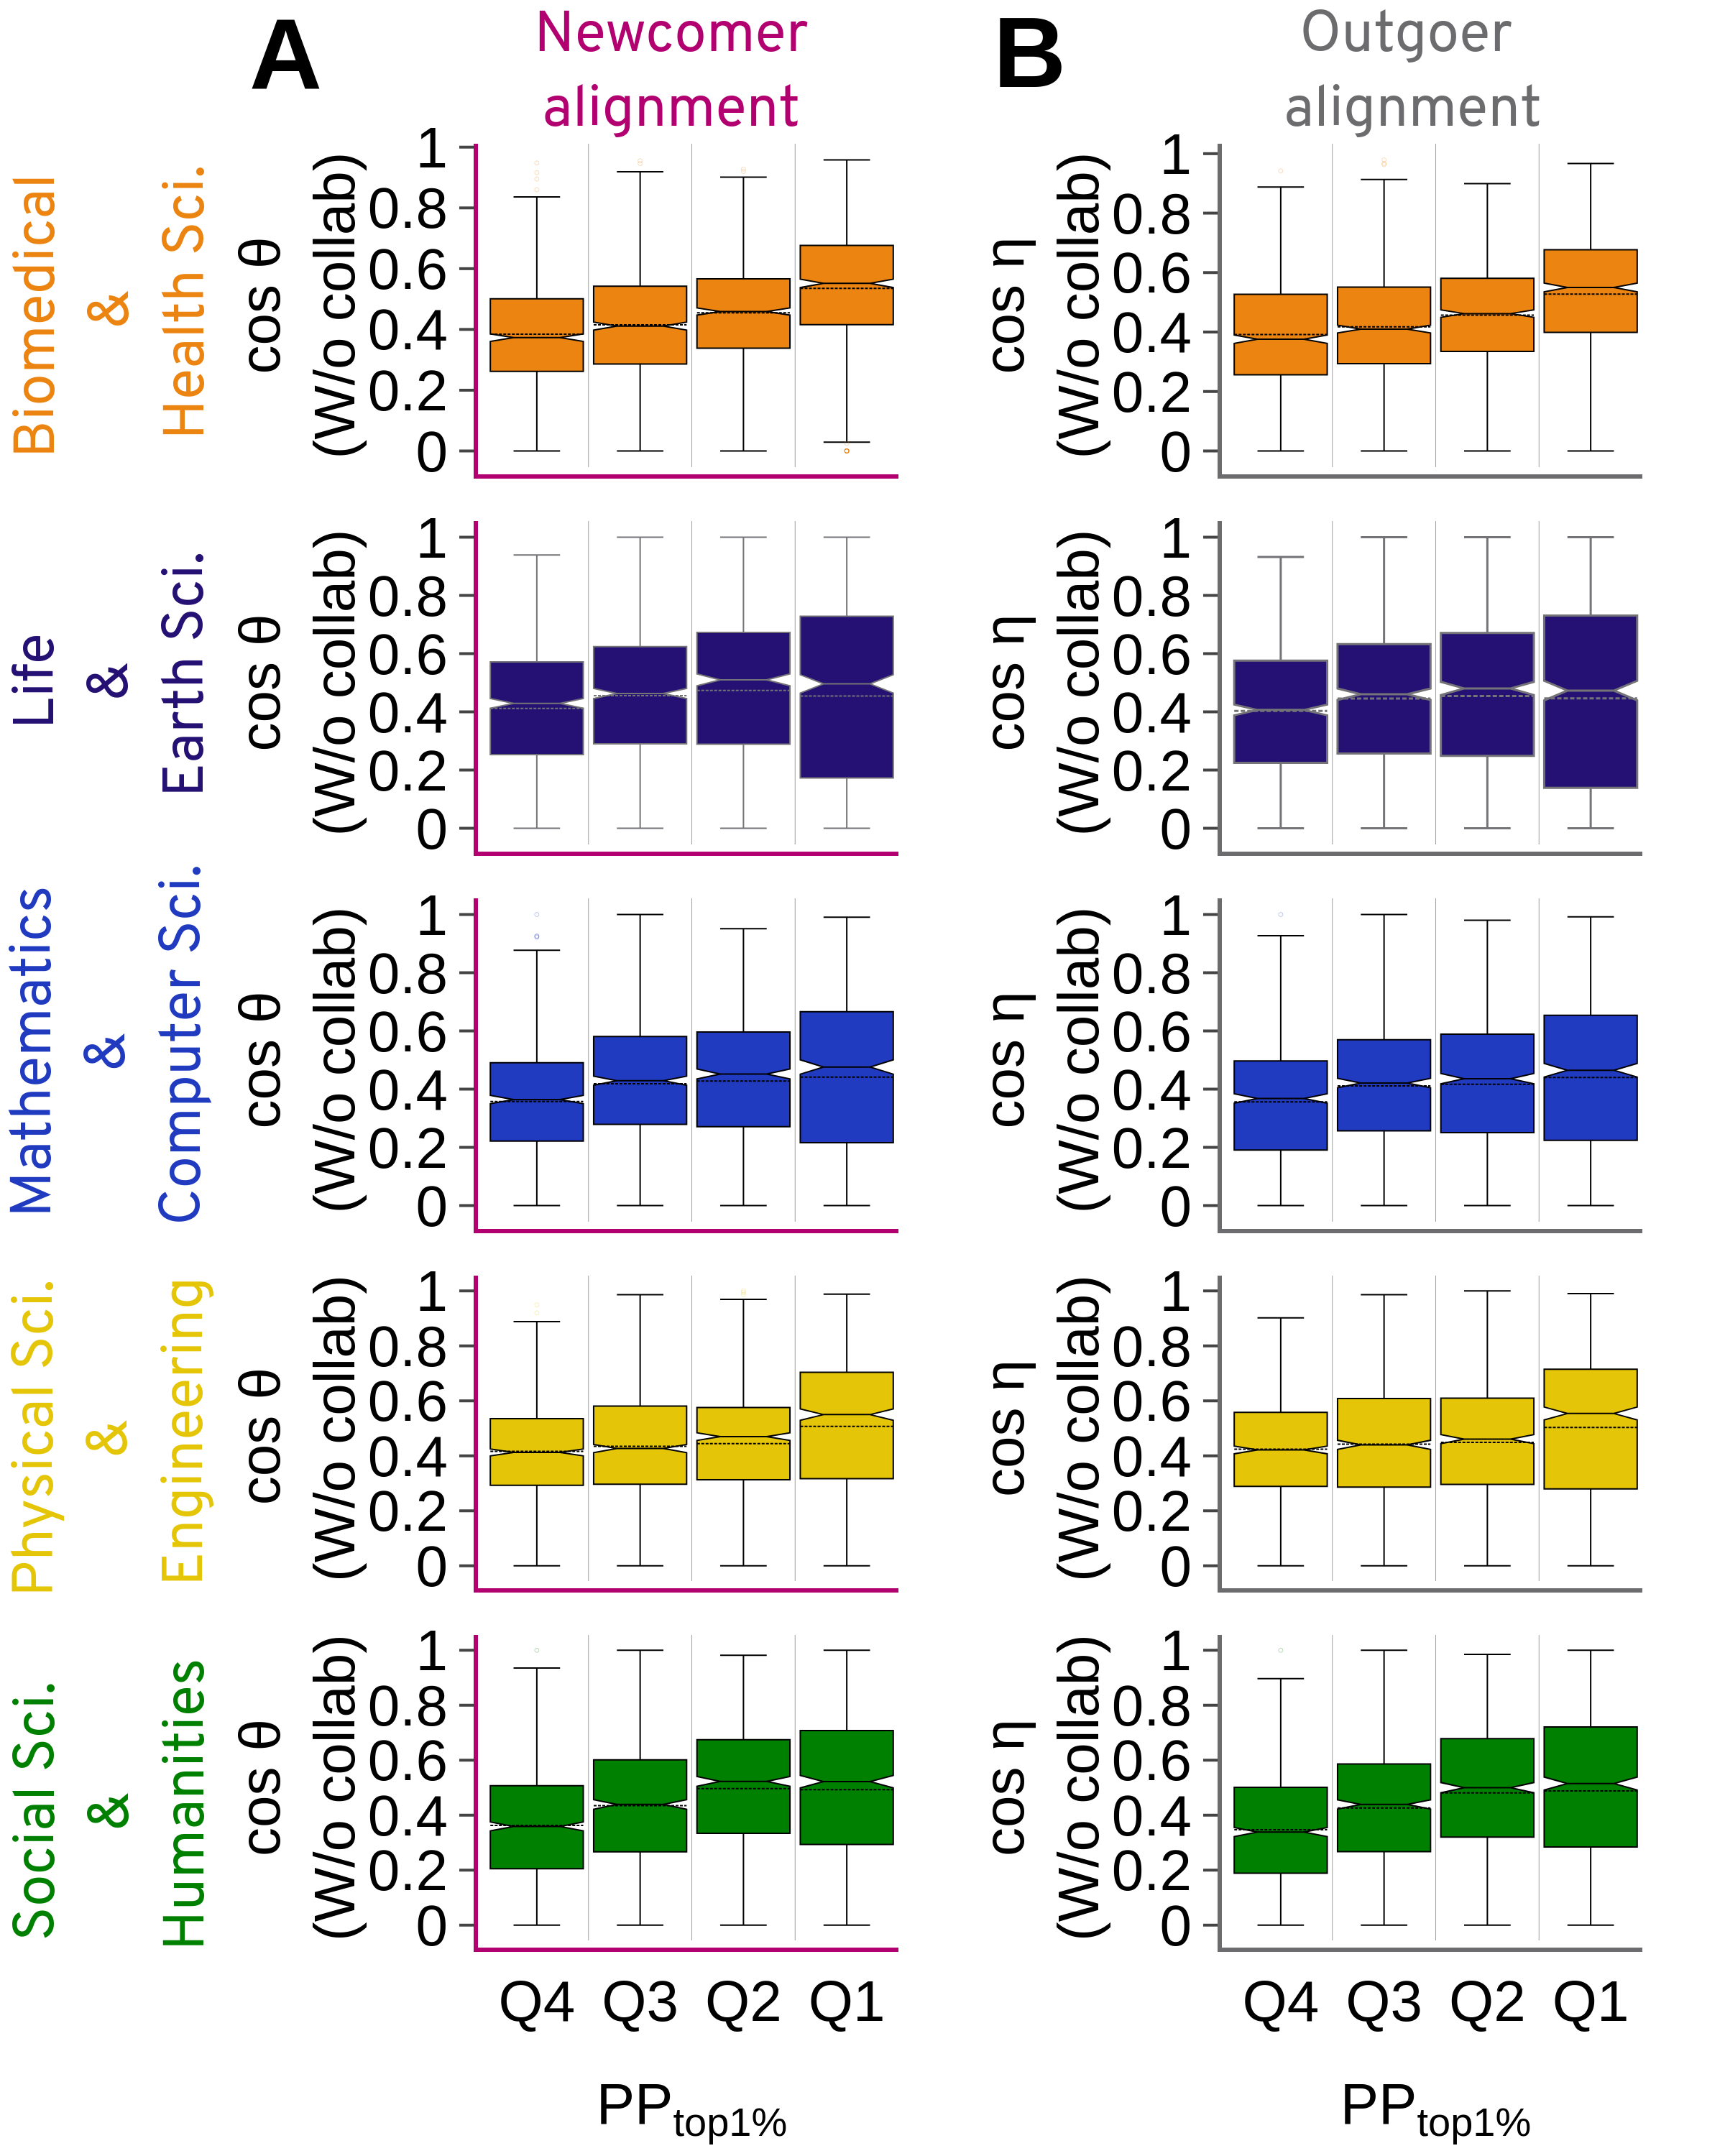
\includegraphics[width=0.5\linewidth]{figures_alignment/figure8ab.png}
\caption{Boxplots of newcomer skill alignment, $\cos{\theta}$(W/o collab), and outgoer skill alignment, $\cos{\eta}$(W/o collab), by major fields of science and quartiles of PP$_{top1\%}$. We provide an overview of disciplinary trends in the alignment of mobile researchers' skills that occurs when scholars within an institution do not collaborate.
Top-cited institutions have higher alignment than average organizations (two-sample $t$ test, $P$ value <0.001) even when researchers do not collaborate internally. This finding can be generalized across large scientific fields and suggests that the alignment of capabilities that occurs from non-collaborative work positively affects the citation visibility of institutions. Here the quartiles from low impact (i.e., quartile 4) to high impact (i.e., quartile 1) and the disciplines are arranged alphabetically from top to bottom. The panels have the same setting as the Figure~\ref{fig4:figure4ab.png}, but this time for the $\cos\theta$ (W/o collab) and $\cos\eta$ (W/o collab) measures, i.e., for the case of non-collaborative hires and leavers. We find that the alignment of their skills is significantly lower across impact quartiles and disciplines. Nevertheless, alignment scores are higher for the most cited institutions (i.e., quartile 1) than for the least cited institutions (i.e., quartile 4). This tells us that internal collaboration is also an important factor in integrating knowledge and aligning skills in institutions and across the disciplines in which the institutions operate. Moreover, the most frequently cited institutions still attract and nurture similarly skilled researchers, even if they do not collaborate on scientific publications within the institution. 
}
\label{SI:figure8ab.png}
\end{figure}

\subsection{Classification of disambiguated authors into Newcomers, Natives, and Outgoers~\label{SI2}}
Researchers affiliated with each organization in the data are split into three categories based on where they began publishing in relation to the organization being analyzed: a) Natives -- are those who started publishing on the same organization and have not (yet) changed their affiliation, b) Newcomers -- are those who started publishing on a different organization, and c) Outgoers -- are those who left the first organization where they published at some point under the period of analysis (2000-2020). 

\subsection{Multivariate Linear Regression Analysis~\label{SI4}} 
In this section, we delve into the details of our regression analysis. We first define several indicators to better understand the connection between skill alignment, intra-institutional collaboration, scientific impact, and productivity measures. To ensure the validity of our findings, we also conduct robustness checks to test whether our main findings still hold when alternative measures of scientific influence are used (see sections~\hyperref[SI4.1]{SI Text 2.1}, and ~\hyperref[SI4.2]{SI Text 2.2}).

%%%%%%%%%%%%%%%%%%%%%%%%%%%%%%%%%%%%%%%%
%%%%%%%%%%          NEWCOMER REGRESSOR             %%%%%%%%%%
%%%%%%%%%%%%%%%%%%%%%%%%%%%%%%%%%%%%%%%%
\subsubsection{Regression of newcomer skill alignment~\label{SI4.1}}
Our main results are based on a multivariate linear ordinary least squares regression model as below:

\begin{equation} \label{equation 7}
\begin{array}{lcl}
{\cos \theta}_{i} &=& \beta_0\\
%&& + \beta_{1} {\mathrm{PP}_{\mathrm{top\,nth\%}_{i}}}\\
&& + \beta_{1,2} {\mathrm{X}}_{i}\\
&& + \beta_{3} {\mathrm{r}}_{i}\\
&& + \beta_{4} {\mathrm{PP}_{\nu}}_{i}\\
&& + \beta_{5} {\mathrm{PPP}\,(\mathrm{collab}_{\nu})_{i}}\\
&& + \beta_{6} {\mathrm{PPS}_{i}: \mathrm{Diversified}}\\
&& + \epsilon_i \, .\\
\end{array}
\end{equation} 

\textbf{Dependent Variable.} The dependent variable  is a measure of how closely the skills of newcomers and the existing workforce at an institution, $i$, match. This measure is represented by $\cos{\theta}_i$ ,which is defined in~\hyperref[Definition of skills section]{Eq.~1}.  Additionally, we also use another measure, $\cos{\eta}_i$, for outgoers who have changed their institutional affiliations, which is defined in ~\hyperref[Definition of skills section]{Eq.~2}.  

\textbf{Predictors of Interest.}The predictors of interest in this study are three percentile-based citation impact metrics (PP$_\mathrm{top,1\%i}$, PP$\mathrm{top,5\%i}$, and PP$\mathrm{top,10\%_i}$) and a continuous variable of normalized citation counts (TNCS$_i$). These measures will be used to explain the skill alignment of newcomers and existing workforce in an institution by using a regression model. For the term X$_i$ in Eq.~\ref{equation 7} we first use three percentile-based independent variables, PP$_\mathrm{top\,1\%_i}$, PP$_\mathrm{top\,5\%_i}$, and PP$_\mathrm{top\,10\%_i}$, which indicate the fractions of upper-tail papers being the top 1\%, 5\%, and 10\%, respectively, as measured by citation (see definition in ~\hyperref[Definition of skills section]{Eq.~6}). These measures are included separately in different regression models, with coefficient $\beta_1$. Finally, with coefficient $\beta_2$, we use an alternative measure of scientific impact in X$_i$, the continuous variable TNCS$_{i}$, defined in \hyperref[Definition of skills section]{Eq.~5}, which measures the total normalised citation count of a scientific institution.

\textbf{Control Variables.} In this study, several other explanatory variables are included as independent variables to control for other possible predictors of workforce skill alignment. These variables include size and internal collaboration indicators at the institutional level. Descriptive statistics on the variables used in the regression analysis are presented in \hyperref[Table S1]{Table S1}. The following control variables will be used in the regression analysis of newcomers' skill alignment presented in this section:

\newcommand\textequal{%
 \rule[.4ex]{4pt}{0.4pt}\llap{\rule[.7ex]{4pt}{0.4pt}}}

\begin{itemize} 
  \item r$_{i}$~\textequal~indicates the total number of researchers at a research institution 
  \item PP$_{\nu_i}$~\textequal~ indicates the proportion of newcomers of a research institution
  \item PPP (collab$_\nu)_{i}$~\textequal~indicates the proportion of publications in collaboration between newcomers and the rest of the institution
 \item PPS$_{i}$~\textequal~ is a dichotomous variable that indicates whether an institution has an overall diversified or specialized skills' portfolio. It indicates the absence or presence of diversification or specialization that may be expected to shift the outcome of skill alignment produced by the total workforce of a research institution. PPS$_{i}$ = 1 if the institution has produced an above median proportion of skills and PPS$_{i}$ = 0 otherwise
\end{itemize}

These control variables are used to account for other factors that may influence the skill alignment of newcomers and existing workforce in an institution. Furthermore, we included PPS$_{i}$, and r$_{i}$ in all regression models. All independent variables included in the regression models had a variance inflation score (VIF) well below four, below the tolerance threshold of 0.25. 

\textbf{Stratification by Size of Institutions.} The total publication output, $P_{i}$, is used as an indicator of the size of an institution. Institutions' size has been shown to affect the ability of institutions to attract researchers \cite{machavcek2022researchers, clauset2015systematic, Zhang22}. It is therefore assumed that size also modifies the proportion of publications in the top $1\%$, $5\%$, and $10\%$ of an institution's publications on skill alignment. To control for this confounding effect, we stratified institutions into three subgroups based on their publication production, creating subgroups in which an institution's publication production varies less than all institutions in the sample combined. This stratification strategy will be applied in all regression models.

The main results of the stratified regression analysis are presented in ~\hyperref[Table S2]{Table S2},~\hyperref[Table S3]{Table S3}, and ~\hyperref[Table S4]{Table S4}. The coefficients of the tables are standardized. Standardizing the coefficients allows us to compare the strength of the effect of each individual independent variable on the dependent variable. This is important because size-dependent associations can produce substantially higher correlation coefficients, especially when they exhibit substantial variance \cite{traag2019systematic}. This can potentially alter the relative associations between alignment and normalized count-based citation measures. 

The results of models (1), (2), (3), and (4) in the three tables suggest that there is a significant relationship between an institution's skill alignment and the proportion of publications in the top 1\%, 5\%, 10\%, and Total Normalized Citation Score (TNCS) after controlling for several other explanatory variables. These variables include the proportion of incoming researchers, the proportion of internal collaboration between the newcomers and the rest of the institution's workforce, the total workforce, and the degree of diversification of skills. This relationship is consistent across all subgroups of institutional size. The findings also indicate that skill alignment is, on average, lower in diversified institutions than in specialized institutions, as indicated by the binary variable PPS$_{i}$: Diversification/Specialization, which was negative in all models and tables. In specialized institutions, which are more thematically focused, the expertise of mobile researchers better matches the expertise of their institutions, while in diversified institutions there are more opportunities for topical diversification. The proportion of incoming researchers, while significant, does not appear to be a particularly strong predictor of skill alignment.

Collaboration activity within the institution is one of the strongest predictors of skill alignment, with a standardized coefficient between 0.455 and 0.442 across different subgroups of institutional size. This suggests that institutions that encourage internal collaboration among researchers may be more successful in aligning the expertise of newcomers with that of the institution as a whole. The proportion of papers in the top 1\%, 5\% and 10\% of highly cited publications are also found to be significantly associated with skill alignment, with standardized coefficients of 0.168(0.026), 0.214(0.028) and 0.203(0.028) respectively in, for example,~\hyperref[Table S2]{Table S2}. For medium and high output institutions, total workforce capacity (r$_{i}$) is also found to be considerably associated with higher levels of alignment, with the coefficients ranging from 0.224(0.023) to 0.213(0.024) in~\hyperref[Table S3]{Table S3} and slightly higher for high output institutions, ranging from 0.307(0.048) to 0.288(0.022) in~\hyperref[Table S4]{Table S4}.

Overall, these results suggest that internal collaboration and citation impact likely explain the alignment at institutions, particularly in institutions with lower publication output, while medium and large publication output institutions also achieve greater alignment by attracting most of the available scientific labour~\cite{Zhang22}. The citation impact variables for medium and large institutions remain significantly associated with alignment, except for the total normalized citation score (TNCS$_{i}$) in model (4) in ~\hyperref[Table S4]{Table S4} for high output institutions. This suggests that while publications at the high end of the citation percentile scale may play a role in aligning an institutions expertise, citation `quantity' does not have a direct effect on the alignment of skills among newcomers and the rest of the workforce in larger scientific institutions. 

%%%%%%%%%%%%%%%%%%%%%%%%%%%%%%%%%%%%%%%%%%
%%%%%% Overall descriptive statistics %%%%
%%%%%%%%%%%%%%%%%%%%%%%%%%%%%%%%%%%%%%%%%%

\begin{table}[!ht]
\caption{Descriptive statistics of the main indicators and control variables for all academic institutions in the sample (mean, median, standard deviation, skewness, and kurtosis).}
\label{Table S1}
\centering
\begin{tabular}{@{}
>{\columncolor[HTML]{FFFFFF}}c 
>{\columncolor[HTML]{FFFFFF}}c 
>{\columncolor[HTML]{FFFFFF}}c 
>{\columncolor[HTML]{FFFFFF}}c 
>{\columncolor[HTML]{FFFFFF}}l 
>{\columncolor[HTML]{FFFFFF}}l 
>{\columncolor[HTML]{FFFFFF}}l @{}}
\toprule
\multicolumn{7}{c}{\cellcolor[HTML]{FFFFFF}\textbf{Descriptive Statistics}}         \\ \midrule
N                          & N   & Mean & Median & \multicolumn{1}{c}{\cellcolor[HTML]{FFFFFF}Std. Deviation} & Skewness & Kurtosis \\ \midrule
PP$_{top1\%_i}$   & 3,965 & 0.02   & 0.01   & 0.01   & 2.25 & 11.58 \\ \midrule
PP$_{top5\%_i}$ & 3,965 & 0.07   & 0.06   & 0.03   & 1.35 & 3.77 \\ \midrule
PP$_{top10\%_i}$ & 3,965 & 0.13   & 0.12   & 0.05   & 0.97 & 1.69 \\ \midrule
TNCS$_{i}$  & 3,965 & 9,809.58 & 3,813.59 & 18,324.12 & 5.36 & 41.00 \\ \midrule
P$_{i}$      & 3,965 & 7,196.51 & 3,610.00 & 11,238.25 & 4.27 & 24.13 \\ \midrule
r$_{i}$    & 3,965 & 3,834.33 & 1,894.00 & 5,899.69 & 4.99 & 40.13 \\ \midrule
PP$_{\nu_i}$    & 3,965 & 0.41   & 0.39   & 0.17   & 0.37 & -0.55 \\ \midrule
PP$_{\omega_i}$      & 3,965 & 0.19   & 0.19   & 0.06   & 0.46 & 0.58 \\ \midrule
PPP (collab$_{\nu})_{i}$ & 3,965 & 0.30   & 0.30   & 0.10   & 0.40 & 1.68 \\ \midrule
PPP (collab$_{\omega})_{i}$ & 3,965 & 0.27  & 0.27   & 0.11   & 0.44 & 0.60 \\ \midrule
PPS$_{i}$  & 3,965 & 0.21  & 0.17 & 0.13 & 1.15 & 0.87 \\ \midrule
cos $\theta_i$        & 3,965 & 0.82 & 0.84  & 0.10                            & -0.99  & 1.41   \\ \midrule
cos $\eta_i$       & 3,965 & 0.84 & 0.86  & 0.10                            & -1.24  & 2.16   \\ \midrule
cos $\theta$ (W/o collab)$_{i}$ & 3,965 & 0.55 & 0.54  & 0.17                            & 0.19   & -0.45  \\ \midrule
cos $\eta$ (W/o collab)$_{i}$  & 3,965 & 0.60 & 0.61  & 0.17                            & -0.16  & -0.52  \\ \bottomrule
\end{tabular}
\end{table}

%%%%%%%%%%%%%%%%%%%%%%%%%%%%%%%%%%%
% Models for Low Output Universities
%%%%%%%%%%%%%%%%%%%%%%%%%%%%%%%%%%%
% Date and time: Mon, Dec 19, 2022 - 11:12:12
\begin{table}[!htbp] \centering 
  \caption{Relationship between low output institutions' citation impact and newcomer skill alignment. To allow comparison of the coefficients in the table, all variables were centred. Therefore, the beta coefficients in the table have standard deviations as their units. The results in models (1), (2), (3), and (4) show that the proportion of publications in the top 1\%, 5\%, 10\% and the continuous variable TNCS$_{i}$ have a significant association with the alignment between newcomers and the rest of the workforce. The degree of internal collaboration within institution, PPP(collab$_{\nu})_{i}$, is found to be most strongly associated with alignment, while the proportion of newcomers, PP$_{\nu_i}$, and the total workforce, r$_{i}$, are least strongly associated with skill alignment.}
  \label{Table S2} 
\small 
\scriptsize
\begin{tabularx}{\textwidth}{@{\extracolsep{\fill}}lcccc}
\\[-1.8ex]\hline 
\hline \\[-1.8ex] 
 & \multicolumn{3}{c}{\textit{Dependent variable: $\cos{\theta}_{i}$}} \\ 
\cline{2-5} 
\\[-1.8ex] & \multicolumn{4}{c}{Institutions with Low Publication Output, P$_{i}$ [387, 2425]} \\ 
\\[-1.8ex] & (1) & (2) & (3) & (4)\\ 
\hline \\[-1.8ex] 
 Constant & 0.086$^{***}$ (0.025) & 0.082$^{***}$ (0.025) & 0.080$^{***}$ (0.025) & 0.093$^{***}$ (0.025) \\ 
  r$_{i}$ & 0.094$^{***}$ (0.023) & 0.096$^{***}$ (0.023) & 0.098$^{***}$ (0.023) & 0.088$^{***}$ (0.023) \\ 
  PP$_{\nu_i}$ & 0.137$^{***}$ (0.025) & 0.106$^{***}$ (0.027) & 0.094$^{***}$ (0.028) & 0.143$^{***}$ (0.025) \\ 
  PPP (collab$_\nu)_{i}$ & 0.455$^{***}$ (0.022) & 0.446$^{***}$ (0.022) & 0.442$^{***}$ (0.022) & 0.443$^{***}$ (0.023) \\ 
  PP$_{{top\,1\%}_{i}}$ & 0.168$^{***}$ (0.026) &  &  &  \\ 
  PP$_{{top\,5\%}_{i}}$ &  & 0.203$^{***}$ (0.028) &  &  \\ 
  PP$_{{top\,10\%}_{i}}$ &  &  & 0.214$^{***}$ (0.028) &  \\ 
  TNCS$_{i}$ &  &  &  & 0.164$^{***}$ (0.025) \\ 
 \hline \\[-1.8ex] 
PPS$_{i}$: Diversification dummy? & Yes & Yes & Yes & Yes \\ 
\hline \\[-1.8ex] 
Observations & 1,322 & 1,322 & 1,322 & 1,322 \\ 
Adjusted R$^{2}$ & 0.386 & 0.391 & 0.392 & 0.385 \\ 
Residual Std. Error (df = 1316) & 0.784 & 0.780 & 0.780 & 0.784 \\ 
F Statistic (df = 5; 1316) & 166.946$^{***}$ & 170.617$^{***}$ & 171.361$^{***}$ & 166.655$^{***}$ \\ 
\hline 
\hline \\[-1.8ex] 
Standard errors in parentheses. & \multicolumn{4}{l}{$^{*}$p$<$0.1; $^{**}$p$<$0.05; $^{***}$p$<$0.01} \\ 
\end{tabularx}
\end{table} 


%%%%%%%%%%%%%%%%%%%%%%%%%%%%%%%%%%%%%%%
% Models for Medium Output Universities
%%%%%%%%%%%%%%%%%%%%%%%%%%%%%%%%%%%%%%%
% Date and time: Mon, Dec 19, 2022 - 11:34:21
\begin{table}[!htbp] \centering 
  \caption{Relationship between medium output institutions' citation impact and newcomer skill alignment. To allow comparison of the coefficients in the table, all variables were centred. Therefore, the beta coefficients in the table have standard deviations as their units. The results in models (1), (2), (3), and (4) show that the proportion of publications in the top 1\%, 5\%, 10\% and the continuous variable TNCS$_{i}$ have a significant association with the alignment between newcomers and the rest of the workforce. The degree of internal collaboration within institution, PPP(collab$_{\nu})_{i}$, is most strongly associated with alignment within institutions, followed by the total workforce, r$_{i}$, of the institution while the proportion of newcomers, PP$_{\nu_i}$ is least strongly associated with skill alignment.} 
  \label{Table S3} 
\small 
\scriptsize
\begin{tabularx}{\textwidth}{@{\extracolsep{\fill}}lcccc}
\hline \\[-1.8ex] 
 & \multicolumn{4}{c}{\textit{Dependent variable: $\cos{\theta}_{i}$}} \\ 
\cline{2-5} 
\\[-1.8ex] & \multicolumn{4}{c}{Institutions with Medium Publication Output, P$_{i}$ [2425, 4864]} \\ 
\\[-1.8ex] & (1) & (2) & (3) & (4)\\ 
\hline \\[-1.8ex] 
 Constant & 0.244$^{***}$ (0.031) & 0.248$^{***}$ (0.031) & 0.249$^{***}$ (0.031) & 0.257$^{***}$ (0.031) \\ 
  r$_{i}$ & 0.224$^{***}$ (0.023) & 0.222$^{***}$ (0.023) & 0.222$^{***}$ (0.023) & 0.213$^{***}$ (0.024) \\ 
  PP$_{\nu_i}$ & 0.073$^{***}$ (0.024) & 0.062$^{**}$ (0.024) & 0.059$^{**}$ (0.024) & 0.096$^{***}$ (0.024) \\ 
  PPP (collab$_\nu)_{i}$ & 0.431$^{***}$ (0.022) & 0.426$^{***}$ (0.022) & 0.423$^{***}$ (0.022) & 0.429$^{***}$ (0.022) \\ 
  PP$_{{top\,1\%}_{i}}$ & 0.182$^{***}$ (0.024) &  &  &  \\ 
  PP$_{{top\,5\%}_{i}}$ &  & 0.202$^{***}$ (0.024) &  &  \\ 
  PP$_{{top\,10\%}_{i}}$ &  &  & 0.208$^{***}$ (0.024) &  \\ 
  TNCS$_{i}$ &  &  &  & 0.140$^{***}$ (0.024) \\ 
 \hline \\[-1.8ex] 
PPS$_{i}$: Diversification dummy? & Yes & Yes & Yes & Yes \\ 
\hline \\[-1.8ex] 
Observations & 1,321 & 1,321 & 1,321 & 1,321 \\ 
Adjusted R$^{2}$ & 0.406 & 0.412 & 0.414 & 0.396 \\ 
Residual Std. Error (df = 1315) & 0.770 & 0.767 & 0.766 & 0.777 \\ 
F Statistic (df = 5; 1315) & 181.735$^{***}$ & 186.102$^{***}$ & 187.440$^{***}$ & 174.110$^{***}$ \\ 
\hline 
\hline \\[-1.8ex] 
Standard errors in parentheses. & \multicolumn{4}{l}{$^{*}$p$<$0.1; $^{**}$p$<$0.05; $^{***}$p$<$0.01} \\ 
\end{tabularx} 
\end{table} 

%%%%%%%%%%%%%%%%%%%%%%%%%%%%%%%%%%%%%%%
% Models for High Output Universities
%%%%%%%%%%%%%%%%%%%%%%%%%%%%%%%%%%%%%%%
% Date and time: Mon, Dec 19, 2022 - 12:01:16
\begin{table}[!htbp] \centering 
  \caption{Relationship between high output institutions' citation impact and newcomer skill alignment. To allow comparison of the coefficients in the table, all variables were centred. Therefore, the beta coefficients in the table have standard deviations as their units. The results in models (1), (2), (3), and (4) show that the proportion of publications in the top 1\%, 5\%, 10\% have a significant association with the alignment between newcomers and the rest of the workforce. The degree of internal collaboration within institution, PPP(collab$_{\nu})_{i}$, is most strongly associated with alignment within institutions, followed by the total workforce, r$_{i}$, of the institution while the proportion of newcomers, PP$_{\nu_i}$ is least strongly associated with skill alignment.} 
  \label{Table S4} 
\small 
\scriptsize
\begin{tabularx}{\textwidth}{@{\extracolsep{\fill}}lcccc}
\\[-1.8ex]\hline 
\hline \\[-1.8ex] 
 & \multicolumn{4}{c}{\textit{Dependent variable: $\cos{\theta}_{i}$}} \\ 
\cline{2-5} 
\\[-1.8ex] & \multicolumn{4}{c}{Institutions with High Publication Output, P$_{i}$ [4864, 121750]} \\ 
\\[-1.8ex] & (1) & (2) & (3) & (4)\\ 
\hline \\[-1.8ex] 
 Constant & 0.588$^{***}$ (0.086) & 0.584$^{***}$ (0.086) & 0.588$^{***}$ (0.086) & 0.693$^{***}$ (0.085) \\ 
  r$_{i}$ & 0.295$^{***}$ (0.022) & 0.288$^{***}$ (0.022) & 0.288$^{***}$ (0.022) & 0.307$^{***}$ (0.048) \\ 
  PP$_{\nu_i}$ & 0.070$^{***}$ (0.027) & 0.057$^{**}$ (0.027) & 0.058$^{**}$ (0.027) & 0.162$^{***}$ (0.022) \\ 
  PPP (collab$_\nu)_{i}$ & 0.429$^{***}$ (0.021) & 0.425$^{***}$ (0.021) & 0.422$^{***}$ (0.021) & 0.424$^{***}$ (0.022) \\ 
  PP$_{{top\,1\%}_{i}}$ & 0.159$^{***}$ (0.028) &  &  &  \\ 
  PP$_{{top\,5\%}_{i}}$ &  & 0.178$^{***}$ (0.029) &  &  \\ 
  PP$_{{top\,10\%}_{i}}$ &  &  & 0.175$^{***}$ (0.029) &  \\ 
  TNCS$_{i}$ &  &  &  & 0.021 (0.048) \\ 
 \hline \\[-1.8ex] 
PPS$_{i}$: Diversification dummy?  & Yes & Yes & Yes & Yes \\ 
\hline \\[-1.8ex] 
Observations & 1,322 & 1,322 & 1,322 & 1,322 \\ 
Adjusted R$^{2}$ & 0.430 & 0.432 & 0.432 & 0.416 \\ 
Residual Std. Error (df = 1316) & 0.755 & 0.754 & 0.754 & 0.764 \\ 
F Statistic (df = 5; 1316) & 199.974$^{***}$ & 202.121$^{***}$ & 201.545$^{***}$ & 188.853$^{***}$ \\ 
\hline 
\hline \\[-1.8ex] 
Standard errors in parentheses. & \multicolumn{4}{l}{$^{*}$p$<$0.1; $^{**}$p$<$0.05; $^{***}$p$<$0.01} \\ 
\end{tabularx} 
\end{table} 

%%%%%%%%%%%%%%%%%%%%%%%%%%%%%%%%%%%%%%%%
%%%%%%%%%% OUTGOER  REGRESSOR %%%%%%%%%% 
%%%%%%%%%%%%%%%%%%%%%%%%%%%%%%%%%%%%%%%%
\subsubsection{Regression of outgoer skill alignment ~\label{SI4.2}}
The results in this section are based on a multivariate linear ordinary least squares regression model as below:

\begin{equation} \label{equation 9}
\begin{array}{lcl}
{\cos \eta}_{i} &=& \beta_0\\
%&&+  \beta_{1} {\mathrm{PP}_{\mathrm{top\,nth\%}_{i}}}\\
&& + \beta_{1,2} {\mathrm{X}}_{i}\\
&& + \beta_{3} {\mathrm{r}}_{i}\\
&& + \beta_{4} {\mathrm{PP}_{\omega}}_{i}\\
&& + \beta_{5} {\mathrm{PPP}\,(\mathrm{collab}_{\omega})_{i}}\\
&& + \beta_{6} {\mathrm{PPS}_{i}: \mathrm{Diversified}}\\
&& + \epsilon_i \, .\\
\end{array}
\end{equation} 

\textbf{Dependent Variable.} The dependent variable is the skill alignment of the outgoer and remaining workforce of an institution, $i$, $\cos{\eta}_i$ defined in~\hyperref[Definition of skills section]{Eq.~2}. 

\textbf{Predictors of Interest.} Just like in the previous section, we use, for the term X$_i$, three percentile-based independent variables, ${ PP }_{top1\%}$, ${ PP }_{top5\%}$, and ${ PP }_{top10\%}$, measures to indicate the fractions of upper-tail papers being the top 1\%, 5\%, and 10\%, respectively, gauged by citation (See definition in the~\hyperref[Definition of skills section]{Eq.~6}). These measures are included separately in different regression models with coefficient $\beta_1$. The total normalized citation counts of a scientific institution TNCS$_i$, defined in ~\hyperref[Definition of skills section]{Eq.~5} is also tested in X$_i$ with coefficient $\beta_2$.

\textbf{Control Variables.} In order to account for other potential factors that may impact outgoer skill alignment, we have included a number of explanatory variables in our analysis. These variables include measures of institutional size and internal collaboration, and the descriptive statistics for these variables can be found in~\hyperref[Table S1]{Table S1}. These variables will be used as control variables in our regression analysis.

\begin{itemize} 
  \item r$_{i}$~\textequal~indicates the total number of researchers at a research institution 
  \item PP$\omega_{i}$~\textequal~ indicates the proportion of outgoers of a research institution
  \item PPP (collab$_{\omega})_{i}$~\textequal~indicates the proportion of publications in collaboration between outgoers and natives of the institution
  \item PPS$_{i}$~\textequal~ is a dichotomous variable that indicates whether an institution has an overall diversified or specialized skills' portfolio. It indicates the absence or presence of diversification or specialization that may be expected to shift the outcome of skill alignment produced by the total workforce of a research institution. PPS = 1 if the institution has produced an above median proportion of skills and PPS = 0 otherwise 
\end{itemize}

These control variables are used to account for other factors that may influence the skill alignment of outgoers and existing workforce in an institution. Furthermore, we included PPS$_{i}$, and r$_{i}$ in all regression models. All independent variables included in the regression models had a variance inflation score (VIF) well under four, below the tolerance threshold of 0.25.

\textbf{Stratification by Size of Institutions.} The total publication output, $P_{i}$, is used as an indicator of the size of an institution. Institutions' size has been shown to affect the ability of institutions to attract researchers \cite{machavcek2022researchers, clauset2015systematic}. It is therefore assumed that size also modifies the proportion of publications in the top $1\%$, $5\%$, and $10\%$ of an institution's publications on outgoer skill alignment. Stratification allows us to control for this confounding effect by creating three subgroups in which an institution's publication production varies less than all institutions in our sample combined.

%%%%%%%%%%%%%%%%%%%%%%%%%%%%%%%%%%%%%%%
% Models for Low Output Universities
%%%%%%%%%%%%%%%%%%%%%%%%%%%%%%%%%%%%%%%
% Date and time: Mon, Dec 19, 2022 - 12:41:21
\begin{table}[!htbp] \centering 
  \caption{Relationship between low output institutions' citation impact and outgoer skill alignment. To allow comparison of the coefficients in the table, all variables were centred. Therefore, the beta coefficients in the table have standard deviations as their units. The results in models (1), (2), (3), and (4) show that the proportion of publications in the top 1\%, 5\%, 10\% and the continuous variable TNCS$_{i}$ have a significant association with the alignment between outgoers and the rest of the workforce. The degree of internal collaboration within institution, PPP(collab$_{\omega})_{i}$, is most strongly associated with alignment within institutions, followed by the total workforce, r$_{i}$ of the institution while the proportion of newcomers, PP$_{\omega_i}$ and the total workforce, r$_{i}$, are least strongly associated with skill alignment.} 
  \label{Table S5} 
  \label{} 
\small 
\scriptsize
\begin{tabularx}{\textwidth}{@{\extracolsep{\fill}}lcccc}
\\[-1.8ex]\hline 
\hline \\[-1.8ex] 
 & \multicolumn{4}{c}{\textit{Dependent variable: $\cos{\eta}_{i}$}} \\ 
\cline{2-5} \\[-1.8ex] & \multicolumn{4}{c}{Institutions with Low Publication Output, P$_{i}$ [387, 2425]} \\ 
\\[-1.8ex] & (1) & (2) & (3) & (4)\\ 
\hline \\[-1.8ex] 
 Constant & 0.084$^{***}$ (0.023) & 0.077$^{***}$ (0.022) & 0.074$^{***}$ (0.022) & 0.094$^{***}$ (0.023) \\ 
  r$_{i}$ & 0.118$^{***}$ (0.022) & 0.114$^{***}$ (0.021) & 0.115$^{***}$ (0.021) & 0.113$^{***}$ (0.022) \\ 
  PP$_{\omega_i}$ & 0.166$^{***}$ (0.025) & 0.163$^{***}$ (0.024) & 0.160$^{***}$ (0.024) & 0.161$^{***}$ (0.025) \\ 
  PPP (collab$_\omega)_{i}$ & 0.471$^{***}$ (0.025) & 0.476$^{***}$ (0.025) & 0.478$^{***}$ (0.025) & 0.459$^{***}$ (0.025) \\ 
  PP$_{{top\,1\%}_{i}}$ & 0.212$^{***}$ (0.020) &  &  &  \\ 
  PP$_{{top\,5\%}_{i}}$ &  & 0.236$^{***}$ (0.020) &  &  \\ 
  PP$_{{top\,10\%}_{i}}$ &  &  & 0.243$^{***}$ (0.020) &  \\ 
  TNCS$_{i}$ &  &  &  & 0.205$^{***}$ (0.020) \\ 
 \hline \\[-1.8ex] 
PPS$_{i}$: Diversification dummy? & Yes & Yes & Yes & Yes \\ 
\hline \\[-1.8ex] 
Observations & 1,322 & 1,322 & 1,322 & 1,322 \\ 
Adjusted R$^{2}$ & 0.484 & 0.493 & 0.496 & 0.482 \\ 
Residual Std. Error (df = 1316) & 0.718 & 0.712 & 0.710 & 0.720 \\ 
F Statistic (df = 5; 1316) & 248.656$^{***}$ & 258.183$^{***}$ & 260.884$^{***}$ & 246.584$^{***}$ \\ 
\hline 
\hline \\[-1.8ex] 
Standard errors in parentheses. & \multicolumn{4}{l}{$^{*}$p$<$0.1; $^{**}$p$<$0.05; $^{***}$p$<$0.01} \\ 
\end{tabularx} 
\end{table} 

%%%%%%%%%%%%%%%%%%%%%%%%%%%%%%%%%%%%%%%
% Models for Medium Output Universities
%%%%%%%%%%%%%%%%%%%%%%%%%%%%%%%%%%%%%%%
% Date and time: Mon, Dec 19, 2022 - 12:48:09
\begin{table} \centering 
  \caption{Relationship between high output institutions' citation impact and outgoer skill alignment. To allow comparison of the coefficients in the table, all variables were centred. Therefore, the beta coefficients in the table have standard deviations as their units. The results in models (1), (2), (3), and (4) show that the proportion of publications in the top 1\%, 5\%, 10\% have a significant association with the alignment between outgoers and the rest of the workforce. The degree of internal collaboration within institution, PPP(collab$_{\omega})_{i}$, is most strongly associated with alignment within institutions, followed by the total workforce, r$_{i}$, of the institution while the proportion of outgoers, PP$_{\omega_i}$, is least strongly associated with skill alignment.} 
  \label{Table S6} 
\small 
\scriptsize
\begin{tabularx}{\textwidth}{@{\extracolsep{\fill}}lcccc}
\\[-1.8ex]\hline 
\hline \\[-1.8ex] 
 & \multicolumn{4}{c}{\textit{Dependent variable: $\cos{\eta}_{i}$}} \\ 
\cline{2-5} 
\\[-1.8ex] & \multicolumn{4}{c}{Institutions with Medium Publication Output, P$_{i}$ [2425, 4864]} \\ 
\\[-1.8ex] & (1) & (2) & (3) & (4)\\ 
\hline \\[-1.8ex] 
 Constant & 0.178$^{***}$ (0.028) & 0.179$^{***}$ (0.028) & 0.180$^{***}$ (0.028) & 0.197$^{***}$ (0.028) \\ 
  r$_{i}$ & 0.211$^{***}$ (0.022) & 0.206$^{***}$ (0.022) & 0.206$^{***}$ (0.022) & 0.199$^{***}$ (0.022) \\ 
  PP$_{\omega_i}$ & 0.121$^{***}$ (0.023) & 0.116$^{***}$ (0.023) & 0.116$^{***}$ (0.023) & 0.128$^{***}$ (0.024) \\ 
  PPP (collab$_\omega)_{i}$  & 0.502$^{***}$ (0.024) & 0.505$^{***}$ (0.024) & 0.503$^{***}$ (0.024) & 0.486$^{***}$ (0.024) \\ 
  PP$_{{top\,1\%}_{i}}$ & 0.209$^{***}$ (0.020) &  &  &  \\ 
  PP$_{{top\,5\%}_{i}}$ &  & 0.227$^{***}$ (0.020) &  &  \\ 
  PP$_{{top\,10\%}_{i}}$ &  &  & 0.228$^{***}$ (0.020) &  \\ 
  TNCS$_{i}$ &  &  &  & 0.182$^{***}$ (0.020) \\ 
 \hline \\[-1.8ex] 
PPS$_{i}$: Diversification dummy? & Yes & Yes & Yes & Yes \\ 
\hline \\[-1.8ex] 
Observations & 1,321 & 1,321 & 1,321 & 1,321 \\ 
Adjusted R$^{2}$ & 0.502 & 0.510 & 0.510 & 0.492 \\ 
Residual Std. Error (df = 1315) & 0.706 & 0.700 & 0.700 & 0.713 \\ 
F Statistic (df = 5; 1315) & 267.285$^{***}$ & 275.460$^{***}$ & 275.929$^{***}$ & 256.755$^{***}$ \\ 
\hline 
\hline \\[-1.8ex] 
Standard errors in parentheses. & \multicolumn{4}{l}{$^{*}$p$<$0.1; $^{**}$p$<$0.05; $^{***}$p$<$0.01} \\ 
\end{tabularx} 
\end{table} 

%%%%%%%%%%%%%%%%%%%%%%%%%%%%%%%%%%%%%%%
% Models for High Output Universities
%%%%%%%%%%%%%%%%%%%%%%%%%%%%%%%%%%%%%%%
% Date and time: Mon, Dec 19, 2022 - 14:27:40
\begin{table} \centering 
  \caption{Relationship between high output institutions' citation impact and outgoer skill alignment. To allow comparison of the coefficients in the table, all variables were centred. Therefore, the beta coefficients in the table have standard deviations as their units. The results in models (1), (2), (3), and (4) show that the proportion of publications in the top 1\%, 5\%, 10\% have a significant association with the alignment between outgoers and the rest of the workforce. The degree of internal collaboration within institution, PPP(collab$_{\omega})_{i}$, is most strongly associated with alignment within institutions, followed by the total workforce, r$_{i}$, of the institution. Contrary to the regressions for low and medium output institutions, the proportion of outgoers, PP$_{\omega_i}$, in an institution's total workforce is not significantly associated with the outgoers' skill alignment measure.} 
  \label{Table S7} 
\small 
\scriptsize
\begin{tabularx}{\textwidth}{@{\extracolsep{\fill}}lcccc}
\\[-1.8ex]\hline 
\hline \\[-1.8ex] 
& \multicolumn{4}{c}{\textit{Dependent variable: $\cos{\eta}_{i}$}} \\  
\cline{2-5} 
\\[-1.8ex] & \multicolumn{4}{c}{Institutions with High Publication Output, P$_{i}$ [4864, 121750]} \\ 
\\[-1.8ex] & (1) & (2) & (3) & (4)\\ 
\hline \\[-1.8ex] 
 Constant & 0.584$^{***}$ (0.089) & 0.566$^{***}$ (0.089) & 0.567$^{***}$ (0.088) & 0.840$^{***}$ (0.089) \\ 
  r$_{i}$ & 0.311$^{***}$ (0.023) & 0.297$^{***}$ (0.023) & 0.295$^{***}$ (0.023) & 0.148$^{***}$ (0.052) \\ 
  PP$_{\omega_i}$ & 0.009 (0.024) & 0.009 (0.023) & 0.006 (0.023) & $-$0.018 (0.025) \\ 
  PPP (collab$_\omega)_{i}$ & 0.414$^{***}$ (0.026) & 0.420$^{***}$ (0.025) & 0.420$^{***}$ (0.025) & 0.366$^{***}$ (0.027) \\ 
  PP$_{{top\,1\%}_{i}}$ & 0.276$^{***}$ (0.024) &  &  &  \\ 
  PP$_{{top\,5\%}_{i}}$ &  & 0.297$^{***}$ (0.024) &  &  \\ 
  PP$_{{top\,10\%}_{i}}$ &  &  & 0.299$^{***}$ (0.024) &  \\ 
  TNCS$_{i}$ &  &  &  & 0.270$^{***}$ (0.051) \\ 
 \hline \\[-1.8ex] 
PPS$_{i}$: Diversification dummy? & Yes & Yes & Yes & Yes \\ 
\hline \\[-1.8ex] 
Observations & 1,322 & 1,322 & 1,322 & 1,322 \\ 
Adjusted R$^{2}$ & 0.410 & 0.419 & 0.420 & 0.363 \\ 
Residual Std. Error (df = 1316) & 0.768 & 0.762 & 0.761 & 0.798 \\ 
F Statistic (df = 5; 1316) & 184.615$^{***}$ & 191.455$^{***}$ & 192.543$^{***}$ & 151.621$^{***}$ \\ 
\hline 
\hline \\[-1.8ex] 
Standard errors in parentheses. & \multicolumn{4}{l}{$^{*}$p$<$0.1; $^{**}$p$<$0.05; $^{***}$p$<$0.01} \\ 
\end{tabularx} 
\end{table} 

When analyzing the factors that explain the alignment between outgoers and the rest of the institution, a similar pattern is observed. The results of the analysis are presented in ~\hyperref[Table S5]{Table S5}, ~\hyperref[Table S6]{Table S6}, and ~\hyperref[Table S7]{Table S7}. First, the results in models (1), (2), (3), (4) of the three tables confirm that there is a considerable relationship between an institution's outgoer skill alignment and the proportion of publications in the top 1\%, 5\%, and 10\%, and the total normalized citation score, even after controlling for several other explanatory variables, including the proportion of outgoing researchers, the proportion of internal collaboration between the outgoers and the rest of the institution's workforce, the total workforce, and the degree of diversification of skills. This result is consistent across institutional size subgroups. Interestingly, all tables shows a slightly stronger association between all citation impact measures and `outgoer' skill alignment than for `newcomer' skill alignment for all types of institutions size subgroups. 

Moreover, institutions where researchers collaborate internally are more likely to have converging profiles of outgoing researchers with the rest of the institution. While the proportion of outgoing researchers is related to skill alignment for low and medium output institutions, it is not found to be a significant predictor in high output institutions. In summary, the results suggest that internal collaboration, citation impact, and total workforce capacity are crucial predictors of outgoer skill alignment across different institutional sizes and levels of publication output. These findings suggest that internal collaboration and learning opportunities within institutions may play a major role in aligning the skills of outgoing researchers with the rest of the institution.

%%%%%%%%%%%%%%%%%%%%%%%%%%%%%%%%%%%%%%%%%%%%%%%%%%%%%%%%%%%%%%%%%%%%%%%%%%%
%%%%%%%%%%%%%%%%%%%%%%%%%%%%%%%%%%%%%%%%%%%%%%%%%%%%%%%%%%%%%%%%%%%%%%%%%%%
%%%%%%%%%%%%%%%%%%%%%%%%%%  END OF CHAPTER %%%%%%%%%%%%%%%%%%%%%%%%%%%%%%%%
%%%%%%%%%%%%%%%%%%%%%%%%%%%%%%%%%%%%%%%%%%%%%%%%%%%%%%%%%%%%%%%%%%%%%%%%%%%
%%%%%%%%%%%%%%%%%%%%%%%%%%%%%%%%%%%%%%%%%%%%%%%%%%%%%%%%%%%%%%%%%%%%%%%%%%%


% ========================= CHAPTERS ======================================	
\chapter{Rich-get-richer: Regional knowledge accumulation and scientific leadership}
It has long been known that a region's ability to attract scientists is key to its future scientific and economic development \cite{Gibbons74}. Far less is known about how new fields of science are created and how a leading edge is achieved, established, and maintained. Are there optimal strategies for regional institutions and stakeholders to achieve global leadership and thus economic benefits? In this context, the success story of Silicon Valley comes to mind, in particular, what led to the development of semiconductor science that later made the region the largely unchallenged leader in these technologies for many decades \cite{saxenian1983genesis}. Why could not other regions do the same? To explain what it takes for regions to accumulate scientific capacity and sustain decades of dominance, it is often argued that a minimum number of researchers is required to grow and create a self-sustaining capacity-a {\em critical mass} \cite{harrison2009does,johnston1994effects}.

Global scientific mobility and international collaboration \cite{sugimoto2017scientists} further reinforce the spatial concentration of knowledge, favoring regions that are becoming major scientific hubs \cite{trippl2009islands}. Silicon Valley is often cited as a canonical example of the regional growth and dominance of high-tech industry and scientific knowledge. It developed in the 1950s when the U.S. military nurtured companies in the state of California with multi billion-dollar contracts. Electrical and electronics companies then settled in Santa Clara to take advantage of the city's location near defense-related aircraft, missile, and space markets \cite{saxenian1983genesis}. Before this, the San Francisco Bay Area was already a place where the electronics industry existed, which shows that the Bay Area needed some time to build momentum \cite{sturgeon2000silicon}. While there is little doubt that Silicon Valley has evolved from a productive environment to one of the leading areas for high-tech industries and scientific knowledge, producing important new technologies and industrial clusters, the underlying mechanisms and critical parameters for this development are still unclear.

With ever more complete bibliographic databases available, it is possible to reconstruct the historical buildup of regional capacities in specific fields in all regions of the world. This is possible by reconstructing the mobility of individual scientists and their productivity in terms of individual papers in specific scientific fields \cite{machavcek2021researchers, sugimoto2017scientists}. Researchers can be reliably tracked in time and space by the publication date of articles and the history (temporal sequence) of the affiliations where they produced their scientific output. Recent advances in bibliographic databases have also greatly improved the consistency and quality of metadata extracted from publications, with particular attention to author-affiliation links \cite{sugimoto2017scientists, machavcek2021researchers}. 

Here, we use the {\em Dimensions} database, see \ref{app:data}. It contains millions of publications and data spanning several decades. The database includes about 20 million disambiguated researchers associated with a researcher ID. The database contains links to the Global Research Identifier Database, which currently covers more than 98,000 research institutions worldwide~\cite{hook2018dimensions, herzog2020dimensions}. {\em Dimensions} currently covers more local journals than any other large-scale bibliographic database such as {\em Web of Science} or {\em Scopus}. Its broader scope allows us to include more organizations with better local resolution \cite{hook2018dimensions}.

\begin{figure}[!ht]
\centering
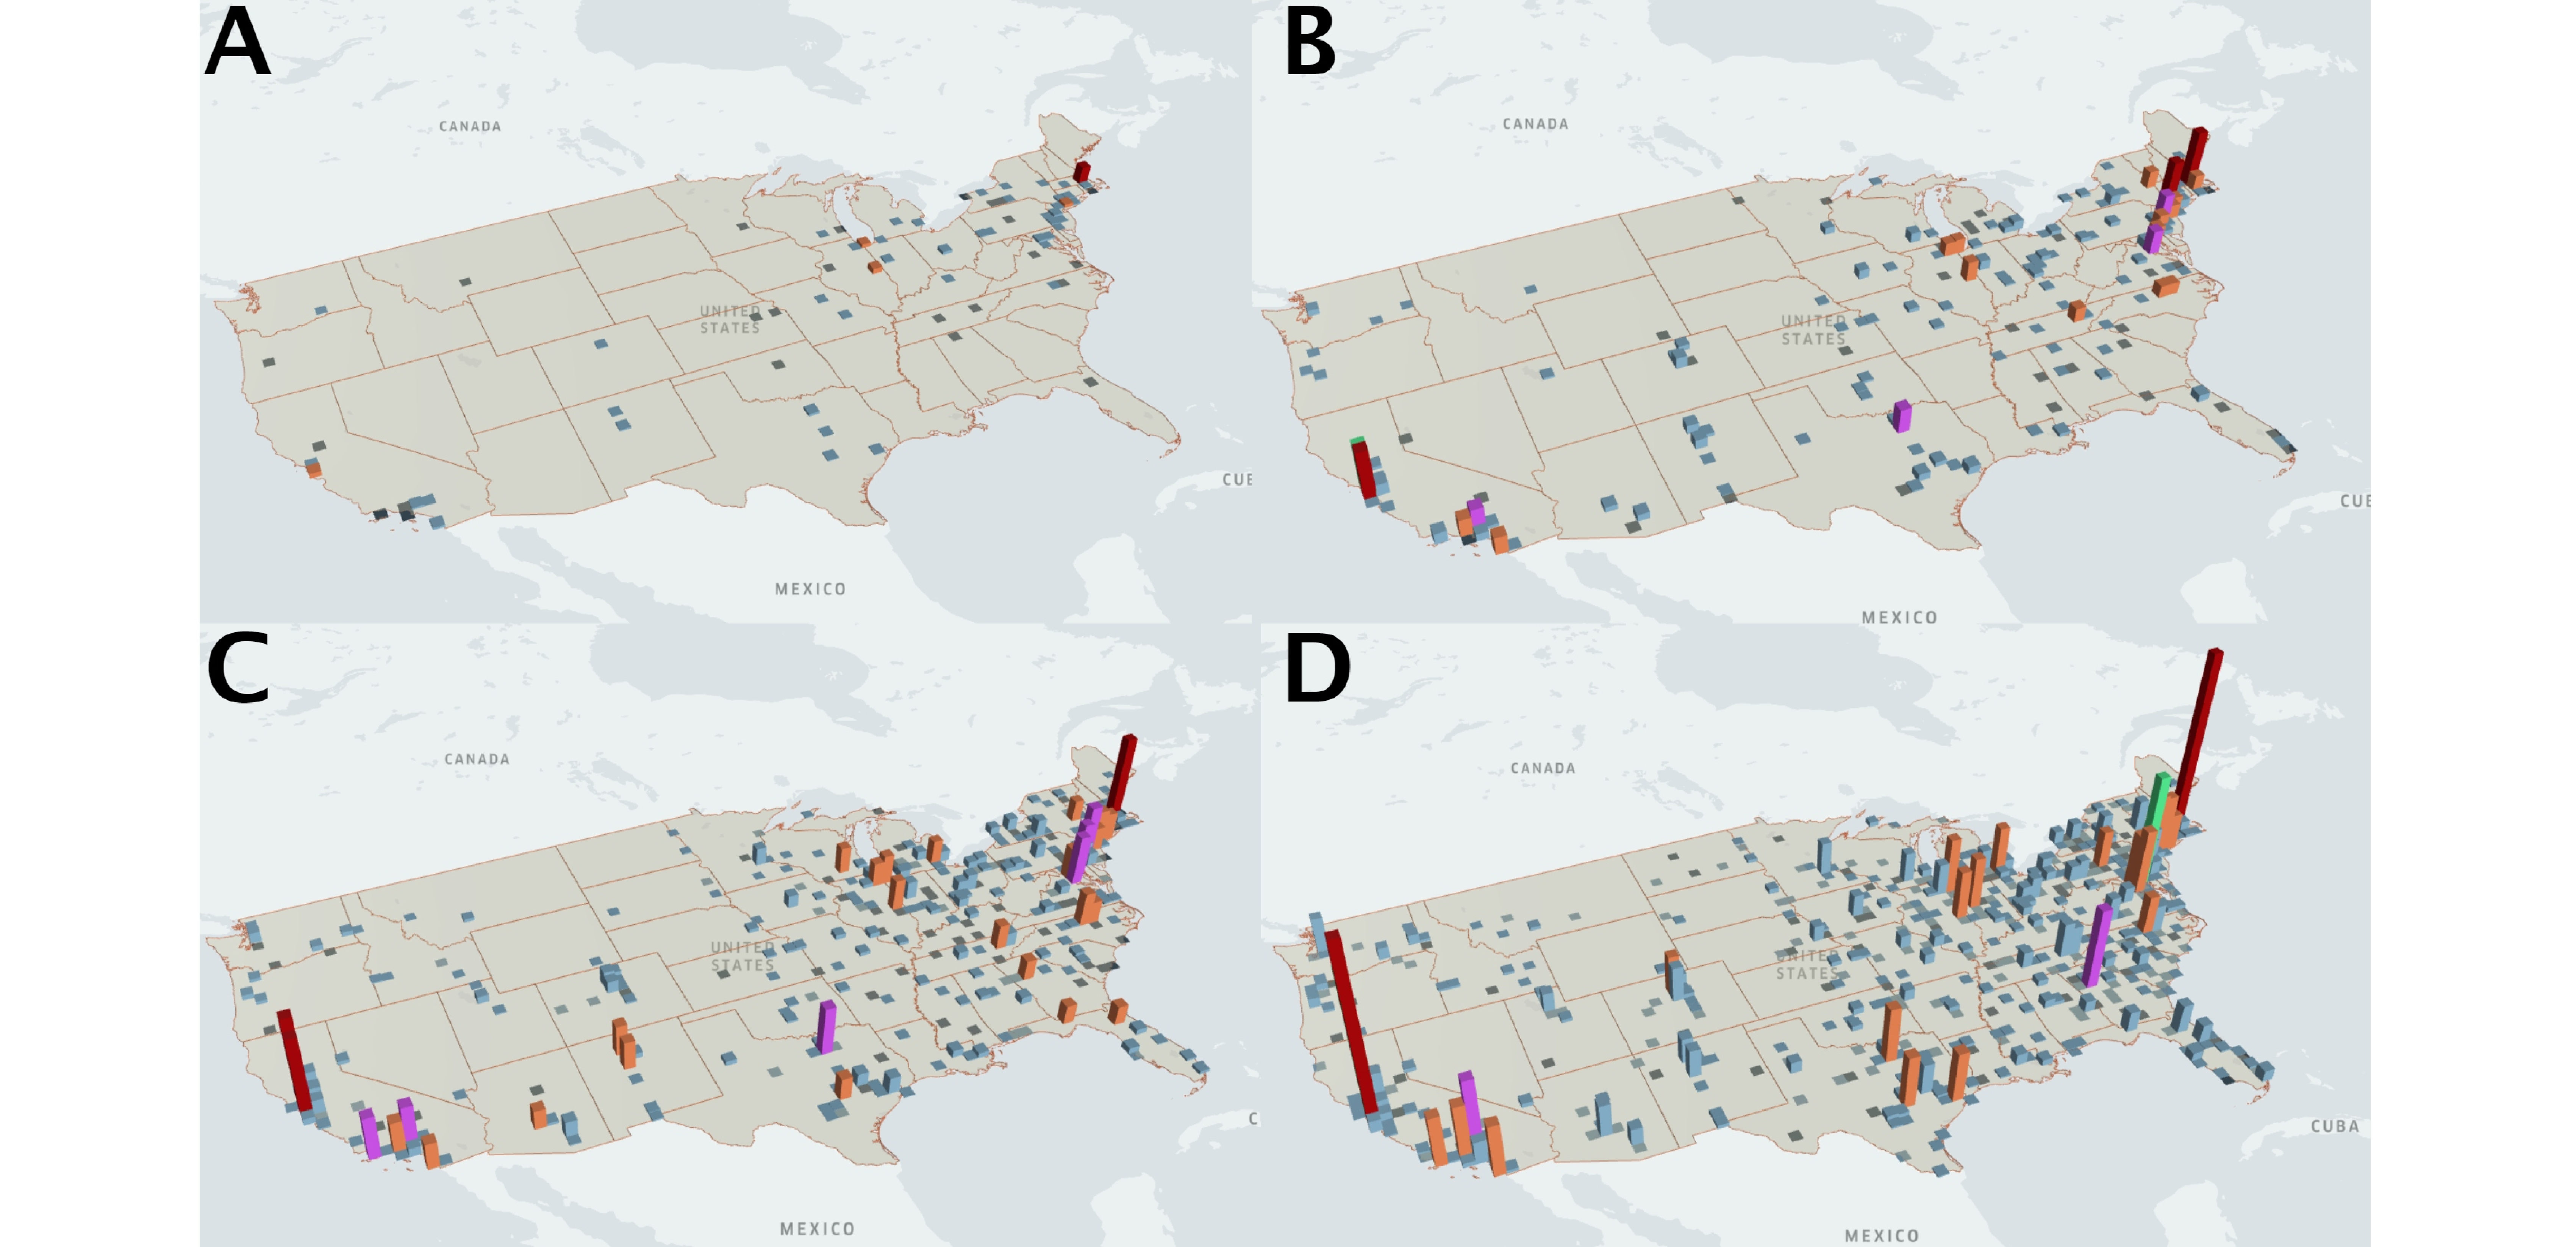
\includegraphics[width=1.0\linewidth]{figures_csf/Figure1_maps.pdf}
\caption{Regional evolution of the number of in-flowing researchers into the field of semiconductors in the US (height of bars) Panels A-D correspond to time periods 1954-1970, 1970-1986, 1986-2002, and 2002-2020, respectively. In the fifties and sixties, only the Boston area plays a role, some researchers are present in Chicago and Silicon Valley. From the seventies on, the Boston area and Silicon valley are dominant; other regions are building up some expertise but never get into a position of becoming a challenger. The five colours (blue, orange, purple, green, and red) indicate steps of 20\% of the aggregated sum of authors' flows value of the inflows at each time period. The respective maximum values for panels A-D are: max = 57, 207, 1086, and 8270. For the definition of a region, see methods Section~\ref{sec:methods}. 
}
\label{Fig1}
\end{figure}

With data extracted from the {\em Dimensions} database, we can reliably reconstruct the changes in affiliations of all researchers in a specific field and infer how they move between geographic regions. We can see which region attracts researchers with certain scientific skills in a time-resolved manner. We see how quickly different regions accumulate specific types of skills over time, which allows us to define regional growth rates of scientific skills. A schematic picture of semiconductor researchers moving into different regions over seven decades is shown in Fig. \ref{Fig1}. The reasons why researchers switch locations are plentiful. In addition to the attractiveness of a region and the everyday surroundings, the scientific environment and the innovation potential also play an important role \cite{trippl2009islands,menter2018search}. This also includes the number of scientists already present in a region \cite{zucker2009star}.

This chapter studies the growth mechanism leading to the observed temporal and regional distributions of accumulated scientific skills in three specific scientific fields: Semiconductor Research, Embryonic Stem Cells, and Internet Research. We identify the underlying mechanism as the so-called ``rich-get-richer'' effect and find no evidence of a critical mass of scientists. In particular, in our analysis of empirical flows of scientists (and their skills ), we find strong evidence for a sub-linear preferential attachment (PA) growth mechanism, meaning that a region becomes increasingly attractive to scientists as the number of existing scientists in a field increases.

Preferential attachment mechanisms (or rich-get-richer or Mathew effect) have been identified in a wide variety of social~\cite{Price76,Simkin11,bol18,capocci06} and network phenomena \cite{Krapivsky00,Newman01,jeong03}. For a  given quantity of interest (integer), $x(t)$, at time $t$, growth following a PA mechanism means that the probability of the quantity gaining one unit within the next timestep is 
\begin{equation}
    \mathcal{P}[  x(t+1) = x(t)+1 ]\propto x(t)^{\alpha} \, .
    \label{eq:genericPA}
\end{equation}
Preferential attachment can appear in linear, sub- and super-linear versions, depending on whether the growth exponent $\alpha=1$, $\alpha<1$, or $\alpha>1$, respectively. Sub-linear PA growth has been reported, for example, in the actor collaboration network and scientific co-authorship networks~\cite{jeong03, Newman01}, as well as in the friendship network formation in a massive multiplayer online computer game \cite{szell11}.
The microscopic mechanisms underlying a sub-linear PA dynamics may be of various types, for example it could be an ageing effect, where scientists prefer newborn institutions, or it could be a fitness-related attachment, where researchers prefer institutions with a high impact, or it could be hiring selection rules, where institutions may lower the entry requirements for the candidates.
A few publications consider these effects in their modeling efforts~\cite{reisz22,wang13,jin19,gleeson14} but do not explicitly relate them to a sub-linear \emph{effective} PA kernel.
In our context we observe that a PA mechanism does not need the knowledge of the entire network for the researchers to move to a region. Picking random scientists (colleagues) and copying their behavior leads to a PA dynamics.
In our study, we do not consider the details of the causes leading to an effective power-law sub-linear PA. We focus on how to measure it and demonstrate its importance for explaining the regional growth of scientific fields.


To test if the conclusion of an underlying effective sub-linear PA mechanism is valid, we design a simple global model of the regional attractiveness of regions to scientists. The model not only replicates the empirical frequency distribution of researchers in different areas but also helps us understand the peculiar behavior of regions that are late adopters of new scientific fields. We illustrate the case of late adopters in the context of semiconductor research, where Silicon Valley intellectually dominated the scene for a long period, from the end of the 1940s on \cite{rao13}. Only very late China entered the scene, starting in the early 1980s. 

From 2006 on, China became the most dominant player in semiconductor research, also thanks to the Chinese ``Me\-dium- and Long-Term Plan for the Development of Science and Technology'' \cite{Lazonick12}. We find that the cumulative number of scientists moving to China and publishing scientific papers exceeds those of California from 2007 on. 
Understanding how this take-over was possible needs special attention –– a naive explanation with PA growth will not be sufficient. Change of leadership is only possible if special action is taken to locally change the PA mechanism with the help of strategic interventions that make regions radically more attractive by investments in technology \cite{Li21} or research and development \cite{tollefson18}. We show that our model can implement these interventions and we quantify how large these efforts have to be to allow regional latecomers to become dominant.

%%%%%%%%%%%%%%%%%%%%%%%
\section{Quantifying PA in academic mobility}
\label{sec:methods}

\subsection{Estimating the PA kernel.}
We estimate the PA attachment probability, $P(k)$, by means of a method originally devised for co-authorship networks \cite{Newman01}. Following this method, we go through the regions in the time-sorted regional stream, $\mathcal{R}$, one by one and build a histogram from which we  estimate the attachment kernel. If a PA process is realized, at each point in time $t$, the probability of a region already occurred $k$ times to appear again is given by
%
\begin{equation}
    \Pi(k,t) = P(k) \frac{n(k,t)}{D(t)} \, , 
\end{equation}
%
where $n(k,t)$ is the number of regions  already appeared $k$ times at time $t$, and $D(t)$ is the total number of regions already appeared irrespective of their number of occurrences. Then, the attachment probability, $P(k)$, can be estimated from a histogram where each contribution is weighted with the inverse frequency  $\frac{D(t)}{n(k,t)}$. The resulting histogram starts to deviate from a straight line (in double logarithmic scale) at around $k\approx60$ (Figs.~\ref{fig:sc-recap} panels A-C). 
This is a well-known behavior of the method. Therefore, we resort to the first 60 points to estimate the exponents with a least squares method in all three scientific fields studied.
In all the three fields we find $R^2 > 0.99$.

\subsection{Determining the PA exponent for Chinese regions.}
We obtain the special value of  $\alpha_\mathrm{CN}=0.915$ in the following way.
We first determine from the data the average growth exponent, $\eta$, exclusively for the Chinese regions obtaining $\langle \eta \rangle_\mathrm{CN}\approx 2.53\pm 0.09$.
Then, from a starting value of $\alpha_\mathrm{CN}=0.79$ --the value of all the remaining regions--  we increment $\alpha_\mathrm{CN}$ in the simulation in steps of $0.005$ until we find an agreement between the empirical $\langle \eta \rangle_\mathrm{CN}$ and the one estimated from the stream of regions  generated by the simulation.

Figures~\ref{fig:sc-intrinsic_growth} C-E and Figures~\ref{fig:sc-model} panels C-E are obtained by first removing all regions with a cumulative number of scientists at the year 2019 less than $100$.
For those regions with a lower number of scientists, the curves of their growth in intrinsic time become noisy, and the estimated exponent  is unreliable.

%%%%%%%%%%%%%%%%%%%%%%%
\section{Results}
\label{sec:results}
%%%%%%%%%%%%%%%%%%%%%%%
We first characterize the mobility of scientists, in particular the growth (and change) of numbers of scientists of a given field working in different world regions. This is based on analyzing the temporal sequences of their publications and affiliations. We define a region as the first-level  administrative division of a country. In the case of the United States, such a region corresponds to a state. For the data collection procedure, see \ref{app:data}; for an overview of the data set, consult Tab.~\ref{tab:fields}. 
\begin{table}[tb]
    \centering
    \caption{Descriptive features of the data set used in the three studied scientific fields. 
}
    \begin{tabular}{l c c c }
                &  Semiconductors  & ESC & Internet \\
    \hline
starting year   & 1941      & 1941      & 1956      \\
end year        & 2019      & 2019      & 2019\\
researchers     & 2,011,170 & 752,575   & 109,098   \\
articles        & 5,062,639 & 1,083,100 & 246,953   \\
regions          & 1,633    & 1,161     & 1,032     \\
Heaps' exp. $\gamma$    & 0.39     & 0.37  & 0.48  \\
PA exponent  $\alpha$    & 0.79     & 0.84  & 0.79  \\
\end{tabular}
    \label{tab:fields}
\end{table}

%\vspace{1mm}\noindent\textbf{The data.}
To arrive at a practical data structure for the analysis, we define an event, $E(T)$, as a publication of an article in a given field of research at time $T$ (date of publication) by a scientist. It consists of four entries,  $E(T)=(S, R, T, F)$, the scientist, $S$, the region, $R$, with the condition that $S$ has published in the region $R$ for the first time (i.e., the pair $(S,R)$ has never occurred before, and the scientific field is $F$. We skip an event for which this condition is not fulfilled. 
We ensure that we only record the scientists that move into a new region or who start their careers. 

Our work focuses on academic mobility from the perspective of receiving countries and regions. Since we mainly focus on how regions receive new people in specific scientific domains, we do not account for returned mobility (i.e., people who return to a location where they previously have become ``attached'' to).  Post-migration retention, attrition, and returning are highly significant dimensions of the knowledge transfer equation and are ideal for follow-up studies focusing on questions of \emph{brain circulation} and strategies to mitigate the effects of \emph{brain drain}. We do not deal with these themes here.

One publication may generate multiple events according to the number of scientists in the author list. 
%
Here, we consider a full counting of all authors and their affiliations (and regions) recorded in the publications.
Note that a ``fractionalization'' of researchers' and regions' contributions to papers, where researchers and regions are assigned a relative weight, makes little sense in the present context since we build sequences of events. Moreover, fractional counting is usually not considered when the analysis is conducted for a single discipline, nor when studying mobility flows, as in our case~\cite{garcia19,waltman15,moed05}.
%
After sorting events, $E(T)$, ascending in time, we get a sequence, $E_t$, where $t$ is an index that indicates the event's position in the sequence. We call $t$ the \emph{intrinsic time}. For every index, $t$, there is an associated time, $T$, given by a non-decreasing function $T(t)$. Intrinsic time is a convenient way for treating sequences of events whenever their rate of appearance in real-time is not constant. This is indeed the case since, in most fields, the number of published articles increases exponentially in real-time \cite{reisz22}, and, correspondingly, the real-time difference between two consecutive articles decreases exponentially. 
%
We can consider the derivative of intrinsic time with respect to real-time, as a proxy for attractiveness of new locations. 
We increase intrinsic time whenever someone moves to a new location in their life. This means that the field has to be sufficiently attractive to justify a person with their family to move or to justify the addition of a new affiliation to one's list.

%
From the sequence, $E_t$, we extract the corresponding sequences of regions, $R_t$,  which we call \emph{regional stream}, $\mathcal{R}$. For example, 
see Tab~\ref{tbl:stream}.

\begin{table}[t]
    \centering
    \caption{Sequence of publication events, $E$,  in the field of physics. Intrinsic time increases by one each time a scientist publishes an article in a given region for the first time. From this data, all necessary sequences can be extracted. In the specific example, Bob has already published in Arizona at intrinsic time $t=2$, so all his future publications in Arizona no longer appear in the stream. Using initials for regions, this example generates  the regional stream, $ \mathcal{R} = (A,A,A,C,A,D,C)$.
}
    \begin{tabular}{ c c c c c c }
\textbf{} & \textbf{real} & \textbf{intr.} & \textbf{} & \textbf{} & \textbf{} \\
\textbf{paper} & \textbf{time} & \textbf{time} & \textbf{scientist} & \textbf{region} & \textbf{field} \\
    \hline
article 1 & 1960 & 1    &   Alice   & Arizona   & phys.    \\
article 1 & 1960 & 2    &   Bob     & Arizona   & phys.    \\
article 1 & 1960 & 3    &   Charlie & Arizona   & phys.    \\
\hline
article 2 & 1961 & 4    &   David   & California    & phys.\\
\hline
article 3 & 1961 & ---  &   Bob     & Arizona    & phys.   \\
article 3 & 1961 & 5    &   David   & Arizona    & phys.   \\
\hline
article 4 & 1962 & 6    &   Alice   & Delaware  & phys.    \\
\hline
article 5 & 1963 & ---  &   Bob       & Arizona   & phys.    \\
article 5 & 1963 & ---  &   David     & Arizona   & phys.    \\
article 5 & 1963 & ---  &   Alice     & Arizona   & phys.    \\
\hline
article 6 & 1964 & 7    &   Bob       & California & phys.   \\
    \hline
\end{tabular}
    \label{tbl:stream}
\end{table}

Given a regional stream, one defines two useful quan\-tities. First, the cumulative number of new scientists who moved into the region $i$ (or started their publishing career there), before time $t$ 
\begin{equation}
    k_i(t) = \sum_{\tau=1}^{t} \delta(R_\tau, i)\, ,
    \label{eq:degree}
\end{equation}
where $\delta(x,y)$ is the Kronecker symbol, $\delta(x,y)=1$ if $x=y$ and zero, otherwise. The second quantity is the number of different regions appearing in the regional stream before time $t$
\begin{equation}
    D(t) = \sum_{\tau=1}^{t} \delta(k_{R_\tau}(\tau), 1)\, .
    \label{eq:dictionary}
\end{equation}
$D(t)$ is the number of regions appearing at least once and resembles the ``regional diversity'' of a field. We only focus on the number of papers published within a region and ignore their impact and quality. 

\vspace{1mm}\noindent\textbf{The sub-linear PA kernel.} 
From the time evolution of the quantities, $k_i(t)$, we can estimate the probability for a scientist to move to a new location of work (and publish there for the first time) that has already had $k$ scientists up to time $t-1$:
\begin{equation}
    P_k(t) = {\mathcal{P}} \left[k_i(t)=k+1 \;|\; k_i(t-1)=k\right]\, .
    \label{eq:attachmentprobability}
\end{equation}
For simplicity, we assume that $P_k(t)$ does not explicitly depend  on time, $t$, but on the number of occurrences, $k$, of the regions in the regional stream, and we write $P_k(t)\approx P(k)$. We will see that this approximation already explains the experimental data well. We estimate $P(k)$ with the running histogram method \cite{Newman01},  briefly described in the methods Section~\ref{sec:methods}.

\begin{figure}[!htb]
\centering
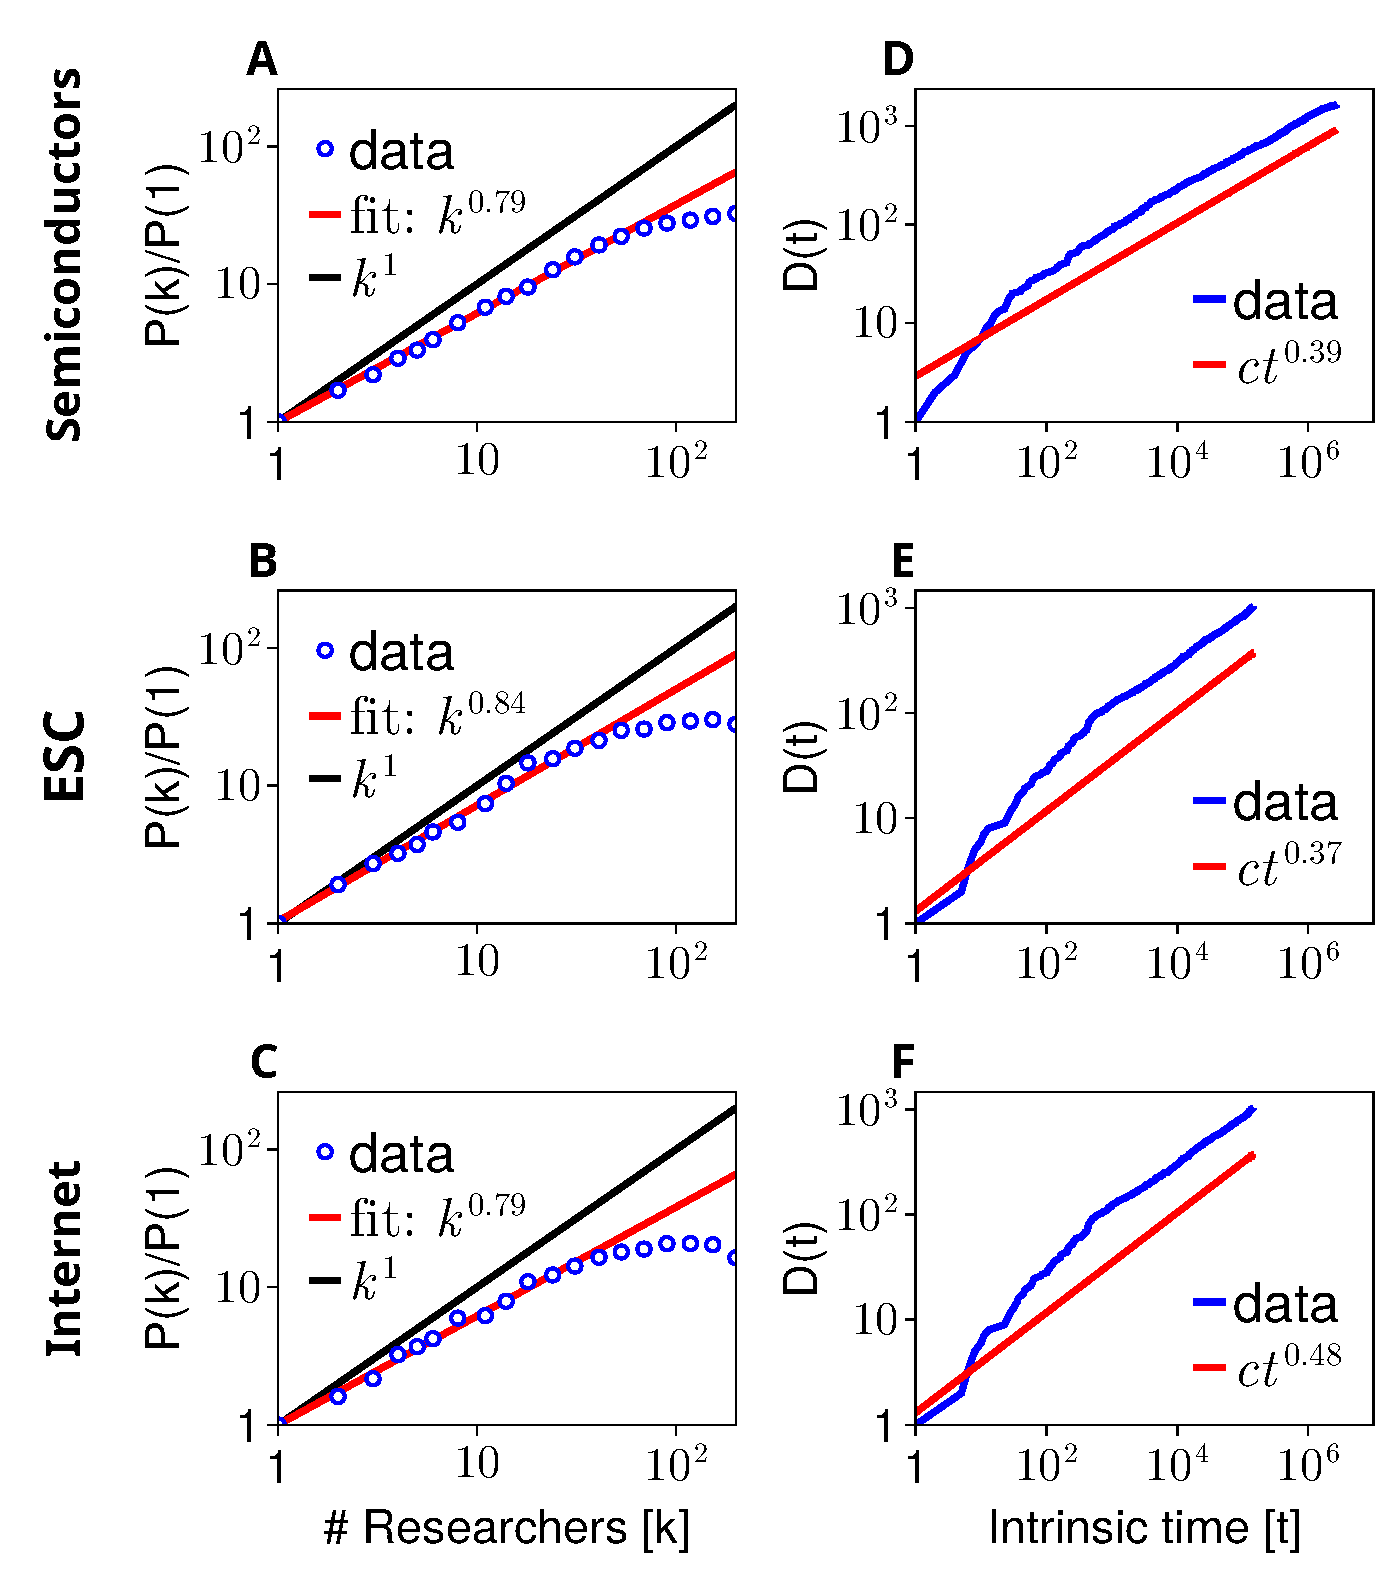
\includegraphics[width=0.8\linewidth]{figures_csf/fig2.pdf}
\caption{Growth statistics of the three fields. 
Panels A-C show the probability for a scientist to move into a region where $k$ researchers are present. The attachment probability, $P(k)/P(1)$ (PA kernel), (blue) shows a sub-linear power-law increase as a function of $k$. The least-square fits are shown in red, the black line indicates the linear exponent, $\alpha=1$. 
(A) shows the case for semiconductor science, B for ESC, and (C) for Internet research. 
For the sake of readability, in panels A-C we show only data for small $k$ where we find an approximately linear relation in the log-log plot. 
We do not show data for $k>200$ where curves drop due to insufficient statistics. Panels D-F shows the increase of regional diversity, $D(t)$, occurring in the regional stream, $\mathcal{R}$, as a function of intrinsic time, $t$ (blue). After an initial transient, $D(t)$ approaches an approximate power-law (Heaps' law).}  
\label{fig:sc-recap}
\end{figure}

In Fig.~\ref{fig:sc-recap} panels A, B, and C, we show the empirical settlement probabilities, $P(k)$, for a scientist (in the fields of semiconductor research, embryonic stem cells, and Internet research, respectively) to move to a new location of work and publish there for the first time -- as a function of the number of scientists who already work in that region, $k$. The probability is normalized by $P(1)$; we call $P(k)/P(1)$ the effective {\em attachment kernel} \cite{Pham15}. 

Clearly, with increasing numbers of already present scientists, a power-law increase of the attachment kernel is visible. The attachment exponents, defined in Eq.~(\ref{eq:genericPA}), are $\alpha\sim 0.79$ for semiconductor and Internet research, and $0.84$ for ECS (see Table~\ref{tab:fields}). For reference, the black lines indicate the linear PA mechanism, i.e., $\alpha=1$. 

Panels D, E, and F of Fig.~\ref{fig:sc-recap} show the number of different regions appearing in the stream $D(t)$ as a function of intrinsic time. After a brief linear transient that ends around $t\approx 100$ publications in all three fields, $D$ increases as a power-law, $D(t)\approx t^\gamma$, with $\gamma<1$. The initial linear growth, which is the fastest growth possible in intrinsic time, reflects the fast diffusion of the three scientific fields across the world at their onset. As time goes on, the initial constant rate, $\frac{d}{dt}D(t)$, turns into a time decreasing regime with an exponent $\gamma-1$. We observe no saturation effects at high intrinsic times despite the number of different regions in the three cases has crossed (semiconductors, embryonic stem cells), or is close to (Internet), the 50\% of the total number of regions in the world, i.e., 2,092 in the year 2019.

A power law increase in novel entries in a stream has been associated with the existence of the so-called {\em Heaps' law} that often appears in evolutionary time series \cite{Serrano09,Tria14,Mazzolini18,Tria18,Simini19}. In the present case, Heaps' law shows how fast a new scientific field spreads in regions around the globe.

\subsection{Growth of regional capacity}
\begin{figure}[!htb]
\centering
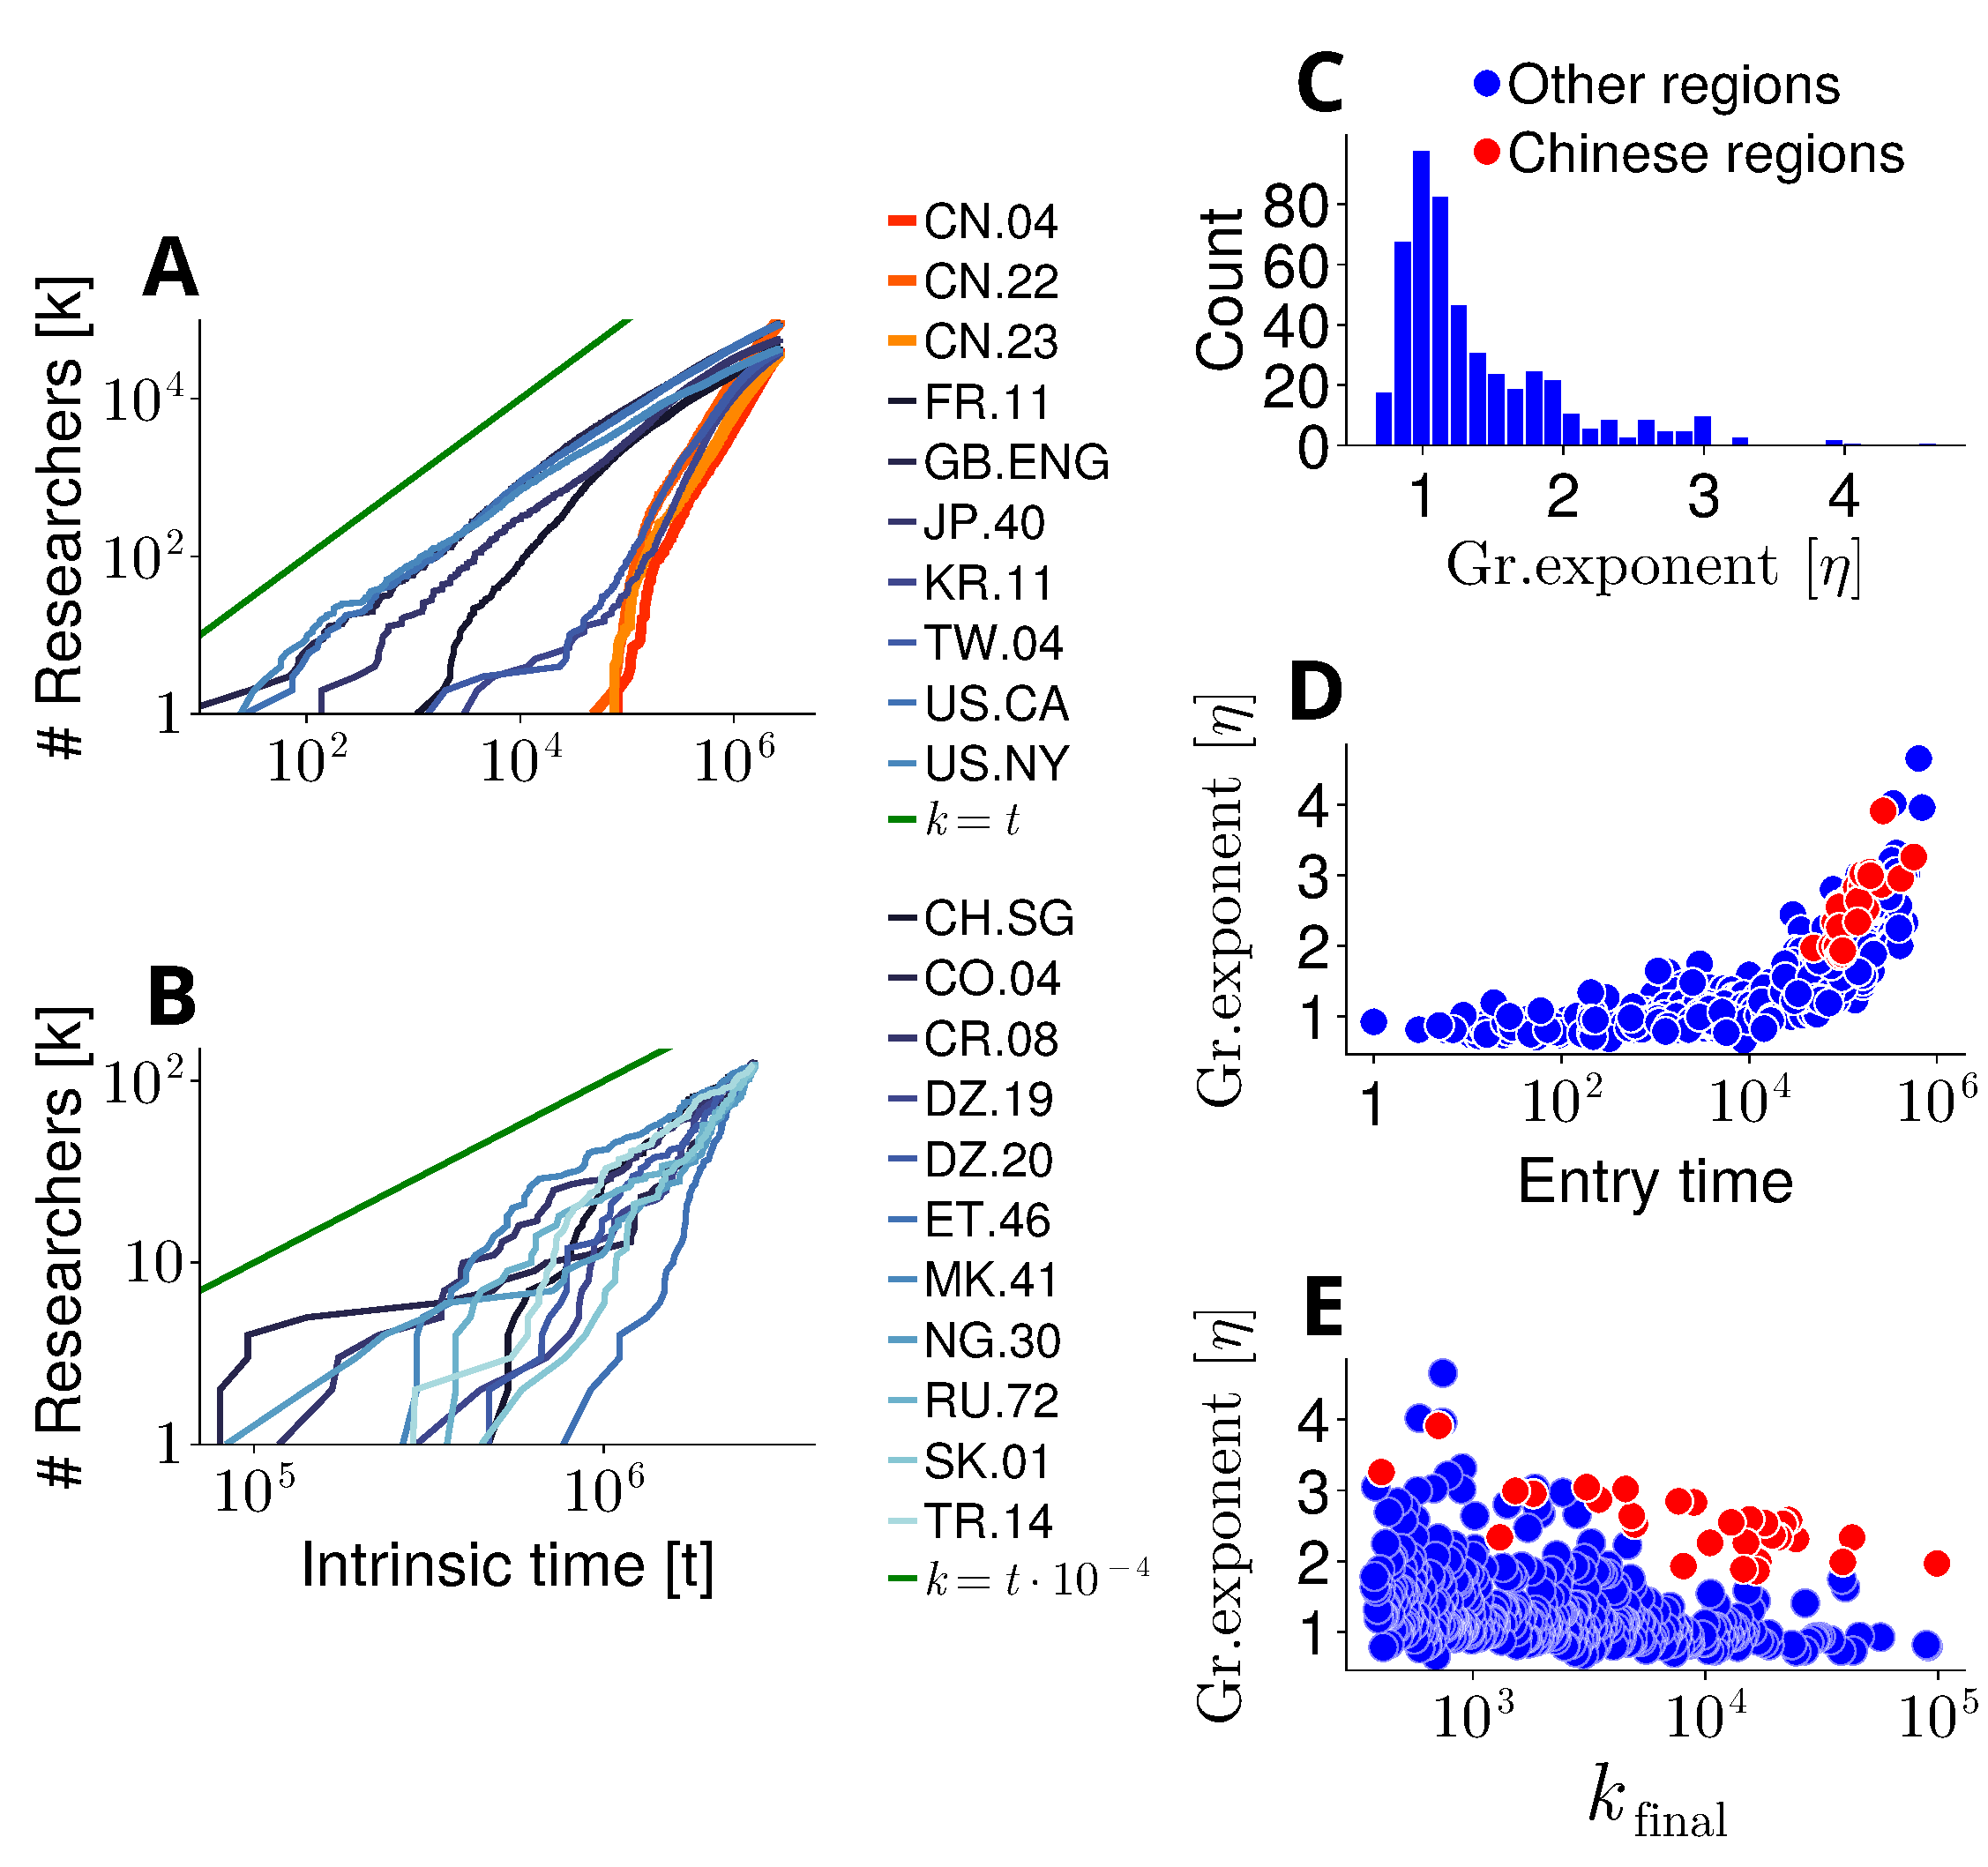
\includegraphics[width=0.8\linewidth]{figures_csf/fig3.pdf}
\caption{Panels A and B show the cumulative number of scientists coming into a region (lines) in intrinsic time in semiconductor research; (A) shows the 10 most visited regions. Most regions grow sub-linearly. Chinese regions are shown with red thick lines and increase super-linearly.
In (B), we see 11 poorly visited regions ranked from 700 to 710 regarding the number of scientists. Curves are (additively) shifted to the left so that their first point is placed at coordinates (1,1);
In both (A) and (B), the green straight lines on the top represent the linear regime.
(C) Histogram of growth exponents, $\eta$, for all regions;
(D) Growth exponents, $\eta$, of all regions, $i$, as a function of their entry time, $t_i$ (intrinsic time). Note that Chinese regions (red) come in late (after timestep $10^5$) and have higher exponents than other regions (blue).
(E) Growth exponents, $\eta$, as a function of the cumulative number of scientists in 2019, $k_{final}$. The high exponents of Chinese regions are visible (red).
} 
\label{fig:sc-intrinsic_growth}
\end{figure}
 
In Fig.~\ref{fig:sc-intrinsic_growth}, we show the cumulative number of semiconductor scientists working in several selected regions in intrinsic time. We do not distinguish those scientists leaving a region for a new one from those who start in a region for the first time in their career in the semiconductor field. We fit with a least square procedure the regional growth curves with $k(t) \sim t^{\eta}$, where $\eta$ is the {\em growth exponent}, that can be interpreted as the {\em regional growth capability}.
In all the three scientific fields we find $R^2 > 0.9$ for the $\eta$ fits, with very few values between 0.85 and 0.90.

In panel A, every curve represents a region that belongs to one of the 10 most successful ones (cumulative number of scientists in the order of $10^5$). Most curves grow sub-linearly with the exception of the three regions in China (denoted by CN.\{04,22,23\}); these grow faster than linear (left-bent). Both California (US.CA) and England (GB.ENG) have an exponent of approximately $0.8$  (yellow and green curves practically overlap), while the Chinese region around Beijing (CN.22) shows an exponent of about $1.8$. This means that Chinese regions follow a very different growth pattern. Note that Chinese regions entered the scene only after about 90,000 papers were published in the field, corresponding to the year 1977. 

In panel B, we show the growth curves of 11 low-ranked regions (rank 700-710). These all have a final cumulative number of scientists of about 120. All of them grow super-linearly with an exponent of approximately $1.6$. The general trend is that well-established regions  in a field generally grow sub-linearly (curves bent to the right), while late adopters grow super-linearly. 

Figure~\ref{fig:sc-intrinsic_growth} C shows the histogram of the growth exponents, $\eta$, for the semiconductor case. 
We find a distribution with mean $m = 1.55$, standard deviation $s = 0.69$ and skewness $b=1.52$. 
 For the other fields the situation is similar:
 Internet: $m=1.36$, $s=0.59$ and $b=1.48$; 
 embryonic stem cells: $m=1.56$, $s=0.86$ and $b=1.73$.

In Fig.~\ref{fig:sc-intrinsic_growth} D we show the growth exponents, $\eta$, of all world regions, $i$, as a function of their entry time, $t_i$, defined as the time (measured in intrinsic time) at which a region appears in the affiliation list of an article for the first time. Exponents are larger the later a region enters. Late adopter regions seem to bring in scientists faster than regions where the field started. Yet, in most cases, higher exponents are not enough to catch up and challenge the leaders in the field. Chinese regions are marked in red. They come in late ($10^5$) and have exponents higher than other regions (blue). 

Finally, in Fig.~\ref{fig:sc-intrinsic_growth} E we see the regional growth exponents, $\eta$, as a function of the cumulative number of  scientists up to year 2019 in a region, $k_{final}$. The visual general decay means that the more scientists are present in a region, the lower is its growth capability. Note again the exceptionally high growth exponents for the Chinese regions.

\subsection{Relations between the three exponents}
The exponents $\alpha$, $\gamma$, and $\eta$ are related. The corresponding functional expressions can be estimated with simple reasoning, see \ref{app:scaling}, or are obtained through an approximate analytic solution of the model, see \ref{app:analytical}.
 
\subsection{A simple generative model}
To understand the observed statistical features presented in Figs.~\ref{fig:sc-recap} and \ref{fig:sc-intrinsic_growth}
we devise a simple model. We first specify a scientific field, e.g., semiconductor research. We use the empirical regional stream, $\mathcal{R}$, as the baseline to build a new synthetic stream, $\mathcal{S}$. We start at $t=0$ with the first region, $R_0$, where a scientist's affiliation in an article appeared for the first time. We insert this region in $\mathcal{S}$ as its first element $S_0$. For each following intrinsic time, $t>0$, we add an element $S_t$ in $\mathcal{S}$ in the following two ways according to whether $R_t$ has already appeared in $\mathcal{R}$ or not: 
\begin{itemize}
\item if region $R_t$ has never appeared in $\mathcal{R}$ before, i.e., $k_{R_t}(t)=1$, we also insert it in $\mathcal{S}$, so that $S_t\equiv R_t$;
\item if region $R_t$ has already appeared in $\mathcal{R}$, i.e., $k_{R_t}(t) > 1$, we randomly select a region $s$, from those regions already in the stream $\mathcal{S}$, with a preferential attachment probability
\begin{equation}
    \begin{array}{rl}
        P_k(t) &= {\mathcal{P}} \left[k_s(t)=k+1 \;|\; k_s(t-1)=k\right] = \\
            &= Z^{-1}{k^\alpha} \, , \nonumber
        \label{eq:kernel}
    \end{array}
\end{equation}
where $Z(t)=\sum_{s=1}^{D(t)} k_s^\alpha(t)$ is a normalization term. In other words, we choose regions with a probability proportional to a power, $\alpha$, of their number of occurrences in $\mathcal S$ until time $t-1$.
\end{itemize}

Since the entry times of new regions in the two streams,  $\mathcal{R}$ and $\mathcal{S}$, are the same by construction, the number of different regions in time, $D(t)$, coincides in the two streams, meaning that also Heaps' law is the same (Fig.~\ref{fig:sc-model} B). The model has one free parameter, the PA attachment exponent, $\alpha$, of the sub-linear PA mechanism. Note that this model is similar to the one presented in \cite{Zanette05} where, however, the PA was linear. The model can be approximately solved analytically; see \ref{app:analytical}.

For the bulk of the model simulations, we chose $\alpha$ as measured in the data, i.e., $\alpha=0.79$, $0.79$, and $0.84$ for the Internet, semiconductors, and stem cell areas, respectively; see Table~\ref{tab:fields}. For this choice, a run of the model for the semiconductor research followed by a simple linear regression yields  $\gamma\approx0.39$ and $\eta\approx0.74$.

\subsection{Understanding exceptional super-linear regions}
\begin{figure}[!ht]
    \centering
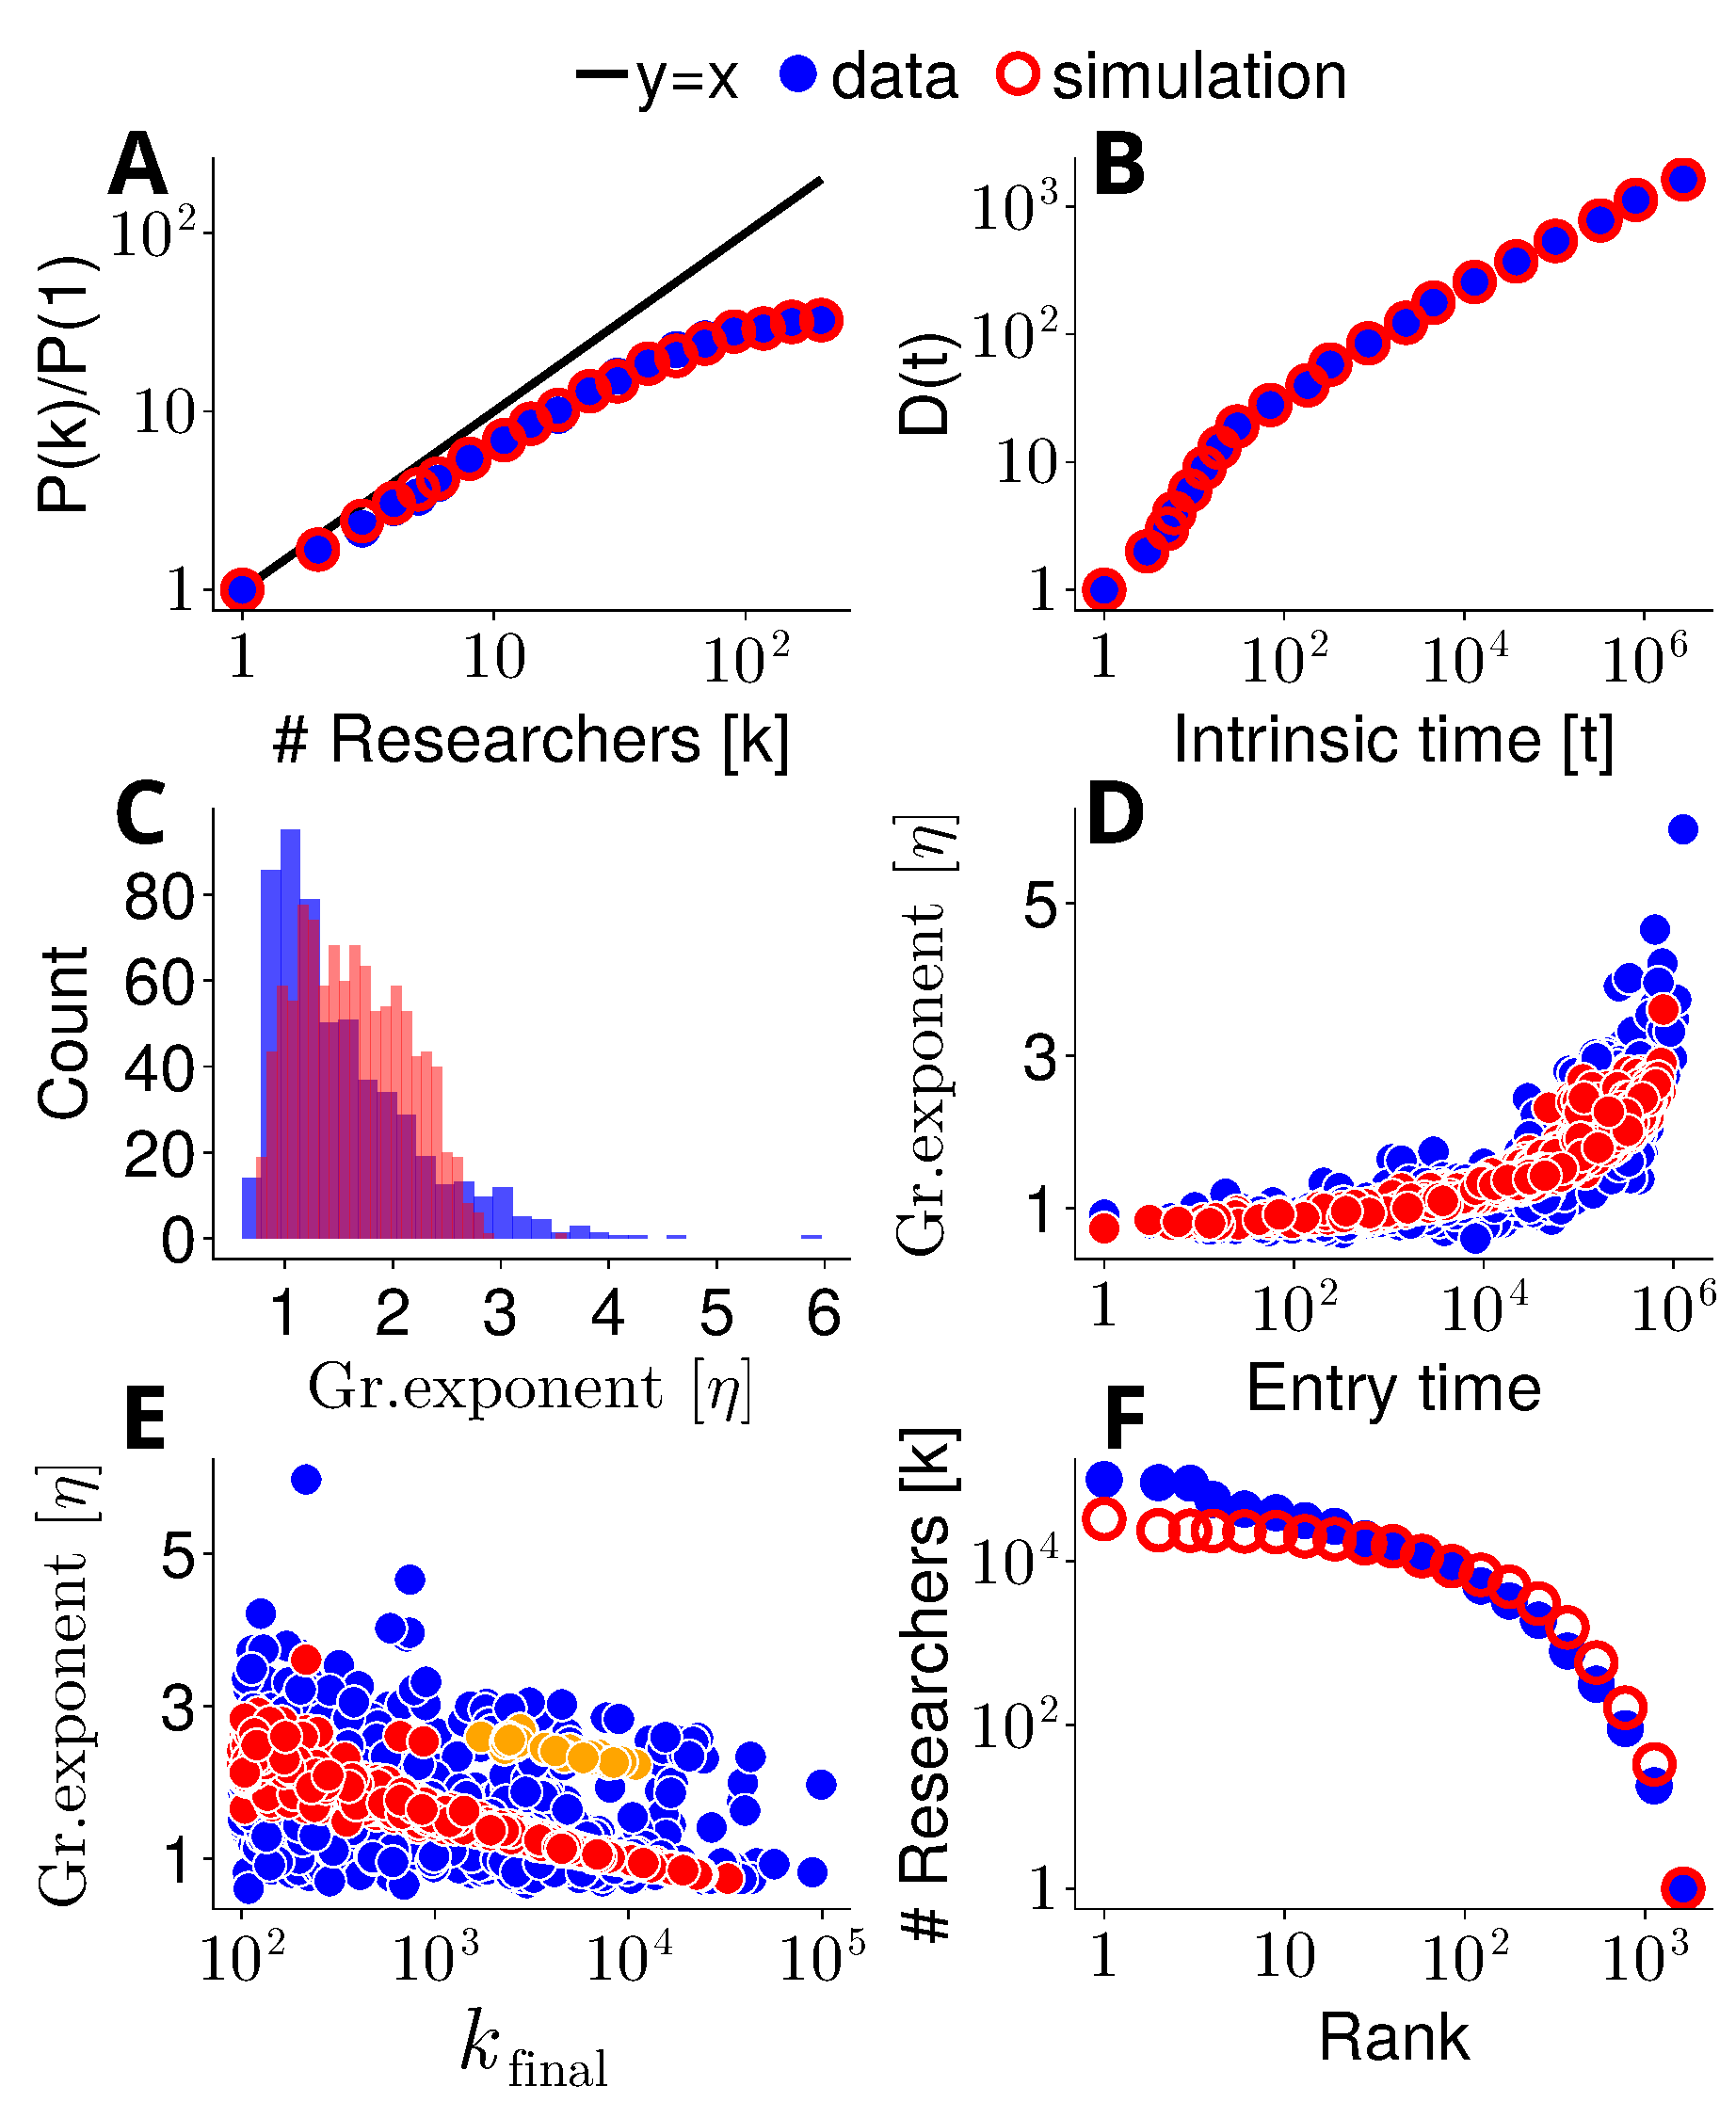
\includegraphics[width=0.7\linewidth]{figures_csf/fig4.pdf}
    \caption{Comparison of model results (red) with experimental data  (blue) for the field of Semiconductors.
    (A) PA kernel; data and simulation practically coincide; the black line depicts a linear kernel.
    (B) Heaps's law; the two curves coincide by construction.
    (C) Histograms of the regional growth exponent, $\eta$. Simulations show a slightly higher mean. 
    (D) Exponents, $\eta$, reproduce the empirical increase as a function of entry time.
    (E) The decrease of $\eta$ as a function of the cumulative number $k_\mathrm{final}$ of scientists in the year 2019 is well captured by the model. Note the fact that Chinese regions (orange circles) are predicted with higher than usual values.
    (F) Also, the frequency-rank distributions of the regions appearing in the two streams practically coincide except for very small ranks.
    In panels C, D, and E, only regions with $k_\mathrm{final}>100$ are taken into account.
    }
    \label{fig:sc-model}
\end{figure}
To model the exceptional super-linear growth of Chinese regions in the field of semiconductors, visible as the red curves in Fig.~\ref{fig:sc-intrinsic_growth} A, we use as an input a slightly larger PA exponent $\alpha_\mathrm{CN}=0.915$ for these regions only, while for all the other regions we keep $\alpha=0.79$, see the methods Section~\ref{sec:methods}.

In Fig.~\ref{fig:sc-model}, we compare the model results (red) with the empirical data (blue). In panel A, we show the PA kernel, as in Fig.~\ref{fig:sc-recap}, panels A, B, and C. 
In the simulation, we use the empirical value of the PA exponent of $\alpha=0.79$ for all the 1633 regions (except the 31 Chinese regions for which we use $\alpha_\mathrm{CN}=0.915$). The two curves almost coincide even for $k>60$, i.e., outside the interval used to fit $\alpha$. This confirms the goodness of the fit.

In Fig.~\ref{fig:sc-model} B, we plot the  number of distinct regions, $D(t)$, as a function of intrinsic time, in the regional, $\mathcal R$, and the synthetic stream, $\mathcal S$. Since the entry time of new regions is the same in both streams, the two curves are identical.

Figure~\ref{fig:sc-model} C compares the distribution of the growth exponents, $\eta$. 
In the simulation, the distribution has a somewhat higher mean than the data and lower skewness; we get mean $m = 1.63$, standard deviation $s=0.49$ and skewness $b=0.28$. 
For the data we found $m=1.55$, $s=0.69$ and $b=1.52$. 
The model under-populates the large exponents and underestimates the small ones.


In Fig.~\ref{fig:sc-model} D, the growth exponent at the entry time of a given region is plotted against the entry time in intrinsic time. The simulation results explain the data, particularly that latecomers tend to have higher growth exponents. 

Figure~\ref{fig:sc-model} E shows the comparison for the growth exponent, $\eta$, as a function of the cumulative number of researchers in a region in 2019, $k_{ final}$. The more scientists are present, the smaller the growth exponent. Fewer scientists correspond to higher entry times and, thus, to higher exponents. The red circle marks the Chinese regions in the model to which we assigned higher $\alpha$ values. Also, for these, the model practically reproduces the data. 

Finally, Fig.~\ref{fig:sc-model} F gives the frequency rank distribution of the regions appearing in the two streams. The model also reproduces the distribution obtained from data well. A consequence of a sub-linear PA is that the corresponding frequency-rank of the cumulative number of distinct scientists who worked in a region is not an exact  power-law~\cite{Krapivsky00} -- a fact that we hereby verify. 

In \ref{app:embryo} and \ref{app:internet} we show the results for the embryonic stem cells and Internet research in the same manner as in Figs. \ref{fig:sc-intrinsic_growth} and \ref{fig:sc-model}.


%%%%%%%%%%%%%%%%%%%%%%%

\section{Discussion}
\label{sec:discussion}
Using metadata from scientific publication databases, we reconstructed the regional cumulative number of publishing scientists across the world regions. We find that researchers tend to move to regions according to a sub-linear PA mechanism, where the settling probability for a region is proportional to a power of the cumulative number of scientists already working in that region. In other words: We find evidence for the rich-get-richer phenomenon of scientific mobility of a sub-linear type. This means that regions that move early-moving are likely to dominate the field (or become one of the few dominant regions) and then retain that dominance for a long time.

We find power-law-like regional growth curves that indicate the absence of any specific scale that would reflect the presence of a critical mass. We find no signs of a critical mass (or density) of scientists in a particular topic necessary before the field takes off regionally; a simple PA model is sufficient to explain the main features of the data.

The number of researchers in early-moving regions tends to grow sub-linearly in intrinsic time. The more researchers there are, the lower the regional growth rates. Latecomer regions, which start attracting researchers at a later stage (after the first several hundred articles have been published), are characterized by a number of researchers that can be several orders of magnitude smaller than that of pioneer regions. We find evidence that latecomer regions tend to grow faster, typically even superlinearly, in their initial phase, but with numbers so small that they can practically never even approach dominance. The exponents of regional growth increase with the delay of entry into the field relative to the age of the discipline. Since regions that have been in research for a long time have higher cumulative numbers of scientists than regions that enter late, regional growth exponents tend to decrease as more scientists populate the region. We demonstrate the existence of the same generic mechanism in three different scientific domains over many decades.

For these three domains, we find that Chinese regions behave differently from all the others. They do not follow the sub-linear growth of the pioneering regions but grow super-linearly (in intrinsic time), starting after $500,000$ articles have been produced in the field. This suggests that Chinese regions follow a different pattern.
The simplest way to explain the differences is to assign them a higher PA exponent -- still being sub-linear. This means that as compared to the other regions, Chinese ones attract scientists with higher probability.
We speculate that Chinese regions become more attractive thanks to strategic efforts, including proactive hiring policies, massive funding, and by training a huge reservoir of scientists abroad and bringing them back.
We emphasize that the PA exponent does not depend on the multiplicity of Chinese scientists (population effect) since it determines how researchers attach to a region. In the first approximation, the PA mechanism does not depend on the number of attaching nodes. Of course, there could be an indirect effect by which the high number of scientists requires the introduction of \emph{ad hoc} policies. 
Figure~\ref{fig:sc-intrinsic_growth}~E shows how the growth exponents decrease with the final number of scientists, with Chinese regions being the outlier red circles.

Introducing a higher PA exponent for Chinese regions in our model yields the correct massively larger growth exponents, $\eta$, that are observed. The deeper reasons why Chinese regions behave differently by attracting researchers more strongly than others -- still under a PA scheme -- have to be investigated in future research.

Note that the study considers all regions as having the same PA exponent, except for the Chinese regions that have a larger one. 
This is a gross simplification. However, it still explains the data reasonably well. Nevertheless, the shortcoming of identical exponents should be addressed in future work by a more precise description that assigns different exponents to different regions, ideally on an empirical basis. How this can be done is not so clear. 

Finally, we mention that, remarkably, we find that the rate at which regions join a specific field follows an approximate power-law. This feature has been referred to as Heaps' law that occurs in numerous evolutionary processes \cite{Serrano09,Tria14,Mazzolini18,Simini19}. 
Heaps' law is intimately connected to the idea of the adjacent possible~\cite{Tria18}, where the discovery of new things or ideas leads to other discoveries and results that were impossible to achieve before~\cite{Kauffman00}.

In summary, our simple PA model captures the essence of the underlying preferential attachment process. To a large extent, it explains the empirical data of the historical evolution of the three studied disciplines. It captures both the growth of scientific capacity in individual regions and the observed super-linear initial growth of latecomer regions. The model is simple enough to be analytically tractable, which allows for a detailed understanding of the relations between the three  power-law exponents involved in the process. In particular, it explains why faster growth of latecomer regions is observed. 

The popular explanation that attaining (or catching up to) leadership in a scientific discipline requires building a critical mass of scientists is not supported by data on scientific mobility. We conclude that there are two ways to secure leadership and scientific dominance in a field: One is to have a strong presence among the earliest and earliest players, which is entirely consistent with the theory of increasing returns \cite{arthur89}. The other is to ensure the continuation of exceptionally high, superlinear growth rates through strategic interventions that must be sustained over long periods of time (decades). The latter has been most evident in some areas of Chinese science: The beginning of the catch-up process in the late 1970s led to a dominant role today.

\newpage

\section{Supplementary information}
\subsection{Establishing the data set}
\label{app:data}

\textbf{The Dimensions data.}
\noindent
 We access the {\em Dimensions} database through the Centre for Science and Technology Studies (CWTS), Leiden University. Dimensions covers millions of research publications connected by more than 1.6 billion citations, supporting grants, datasets, clinical trials, patents, and policy documents. In this work, we only use research publications. The publications database of Dimensions contains publication data spanning several decades. The database comprises about 20 million disambiguated researchers assigned to a researcher ID. It also comprises affiliation linkages to the Global Research Identifier Database that currently covers more than 98,000 research institutions worldwide\cite{hook2018dimensions, herzog2020dimensions}. 
{\em Dimensions} is produced by Digital Science and launched in January 2018. For further references, see the Dimensions.ai website\footnote{\texttt{https://www.dimensions.ai/}}.
%\href{https://www.dimensions.ai/}{Dimensions.ai website}

\textbf{Preparing the data.}
\noindent
We start by collecting documents (i.e., all document types) in three different topics, i.e., Semiconductors, Embryonic Stem Cell (ESC) research, and Internet research. 
We chose these areas since they are sufficiently large and important to provide a meaningful statistical analysis. 
% Topic identification 
Delineating research areas is crucial to study their growth. Different types of data and techniques have been proposed to delineate research areas such as document co-citation \cite{small1973co}, author co-citation \cite{white1981author}, co-word analysis \cite{callon1983translations}, and journal-based mapping \cite{leydesdorff2004clusters}. 
The semiconductors, ESC, and Internet research areas are defined by collecting three sets of documents and associated groups of disambiguated authors, their affiliated institutions, and the geographical regions where the institutions are located. 
We use a combination of term matching, citing and cited links, and a selection of specific Fields of Research (FOR) to identify documents that belong to those areas of research. The method we employ for defining the three research areas in this chapter can be divided into three steps:\\

\textbf{Step 1: Creating a lexicon of key technical terms.}
\noindent
We started by extracting keywords from the literature and validating them with domain experts. Terms identified as relevant within each topic by experts were kept for further analysis. 
This step involved identifying the core technical jargon that authors use in each of the areas under study. 
As a result, we prioritized technical terminology over popular terms, as the former were more likely to be used and recognized by our target research community. 
The vocabulary was expanded further using the VOSviewer software \cite{van2010software} to identify very frequently co-occurring concepts in addition to the initial terms, and the newly extracted concepts were validated by domain experts during a second round of consultation.
The list of the lexicon used can be found in \ref{app:list}.\\[2mm]
%
\textbf{Step 2: Retrieving items using term matching and Dimensions' concepts.}
In the second step of our approach, we searched the Dimensions database for all document types that matched the terminology established in the previous step using a combination of exact and fuzzy term matching. We matched the phrases to pre-extracted \textit{concepts} from Dimensions publications that had an abstract between 1941 and 2019. According to the Dimensions documentation, concepts are normalized noun phrases that describe the core concepts of a document and are derived automatically from the publication's abstracts \cite{Dimensions-Concepts}. Additionally, we used Dimensions' four-digit FOR categories %($n=154$)
to ensure that the concepts correspond to a rather consistent collection of documents. For example, several concept matches can yield publication items associated with FOR categories such as ``Anthropology" or ``Law". We excluded these domains from our document search due to our strong focus on technical knowledge in semiconductors, ESC, and Internet research. 
In \ref{app:list}, we list the whole vocabulary that was used to retrieve the documents.\\[2mm]
\textbf{Step 3:  Extracting cited and citing items.}
Cited works stand for or symbolize works that have been inspired by past publications, while citing works symbolize works that have inspired subsequent items. Therefore, we also collected all citing and cited items to the publication sets retrieved in step 2. Both cited and citing items are restricted to the overall time spans in \ref{tab:fields} and FOR categories.\\[2mm]
%
Algorithms for author name disambiguation and institutional registries have been implemented and linked to the majority of large bibliometric databases, including Scopus from Elsevier and Dimensions from Digital Science. 
Most of these algorithms leverage open systems for uniquely identifying scholars, such as ORCID, or for identifying institutional affiliations, such as GRID~\cite{machavcek2021researchers}. 

% spatial aggregation 
Using this method, we can extract a representation of research areas that includes core documents in the international scientific literature in a period between 1941 and 2019. 
We use the affiliation of researchers to assign an article to one or more world regions.
Regions are considered at the granularity of the first level of administrative regions, equivalent to provinces (e.g., US.MA [Massachusetts, USA], GB.ENG [England, Great Britain]).
We then select a chosen scientific field and sort all the corresponding publications in ascending temporal order, whereas articles sharing the same year of publication are listed randomly.
%
We checked that the reshuffling of the publications inside the same year did not change any of the results.
%
Since we are interested in the cumulative growth of the number of scientists in a region, we discard all those events where scientists publish a paper with one of their old affiliations under which they had already published in the past (see Table~\ref{tbl:stream} for an example of the procedure).
Finally, we build the sequence of regions in the order they appear in time.
The position in the sequence defines an intrinsic time that runs faster than real-time.
One tick of intrinsic time corresponds to a region in the sequence.
The relationship between intrinsic and real-time is an inverse stretched exponential, i.e., for all the three scientific fields considered, the relation between the two is approximately of the type 
\(t \approx \exp(\sqrt{\frac{T-T_0}{\tau}})\)
with $t$ intrinsic time, $T$ real time, $T_0$ starting year reported in Table~\ref{tab:fields}, and $\tau$ representing a sort of characteristic time that gets values around 130-160 days in all three cases.

\subsection{Scaling relations between exponents}
\label{app:scaling}

The important quantities we consider in this study are, asymptotically, for large values of intrinsic time $t$
\begin{equation}
\begin{array}{l}
    D(t) \approx t^\gamma ~~~~~ k_i(t) \approx t^\eta \\%~~~~~
     P_k \propto k^\alpha ~~~~~ Z(t) = \sum_{i=1}^D k_i^\alpha \approx t^\sigma,
     \label{eq:exponent_definition}
\end{array}
\end{equation}
where 
$D(t)$ is the number of distinct regions (Eq.~[\ref{eq:dictionary}] in the main text); 
$k_i(t)$ is the cumulative number of  scientists in region $i$ (Eq.~[\ref{eq:degree}] in the main text); 
$P_k$ is the preferential attachment probability (Eq.~[\ref{eq:kernel}] in the main text);
$Z(t)$ is the normalization term in the PA probability definition.

One can deduce some identities with simple approximate reasoning.
Since $\sum_{i=1}^D k_i = t$ and we have $D$ terms in the sum, we can write $t^{\gamma+\eta}\approx t$, hence $\eta=1-\gamma$. 
Similarly, $Z(t)\approx t^\gamma t^{\alpha\eta}=t^{\gamma+\alpha(1-\gamma)}$, hence $\sigma= \alpha+\gamma(1-\alpha)$ (we rearranged the terms to highlight the role of $\alpha$).
These crude approximations are confirmed by a less straightforward analytic solution, which can also provide the behavior of $k_i(t)$ when $t$ is close to the first introduction of region $i$, i.e., $k_i(t \approx t_{0,i}) \approx (1+c(t-t_{0,i}))^\frac{1}{1-\alpha}$.
Since $0<\alpha<1$, the exponent $1/(1-\alpha)$ is larger than 1, in accordance with the observed super-linear growth of latecomer regions.
Practically, the number of occurrences of regions that enter late in the system starts to grow super-linearly and eventually reaches the asymptotic sub-linear regime.

\subsection{Approximate analytical solution of the model}
\label{app:analytical}

We have a stream of geographical regions from empirical data and from it, we build a new synthetic stream.
We shall generically refer to geographical regions as \emph{tokens} in the following since the reasoning below can be applied to any kind of stream with sub-linear PA.
Each time a brand new token appears in the real stream, we put it as it is in our own created stream;
each time an already occurred token appears in the real stream, we extract a token from our synthetic stream with a probability that is sublinear in the number of its occurrences $k$ so far, i.e., according to the probability $P_k$ defined in the main text in Eq.~[\ref{eq:kernel}].

\vspace{1mm}\noindent\textbf{Definition of parameters}\\
Our model contains one free parameter: the exponent 
$\alpha$ of the sublinear rich-get-richer mechanism.
We take into account Heaps' exponent automatically by adopting the real stream of new tokens.  
We need to introduce two parameters more, which eventually will be connected to the PA and Heaps' exponents, i.e., the asymptotic exponent $\sigma$ of the PA normalization term and the asymptotic exponent $\eta$ of the growth of tokens in intrinsic time.
The definition of the exponents is that of Eq.~[\ref{eq:exponent_definition}].
We call the normalization $Z(t)$ as partition function in the following.
A rough estimate of the parameters based on one run of the model in the semiconductor field and simple linear regressions gives:
\begin{equation}
    \gamma\approx0.39 ~~~~~ \eta\approx0.74 ~~~~~
     \alpha\approx0.79 ~~~~~ \sigma\approx0.85.
\end{equation}
The value of $\eta$ was inferred from the most populated token.

\vspace{1mm}\noindent\textbf{Occurrence of token $i$ in intrinsic time}\\
In the approximation of continuous time we can write
\begin{equation}
    \frac{dk_i}{dt} = \frac{k_i^\alpha}{Z(t)}
\end{equation}
where we know that asymptotically $Z(t)\approx c t^\sigma$ (with $c$ a multiplicative constant).
We solve the previous equation
\begin{equation}
    \int_1^k \frac{dk_i}{k_i^\alpha} = c \int_{t_{0,i}}^t \frac{d\tau}{\tau^\sigma}
\end{equation}
with $t_0$ the entry time of the token, to get
\begin{equation}
    k=\left(
        1+c\frac{1-\alpha}{1-\sigma}(t^{1-\sigma}-t_{0,i}^{1-\sigma})
    \right)^\frac{1}{1-\alpha}.
\end{equation}
For $t\gg t_0$ we get (we drop the index $i$ for simplicity)
\begin{equation}
    k\approx t^\frac{1-\sigma}{1-\alpha} ~~~ \mbox{i.e.} ~~~ 
    \mbox{\boldmath $\eta = \frac{1-\sigma}{1-\alpha}$}.
    \label{eq:eta}
\end{equation}
If $t=t_0+x$ we get by expanding around $t_0$
\begin{equation}
    k\approx \left(1+c\frac{1-\alpha}{t_0^\sigma}x
    \right)^\frac{1}{1-\alpha},
\end{equation}
with a super-linear exponent $\frac{1}{1-\alpha}$.

\vspace{1mm}\noindent\textbf{Probability density function of occurrences}\\
Let's call $N_{k}(t)$ the number of tokens having already occurred $k$-times at time $t$.
After dropping the index $i$ we can write the following master equation for $k>1$:
\begin{equation}
    N_k(t+1) = N_k(t) + N_{k-1} \frac{(k-1)^\alpha}{Z(t)} - N_k \frac{k^\alpha}{Z(t)},
\end{equation}
which can be written in a continuous approximation as the PDE
\begin{equation}
    \frac{\partial N_k}{\partial t} = 
        -\frac{1}{Z(t)}\frac{\partial (k^\alpha N_k)}{\partial k}.
\end{equation}
Some important relations to keep in mind:
\begin{equation}
    \sum_{i=1}^{D} k_i = \sum_{k=1}^{k_M} k N_k = t
\end{equation}
\begin{equation}
    \sum_{i=1}^{D} 1 = \sum_{k=1}^{k_M} N_k = D\approx c t^\gamma
\end{equation}
with $k_M$ representing the maximum value of the $k_i$.
In order to normalize $N_k$ and get the probability $\rho_k$ of finding tokens with $k$ occurrences we  divide by $D$
\begin{equation}
    N_k \approx c t^\gamma \rho_k.
\end{equation}
We substitute the previous relation and $Z(t)\approx s t^\sigma$ into the PDE.
After simplifying the derivatives explicitly, we get
\begin{equation}
    c\gamma t^{\gamma-1} \rho_k \approx - \frac{c t^{\gamma-\sigma}}{s} \left(
        \alpha k^{\alpha-1}\rho_k+k^\alpha \frac{d}{dk}\rho_k
    \right)
\end{equation}
and eventually, obtain the following ODE
\begin{equation}
    \frac{d}{dk}\rho_k = 
        -s\gamma k^{-\alpha}t^{\sigma-1}\rho_k - \frac{\alpha}{k} \rho_k.
\end{equation}
Its solution is proportional to
\begin{equation}
    \rho_k \propto k^{-\alpha} e^{-\frac{s\gamma t^{\sigma-1} }{1-\alpha}k^{1-\alpha}} 
\end{equation}
which asymptotically at large $t$, gives
\begin{equation}
    \rho_k\approx k^{-\alpha}. 
\end{equation}
Since the decay in time is pretty slow ($\sigma\approx 0.85$ in our systems), the limit distribution is attained over long times.
Moreover, we recall that $0<\alpha<1$ so that $\rho_k$ would have no thermodynamic limit without the stretching exponential term.
For determining the scaling relations between the exponents, we stick to the power-law limit distribution and call $k_M$ the maximum value of $k$ at a certain large value of time $t$.
By normalizing the $\rho_k$ we find
\begin{equation}
    \rho_k= \frac{1-\alpha}{k_M^{1-\alpha}-1} k^{-\alpha}.
\end{equation}

\vspace{1mm}\noindent\textbf{Partition function in time}\\
We recall the partition function
\begin{equation}
    Z(t) = \sum_{i=1}^D k_i^\alpha = 
        \sum_{k=1}^{k_M} N_k k^\alpha \approx t^\sigma.
\end{equation}
If $\alpha \rightarrow 0$ then $Z(t)=D\approx t^\gamma$; if $\alpha=1$ then $Z(t)=t$.
Therefore we expect $\gamma<\sigma<1$.
We can write
{\everymath={\displaystyle}
\begin{equation}
\begin{array}{lll}
Z(t) & \approx &
        \sum_{k=1}^{k_M} t^\gamma \rho_k k^\alpha \approx \\
     & \approx &
        \sum_{k=1}^{k_M} t^\gamma \frac{1-\alpha}{k_M^{1-\alpha}-1} k^{-\alpha} k^\alpha \approx    \\
     & \approx &
        t^\gamma \frac{1-\alpha}{k_M^{1-\alpha}-1} \sum_{k=1}^{k_M} 1\approx
        t^\gamma k_M^\alpha.
\end{array}
\end{equation}
}
If we now recall that the occurrences of a token grow as $t^\eta$, and therefore also  $k_M$ does, we find
\begin{equation}
    \sigma = \gamma+\alpha\eta = \gamma+\alpha\frac{1-\sigma}{1-\alpha},
\end{equation}
which after solving for $\sigma$ gives:
\begin{equation}
    \mbox{\boldmath $\sigma=\alpha+\gamma(1-\alpha)$}.
\end{equation}
By inserting the above expression of $\sigma$ in the expression of $\eta$ of Eq.~(\ref{eq:eta}) we also get
\begin{equation}
    \mbox{\boldmath $\eta= 1-\gamma$}.
\end{equation}

\vspace{1mm}\noindent\textbf{Recap of results}\\
After substituting the result for $\sigma$ we get:
\begin{itemize}
    \item $Z(t\gg 1) \approx t^{\alpha+\gamma(1-\alpha)}$
    \item $k_i(t\gg t_{0,i}) \approx t^{1-\gamma}$
    \item $k_i(t \approx t_{0,i}) \approx (1+c(t-t_{0,i}))^\frac{1}{1-\alpha}$.
\end{itemize}
Note how the number of occurrences of tokens that enter late in the system starts to grow super-linear and eventually reaches the asymptotic sublinear regime.

\subsection{List of terms}
\label{app:list}
In the following, we list the lexicon of terms used to select the articles according to their scientific fields.

\vspace{2mm}\noindent\textbf{Semiconductor research}
transistor, analog circuits, bipolar junction transistor, bipolar transistor, 
 carbide,
 carborundum,
 cat s-whisker detector,
 conductivity,
 crystal diode,
 darlington transistor,
 discrete device,
 doped monocrystalline silicon grid,
 electrical conduction,
 electrical conductivity,
 electron–hole pairs,
 electronic band structure,
 field effect junction transistor,
 field-effect transistor,
 four-terminal devices,
 gallium arsenide,
 germanium,
 gunn diode,
 hall effect sensor,
 heterojunctions,
 impatt diode,
 insulated-gate bipolar transistor,
 integrated circuit,
 iotatron,
 laser diode,
 light-emitting diode,
 light-emitting diode,
 metal rectifier,
 metal-oxide-semiconductor,
 metal–oxide–semiconductor field-effect transistor,
 microchip,
 microprocessor,
 mixed-signal circuits,
 mos transistor,
 mosfet,
 n-type semiconductor,
 optocoupler,
 photocoupler,
 photodiode,
 phototransistor,
 photovoltaic solar cells,
 pin diode,
 p–n junctions,
 p–n–p point-contact germanium,
 polysilicon,
 p-type semiconductor,
 rectifier diode,
 reverse-biased p–n junction,
 schottky diode,
 selenium sulfide,
 semiconductor,
 semi-insulators,
 silicon-controlled rectifier,
 solid triode,
 three-terminal devices,
 thyristor,
 transconductance,
 transient-voltage-suppression diode,
 transistron,
 triode,
 tunnel diode,
 two-electrode vacuum tube,
 unijunction transistor,
 vaccum tube,
 varistor,
 vcsel,
 zen diode,
 zener diode.

\vspace{2mm}\noindent\textbf{Embryonic Stem Cells}
blastocyst,
 blastoid,
 embryonic AND stem AND  cell,
 embryonic fibroblast,
 embryonic germ layers,
 hescs AND stem AND cell,
 mescs AND stem AND cell,
 pluripotency,
 pluripotent AND stem AND cell,
 undifferentiated pluripotent state.

\vspace{2mm}\noindent\textbf{Internet research}
arpanet, atm networks, atm switch, bitnet, broad-based electronic communication, classless interdomain routing, csnet, darpa internet, distributed network protocol, domain name system, end-to-end circuit, end-to-end transmission, esnet, exterior gateway protocol, federal internet exchanges, gateway protocol, gateways router, global information infrastructure, gopher protocol, ground-based packet, hop wireless network, host-to-host protocol, hypertext transfer protocol, ibm rscs protocol, input-queued packet, interior gateway protocol, internet infrastructure, internet protocol, internet router, internet routing, internetting, internetwork, internetworking architecture, ip service, ipv4, ipv6, lan technology, local area network technology, message switching AND internet, minitel, mmdf protocol, multihop networks, networked computers, network control protocol, network emulator, network traffic protocol, npl network, open systems interconnection, open-architecture network, optical packet, osi reference model, packet radio, packet satellite, packet switch, packet traffic, packetization, packet-switching, radio transmitting system, relay network, remote machines, simple mail transfer protocol, store-and-forward switching, switched network, tcp performance, tcp/ip, tcp-based applications, telecommunications infrastructure, telenet, time-sharing internet, time-sharing network, transmission control protocol, trans-oceanic circuits, transport layer protocol, user datagram protocol, virtual circuit model, virtual circuits, wireless atm AND internet, wireless sensor network AND internet, x.25 protocol.

\subsection{Results for embryonic stem cells}
\label{app:embryo}
Figures \ref{fig:cells-intrinsic_growth} and \ref{fig:cells-model} show the results for the field of embryonic stem cells and share the same design of Figs. \ref{fig:sc-intrinsic_growth} and \ref{fig:sc-model}.

\begin{figure}[t]
    \centering
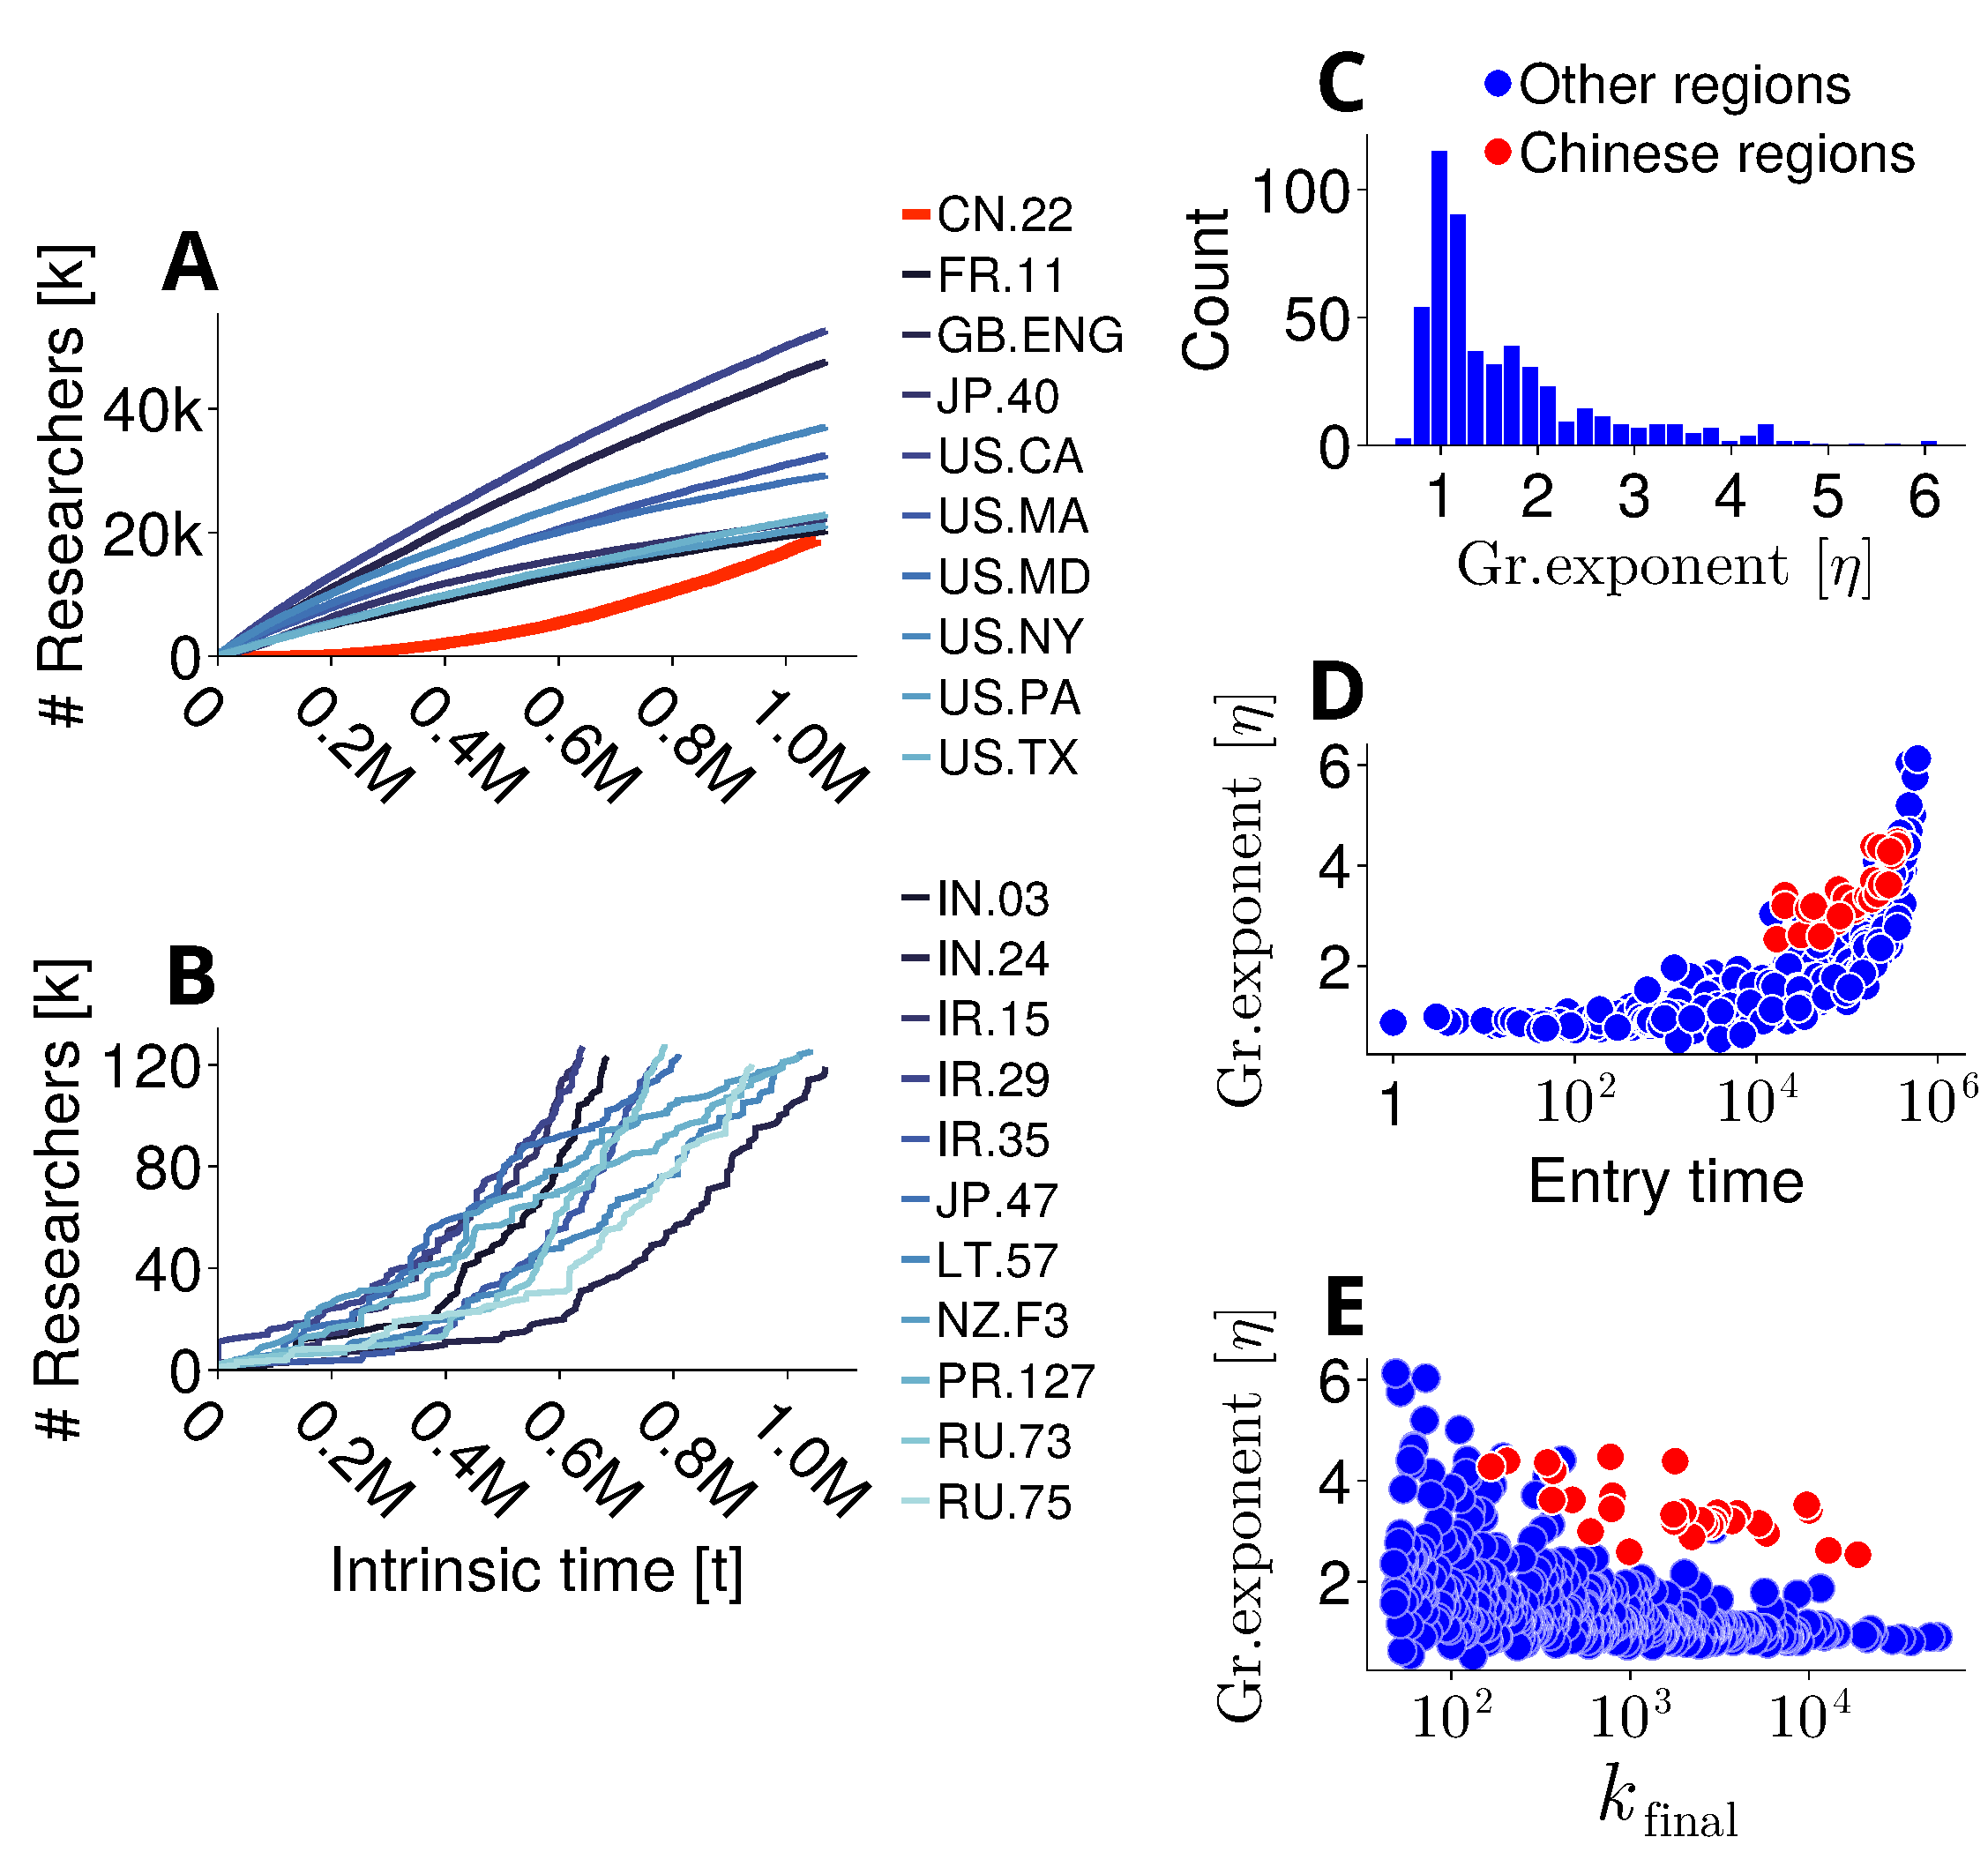
\includegraphics[width=0.8\linewidth]{figures_csf/fig3-cells.pdf}
    \caption{Panels A and B show the cumulative number of scientists coming into a region (lines) in intrinsic time in embryonic stem cell research; 
    with respect to Figs.~\ref{fig:sc-recap}~A and B, the axes are in linear scale to appreciate the different curvature of the growths at high intrinsic times;
    (A) shows the 10 most visited regions. Most regions grow sub-linearly. Chinese regions are shown with red thick lines and clearly increase super-linearly.
    In (B), we see 11 poorly visited regions ranked from 700 to 710 in terms of the number of scientists. Curves are (additively) shifted to the left so that their first point is placed at coordinates (1,1);
    (C) Histogram of growth exponents, $\eta$, for all regions;
    (D) Growth exponents, $\eta$, of all regions, $i$, as a function of their entry time, $t_i$ (intrinsic time). Note that Chinese regions (red) come in late (after timestep $10^5$) and have higher exponents than other regions (blue).
    (E) Growth exponents, $\eta$, as a function of the cumulative number of scientists in the year 2019, $k_{final}$. The high exponents of Chinese regions are visible (red).}
    \label{fig:cells-intrinsic_growth}
\end{figure}

\begin{figure}
    \centering
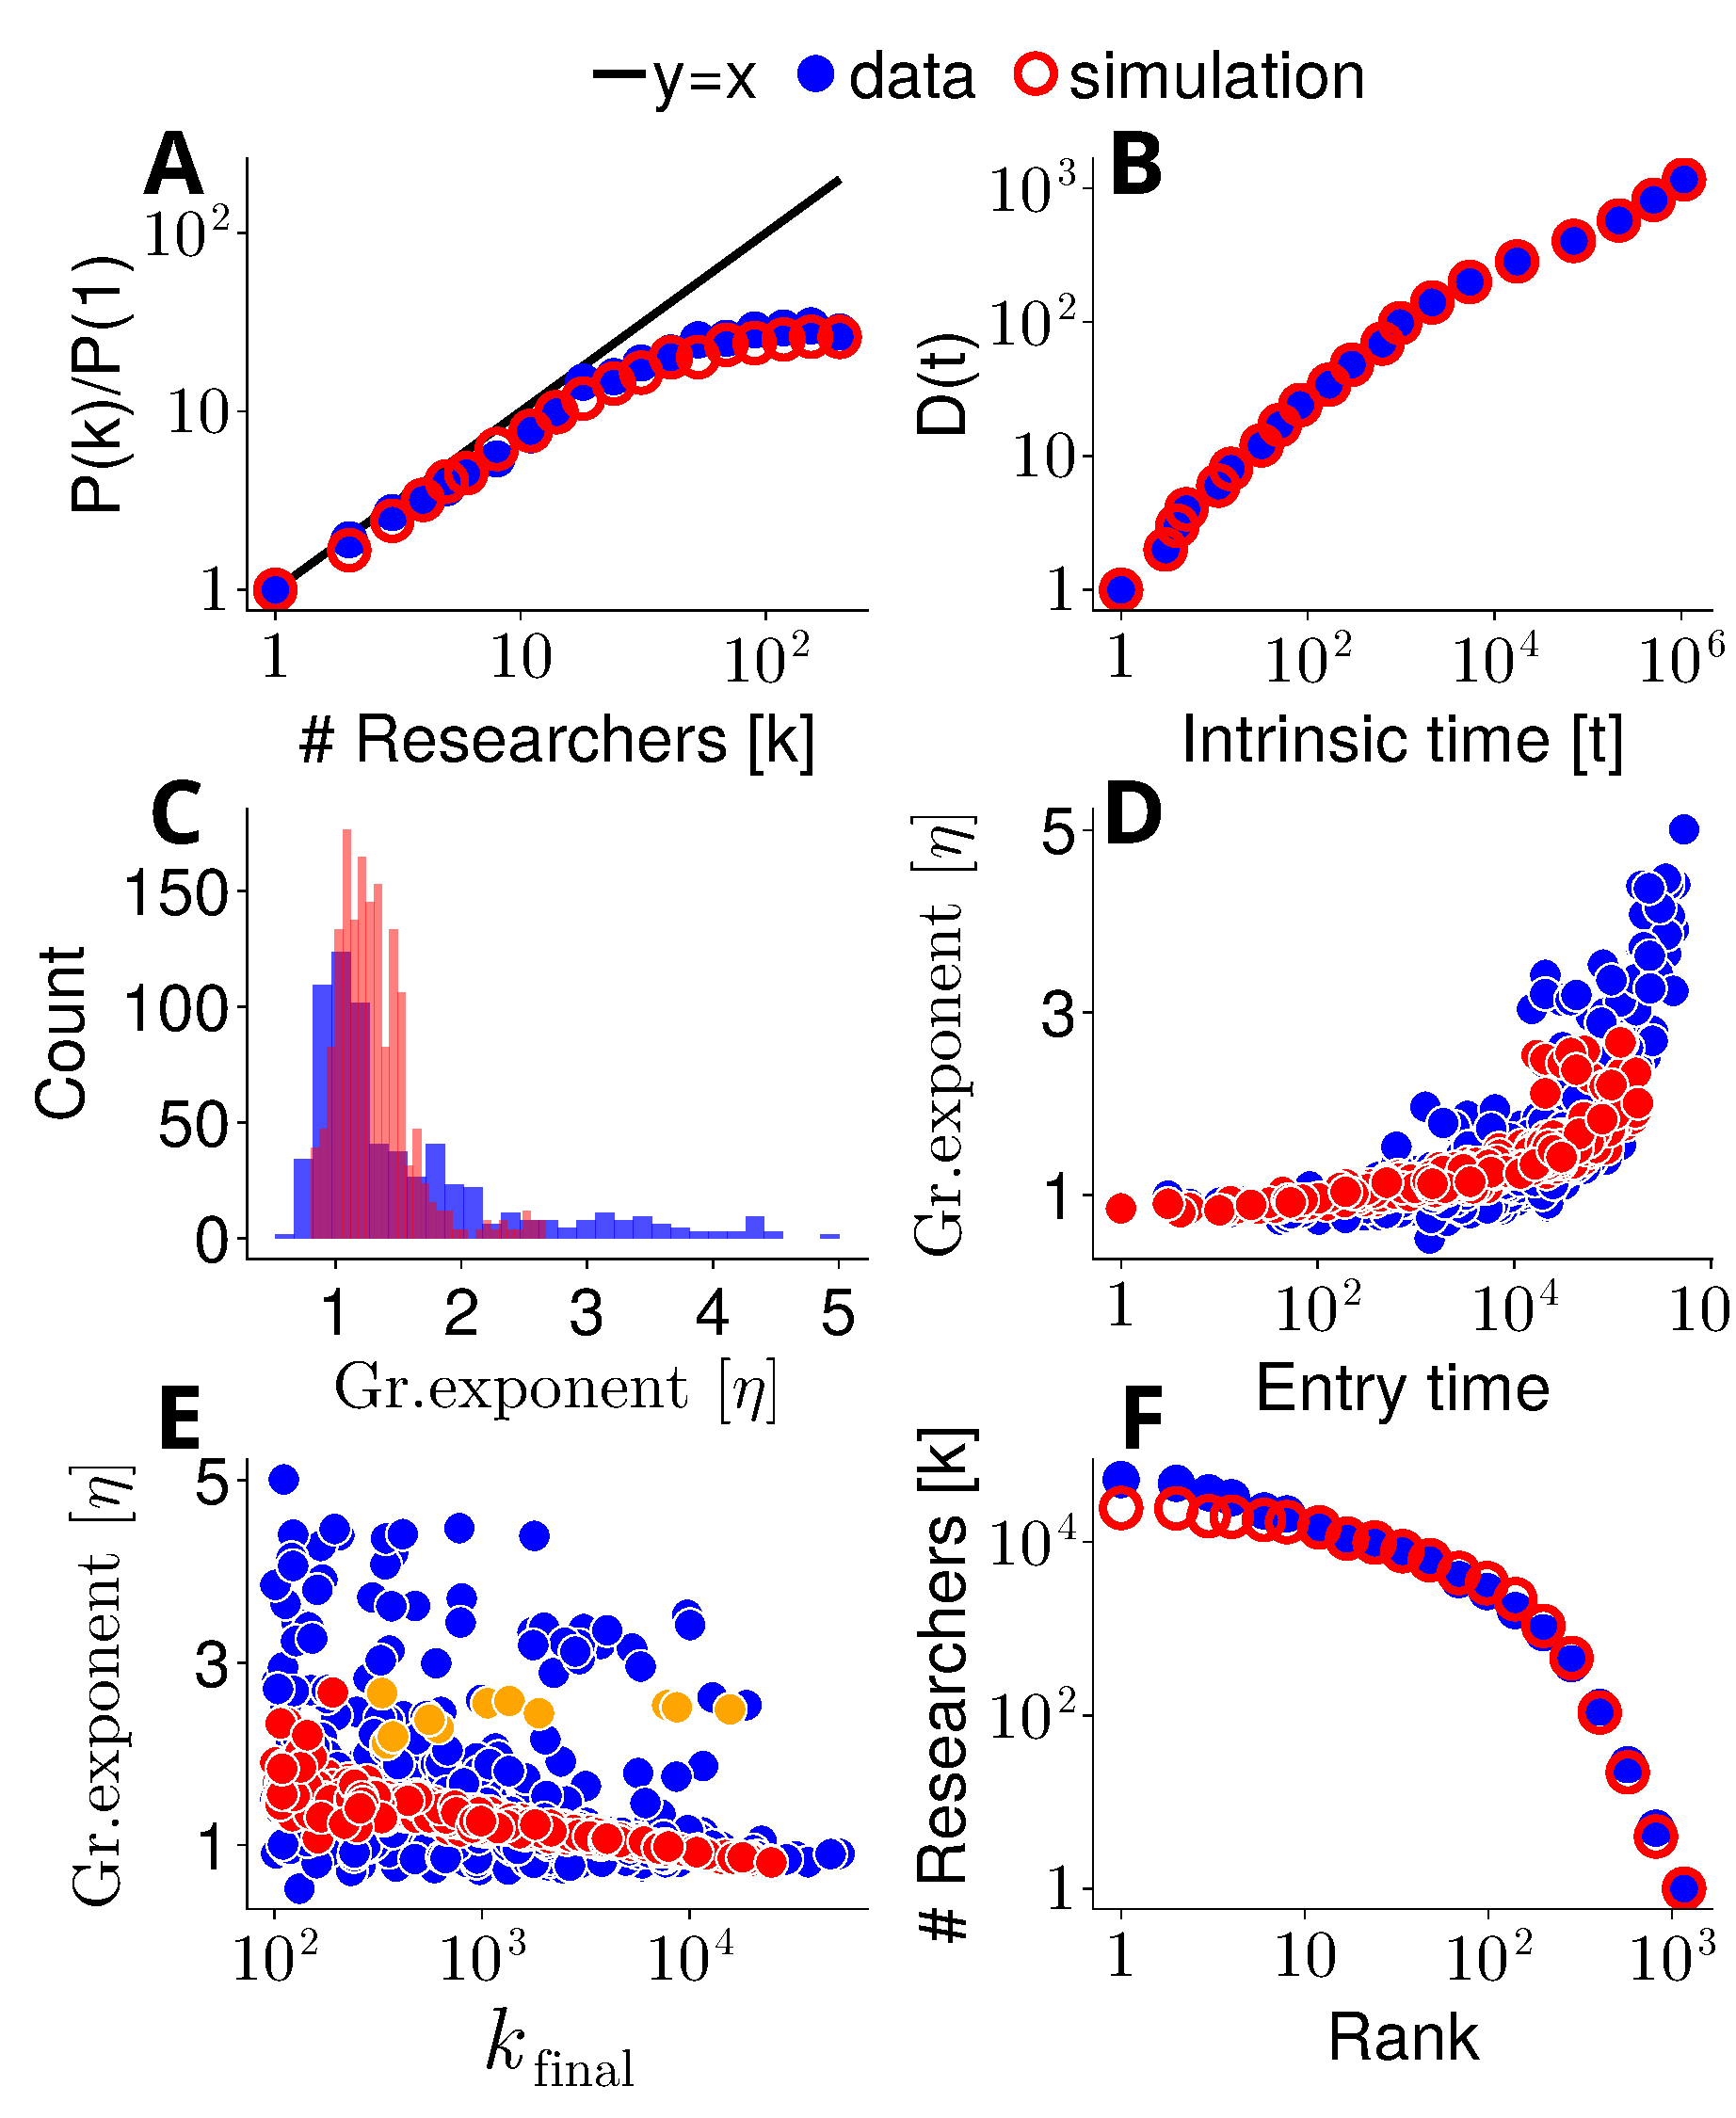
\includegraphics[width=0.8\linewidth]{figures_csf/fig4-cells.pdf}
    \caption{Comparison of model results (red) with experimental data  (blue) for the field of embryonic stem cells.
    (A) PA kernel; data and simulation practically coincide; the black line depicts a linear kernel.
    (B) Heaps's law; the two curves coincide by construction.
    (C) Histograms of the regional growth exponent, $\eta$.  
    The distributions of the empirical values have average $m=1.56$, standard deviation $s=0.86$ and skewness $b=1.73$, while the distribution of the simulated values has $m=1.31$, $s=0.31$ and $b=1.70$.
    (D) Exponents, $\eta$, reproduce the empirical increase as a function of entry time.
    (E) The decrease of $\eta$ as a function of the cumulative number $k_\mathrm{final}$ of scientists in the year 2019 is well captured by the model. Note the fact that Chinese regions (orange circles) are predicted with a higher than usual values.
    (F) Also the frequency-rank distributions of the regions appearing in the two streams practically coincide except for very small ranks.
    In panels C, D, and E only regions with $k_\mathrm{final}>100$ are taken into account.
    }
    \label{fig:cells-model}
\end{figure}


\subsection{Results for Internet research}
\label{app:internet}
Figures \ref{fig:internet-intrinsic_growth} and \ref{fig:internet-model} show the results for the field of Internet and share the same design of Figs. \ref{fig:sc-intrinsic_growth} and \ref{fig:sc-model}.

%%% INTERNET %%%

\begin{figure}[t] 
\centering
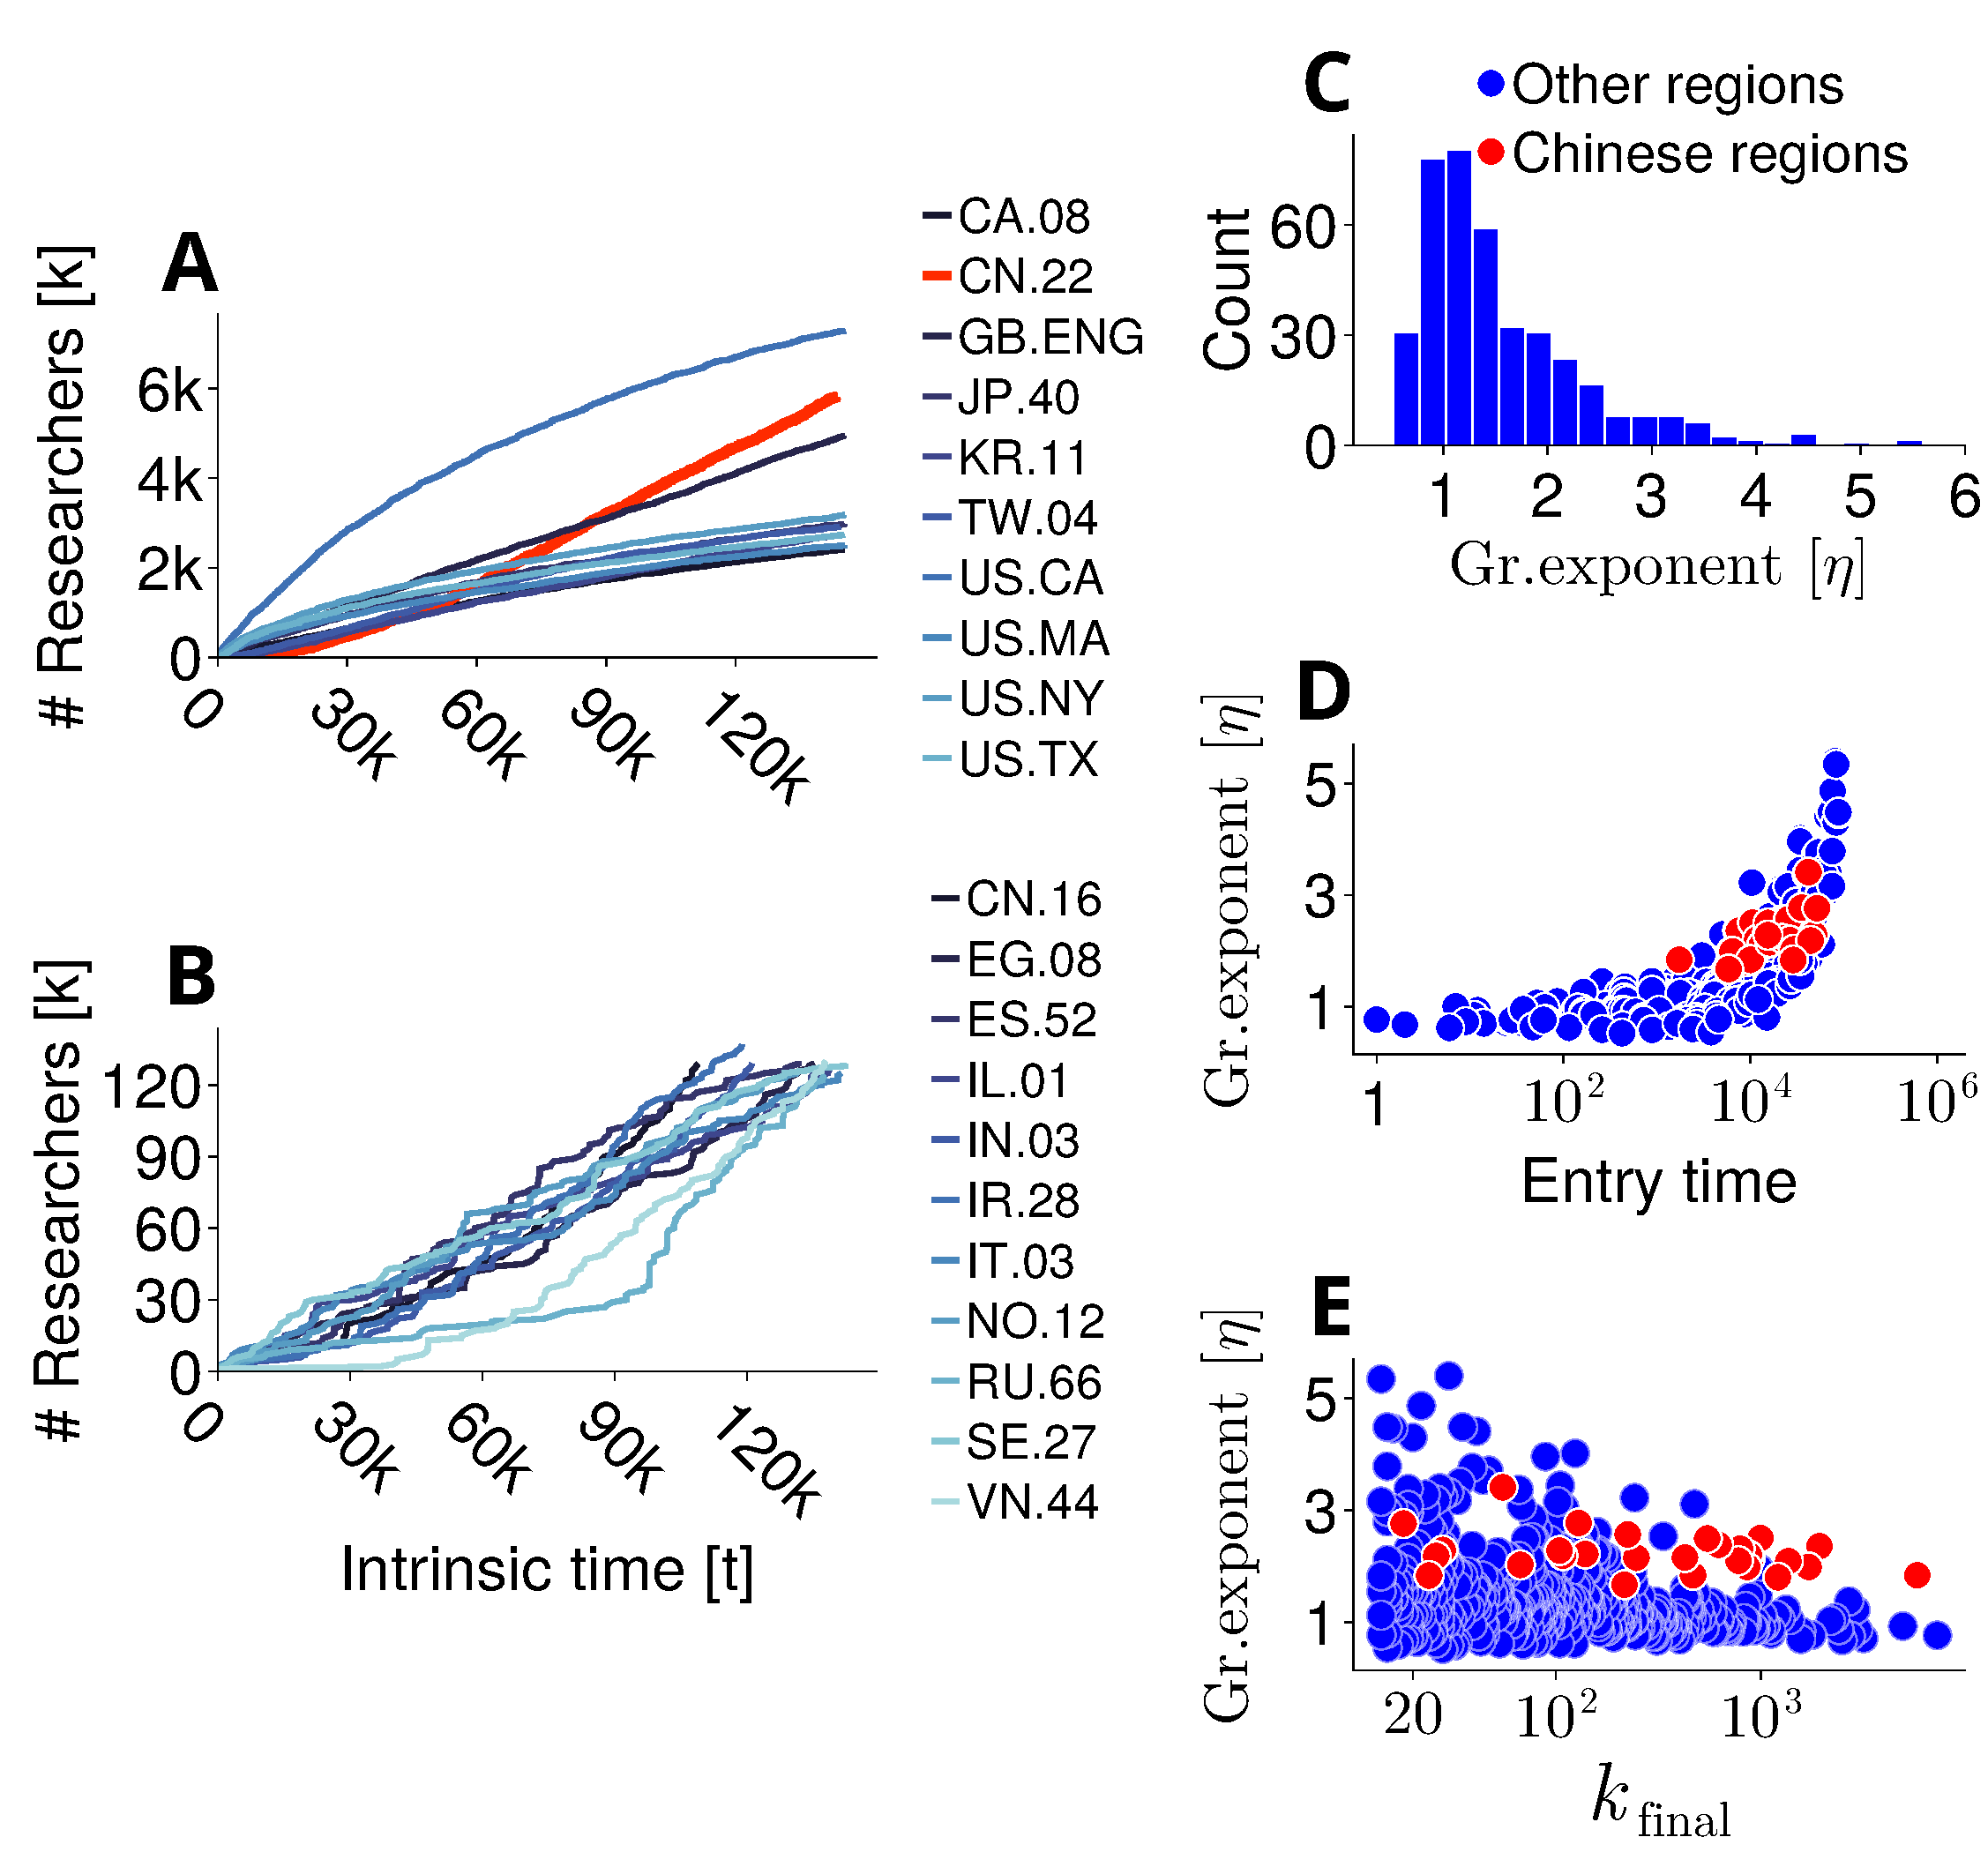
\includegraphics[width=0.8\linewidth]{figures_csf/fig3-internet.pdf}
    \caption{Panels A and B show the cumulative number of scientists coming into a region (lines) in intrinsic time in Internet research; 
        with respect to Figs.~\ref{fig:sc-recap}~A and B, the axes are in linear scale to appreciate the different curvature of the growths at higher intrinsic times;
    (A) shows the 10 most visited regions. Most regions grow sub-linearly. Chinese regions are shown with red thick lines and clearly increase super-linearly.
    In (B) we see 11 poorly visited regions ranked from 700 to 710 in terms of the number of scientists. Curves are (additively) shifted to the left so that their first point is placed at coordinates (1,1);
    (C) Histogram of growth exponents, $\eta$, for all regions;
    (D) Growth exponents, $\eta$, of all regions, $i$, as a function of their entry time, $t_i$ (intrinsic time). Note that Chinese regions (red) come in late (after timestep $10^5$) and have higher exponents than other regions (blue).
    (E) Growth exponents, $\eta$, as a function of the cumulative number of scientists in the year 2019, $k_{final}$. The high exponents of Chinese regions are visible (red).
    }
\label{fig:internet-intrinsic_growth}
\end{figure}

\begin{figure}[t]
    \centering
    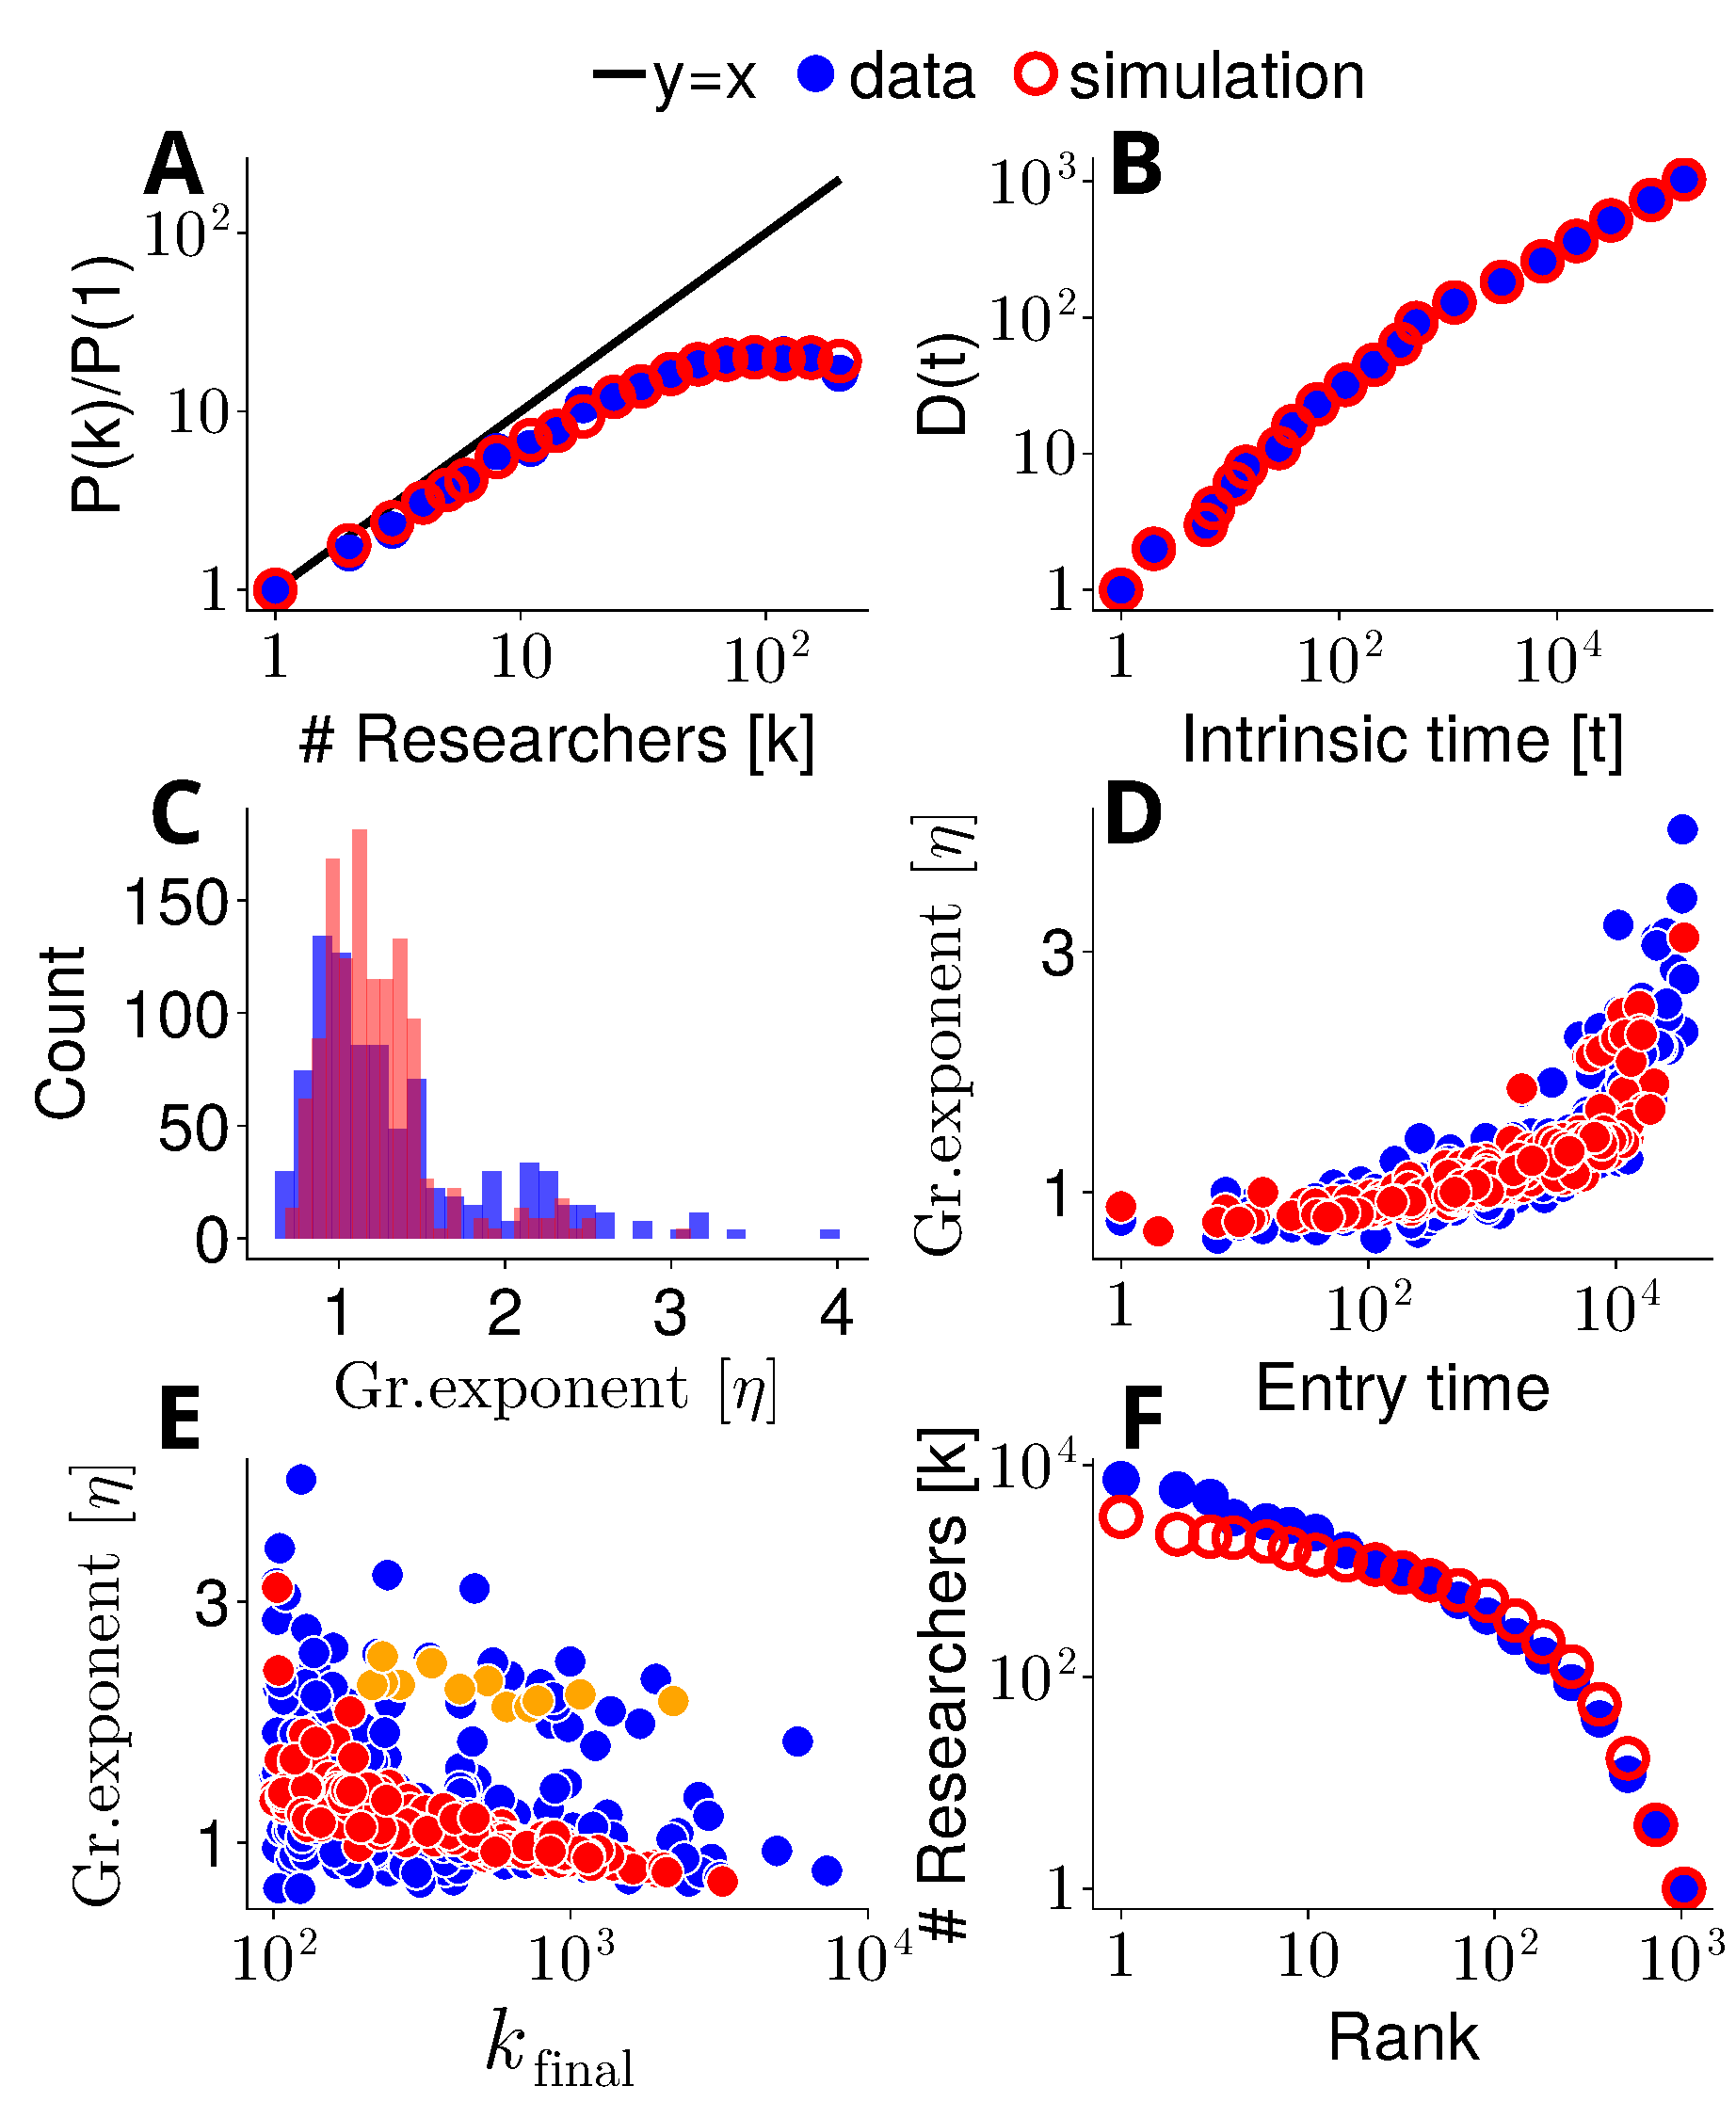
\includegraphics[width=0.8\linewidth]{figures_csf/fig4-internet.pdf}
    \caption{Comparison of model results (red) with experimental data  (blue) for the field of Internet.
    (A) PA kernel; data and simulation practically coincide; the black line depicts a linear kernel.
    (B) Heaps's law; the two curves coincide by construction.
    (C) Histograms of the regional growth exponent, $\eta$. 
    The distributions of the empirical values has average $m=1.36$, standard deviation $s=0.59$ and skewness $b=1.48$, while the distribution of the simulated values has $m=1.22$, $s=0.35$ and $b=1.93$.
    (D) Exponents, $\eta$, reproduce the empirical increase as a function of entry time.
    (E) The decrease of $\eta$ as a function of the cumulative number $k_\mathrm{final}$ of scientists in the year 2019 is well captured by the model. Note the fact that Chinese regions (orange circles) are predicted with higher than usual values.
    (F) Also, the frequency-rank distributions of the regions appearing in the two streams practically coincide except for very small ranks.
    In panels C, D, and E, only regions with $k_\mathrm{final}>100$ are taken into account.
    }
    \label{fig:internet-model}
\end{figure}

% ========================= CHAPTERS ======================================	
\chapter{Symbolic Capital: The Role of Social Media in Scientific Careers}
\todo{Enter your text here.}
% ========================= CHAPTERS ======================================	
\chapter{VII. Conclusion and Discussion}
\todo{Enter your text here.}
% Remove following line for the final thesis.
%%% intro.tex
%% Copyright (C) 2014-2020 by Thomas Auzinger <thomas@auzinger.name>
%
% This work may be distributed and/or modified under the
% conditions of the LaTeX Project Public License, either version 1.3
% of this license or (at your option) any later version.
% The latest version of this license is in
%   http://www.latex-project.org/lppl.txt
% and version 1.3 or later is part of all distributions of LaTeX
% version 2005/12/01 or later.
%
% This work has the LPPL maintenance status `maintained'.
%
% The Current Maintainer of this work is Thomas Auzinger.
%
% This work consists of the files vutinfth.dtx and vutinfth.ins
% and the derived file vutinfth.cls.
% This work also consists of the file intro.tex.


%\newacronym{ctan}{CTAN}{Comprehensive TeX Archive Network}
%\newacronym{faq}{FAQ}{Frequently Asked Questions}
%\newacronym{pdf}{PDF}{Portable Document Format}
%\newacronym{svn}{SVN}{Subversion}
%\newacronym{wysiwyg}{WYSIWYG}{What You See Is What You Get}

%\newglossaryentry{texteditor}
%{
%  name={editor},
%  description={A text editor is a type of program used for editing plain text files.}
%}

%\chapter{Introduction to \LaTeX}

%Since \LaTeX\ is widely used in academia and industry, there exists a plethora of freely accessible introductions to the language.
%Reading through the guide at \url{https://en.wikibooks.org/wiki/LaTeX} serves as a comprehensive overview for most of the functionality and is highly recommended before starting with a thesis in \LaTeX.

%\section{Installation}

%A full \LaTeX\ distribution\index{distribution} consists not only of the binaries that convert the source files to the typeset documents, but also of a wide range of packages and their documentation.
%Depending on the operating system, different implementations are available as shown in Table~\ref{tab:distrib}.
%\textbf{Due to the large amount of packages that are in everyday use and due to their high interdependence, it is paramount to keep the installed distribution\index{distribution} up to date.}
%Otherwise, obscure errors and tedious debugging ensue.

%\begin{table}
%  \centering
%  \begin{tabular}{cccc}
%    \toprule
%    Distribution & Unix         & Windows      & MacOS        \\
%    \midrule
%    TeX Live     & \textbf{yes} & yes          & (yes)        \\
%    MacTeX       & no           & no           & \textbf{yes} \\
%    MikTeX       & (yes)        & \textbf{yes} & yes          \\
%    \bottomrule
%  \end{tabular}
%  \caption{\TeX/\LaTeX\ distributions for different operating systems. Recomended choice in \textbf{bold}.}
%  \label{tab:distrib} % \label has to be placed AFTER \caption to produce correct cross-references.
%\end{table}

%\section{Editors}

%A multitude of \TeX\ \glspl{texteditor} are available differing in their editing models, their supported operating systems and their feature sets.
%A comprehensive overview of \glspl{texteditor} can be found at the Wikipedia page  \url{https://en.wikipedia.org/wiki/Comparison_of_TeX_editors}.
%TeXstudio (\url{http://texstudio.sourceforge.net/}) is recommended.
%Most editors support a synchronization of the generated document and the \LaTeX\ source by \verb|Ctrl| clicking either on the source document or the generated document.

%\section{Compilation}

%Modern editors usually provide the compilation programs to generate \gls{pdf} documents and for most \LaTeX\ source files, this is sufficient.
%More advanced \LaTeX\ functionality, such as glossaries and bibliographies, needs additional compilation steps, however.
%It is also possible that errors in the compilation process invalidate intermediate files and force subsequent compilation runs to fail.
%It is advisable to delete intermediate files (\verb|.aux|, \verb|.bbl|, etc.), if errors occur and persist.
%All files that are not generated by the user are automatically regenerated.
%To compile the current document, the steps as shown in Table~\ref{tab:compile} have to be taken.


%\begin{table}
%  \centering
%  \begin{tabular}{rl}
%    \toprule
%    & Description \\
%    \midrule
%    1 & Scan for refs, toc/lof/lot/loa items and cites \\
%    2 & Build the bibliography     \\
%    3 & Link refs and build the toc/lof/lot/loa \\
%    4 & Link the bibliography \\
%    5 & Build the glossary \\
%    6 & Build the acronyms \\
%   7 & Build the index \\
%    8 & Link the glossary, acronyms, and the index \\
%    9 & Link the bookmarks \\
%    \midrule
%    & Command \\
%    \midrule
%    1 & \verb|pdflatex.exe  example| \\
%    2 & \verb|bibtex.exe    example| \\
%    3 & \verb|pdflatex.exe  example| \\
%    4 & \verb|pdflatex.exe  example| \\
%    5 & \verb|makeindex.exe -t example.glg -s example.ist| \\
%      & \verb|              -o example.gls example.glo| \\
%    6 & \verb|makeindex.exe -t example.alg -s example.ist| \\
%      & \verb|              -o example.acr example.acn| \\
%    7 & \verb|makeindex.exe -t example.ilg -o example.ind example.idx| \\
%    8 & \verb|pdflatex.exe  example| \\
%    9 & \verb|pdflatex.exe  example| \\
%    \bottomrule
%  \end{tabular}
%  \caption{Compilation steps for this document. The following abbreviations were used: table of contents (toc), list of figures (lof), list of tables (lot), list of algorithms (loa).}
%  \label{tab:compile} % \label has to be placed AFTER \caption to produce correct cross-references.
%\end{table}


%\section{Basic Functionality}

%In this section, various examples are given of the fundamental building blocks used in a thesis.
%Many \LaTeX\ commands have a rich set of options that can be supplied as optional arguments.
%The documentation of each command should be consulted to get an impression of the full spectrum of its functionality.

%\subsection{Floats}

%Two main categories of page elements can be differentiated in the usual \LaTeX\ workflow: \textit{(i)} the main stream of text and \textit{(ii)} floating containers that are positioned at convenient positions throughout the document.
%In most cases, tables, plots, and images are put into such containers since they are usually positioned at the top or bottom of pages.
%These are realized by the two environments \verb|figure| and \verb|table|, which also provide functionality for cross-referencing (see Table~\ref{tab:intro} and Figure~\ref{fig:intro}) and the generation of corresponding entries in the list of figures and the list of tables.
%Note that these environments solely act as containers and can be assigned arbitrary content.

%\subsection{Tables}

%A table in \LaTeX\ is created by using a \verb|tabular| environment or any of its extensions, e.g., \verb|tabularx|.
%The commands \verb|\multirow| and \verb|\multicolumn| allow table elements to span multiple rows and columns.

%\begin{table}[h] % placement specifier
%  \centering
%  \begin{tabular}{lll}
%    \toprule
%    \multicolumn{2}{c}{Position} \\
%    \cmidrule{1-2} % partial horizontal rule
%    Group & Abbrev & Name \\
%    \midrule
%    Goalkeeper & GK & Paul Robinson \\
%    \midrule
%    \multirow{4}{*}{Defenders} & LB & Lucus Radebe \\
%                               & DC & Michael Duburry \\
 %                              & DC & Dominic Matteo \\
 %                              & RB & Didier Domi \\
 %   \midrule
 %   \multirow{3}{*}{Midfielders} & MC & David Batty \\
 %                                & MC & Eirik Bakke \\
  %                               & MC & Jody Morris \\
 %   \midrule
 %   Forward & FW & Jamie McMaster \\
 %   \midrule
 %   \multirow{2}{*}{Strikers} & ST & Alan Smith \\
%                              & ST & Mark Viduka \\
%    \bottomrule
%  \end{tabular}
 % \caption{Adapted example from the \LaTeX guide at \url{https://en.wikibooks.org/wiki/LaTeX/Tables}. This example uses rules specific to the \texttt{booktabs} package and employs the multi-row functionality of the \texttt{multirow} package.}
%  \label{tab:intro} % \label has to be placed AFTER \caption to produce correct cross-references.
%\end{table}

%\subsection{Images}

%An image is added to a document via the \verb|\includegraphics| command as shown in Figure~\ref{fig:intro}.
%The \verb|\subcaption| command can be used to reference subfigures, such as Figure~\ref{fig:intro:full width} and~\ref{fig:intro:half width}.

%\begin{figure}[h]
 % \centering
 % \begin{subfigure}[b]{0.45\columnwidth}
 %   \centering
%    
\includegraphics[width=\textwidth]{Logo-schwarz.pdf}
 %   \subcaption{The header logo at text width.}
 %   \label{fig:intro:full width}
%  \end{subfigure}
%  \begin{subfigure}[b]{0.45\columnwidth}
%    \centering
%    
\includegraphics[width=0.5\textwidth]{Logo-schwarz.pdf}
%    \subcaption{The header logo at half the text width.}
 %   \label{fig:intro:half width}
 % \end{subfigure}
 % \caption[Optional caption for the figure list (often used to abbreviate long captions)]{The header logo at different sizes.} % Remove the [...] argument if the original caption should be used in the figure list.
%  \label{fig:intro} % \label has to be placed AFTER \caption (or \subcaption) to produce correct cross-references.
%\end{figure}

%\subsection{Mathematical Expressions}

%One of the original motivation to create the \TeX\ system was the need for mathematical typesetting.
%To this day, \LaTeX\ is the preferred system to write math-heavy documents and a wide variety of functions aids the author in this task.
%A mathematical expression can be inserted inline as $\sum_{n=1}^{\infty} \frac{1}{n^2} = \frac{\pi^2}{6}$ outside of the text stream as \[ \sum_{n=1}^{\infty} \frac{1}{n^2} = \frac{\pi^2}{6} \] or as numbered equation with
%\begin{equation}
%\sum_{n=1}^{\infty} \frac{1}{n^2} = \frac{\pi^2}{6}.
%\end{equation}

%\subsection{Pseudo Code}

%The presentation of algorithms can be achieved with various packages; the most popular are \verb|algorithmic|, \verb|algorithm2e|, \verb|algorithmicx|, or \verb|algpseudocode|.
%An overview is given at \url{https://tex.stackexchange.com/questions/229355}.
%An example of the use of the \verb|alogrithm2e| package is given with Algorithm~\ref{alg:gauss-seidel}.

%\begin{algorithm}
%  \SetKw{BreakFor}{break for}
 % \KwIn{A scalar~$\epsilon$, a matrix $\mathbf{A} = (a_{ij})$, a vector $\vec{b}$, and an initial vector $\vec{x}^{(0)}$}
%  \KwOut{$\vec{x}^{(n)}$ with $\mathbf{A} \vec{x}^{(n)} \approx \vec{b}$}
%  \For{$k\leftarrow 1$ \KwTo maximum iterations}
%  {
%     \For{$i\leftarrow 1$ \KwTo $n$}
%     {
%        $x_i^{(k)} = \frac{1}{a_{ii}} \left(b_i-\sum_{j<i} a_{ij} x_j^{(k)} - \sum_{j>i} a_{ij} x_j^{(k-1)} \right)$\;
%     }
%     \If{$\lvert\vec{x}^{(k)}-\vec{x}^{(k-1)}\rvert < \epsilon$}
%     {\BreakFor\;}
%  }
%  \Return{$\vec{x}^{(k)}$\;}
%  \caption{Gauss-Seidel}
 % \label{alg:gauss-seidel} % \label has to be placed AFTER \caption to produce correct cross-references.
%\end{algorithm}

%\section{Bibliography}

%The referencing of prior work is a fundamental requirement of academic writing and well supported by \LaTeX.
%The \textsc{Bib}\TeX\ reference management software is the most commonly used system for this purpose.
%Using the \verb|\cite| command, it is possible to reference entries in a \verb|.bib| file out of the text stream, e.g., as~\cite{Turing1936}.
%The generation of the formatted bibliography needs a separate execution of \verb|bibtex.exe| (see Table~\ref{tab:compile}).

%\section{Table of Contents}

%The table of contents is automatically built by successive runs of the compilation, e.g., of \verb|pdflatex.exe|.
%The command \verb|\setsecnumdepth| allows the specification of the depth of the table of contents and additional entries can be added to the table of contents using \verb|\addcontentsline|.
%The starred versions of the sectioning commands, i.e., \verb|\chapter*|, \verb|\section*|, etc., remove the corresponding entry from the table of contents.

%\section{Acronyms / Glossary / Index}

%The list of acronyms, the glossary, and the index need to be built with a separate execution of \verb|makeindex| (see Table~\ref{tab:compile}).
%Acronyms have to be specified with \verb|\newacronym| while glossary entries use \verb|\newglossaryentry|.
%Both are then used in the document content with one of the variants of \verb|\gls|, such as \verb|\Gls|, \verb|\glspl|, or \verb|\Glspl|.
%Index items are simply generated by placing \verb|\index|\marg{entry} next to all the words that correspond to the index entry \meta{entry}.
%Note that many enhancements exist for these functionalities and the documentation of the \verb|makeindex| and the \verb|glossaries| packages should be consulted.

%\section{Tips}

%Since \TeX\ and its successors do not employ a \gls{wysiwyg} editing scheme, several guidelines improve the readability of the source content:
%\begin{itemize}
%\item Each sentence in the source text should start with a new line.
%      This helps not only the user navigation through the text, but also enables revision control systems (e.g. \gls{svn}, Git) to show the exact changes authored by different users.
%      Paragraphs are separated by one (or more) empty lines.
%\item Environments, which are defined by a matching pair of \verb|\begin{name}| and \verb|\end{name}|, can be indented by whitespace to show their hierarchical structure.
%\item In most cases, the explicit use of whitespace (e.g. by adding \verb|\hspace{4em}| or \verb|\vspace{1.5cm}|) violates typographic guidelines and rules.
%      Explicit formatting should only be employed as a last resort and, most likely, better ways to achieve the desired layout can be found by a quick web search.
%\item The use of bold or italic text is generally not supported by typographic considerations and the semantically meaningful \verb|\emph{|\texttt{$\dots$}\verb|}| should be used.
%\end{itemize}

%The predominant application of the \LaTeX\ system is the generation of \gls{pdf} files via the \textsc{Pdf}\LaTeX\ binaries.
%In the current version of \textsc{Pdf}\LaTeX, it is possible that absolute file paths and user account names are embedded in the final \gls{pdf} document.
%While this poses only a minor security issue for all documents, it is highly problematic for double blind reviews.
%The process shown in Table~\ref{tab:ps2pdf} can be employed to strip all private information from the final \gls{pdf} document.

%\begin{table}[h]
%  \centering
%  \begin{tabular}{rl}
%  \toprule
%  & Command \\
%  \midrule
%  1 & Rename the \gls{pdf} document \verb|final.pdf| to \verb|final.ps|. \\
%  2 & Execute the following command: \\
%    & \verb|ps2pdf -dPDFSETTINGS#/prepress ^| \\
%    & \verb| -dCompatibilityLevel#1.4 ^| \\
%    & \verb| -dAutoFilterColorImages#false ^| \\
%    & \verb| -dAutoFilterGrayImages#false ^| \\
%    & \verb| -dColorImageFilter#/FlateEncode ^| \\
%    & \verb| -dGrayImageFilter#/FlateEncode ^| \\
%    & \verb| -dMonoImageFilter#/FlateEncode ^| \\
%    & \verb| -dDownsampleColorImages#false ^| \\
%    & \verb| -dDownsampleGrayImages#false ^| \\
%    & \verb| final.ps final.pdf| \\
%  \bottomrule
%  \end{tabular}

%  On Unix-based systems, replace \verb|#| with \verb|=| and \verb|^| with \verb|\|.
%  \caption{Anonymization of \gls{pdf} documents.}
%  \label{tab:ps2pdf}
%\end{table}

%\section{Resources}

%\subsection{Useful Links}

%In the following, a listing of useful web resources is given.
%\begin{description}
%\item[\url{https://en.wikibooks.org/wiki/LaTeX}] An extensive wiki-based guide to \LaTeX.
%\item[\url{http://www.tex.ac.uk/faq}] A (huge) set of \gls{faq} about \TeX\ and \LaTeX.
%\item[\url{https://tex.stackexchange.com/}] The definitive user forum for non-trivial \LaTeX-related questions and answers.
%\end{description}

%\subsection[Comprehensive TeX Archive Network]{\gls{ctan}}

%The \gls{ctan} is the official repository for all \TeX\ related material.
%It can be accessed via \url{https://www.ctan.org/} and hosts (among other things) a huge variety of packages that provide extended functionality for \TeX\ and its successors.
%Note that most packages contain \gls{pdf} documentation that can be directly accessed via \gls{ctan}.

%In the following, a short, non-exhaustive list of relevant \gls{ctan}-hosted packages is given together with their relative path.
%\begin{description}[itemsep=0ex]
%\item[\href{https://www.ctan.org/pkg/algorithm2e}{algorithm2e}] Functionality for writing pseudo code.
%\item[\href{https://www.ctan.org/pkg/amsmath}{amsmath}] Enhanced functionality for typesetting mathematical expressions.
%\item[\href{https://www.ctan.org/pkg/amsfonts}{amssymb}] Provides a multitude of mathematical symbols.
%\item[\href{https://www.ctan.org/pkg/booktabs}{booktabs}] Improved typesetting of tables.
%\item[\href{https://www.ctan.org/pkg/enumitem}{enumitem}] Control over the layout of lists (\verb|itemize|, \verb|enumerate|, \verb|description|).
%\item[\href{https://www.ctan.org/pkg/fontenc}{fontenc}] Determines font encoding of the output.
%\item[\href{https://www.ctan.org/pkg/glossaries}{glossaries}] Create glossaries and list of acronyms.
%\item[\href{https://www.ctan.org/pkg/graphicx}{graphicx}] Insert images into the document.
%\item[\href{https://www.ctan.org/pkg/inputenc}{inputenc}] Determines encoding of the input.
%\item[\href{https://www.ctan.org/pkg/l2tabu}{l2tabu}] A description of bad practices when using \LaTeX.
%\item[\href{https://www.ctan.org/pkg/mathtools}{mathtools}] Further extension of mathematical typesetting.
%\item[\href{https://www.ctan.org/pkg/memoir}{memoir}] The document class on upon which the \verb|vutinfth| document class is based.
%\item[\href{https://www.ctan.org/pkg/multirow}{multirow}] Allows table elements to span several rows.
%\item[\href{https://www.ctan.org/pkg/pgfplots}{pgfplots}] Function plot drawings.
%\item[\href{https://www.ctan.org/pkg/pgf}{pgf/TikZ}] Creating graphics inside \LaTeX\ documents.
%\item[\href{https://www.ctan.org/pkg/subcaption}{subcaption}] Allows the use of subfigures and enables their referencing.
%\item[\href{https://www.ctan.org/tex-archive/info/symbols/comprehensive/}{symbols/comprehensive}] A listing of around 5000 symbols that can be used with \LaTeX.
%\item[\href{https://www.ctan.org/pkg/voss-mathmode}{voss-mathmode}] A comprehensive overview of typesetting mathematics in \LaTeX.
%\item[\href{https://www.ctan.org/pkg/xcolor}{xcolor}] Allows the definition and use of colors.
%\end{description} % A short introduction to LaTeX.

\backmatter

% Use an optional list of figures.
\listoffigures % Starred version, i.e., \listoffigures*, removes the toc entry.

% Use an optional list of tables.
\cleardoublepage % Start list of tables on the next empty right hand page.
\listoftables % Starred version, i.e., \listoftables*, removes the toc entry.

% Use an optional list of alogrithms.
%\listofalgorithms
%\addcontentsline{toc}{chapter}{List of Algorithms}

% Add an index.
\printindex

% Add a glossary.
\printglossaries

% Add a bibliography.
\bibliographystyle{alpha}
\bibliography{intro}

\end{document}